\documentclass[lang=cn,12pt]{elegantbook}
\title{信息论与编码理论: \LaTeX{}排版 }
\subtitle{笔记: 自用版}

\author{xiaowen}
%\institute{Elegant\LaTeX{} Program}
\date{\today}
%\version{4.3}
%\bioinfo{自定义}{信息}
\extrainfo{2021级信息与计算科学专业}%文档的附加信息

\setcounter{tocdepth}{3}
%控制 LaTeX 文档中目录(table of contents)的深度的命令。这个命令指定了在目录中包含多少级别的章节或标题。
%\setcounter{tocdepth}{0} 将只显示章节标题。
%\setcounter{tocdepth}{1} 将显示章节和子章节标题。
%\setcounter{tocdepth}{2} 将显示章节、子章节和子子章节标题。
%\setcounter{tocdepth}{3} 将显示章节、子章节、子子章节以及更深层级的标题,如果有的话。
\logo{logo-blue.png}
\cover{cover.jpg}%书籍的封面图

% 本文档命令
\usepackage{array}
\newcommand{\ccr}[1]{\makecell{{\color{#1}\rule{1cm}{1cm}}}}
%定义了一个新的命令 \ccr,它接受一个参数,用于创建带颜色的单元格,通常用于表格。
%\newcommand{\ccr}[1]: 这部分定义了一个新的命令 \ccr,它接受一个参数,这个参数在方括号 [1] 中指定。
%\makecell{}: 这是一个命令,通常由 makecell 宏包提供,用于更灵活地格式化表格单元格的内容。
%\color{#1}:这个部分使用给定的参数 #1 来设置单元格的文本颜色,#1 是您在使用 \ccr 命令时传递的颜色参数。
%\rule{1cm}{1cm}:这部分创建一个1厘米宽、1厘米高的有颜色的矩形框,作为单元格的内容。
\usepackage{graphicx}
\usepackage{subcaption}
\usepackage{tikz}
\usetikzlibrary{arrows.meta}
\numberwithin{equation}{section}

%\usepackage[dvipsnames]{xcolor}

\usepackage{tcolorbox}
\tcbuselibrary{breakable}
\usepackage{diagbox}

\usepackage{mdframed}
\mdfsetup{linewidth=1pt,linecolor=blue}
\mdfsetup{backgroundcolor=gray!10}
\mdfsetup{shadow=true}


% 修改标题页的橙色带
% \definecolor{customcolor}{RGB}{32,178,170}
% \colorlet{coverlinecolor}{customcolor}

\begin{document}

\maketitle
\frontmatter
%\frontmatter: 这个命令将文档切换到前言部分。在前言中,页码可能会使用罗马数字,并且章节编号可能会被隐藏。前言通常包括摘要、致谢等内容。
\tableofcontents
\mainmatter
%\mainmatter: 这个命令将文档切换到主体部分。在主体部分中,页码通常使用阿拉伯数字,并且章节和子章节的编号是可见的。主体部分包含文档的主要内容。
%\chapter{特殊的函数项级数——幂级数}
\chapter{引言}
在本章中,我们介绍信息论与编码理论的基本情况,使大家对信息理论和编码理论的全貌有一个大致的了解.

\begin{introduction}
 \item 信息论的早期酝酿
 \item Shannon信息论的建立与发展
 \item 信息论的近期发展
 \item 信息的度量问题
 \item 通信系统的基本要素与模型
 \item 通信系统的概率统计模型
\end{introduction}
\section{信息论的形成与发展}

\textbf{一、信息论的早期酝酿}

1.早期编码问题

在有线和无线电通信产生的同时,编码技术随之产生,早期的编码有Morse码和Bodo码.他们将文字通过点、划、空等信号给以表达,这些码虽然很原始,但它们实现了从文字到通讯信号的转变.中文通信等用的是电报码的方式,先将汉字转成数字,再用电码发射.

2.通信的有效性和可靠性

随着通信距离的加大,出现了信号强度衰减与噪声干扰的问题, 因此, 如何克服噪声千扰问题就成为通信技术中的一个迫切问题.为解决这些问题, 人们对通信中的各种因素进行分析, 发现在通信技术中,通信的数量与质量存在相互制约的关系.如果牺牲通信的数量, 则可以达到提高质量的目的, 但二者之间究竟有何定量关系,却无法说明.到了20世纪20 年代,奈奎斯特等人对上述问题进行了一系列讨论, 说明了信息传递的速率与带宽成正比,信息的度量与信号的概率分布、对数函数有关等等.

\textbf{二、Shannon信息论的建立与发展}

信息论的产生以1948年C.E.Shannon发表的 “通信的数学理论” 这一奠定性论文为起始,作为信息理论的奠基人,对其主要生平作一个简单的介绍.

Claude Edwoods Shannon(香农、仙农)  

C.E.Shannon(1916-2001) 数学家, 工程学家.信息论创始人,奠基人,电子计算机理论的重要奠基人之一.代表性著作:\\
(1)1938年(22岁),发表著名论文《继电器和开关电路的符号分析》文中首次使用了比特(bit)的概念.\\
(2) 1948年, 《通信的数字理论》第一次提出信息量的概念,并且应用数理统计的方法来研究通信系统, 从而创立了影响深远的信息论.\\
(3)1949年, 《噪声下的通信》经典的阐明了通信的基本问题, 提出了通信系统的模型, 给出了信息量的数字表达式, 解决了通道容量, 信源统计特性, 信源编码, 信道编码等有关精确地传递通信符号的基本技术问题.\\
(4)1956年, 《噪声信道的零差错容量》开拓了零差错容量的研究领域.\\
(5)1959年, 《在保真度准则下的离散信源编码定理》推动了信息率失真理论研究等.

Shannon提出完善信息理论离不开对编码问题的研究, 因此信息论与编码理论密不可分.

1.Shannon信息论的确立期(1948年-20世纪60年代)
此阶段主要是对Shannon理论进行研究与说明, 包括对通信系统的数学模型和基本问题的说明与讨论.

2.Shannon信息论的发展期(20世纪70-80年代)这一时期主要内容在 “率失真理论”与 “多用户信息论” 方面,后发展为数据压缩理论.

\textbf{三、信息论的近期发展}

信息论近期发展的主要特点是向多学科结合方向发展.

1. 信息论与密码学(通信编码问题的一种表现形式)

2. 算法信息论与分形数学 (信息论, 计算机科学, 分形理论的共同本质,决定如何互相等价转化).

3.信息论在统计与智能计算中的应用\\
(1) 智能计算中的信息统计问题.\\
(2)信息计算与组合投资决策关系密切.\\
(3)编码理论在与试验设计, 假设检验理论的结合中发挥了重要作用.

4.信息论在工程领域中的应用

主要是编码理论在工程领域有广泛应用.


\section{信息与编码理论的主要内容}

\textbf{一、信息的度量问题}

Shannon熵是Shannon信息论中信息的度量基础,它与概率分布有关,以不肯定性(不确定性)作为度量信息的基础,即信息量是描述消息中不确定性的概念.
例如:一个消息 “太阳从东边升起,西边落下”,这一消息中没有任何信息, 即含有的信息量为 0 .这是一确定的消息, 不含有任何的不肯定性(不确定性).


\textbf{二、通信系统的基本要素与模型}

1. 一个系统由以下基本要素与模型\\
(1)信源:产生信息的来源,信源产生的信息称为消息.\\
(2)信道:传递信息的通道,消息通过信道以信号的形式传播.\\
(3)编码:由消息产生信号的运算.\\
(4)译码:由信号还原为消息的运算称为译码.\\
(5)通信系统: 由信源、信道、编码和译码四个要素组成.\\
(6) 用户:通信系统的使用者,分为发送者和接收者.

2.通信系统的基本模型
\begin{figure}[ht]
    \centering
    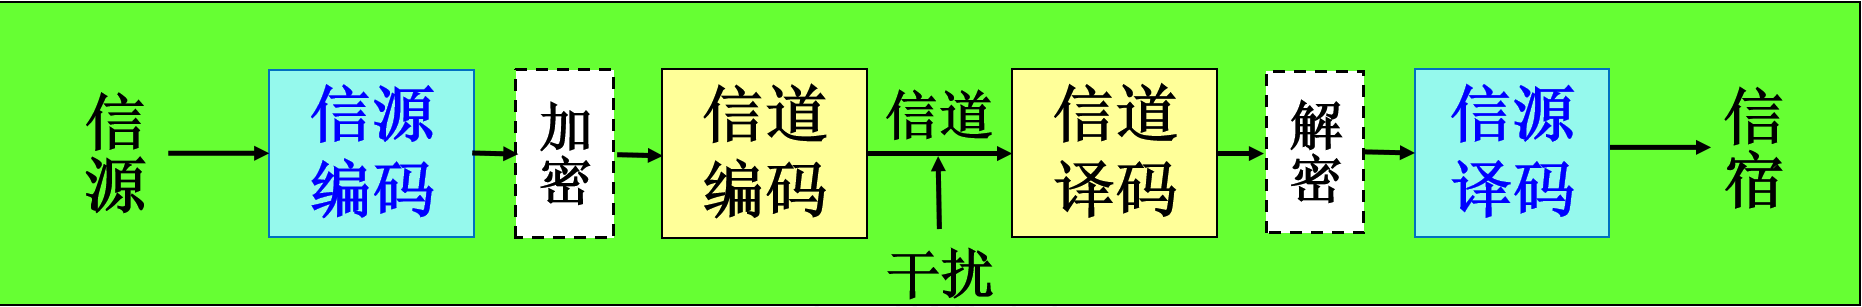
\includegraphics[width=0.5\linewidth]{image/0.png}
\end{figure}
由于干扰的存在, 信道的输出信号可能与输入信号不同, 从而使得还原消息与原始消息可能不同,这种现象称为通信误差,是通信系统中需要克服的现象.

克服通信误差 $ \left\{\begin{array}{l}\text { 硬件途径: 元器件改进, 降低噪声干扰 } \\ \text { 软件途径: 用编码方式克服 } \rightarrow \text { 纠错和检错码 }\end{array}\right. $


\textbf{三、通信系统的概率统计模型}

1. 信源的概率统计模型

\begin{definition}
    信源是消息的来源, 用 $ \mathscr{S}=[\mathscr{X}, p(x)] $ 来表示, 其中 $ \mathscr{X} $ 为信源字母表, 是消息中可能使用的全体符号, 它的元素 $ x \in \mathscr{X} $ 是信源字母表中的字母, $ p(x) $ 是字母 $ x $ 的使用概率.由概率分布的性质知, 对 $ \forall x \in \mathscr{X} $, 有 $ p(x) \geqslant 0 $,且 $ \sum\limits_{x \in \mathscr{X}} p(x)=1 $ .
\end{definition}


2. 信道的概率统计模型

信道由以下因素组成:输入信号字母集,输出信号字母集与转移概率分布, 分别记为\\ $ \{\mathscr{U}, \mathscr{V}, p(v \mid u), u \in \mathscr{U}, v \in \mathscr{V}\} $, 其中 $ \mathscr{U} $ 为全体能使用的输入信号字母集,简称为输入信号字母表, $ \mathscr{V} $ 是可能输出的信号字母集,简称为输出信号字母表.若 $ u \in \mathscr{U}, v \in \mathscr{V} $, 表示输入和输出信号字母, 而 $ p(v \mid u) $ 是输入、输出信号字母的转移概率, 即当输入信号为 $ u $, 输出信号为 $ v $ 的概率, 有 $ p(v \mid u) \geqslant 0, \sum\limits_{v \in \mathscr{V}} p(v \mid u)=1 $ .

\begin{definition}
    信道的概率统计模型为 $ \mathscr{C}=(\mathscr{U}, p(v \mid u), \mathscr{V}) $, 其中 $ \mathscr{U}, \mathscr{V} $ 分别是输入和输出信号字母表, $ p(v \mid u) $ 是输入和输出信号字母的转移概率.
\end{definition}



3. 编码与译码的函数表示
\begin{definition}
    由消息变为信道输入信号的运算称为编码,由信道输出信号变为还原消息的运算称为译码.记 $ \mathscr{Y} $ 为还原消息字母表.则 $ f: \mathscr{X} \rightarrow \mathscr{U}, g: \mathscr{V} \rightarrow \mathscr{Y} $ 分别是编码和译码运算, 在通信系统中,一般 $ \mathscr{U} $ 与 $ \mathscr{V} $ 相同,但也可以不同.
\end{definition}

4. 通信系统的数学模型
\begin{definition}
    称信源与信道的组合为通信系统, 记为
$$
\mathscr{E}=\{\mathscr{S}, \mathscr{C}\}=\{\mathscr{X}, p(x), \mathscr{U}, p(v \mid u), \mathscr{V}\}
$$
对于一个通信系统 $ \varepsilon $, 如果编码和译码函数 $ f, g $ 给定, 那么我们称这个通信系统是有编码的通信系统,记为
$$
\mathscr{E}(f, g)=\{\mathscr{S}, \mathscr{C},(f, g), \mathscr{Y}\}=\{\mathscr{X}, p(x), \mathscr{U}, p(v \mid u), \mathscr{V},(f, g), \mathscr{Y}\}
$$
\end{definition}


5. 由通信系统决定的随机变量

因为通信系统由一系列概率分布组成,因此我们可以用随机变量表示, 记:\\
$ \bar{\xi} $ 由信源 $ \mathscr{S}=\{\mathscr{X}, p(x)\} $ 决定的随机变量.\\
$ \xi $ 由信道输入信号决定的随机变量.\\
$ \eta $ 由信道输出信号决定的随机变量.\\
$ \bar{\eta} $ 由还原消息决定的随机变量.\\
$ \bar{\xi} $ 在 $ \mathscr{X} $ 上取值, 其概率分布为 $ p(x) $ .

\begin{theorem}
    如果有编码的通信系统 $ \mathscr{E}(f, g) $ 给定, 则这个通信系统的随机变量 $ (\bar{\xi}, \xi, \eta, \bar{\eta}) $ 的联合概率分布确定, 它们的联合概率分布 $ p(x, u, v, y)=p(x) f(u \mid x) p(v \mid u) g(y \mid v) $ ,其中 $ p(x), p(v \mid u) $ 分别由信源 $ S $ 和信道 $ C $ 给定.
$$
f(u \mid x)=\left\{\begin{array}{ll}
1, & u=f(x) \\
0, & u \neq f(x)
\end{array}\right.
$$
$$
g(y \mid v)=\left\{\begin{array}{ll}
1, & y=g(v) \\
0, & y \neq g(v)
\end{array}\right.
$$
这时, $ (\bar{\xi}, \xi, \eta, \bar{\eta}) $ 构成一个马尔可夫(Markov)链,因为当 $ \xi $ 固定时, $ \bar{\xi} $ 与相互独立,而当 $ \eta $ 固定时, $ (\bar{\xi}, \xi) $ 与 $ \bar{\eta} $ 相互独立.
\end{theorem}

有关概率记号: $ p(x, u, v, y)=P_{r}\{(\bar{\xi}, \xi, \eta, \bar{\eta})=(x, u, v, y)\} $
$$
\begin{array}{l}
p(x)=\operatorname{Pr}\{\bar{\xi}=x\} \\
p(v \mid u)=\operatorname{P} r\{\eta=v \mid \xi=u\}
\end{array}
$$
其中, $ P_{r}(A) $ 表示事件 $ A $ 发生的概率, $ P_{r}(A \mid B) $ 表示事件 $ A $ 关于事件 $ B $ 的条件概率.
$$
P(A)=P_{r}(A) \quad P(A \mid B)=P_{r}(A \mid B)
$$

\begin{definition}
    如果随机变量 $ (\bar{\xi}, \xi, \eta, \bar{\eta}) $ 的概率分布为 $ p(x, u, v, y)=p(x) f(u \mid x) p(v \mid u) g(y \mid \underline{v}) $, 则称 $ (\bar{\xi}, \xi, \eta, \bar{\eta}) $ 是由通信系统 $ \mathscr{E}(f, g) $ 决定的随机变量, 如果 $ (\bar{\xi}, \xi, \eta, \bar{\eta}) $ 构成一个马尔可夫链, 那么记之为:
$$
\bar{\xi} \longrightarrow \xi \longrightarrow \eta \longrightarrow \bar{\eta}
$$
\end{definition}

\section{本书基本内容与参考文献}

\textbf{一、基本内容}
\begin{enumerate}
    \item 信息论部分:
    \begin{enumerate}
        \item 信息的度量和性质
        \item 信源和信道的编码问题及编码定理
    \end{enumerate}
    \item 编码理论部分
\begin{enumerate}
    \item 代数码的概念和性质
    \item 几种典型的代数码 (Hamming码, 循环码)
\end{enumerate}
\end{enumerate}
\textbf{二、前续知识:}
\begin{itemize}
    \item 概率论
    \item 抽象代数(近世代数)
\end{itemize}
\textbf{三、参考文献}

\begin{itemize}
    \item Coding and Information Theory.Steven Roman.Springer.
    \item 万哲先. 代数和编码 (第三版). 北京.高等教育出版社.
    \item 叶中行. 信息论基础.高等教育出版社.
    \item 曹雪虹, 张宗橙. 信息论与编码, 北京邮电大学出版社.
\end{itemize}



\chapter{信息量}
\section{熵}
设信源 $ \mathscr{S}=\{\mathscr{X}, p(x)\} $ 为离散信息, $ \bar{\xi} $ 为一随机变量, 取自 $ \mathscr{S} $ . 如: 随机事件掷骰子. 信源集 $ \mathscr{X}=\{1,2,3,4,5,6\} $ 的概率分布为 $ \left(\begin{array}{cccccc}1 & 2 & 3 & 4 & 5 & 6 \\ \frac{1}{6} & \frac{1}{6} & \frac{1}{6} & \frac{1}{6} & \frac{1}{6} & \frac{1}{6}\end{array}\right) $ ,$ \bar{\xi} $ 取某一可能, 如 $ \bar{\xi}=4 $, 则 $ \bar{\xi} $ 带有多少信息量与 4 的概率有关, 即与不确定性有关.此时, $ \bar{\xi}=4 $ 提供了多少信息.


一般地 $ \mathscr{X}=\left\{x_{1}, x_{2}, \cdots, x_{a}\right\} $, 其中 $ a $ 为某个正整数, 对 $ \forall x_{i} \in \mathscr{X} $, $ \bar{\xi} $ 取值为 $ x_{i} $ 的概率为
$$
p_{i}=p\left(\xi_{i}\right)=P_{r}\left(\xi=x_{i}\right), i=1,2, \cdots, a .
$$
$ \bar{\xi} $ 和它的概率分布表示为 $ \left(\begin{array}{llll}x_{1} & x_{2} & \cdots & x_{a} \\ p_{1} & p_{2} & \cdots & p_{a}\end{array}\right) $, 
则有 $ p_{i} \geqslant 0, i=1,2, \cdots, a, \sum\limits_{i=1}^{a} p_{i}=1 $ .

$ \bar{\xi} $ 取某一信号 $ x_{i}, \bar{\xi}=x_{i} $, 带有多少信息量, 与 $ x_{i} $ 的概率有关, 即与不确定性有关.

\subsection{自信息量}
\begin{definition}
    一个随机事件发生某一结果后所带来的信息量称为自信息量. 定义为其发生概率的对数的负值.即若随机事件$x_i$ 发生的概率为 $p(x_i)$, 那么它的自信息量为 $$I(x_i)=-\log p(x_i)$$
\end{definition}

由于 $ x_{i} $ 是随机出现的, 它是 $ \mathscr{X} $ 的一个样值, 所以是一个随机量.而 $ I\left(x_{i}\right) $ 是 $ x_{i} $ 的函数, 它必须也是一个随机量.

自信息量的单位与所用的对数底有关.在信息论中常用的对数底是 2 ,信息量的单位为比特 (bit); 若取自然对数, 则信息量的单位为奈特 (nat); 若以 10 为对数底, 则信息量的单位为笛特 (det).这三个信息量单位之间的转换关系如下:
$$
1 \text { nat }=\log _{2} \mathrm{e} \approx 1.433 \mathrm{bit}, \quad 1 \mathrm{det}=\log _{2} 10 \approx 3.322 \mathrm{bit}
$$
\begin{note}
    信息量是纯数,信息量单位只是为了标示不同底数的对数值,并无量纲的含义.
\end{note}


    自信息量的特点是,当事件的概率越小,其自信息量越大,表示提供的信息越多;而当事件的概率越大,其自信息量越小,表示提供的信息越少.当事件的概率越小,其自信息量越大的原因可以通过信息的意外性来解释.假设一个事件的概率非常小,意味着这个事件发生的可能性非常低,它是一种罕见或异常的情况.当这个罕见事件发生时,它提供了大量的信息,因为它与我们的预期或常见情况相悖,具有较高的意外性.


这里要引入随机事件的不确定度概念.根据日常知识, 各个出现概率不同的随机事件所包含的不确定度是有差别的.一个出现概率接近于 1 的随机事件, 发生的可能性很大, 所以它包含的不确定度就很小.反之, 一个出现概率很小的随机事件, 很难猜测在某个时刻它能否发生, 所以它包含的不确定度就很大.若是确定性事件, 出现概率为 1 , 则它包含的不确定度为 0 .

\begin{remark}
   \textbf{ 随机事件的不确定度在数量上等于它的自信息量, 两者的单位相同, 但含义却不相同.}具有某种概率分布的随机事件不管发生与否, 都存在不确定度, 不确定度表征了该事件的特性,而自信息量是在该事件发生后给予观察者的信息量.
\end{remark}
 
\subsection{不确定性(自信息量)的性质}

上述自信息函数 $ I\left(x_{i}\right) $ 应满足以下性质:

(1) $ p\left(x_{i}\right) $ 越大, $ I\left(x_{i}\right) $ 越小, 即 $ I(x) $ 是关于 $ P(x) $ 单调递减的;

(2) $ x, y $ 是相互独立的两个信号, 即联合分布 $ p(x, y)=p(x) p(y) $ 时,$ I(x, y)=I(x)+I(y) $ .

于是, 可推出自信息函数 $ I(x) $ 应满足以下公理:
\begin{axiom}
( i ) $ I(x) \geqslant 0 $;

(ii) 当$ p(x)=1$时, $I(x)=0 $;

(iii ) 当$ p(x)=0$时,$ I(x)=\infty $;

(iv)若 $ p(x)>p(y) $ ,则 $ I(x)<I(y) $;

 (v)  若 $ p(x, y)=p(x) p(y) $, 则 $ I(x, y)=I(x)+I(y) $ .
\end{axiom}
\begin{note}
    (1) 信息量非负说明随机事件发生后总能提供一些信息量,最差情况是零,即什么信息也没提供,但不会因事件发生使得不确定性更大.$P_i$表示随机事件发生的概率,在闭区间$[0,1]$上取值,根据对数的性质也可知$I(x)\geqslant 0$.

    (2)当$ p(x)=1$时, 说明该事件是必然事件. 必然事件不含有任何不确定性,所以不含任何信息量.

    (3)当一个事件的概率接近于1时,它的信息量趋近于0,表示这个事件是高度可预测的,提供的信息量很少. 相反,当一个事件的概率接近于0时,它的信息量趋近于正无穷大,表示这个事件是高度意外的,提供的信息量很大.

    (4)概率越大的事件,不确定性越小,发生后提供的信息量就越小.即$I(x)$是$p_i$的单调递减函数.

    (5)首先,根据独立事件的定义,事件$x$和$y$的联合概率等于它们的边缘概率的乘积,即$p(x, y) = p(x) \cdot p(y)$.然后,根据自信息的定义,$I(x) = -\log p(x)$和$I(y) = -\log p(y)$. 将上述两个式子代入$I(x, y)$的定义中,有:$I(x, y) = -\log p(x, y) = -\log (p(x) \cdot p(y))$. 根据对数运算的性质,上式可以改写为:
$I(x, y) = -\log p(x) - \log p(y) = I(x) + I(y)$. 因此,当事件$x$和$y$是独立事件且满足$p(x, y) = p(x) \cdot p(y)$时,可以得出$I(x, y) = I(x) + I(y)$的结论. 这意味着两个独立事件的联合自信息等于它们各自的自信息之和.
\end{note}


于是, 要对信息量进行度量 (定量表示) , 需要寻求一个满足上述条件的自信息函数.

\subsection{自信息函数的推导}
\begin{lemma}
若实函数 $ f(x)(1 \leqslant x \leqslant \infty) $ 满足以下条件:\\
( i ) $ f(x) \geqslant 0 $;\\
(ii) $ f(x) $ 是严格单调增加的, 即 $ x<y \Rightarrow f(x)<f(y) $ :\\
(iii) $ f(x \cdot y)=f(x)+f(y) $ :

则有 $ f(x)=c \log x $ ,其中 $ c $ 为常数.


\end{lemma}

\begin{proof}
    反复使用  (iii), 对任意正整数 $ k $, 我们有
$$
f\left(x^{k}\right)=f\left(x \cdot x^{k-1}\right)=f(x)+f\left(x^{k-1}\right)=\cdots=k f(x)
$$
从而 $ f(1)=0 $. 进而由于 (i) 和 (ii) , 对于任意 $ x>1, f(x)>0 $, 对于任意大于 1 的 $ x, y $与任意正整数 $ k $, 总可以找到非负整数 $ n $, 使
$$
y^{n} \leqslant x^{k}<y^{n+1}
$$
(事实上, 由 $ y>1 $, 则区间 $ (1,+\infty) $ 可由 $ y $ 分为 $ (1, y],\left(y, y^{2}\right],\left[y^{2}, y^{3}\right], \cdots, x $ 取定, $ x^{k} $ 是固定的正函数,必落在某个区间内.)


取对数并除以 $ k \log_a y $ 得
\begin{equation}
\frac{n}{k} \leqslant \frac{\log_a x}{\log_a y}<\frac{n+1}{k}\label{eq1}
\end{equation}
另一方面, 由$f\left(x^{k}\right)=k f(x)$结合条件 (ii)可得
$$
n f(y) \leqslant k f(x)<(n+1) f(x)
$$
两边同时除以 $ k f(y) $ 得:
$$
\frac{n}{k} \leqslant \frac{f(x)}{f(y)}<\frac{n+1}{k}
$$
两边同时乘以$-1$得:
\begin{equation}
-\frac{n+1}{k} \leqslant-\frac{f(x)}{f(y)} \leqslant-\frac{n}{k}\label{eq2}
\end{equation}
于是联立\eqref{eq1}和\eqref{eq2}得:
$$
-\frac{1}{k} \leqslant \frac{\log _{c} x}{\log _{c} y}-\frac{f(x)}{f(y)} \leqslant \frac{1}{k}
$$
我们有
$$
\left|\frac{f(x)}{f(y)}-\frac{\log_a x}{\log_a y}\right| \leqslant \frac{1}{k}
$$
当 $ k \rightarrow \infty $ 时,
$$
\frac{f(x)}{f(y)}=\frac{\log_a x}{\log_a y}
$$
因此,
$$
\frac{f(x)}{\log_a x}=\frac{f(y)}{\log_a y}=c
$$
或
$$
f(x)=c \log_a x
$$
\end{proof}
\begin{remark}
  对于自信息函数 $ I(x)=I(p(x)) $, 令 $ t=\frac{1}{p(x)} $,则 $ I(t)=I\left(\frac{1}{p(x)}\right), I(x) $ 关于 $ p(x) $ 递减,又 $ I(t(x), t(y))=I(t(x))+I(t(y)) $ 成立,由引理知: $ I(t)=c \log _{a} t $, 从而 $ I(x)=c \log _{a} \frac{1}{p(x)} $ .
\end{remark}

\begin{theorem}
    若自信息 $ I(x) $ 满足5条公理, 则 $ I(x)=c \log _{a} \frac{1}{p(x)} $, 其中 $ c $ 为常数, 此时称 $ I(x) $ 为自信息函.
\end{theorem}

设 $ x \in \mathscr{X}, x $ 具有概率分布 $ p(x) $, 则 $ x $ 的自信息定义为
$$
I(x)=\log _{a} \frac{1}{p(x)}
$$
\subsection{香农熵的定义(Shannon 熵)}
信源 $ \mathscr{S}=\{\mathscr{X}, p(x)\},  \xi $ 是随机变量(考虑随机信号的信息量).

前面介绍 $ x \in \mathscr{X} $ 的自信息是在 $ X $ 确定的情况下,现在 $ \xi $ 是随机变量,发送哪一个信号是不确定的,因此需考虑在信号随机选取时携带的信息量如何刻画,即对整个信源,每个信号的平均信息量为多少?

\begin{definition}
   如果一个离散随机变量 $ \xi $ 的概率分布为 $\bar{p}=\left(p_{1}, p_{2}, \cdots, p_{a}\right)$, 则它的熵 $H(\xi)$或  $H(\bar{p})$定义为 
$$
\begin{aligned}
H(\xi)&=H\left(p_{1}, p_{2}, \cdots, p_{a}\right)=-\sum_{i=1}^{a} p_{i} \log _{c} p_{i} \\
&=\sum_{i=1}^{a} p_{i} \log _{c} \frac{1}{p_{i}}=E\left(\log _{c} \frac{1}{p}\right)
\end{aligned}
$$ 
\end{definition}
\begin{remark}

(1) $ H(\xi) $ 是 $ \log _{c} \frac{1}{p(\xi)} $ 的期望值

(2) 底数 $ c=2 $ 时, $ H(\xi) $ 的单位规定为比特;

底数 $ c=e $ 时, $ H(\xi) $ 的单位规定为奈特;

底数 $ c=3 $ 时, $ H(\xi) $ 的单位规定为铁特;

各个单位之间可根据对数的换底公式进行换算;如: $ \log _{2} \frac{1}{p_{i}}=\frac{\log _{e} \frac{1}{p_{i}}}{\log _{e} 2} $

(3) 除特别说明外, 取 $ c=2 $.
\end{remark}

\subsection{熵的简单性质与例子}

 $ H\left(p_{1}, p_{2}, \cdots, p_{a}\right) $ 为上述定义的Shannon熵,则其满足以下性质:
 
(1) 对称性: $ H\left(p_{1}, p_{2}, \cdots, p_{a}\right)=H\left(p_{\sigma(1)}, p_{\sigma(2)}, \cdots, p_{\sigma(a)}\right) $其中 $ \sigma $ 为有限集 $ \{1,2, \cdots, a\} $ 的一个置换.

(2)非负性:对任意的概率分布 $ \bar{p}=\left\{p_{1}, p_{2}, \cdots, p_{a}\right\} $ ,有 $ H\left(p_{1}, p_{2}, \cdots, p_{a}\right) \geqslant 0 $, 且等号成立当且仅当 $ \bar{p} $ 是一个确定性分布 (其中一个取 1 , 其它的取 0 ).

证明:(1) 显然当概率的顺序发生置换后,只是求和顺序不同,并不影响求和结果. (平均值, 数学期望).

(2) $ \Leftarrow $ : 显然
$$
\Rightarrow: H\left(p_{1}, p_{2}, \cdots, p_{a}\right)=0 \text {, 由 } H\left(p_{1}, p_{2}, \cdots, p_{a}\right) \text { 的 }
$$
定义可知, $ \forall i, p_{i} \log _{c} p_{i}=0 $, 或者 $ p_{i}=0 $, 或者 $ \log _{c} p_{i}=0 $, 由于 $ \sum\limits_{i=1}^{a} p_{i}=1, p_{i} \geq 0 $, 存在 $ i $ 使得 $ p_{i}=1 $, 而其它 $ p_{j}=0 $, 因此 $ \bar{p} $ 必为确定型分布.


\begin{example}
    以等概率 $ p_{i}=\frac{1}{3} $ 从集合 $ \mathscr{X}=\left\{x_{1}, x_{2}, x_{3}\right\} $ 中抽样,以 $ p_{1}=p_{2}= $ $ \frac{1}{4}, p_{3}=\frac{1}{2} $ 从集合 $ \mathscr{X}=\left\{x_{1}, x_{2}, x_{3}\right\} $ 中抽样, 以上两个随机事件那个信息量大? (不确性大, 信息量越大)

    解: 设两个随机事件的随机变量分别为 $ \xi_{1}, \xi_{2} $, 则有
$$
\begin{aligned}
H\left(\xi_{1}\right) & =\sum_{i=1}^{3} p_{i} \log _{2} \frac{1}{p_{i}} \\
& =\left(\frac{1}{3} \log _{2} 3+\frac{1}{3} \log _{2} 3+\frac{1}{3} \log _{2} 3\right) \\
& =\log _{2} 3 \approx 1.585 \\
H\left(\xi_{2}\right) & =\sum_{i=1}^{3} p_{i} \log _{2} \frac{1}{p_{i}} \\
& =\left(\frac{1}{4} \log _{2} 4+\frac{1}{4} \log _{2} 4+\frac{1}{2} \log _{2} 2\right) \\
& =\frac{1}{2}+\frac{1}{2}+\frac{1}{2}=1.5
\end{aligned}
$$
第一个随机事件信息量大.
\end{example}

\begin{example}
设 $ \xi $ 是一个二元随机变量, 即 $ \mathscr{X}=\{0,1\} $, 令
$$
\begin{array}{l}
p(\xi=1)=p, \text { 则 } p(\xi=0)=1-p \text { .则有 } \\
H(\xi)=p \log _{2} \frac{1}{p}+(1-p) \log _{2} \frac{1}{1-p}\triangleq H(p)
\end{array}
$$
$ H(p) $ 被称为熵函数.
\end{example}
\begin{example}
    信源集 $ \mathscr{X}=\left\{x_{1}, x_{2}, \cdots, x_{a}\right\} $, 以等概率从 $ \mathscr{X} $ 中抽样, 即 $ \xi $ 服从分布 $ \left(\begin{array}{llll}x_{1} & x_{2} & \cdots & x_{a} \\ p_{1} & p_{2} & \cdots & p_{a}\end{array}\right) $, 则该随机事件的信息量为多少?

解: $$ H(\xi)=\sum\limits_{i=1}^{a} p_{i} \log _{2} \frac{1}{p_{i}} =\sum_{i=1}^{a} \frac{1}{a} \log _{2} a=\log _{2}a $$
可知$a$越大, $ H(\xi) $ 越大(信号越多,不确定性越大).
\end{example}

\begin{example}
令黑白电视机的分辨率为 $ 500 \times 600 $, 且灰度为 10 , 令文章中的字可以从一万个字中任意挑选, 分别求出一副电视画面和一篇千字文章中所含的信息量并比较大小.

解: 设两个随机事件的随机变量分别为 $ \xi_{1}, \xi_{2} $ .
对于随机事件一, 一幅电视画面, 分辨率为 $ 500 \times 600 $, 则像素数为 $ 500 \times 600=300000=3 \times 10^{5}=N_{1} $

对每个像素我们计算它携带的信息量, 由于灰度为10(每个灰度值均一样) , 则
$$
\begin{array}{l}
\xi_{1} \sim\left(\begin{array}{cccc}
x_{1} & x_{2} & \cdots & x_{10} \\
\frac{1}{10} & \frac{1}{10} & \cdots & \frac{1}{10}
\end{array}\right) \\
H\left(\xi_{1}\right)=\sum\limits_{i=1}^{10} \frac{1}{10} \log _{2} 10=\log _{2} 10 \approx 3.32 \text { 比特/像素 }
\end{array}
$$
则一副电视画面携带的信息量为
$$
N_{1} H\left(\xi_{1}\right)=3 \times 10^{5} \times 3.32=9.96 \times 10^{5} \text { 比特. }
$$
对于随机事件二, 一篇千字文章, 计算每个文字所携带的信息量 $ N_{2}=1000 $,
$$
\xi_{2} \sim\left(\begin{array}{cccc}
x_{1} & x_{2} & \cdots & x_{10^{4}} \\
\frac{1}{10^{4}} & \frac{1}{10^{4}} & \cdots & \frac{1}{10^{4}}
\end{array}\right)
$$
$$
H\left(\xi_{2}\right)=\sum_{i=1}^{10^{4}} \frac{1}{10^{4}} \log _{2} 10^{4}=4 \log _{2} 10=13.29 \text { 比特/字 }
$$
则一篇千字文章所携带的信息量为
$ N_{2} H\left(\xi_{2}\right)=1000 \times 13.29=1.329 \times 10^{4} $ 比特.
故一副电视画面携带的信息量大.

\end{example}








\section{联合熵与条件熵}
\subsection{联合熵}
\begin{definition}
设一维随机变量$(\xi, \eta )$的联合分布为$$p(x,y)=P_r\{\xi=x, \eta=y\}, x \in \mathscr{X}, y \in \mathscr{Y} $$

    对于 $ x \in \mathscr{X}, y \in \mathscr{Y} $, 二维随机变量 $ \xi, \eta $ 的联合熵定义为:
$$
H(\xi, \eta)=-\sum_{x \in \mathscr{X}} \sum_{y \in \mathscr{Y}} p(x, y) \log _{2} p(x, y)
$$
或者写成数学期望的形式:
$$H(\xi, \eta)=-E \left( \log_2 p(x,y)\right)$$
\end{definition}

\begin{remark}
    若 $ \xi, \eta $ 是相互独立的, 即 $ p(x, y)=p(x) p(y) $, 则二维随机变量 $ \xi, \eta $ 的联合熵满足 $ H(\xi, \eta)=H(\xi)+H(\eta) $
\end{remark}
\begin{proof}

$$
\begin{aligned}
 H(\xi, \eta)&=-\sum_{x \in \mathscr{X}} \sum_{y \in \mathscr{Y}} p(x, y) \log p(x, y) \\
&=-\sum_{x \in \mathscr{X}} \sum_{y \in \mathscr{Y}} p(x, y)[\log p(x)+\log p(y)] \\
&=-\sum_{x \in \mathscr{X}} \sum_{y \in \mathscr{Y}} p(x, y) \log p(x)-\sum_{x \in \mathscr{X}} \sum_{y \in \mathscr{Y}} p(x, y) \log p(y) \\
&=-\sum_{x \in \mathscr{X}}\left(\sum_{y \in \mathscr{Y}} p(x, y)\right) \log p(x)-\sum_{y \in \mathscr{Y}}\left(\sum_{x \in \mathscr{X}} p(x, y)\right) \log p(y) \\
&=-\sum_{x \in \mathscr{X}} p(x) \log p(x)-\sum_{y \in \mathscr{Y}} p(y) \log p(y) \\
&=H(\xi)+H(\eta)
\end{aligned}
$$
\end{proof}
\begin{remark}
     $ -\sum\limits_{x \in \mathscr{X}} \sum\limits_{y \in \mathscr{Y}} p(x, y) \log p(x), x $ 取定, $ y \in \mathscr{Y} $, 求和与 $ x $ 无关, 故 $$-\sum_{x \in \mathscr{X}}\left(\sum_{y \in \mathscr{Y}} p(x, y)\right) \log p(x)=-\sum_{x \in \mathscr{X}} p(x) \log p(x) $$
\end{remark}


\subsection{条件熵}
设随机变量对 $ (\xi, \eta) $ 有联合分布 $ p(x, y) $, 用
$$
p(y \mid x)=P_{r}\{\eta=y \mid \xi=x\}, x \in \mathscr{X}, y \in \mathscr{Y}
$$
表示条件概率分布, 则给定 $ \xi=x $ 条件下 $ \eta $ 的熵定义为
$$
H(\eta\mid \xi=x)=-\sum_{y \in \mathscr{Y}} p(y \mid x) \log p(y \mid x)
$$
而给定随机变量 $ \xi $ 条件下 $ \eta $ 的熵记为 $ H(\eta \mid \xi) $, 它是 $ H(\eta \mid \xi=x) $ 关于 $ \xi $ 的平均值,即


\begin{definition}
    如果 $ (\xi, \eta) \sim p(x, y) $, 那么 $ \eta $ 关于 $ \xi $ 的条件熵定义为:
$$
\begin{aligned}
H(\eta \mid \xi) & =\sum_{x \in \mathscr{X}} p(x) H(\eta \mid \xi=x) \\
& =-\sum_{x \in \mathscr{X}} p(x) \sum_{y \in \mathscr{Y}} p(y \mid x) \log p(y \mid x) \\
& =-\sum_{x \in \mathscr{X}} \sum_{y \in \mathscr{Y}} p(x, y) \log p(y \mid x)\\
&=-E(\log p(\eta \mid \xi))
\end{aligned}
$$

同样地, 有 $ H(\xi \mid \eta)=-\sum\limits_{x \in \mathscr{X}} \sum\limits_{y \in \mathscr{Y}} p(x, y) \log p(x \mid y) $
\end{definition}

\subsection{联合熵和条件熵的关系}
\begin{theorem}
     联合熵与条件熵的关系为:
$$
H(\xi, \eta)=H(\xi)+H(\eta \mid \xi)=H(\eta)+H(\xi \mid \eta)=H(\eta, \xi)
$$
\end{theorem}
\begin{proof}
    
\end{proof}
$$
\begin{aligned}
H(\xi, \eta)&=-\sum_{x \in \mathscr{X}} \sum_{y \in \mathscr{Y}} p(x, y) \log p(x, y)\\
&=-\sum_{x \in \mathscr{X}} \sum_{y \in \mathscr{Y}} p(x, y) \log p(x) p(y \mid x) \\
&=-\sum_{x \in \mathscr{X}} \sum_{y \in \mathscr{Y}} p(x, y)[\log p(x)+\log p(y \mid x)] \\
&=-\sum_{x \in \mathscr{X}} \sum_{y \in \mathscr{Y}} p(x, y) \log p(x)-\sum_{x \in \mathscr{X}} \sum_{y \in \mathscr{Y}} p(x, y) \log p(y \mid x) \\
&=-\sum_{x \in \mathscr{X}}\left(\sum_{y \in \mathscr{Y}} p(x, y)\right) \log p(x)-\sum_{x \in \mathscr{X}} \sum_{y \in \mathscr{Y}} p(x, y) \log p(y \mid x) \\
&=-\sum_{x \in \mathscr{X}} p(x) \log p(x)-\sum_{x \in \mathscr{X}} \sum_{y \in \mathscr{Y}} p(x, y) \log p(y \mid x) \\
&=H(\xi)+H(\eta \mid \xi)
\end{aligned}
$$
同理可证明 $ H(\xi, \eta)=H(\eta)+H(\xi \mid \eta) $.
根据此关系式可由联合熵和随机变量的熵求出条件熵.

\subsection{联合熵和条件熵的性质}

\textbf{性质1:} $ H(\eta \mid \xi) \geqslant 0 $, 等号成立的充要条件为 $ \eta $ 是由 $ \xi $ 决定的随机变量.

\begin{remark}
    若$ p(y \mid x)=1 $, 则在 $ \xi $ 的条件下, $ \eta $ 一定发生.
\end{remark}


\textbf{性质2:} $ H(\xi, \eta) \geqslant H(\xi) $ (或者 $ H(\xi, \eta) \geqslant H(\eta) $ ),等号成立的充要条件为 $ \eta $ 是由 $ \xi $ 决定的随机变量(或者 $ \xi $ 是由 $ \eta $ 决定的随机变量).

\textbf{性质3:} $ H(\xi \mid \eta)=H(\xi) $ 的充要条件为 $ \xi, \eta $ 是相互独立的.
$$
\begin{array}{c}
p(x, y)=p(x) p(y), p(x \mid y)=\frac{p(x) p(y)}{p(y)}=p(x) \\
\left(p(x \mid y)=p(x), \quad y \text { 不影响 } x \right)
\end{array}
$$

\begin{example}
令 $ (\xi, \eta) $ 具有如下联合分布
\begin{table}[ht]
\centering 
\begin{tabular}{|c|cccc|c|}
\hline
\diagbox{$ \eta $}{$ \xi $}
 & $1$ & $2$ & $3$ & $4$ & $ \sum $ \\
\hline $1$ & $ \frac{1}{8} $ & $ \frac{1}{16} $ & $ \frac{1}{32} $ & $ \frac{1}{32} $ & $ \frac{1}{4} $ \\
$2$ & $ \frac{1}{16} $ & $ \frac{1}{8} $ & $ \frac{1}{32} $ & $ \frac{1}{32} $ & $ \frac{1}{4} $ \\
$3$ & $ \frac{1}{16} $ & $ \frac{1}{16} $ & $ \frac{1}{16} $ & $ \frac{1}{16} $ & $ \frac{1}{4} $ \\
$4$ & $ \frac{1}{4} $ & $0$ & $0$ & $0$ & $ \frac{1}{4} $ \\
\hline $\sum$ & $\frac{1}{2}$ & $\frac{1}{4}$ & $\frac{1}{8}$ & $\frac{1}{8}$ & $1 $ \\
\hline
\end{tabular}
\end{table}

$ \xi, \eta $ 的边际分布分别为:
$$
\xi \sim\left(\begin{array}{cccc}
1 & 2 & 3 & 4 \\
\frac{1}{2} & \frac{1}{4} & \frac{1}{8} & \frac{1}{8}
\end{array}\right) \quad \eta \sim\left(\begin{array}{cccc}
1 & 2 & 3 & 4 \\
\frac{1}{4} & \frac{1}{4} & \frac{1}{4} & \frac{1}{4}
\end{array}\right)
$$
对 $ \xi: p(x)=\sum\limits_{y \in \mathscr{Y}} p(x, y) $ ( $ x $ 定).

故 $ p(1)=p(1,1)+p(1,2)+p(1,3)+p(1,4)=\frac{1}{8}+\frac{1}{16}+\frac{1}{16}+\frac{1}{4}=\frac{1}{2} $,

$ p(2)=p(2,1)+p(2,2)+p(2,3)+p(2,4)=\frac{1}{16}+\frac{1}{8}+\frac{1}{16}+0=\frac{1}{4} $

于是, 可求得 
$$ H(\xi)=\sum_{i=1}^{4} p_{i} \log \frac{1}{p_{i}}=\frac{1}{2} \log _{2} 2+\frac{1}{4} \log _{2} 4+2 \frac{1}{8} \log _{2} 8=\frac{1}{2}+\frac{2}{4}+\frac{3}{4}=\frac{7}{4} $$

$$H(\eta)=\sum_{i=1}^{4} p_{i} \log \frac{1}{p_{i}}=4 \cdot \frac{1}{4} \log _{2} 4=4 \cdot \frac{1}{2}=2$$

$$
\begin{aligned}
H(\xi, \eta)&=\sum_{x \in \mathscr{X}} \sum_{y \in \mathscr{Y}} p(x, y) \log \frac{1}{p(x, y)} \\
&=2 \cdot \frac{1}{8} \log 8+6 \cdot \frac{1}{16} \log 16+4 \cdot \frac{1}{32} \log 32+\frac{1}{4} \log 4 \\
&=\frac{3}{4}+\frac{6}{4}+\frac{5}{8}+\frac{1}{2}=\frac{27}{8} \\
H(\xi \mid \eta)&=H(\xi, \eta)-H(\eta)=\frac{27}{8}-2=\frac{11}{8} \\
H(\eta \mid \xi)&=H(\xi, \eta)-H(\xi)=\frac{27}{8}-\frac{7}{4}=\frac{13}{8}
\end{aligned}
$$

\end{example}
\section{熵的基本性质}
\subsection{对数函数的基本不等式}
\begin{lemma}\label{lemma1}
对任意实数 $ x>0 $, 有 $ 1-\frac{1}{x} \leqslant \ln x \leqslant x-1 $, 等号成立的条件为 $ x=1 $ .
\end{lemma}

\begin{lemma}\label{lamma2}
对任意两组实数 $ p_{i}, q_{i}, i=1,2, \cdots, a $, 若满足:

(1) $ p_{i} \geqslant 0, q_{i} \geqslant 0, i=1,2, \cdots, a $;

(2) $ \sum\limits_{i=1}^{a} p_{i}=1, \sum\limits_{i=1}^{a} q_{i}=1 $, 则有:
$$
-\sum_{i=1}^{a} p_{i} \log p_{i} \leqslant-\sum_{i=1}^{a} p_{i} \log q_{i} \text { 或 } \sum_{i=1}^{a} p_{i} \log \frac{p_{i}}{q_{i}} \geqslant 0
$$
其中等号成立的条件(充要)为 $ \frac{p_{i}}{q_{i}}=1, i=1,2, \cdots, a $ .
\end{lemma}
\begin{proof}
$$ \ln \frac{q_{i}}{p_{i}}=\frac{\log \frac{q_{i}}{p_{i}}}{\log e} \Rightarrow \log \frac{q_{i}}{p_{i}}=(\log e)\left(\ln \frac{q_{i}}{p_{i}}\right) $$
由引理\ref{lemma1}可知: $ \log \frac{q_{i}}{p_{i}} \leqslant(\log e)\left(\frac{q_{i}}{p_{i}}-1\right) $
两边同时乘以 $ p_{i} $ 得:
$$
p_{i} \log \frac{q_{i}}{p_{i}} \leqslant(\log e) p_{i}\left(\frac{q_{i}}{p_{i}}-1\right)=\log e\left(q_{i}-p_{i}\right)
$$
两边求和得:
$$
\begin{array}{c}
\sum\limits_{i=1}^{a} p_{i} \log \frac{q_{i}}{p_{i}} \leqslant \log e \sum\limits_{i=1}^{a}\left(q_{i}-p_{i}\right)=0 \\
\left(\sum\limits_{i=1}^{a} q_{i}=1, \sum\limits_{i=1}^{a} q_{i}=1\right)
\end{array}
$$
于是有: $ \sum\limits_{i=1}^{a} p_{i} \log \frac{q_{i}}{p_{i}} \leqslant 0 \Rightarrow \sum\limits_{i=1}^{a} p_{i} \log \frac{p_{i}}{q_{i}} \geqslant 0 $
由引理\ref{lemma1}知等号成立的条件为 $ x=1 $ . 故上述不等式成立的条件为:
$$
\frac{p_{i}}{q_{i}}=1 \Rightarrow p_{i}=q_{i}, \quad i=1,2, \cdots, a_{\circ}
$$
\end{proof}

\begin{lemma}\label{lamma3}
 对任意两组实数 $ u_{i}>0, v_{i}>0, i=1,2, \cdots, a $, 有:
$$
\sum_{i=1}^{a} u_{i} \log \frac{u_{i}}{v_{i}} \geqslant\left(\sum_{i=1}^{a} u_{i}\right) \log \frac{\sum\limits_{i=1}^{a} u_{i}}{\sum\limits_{i=1}^{a} v_{i}}
$$
其中等号成立的充要条件为: $ \dfrac{u_{k}}{v_{k}}=\dfrac{\sum\limits_{i=1}^{a} u_{i}}{\sum\limits_{i=1}^{a} v_{i}}, i=1,2, \cdots, a $ .

\end{lemma}
\begin{proof}
  令 $ p_{k}=\dfrac{u_{k}}{\sum\limits_{i=1}^{a} u_{i}}, q_{k}=\dfrac{v_{k}}{\sum\limits_{i=1}^{a} v_{i}} $;
$$
\sum_{k=1}^{a} p_{k}=\sum_{k=1}^{a} \frac{u_{k}}{\sum\limits_{i=1}^{a} u_{i}}=\frac{\sum\limits_{k=1}^{a} u_{k}}{\sum\limits_{i=1}^{a} u_{i}}=1 ; $$
$$
\sum_{k=1}^{a} q_{k}=1, p_{k} \geqslant 0, q_{k} \geqslant 0 
$$

由引理\ref{lamma2}有: $ \sum\limits_{k=1}^{a} p_{k} \log \frac{p_{k}}{q_{k}} \geqslant 0 $, 即:
$$
\sum_{k=1}^{a}\left(\frac{u_{k}}{\sum\limits_{i=1}^{a} u_{i}} \log \dfrac{\frac{u_{k}}{\sum\limits_{i=1}^{a} u_{i}}}{\frac{v_{k}}{\sum\limits_{i=1}^{a} v_{i}}}\right) \geqslant 0 \Rightarrow \sum_{k=1}^{a} \frac{u_{k}}{\sum\limits_{i=1}^{a} u_{i}} \log \frac{u_{k}}{v_{k}} \cdot \frac{\sum\limits_{i=1}^{a} v_{i}}{\sum\limits_{i=1}^{a} u_{i}} \geqslant 0
$$
$$
\begin{aligned}
\text { 由 } \sum_{i=1}^{a} u_{i} \geqslant 0 \text { 得: } \sum_{k=1}^{a} u_{k} \log \frac{u_{k}}{v_{k}} \cdot \frac{\sum\limits_{i=1}^{a} v_{i}}{\sum\limits_{i=1}^{a} u_{i}} \geqslant 0 \\
\Rightarrow \sum_{k=1}^{a} u_{k}\left[\log \frac{u_{k}}{v_{k}}-\log \frac{\sum\limits_{i=1}^{a} u_{i}}{\sum\limits_{i=1}^{a} v_{i}}\right] \geqslant 0
\end{aligned}
$$
即: $ \sum\limits_{k=1}^{a} u_{k} \log \dfrac{u_{k}}{v_{k}} \geqslant \sum\limits_{k=1}^{a} u_{k} \log \dfrac{\sum\limits_{i=1}^{a} u_{i}}{\sum\limits_{i=1}^{a} v_{i}} $

亦即: $ \sum\limits_{k=1}^{a} u_{k} \log \frac{u_{k}}{v_{k}} \geqslant\left(\sum\limits_{k=1}^{a} u_{k}\right) \log \frac{\sum\limits_{k=1}^{a} u_{k}}{\sum\limits_{k=1}^{a} v_{k}} $.
等号成立的条件为 $ p_{k}=q_{k} $, 即:
$$
\frac{u_{k}}{\sum\limits_{i=1}^{a} u_{i}}=\frac{v_{k}}{\sum\limits_{i=1}^{a} v_{i}} \Rightarrow \frac{u_{k}}{v_{k}}=\frac{\sum\limits_{i=1}^{a} u_{i}}{\sum\limits_{i=1}^{a} v_{i}}
$$
\end{proof}


\subsection{熵函数的性质}
\begin{theorem}[熵函数的最大值]\label{th1}
    令 $ \xi $ 是一个离散随机变量, 它在 $ \mathscr{X}=\left\{x_{1}, x_{2}, \cdots, x_{a}\right\} $ 中取值,那么有: $ H(\xi) \leqslant \log a. $ 其中等号成立的充要条件为对所有的 $ i $ 都有 $ p\left(x_{i}\right)=\frac{1}{a}, i=1, \cdots, a_{0} $
\end{theorem}

\begin{proof}
    由引理 \ref{lamma3} , 取 $ \left(u_{1}, \cdots, u_{a}\right)=\left(p_{1}, \cdots, p_{a}\right) $ 为 $ \xi $ 的概率分布,取 $ v_{i}=1, i=1,2, \cdots, a $ 可知:
$$
\begin{aligned}
H(\xi) & =-\sum_{i=1}^{a} p_{i} \log p_{i} \quad\left(u_{i}=p_{i}, v_{i}=1\right) \\
& =-\sum_{i=1}^{a} u_{i} \log \frac{u_{i}}{v_{i}} \\
& \leqslant-\left(\sum_{i=1}^{a} u_{i}\right) \log \frac{\sum\limits_{i=1}^{a} u_{i}}{\sum\limits_{i=1}^{a} v_{i}} \\
& =-\left(\sum\limits_{i=1}^{a} p_{i}\right) \log \frac{\sum\limits_{i=1}^{a} p_{i}}{a} \quad\left(\sum_{i=1}^{a} p_{i}=1\right) \\
& =\log a
\end{aligned}
$$
\end{proof}
\begin{theorem}[熵函数的可加性]\label{th2}
如果 $ q_{i j}, j=1,2, \cdots, k_{i}, i=1,2, \cdots, a $ 是一组非负数, 满足:
$$
q_{i j} \geqslant 0, p_{i}=\sum_{j=1}^{k_{i}} q_{i j}, \sum_{i=1}^{a} p_{i}=1
$$
对任何 $ j=1,2, \cdots, k_{i}, i=1,2, \cdots, a $ 成立,那么有:
$$
\begin{array}{l}
H\left(q_{11}, q_{12}, \cdots, q_{1 k_{1}}, q_{21}, q_{22}, \cdots, q_{2 k_{2}}, \cdots, q_{a 1}, q_{a 2}, \cdots, q_{a k_{a}}\right) \\
=H\left(p_{1}, p_{2}, \cdots, p_{a}\right)+\sum\limits_{i=1}^{a} p_{i} H\left(\frac{q_{i 1}}{p_{i}}, \cdots, \frac{q_{i k_{i}}}{p_{i}}\right) .
\end{array}
$$

\end{theorem}
\begin{proof}
 由熵的定义可知:
$$
\begin{aligned}
&H\left(q_{11}, q_{12}, \cdots, q_{1 k_{1}}, q_{21}, q_{22}, \cdots, q_{2 k_{2}}, \cdots, q_{a 1}, q_{a 2}, \cdots, q_{a k_{a}}\right) \\
&=-\sum_{i=1}^{a} \sum_{j=1}^{k_{i}} q_{i j} \log q_{i j}=-\sum_{i=1}^{a} \sum_{j=1}^{k_{i}} q_{i j} \log \frac{q_{i j}}{p_{i}} \cdot p_{i} \\
&=-\sum_{i=1}^{a} \sum_{j=1}^{k_{i}} q_{i j}\left(\log \left(\frac{q_{i j}}{p_{i}}\right)+\log p_{i}\right) \\
&=-\sum_{i=1}^{a} \sum_{j=1}^{k_{i}} q_{i j} \log p_{i}-\sum_{i=1}^{a} \sum_{j=1}^{k_{i}} q_{i j} \log \frac{q_{i j}}{p_{i}}\\
&=-\sum_{i=1}^{a} \log p_{i} \sum_{j=1}^{k_{i}} q_{i j}-\sum_{i=1}^{a} p_{i} \sum_{j=1}^{k_{i}} \frac{q_{i j}}{p_{i}} \log \frac{q_{i j}}{p_{i}} \\
&=-\sum_{i=1}^{a} p_{i} \log p_{i}-\sum_{i=1}^{a} p_{i} \sum_{j=1}^{k_{i}} \frac{q_{i j}}{p_{i}} \log \frac{q_{i j}}{p_{i}} \\
&=H\left(p_{1}, p_{2}, \cdots, p_{a}\right)+\sum_{i=1}^{a} p_{i} H\left(\frac{q_{i 1}}{p_{i}}, \cdots, \frac{q_{i k_{j}}}{p_{i}}\right)
\end{aligned}
$$
\end{proof}
\begin{remark}
若集合 $ \mathscr{X} $ 被划分为 $ a $ 个子集 $ \mathscr{S}_{i}(i=1,2, \cdots, a) $, 每个子集的概率为 $ p_{i}(i=1,2, \cdots, a) $ .其熵为 $ H\left(p_{1}, p_{2}, \cdots, p_{a}\right) $ ,对于这 $ a $ 个子集,我们把每一个子集 $ \mathscr{S}_{i} $ 又分成 $ k_{i} $ 个小子集 $ (i=1,2, \cdots, a) $,每个小子集的概率为 $ q_{i j} $ . 即有 $  \sum\limits_{j=1}^{k_{i}} q_{i j}=p_{i} $
\end{remark}
判断事件具体属于哪个子集的不确定性(在哪个子集中选取的不确定性 ) ,等于大子集的不确定性 $ H\left(p_{1}, \cdots, p_{a}\right) $ 与小子集不确定性的概率加权统计平均值之和.

\begin{example}
  一个班的同学的集合设为 $ X $, 把 $ X $ 分为 4 小组, 每个小组有若干排, 某一个同学在哪个座位上的不确定性为多少?
我们可以分两种不同方法考虑这个问题:

一种方法,从第一组开始,沿着每一个座位查找,直到找到有他名字的座位为止;

第二种方法, 我先考虑它可能在哪个小组中, 然后再在这个小组中, 考虑他在哪一排哪个座位上, 去找他的座位.
\end{example}
\begin{example}
电脑中文件的查找 $ \left\{\begin{array}{l}\text { 所有文件均列出来一一查找 } \\ \text { (提供的不确定性相同, 通常采用这种方法) } \\ \text { 找到文件所在的文件夹再查找 }\end{array}\right. $
\end{example}

\begin{theorem}\label{the3}
  如果 $ f $ 是从 $ \mathscr{X} $ 到 $ \mathscr{Z} $ 的任意映射, 那么必有 $ H(\xi) \geqslant H(f(\xi)) $成立, 等号成立的充要条件为 $ f $ 是一个 $ 1-1 $ 变换, 也就是对任何 $ x, x^{\prime} \in \mathscr{X}, x \neq x^{\prime}, p(x) \neq 0, p\left(x^{\prime}\right) \neq 0 $, 必有 $ f(x) \neq f\left(x^{\prime}\right) $,即单射.
\end{theorem}

\begin{proof}
记 $ \mathscr{Z}_{0}=\{f(x) \mid x \in \mathscr{X}\}(f $ 的像集 $ ) $, 令 $ \mathscr{Z}_{0}=\left\{z_{1}, z_{2}, \cdots, z_{b}\right\} $记 $ A_{i}=\left\{x \mid f(x)=z_{i}\right\}(i=1,2, \cdots, b) $, 则 $ A $ 是 $ z_{i} $ 的原像的集合.记 $ A_{i} $ 中 的元为 $ A_{i}=\left\{x_{i 1}, x_{i 2}, \cdots, x_{i k_{i}}\right\} \subseteq \mathscr{X},\left(z_{i}\right. $ 的原像有 $ k_{i} $ 个 $ ) $且记 $ q_{i j}=p\left(x_{i j}\right) ; j=1,2, \cdots, k_{i},  i=1,2, \cdots, b $ ,$ p_{i}=\sum\limits_{j=1}^{k_{i}} q_{i j} ; i=1,2, \cdots, b$, ($p_{1}, \cdots, p_{b} $ 是 $ \mathscr{Z}_{0} $ 的概率分布) , 那么 $ q_{i j}, p_{i} $ 满足定理\ref{th2}的条件, 而且:
$$
\begin{array}{l}
H(\xi)=H\left(q_{11}, \cdots, q_{1 k_{1}}, \cdots, q_{b 1}, \cdots, q_{b k_{b}}\right)\left(\bigcup\limits_{i=1}^{b} A_{i}=\mathscr{X}\right) \\
H(f(\xi))=H\left(p_{1}, p_{2}, \cdots, p_{b}\right)
\end{array}
$$
由定理\ref{th2}知: $ H(\xi) \geqslant H(f(\xi)) $, 且等号成立的条件为:
$$
\sum_{i=1}^{b} p_{i} H\left(\frac{q_{i 1}}{p_{i}}, \frac{q_{i 2}}{p i}, \cdots, \frac{q_{i k_{i}}}{p i}\right)=0
$$
这时必须有 $ p_{i}=0 $ 或 $ \frac{q_{i j}}{p _i}=1 $ 或 0.
因为 $ \sum\limits_{i=1}^{k_{i}} q_{i j}=p_{i} $, 所以有且只有一个 $ j $ 使得 $ \dfrac{q_{i j}}{p i}=1 $即 $ f $ 是一个 $ 1-1 $ 映射.
\end{proof}

\subsection{Fano不等式(不确定性的上界估计)}
Fano不等式给出了两个随机变量的条件熵与误差之间的关系.
\begin{theorem}[Fano不等式]
     设 $ \xi $ 与 $ \eta $ 为两个离散随机变量,它们有相同的值域 $ \mathscr{X} $, 且联合分布是 $ p(x, y) $, 令 $ p_{e}=P_r\{\xi \neq \eta\} $, 则:
$$
H(\xi \mid \eta) \leqslant H\left(p_{e}\right)+p_{e} \log (|\mathscr{X}|-1)
$$
其中$|\mathscr{X}|$表示$\mathscr{X}$的元素个数.
\end{theorem}
\begin{proof}
    因为 $ p_{e}=P_r\{\xi \neq \eta\}=\sum\limits_{x \neq y} p(x, y) $,
所以由条件熵的定义有:
$$
\begin{aligned}
H(\xi \mid \eta) & =-\sum_{x \neq y} p(x, y) \log p(x \mid y)-\sum_{x=y} p(x, y) \log p(x \mid y) \\
& =-\sum_{x \neq y} p(x, y) \log \frac{p(x, y)}{p(y)}-\sum_{x=y} p(x, y) \log \frac{p(x, y)}{p(y)} \\
& \leqslant\left(\sum\limits_{x \neq y} p(x, y)\right) \log \frac{\sum\limits_{x \neq y} p(y)}{\sum\limits_{x \neq y} p(x, y)}+\left(\sum_{x=y} p(x, y)\right) \log \frac{\sum\limits_{x=y} p(y)}{\sum\limits_{x=y} p(x, y)} \\
& =\left(\sum\limits_{x \neq y} p(x, y)\right) \log \frac{(|\mathscr{X}|-1)}{\sum\limits_{x \neq y} p(x, y)}+\left(\sum_{x=y} p(x, y)\right) \log \frac{1}{\sum\limits_{x=y} p(x, y)} \\
& =p_{e} \log \frac{(|\mathscr{X}|-1)}{p_{e}}+\left(1-p_{e}\right) \log \frac{1}{1-p_{e}} \\
& =p_{e} \log \frac{1}{p_{e}}+\left(1-p_{e}\right) \log \frac{1}{1-p_{e}}+p_{e} \log (|\mathscr{X}|-1) \\
& =H\left(p_{e}\right)+p_{e} \log (|\mathscr{X}|-1),
\end{aligned}
$$
其中的不等号根据引理\ref{lamma3}得来.
\end{proof}












\section{互熵与互信息}
前面我们给出了熵、联合熵、条件熵的定义与性质, 这些熵都是概率分布不肯定性的度量. 这一节我们给出两个概率分布 “差异性” 的度量值, 且把这种 “差异性” 的度量也看成一种信息量.

\subsection{互熵}
\begin{definition}
    设 $ p(x), q(x) $ 是 $ \mathscr{X} $ 上的两个概率分布, 它们的互熵定义为
$$
H(p \| q)=\sum_{x \in \mathscr{X}} p(x) \log \frac{p(x)}{q(x)}
$$
规定 $ 0 \log \frac{0}{0}=0 $, 另外, 如有一个 $ x \in \mathscr{X} $ ,使 $ p(x)=0 $ ,而 $ q(x)>0 $, 那么规定 $ H(p \| q)=\infty $.
\end{definition}
 \begin{remark}
     (1)互熵是两个概率分布 “差异性” 的度量;\\
(2) 由上一节引理\ref{lamma2}知 $ H(p \| q) \geqslant 0 $;\\
(3) $ H(p \| q)=0 \Leftrightarrow$ 对于$p(x) \neq 0 $的$x$均有 $p(x)=q(x)$.
 \end{remark}
\begin{example}
设 $ \mathscr{X}=\left\{x_{1}, x_{2}, x_{3}\right\} $, 以等概率 $ p_{i}=\frac{1}{3} $ 和以概率 $ q_{1}=q_{2} $ $ =\frac{1}{4}, q_{3}=\frac{1}{2} $ 从 $ \left\{x_{1}, x_{2}, x_{3}\right\} $ 中抽样, 这两个概率分布的互熵是多少?
$$
\begin{aligned}
H(p \| q) & =\sum_{x \in \mathscr{X}} p(x) \log \frac{p(x)}{q(x)}=\sum_{i=1}^{3} p_{i} \log \frac{p_{i}}{q_{i}} \\
& =\frac{1}{3} \log \frac{1 / 3}{1 / 4}+\frac{1}{3} \log \frac{1 / 3}{1 / 4}+\frac{1}{3} \log \frac{1 / 3}{1 / 2} \\
& =\frac{1}{3} \log \frac{4}{3} \times \frac{4}{3} \times \frac{2}{3}=\frac{1}{3} \log \frac{32}{27} \\
& =\frac{5}{3}-\frac{1}{3} \log 27=\frac{5}{3}-\frac{1}{3} \log 3^{3} \\
& =\frac{5}{3}-\log 3 \approx \frac{5}{3}-1.585=0.082
\end{aligned}
$$
\end{example}

\subsection{互信息}
\begin{definition}
    对于两个随机变量 $ \xi $ 与 $ \eta $, 它的联合分布为 $ p(x, y) $, 边际分布为 $ p(x) $ 与 $ q(y) $ ,则 $ \xi $ 与 $ \eta $ 的互信息 $ I(\xi ; \eta) $ 定义为:
$$
\begin{aligned}
I(\xi ; \eta) & =H(p(x, y) \| p(x) q(y)) \\
& =\sum_{x \in \mathscr{X}} \sum_{y \in \mathscr{Y}} p(x, y) \log \frac{p(x, y)}{p(x) q(y)}
\end{aligned}
$$
\end{definition}

\begin{theorem}
    由互信息 $ I(\xi ; \eta) $ 的定义可知如下性质成立:\\
(1) 对称性: $ I(\xi ; \eta)=I(\eta ; \xi) $;\\
(2) 互信息与联合熵及条件熵的关系为
$$
\begin{array}{l}
I(\xi ; \eta)=H(\xi)+H(\eta)-H(\xi, \eta) ; \\
I(\xi ; \eta)=H(\xi)-H(\xi \mid \eta) ; \\
I(\xi ; \eta)=H(\eta)-H(\eta \mid \xi) ;
\end{array}
$$
(3)非负性:对任何随机变量 $ \xi, \eta $, 总有 $ I(\xi ; \eta) \geqslant 0 $, 等号成立的充要条件为 $ \xi $ 与 $ \eta $ 是相互独立的随机变量;\\
(4)如果 $ f $ 是从 $ \mathscr{Y} $ 到 $ \mathscr{Z} $ 的任意映射,那么必有 $ I(\xi ; \eta) \geqslant I(\xi ; f(\eta)) $, 等号成立的充要条件为 $ f $ 是一个 $ 1-1 $ 变换;\\
(5) $ I(\xi, \xi)=H(\xi) . $

\end{theorem}
\begin{proof}
(1)显然;

(2)
$$
 \begin{aligned}
& I(\xi ; \eta)=\sum_{x \in \mathscr{X}} \sum_{y \in \mathscr{Y}} p(x, y) \log \frac{p(x, y)}{p(x) q(y)} \\
= & \sum_{x \in \mathscr{X}} \sum_{y \in \mathscr{Y}} p(x, y)[\log p(x, y)-\log p(x) q(y)] \\
= & \sum_{x \in \mathscr{X}} \sum_{y \in \mathscr{Y}} p(x, y)[\log p(x, y)-\log p(x)-\log q(y)] \\
= & \sum_{x \in \mathscr{X}} \sum_{y \in \mathscr{Y}} p(x, y) \log p(x, y)-\sum_{x \in \mathscr{X}} \sum_{y \in \mathscr{Y}} p(x, y) \log p(x)  -\sum_{x \in \mathscr{X}} \sum_{y \in \mathscr{Y}} p(x, y) \log q(y) \\
= & -H(\xi, \eta)+H(\xi)+H(\eta)=H(\xi)+H(\eta)-H(\xi, \eta)
\end{aligned}
$$
而
$$
\begin{array}{l}
H(\xi, \eta)=H(\eta)+H(\xi \mid \eta) \\
H(\xi, \eta)=H(\xi)+H(\eta \mid \xi)
\end{array}
$$
于是有
$$
I(\xi ; \eta)  =H(\xi)+H(\eta)-[H(\eta)+H(\xi \mid \eta)]  =H(\xi)-H(\xi \mid \eta)
$$
和 $$ I(\xi ; \eta)=H(\xi)+H(\eta)-[H(\xi)+H(\eta \mid \xi)]
=H(\eta)-H(\eta \mid \xi)
$$

(3)显然;
(4)类似于定理\ref{the3}可证;

(5)
$$
\begin{aligned}
I(\xi, \xi) & =\sum_{x \in \mathscr{X}} p(x) \log \frac{p(x)}{p(x) p(x)} \\
\quad= & -\sum_{x \in \mathscr{X}} p(x) \log p(x)=H(\xi)
\end{aligned}
$$
\end{proof}

\subsection{条件互信息}
\begin{definition}
    随机变量 $ \xi $ 与 $ \eta $ 在给定随机变量 $ \zeta $ 时的条件互信息定义为
$$
\begin{aligned}
I(\xi ; \eta \mid \zeta) & =H(p(x, y \mid z) \| p(x \mid z) \cdot p(y \mid z)) \\
& =\sum_{(x, y, z) \in \mathscr{X} \otimes \mathscr{Y} \otimes \mathscr{Z}} p(x, y \mid z) \log \frac{p(x, y \mid z)}{p(x \mid z) p(y \mid z)}
\end{aligned}
$$
\end{definition}

条件互信息与条件熵的关系为
$$
\begin{aligned}
I(\xi ; \eta \mid \zeta) & =H(\xi \mid \zeta)+H(\eta \mid \zeta)-H(\xi, \eta \mid \zeta) \\
& =H(\xi \mid \zeta)-H(\xi \mid \eta, \zeta) \\
& =H(\eta \mid \zeta)-H(\eta \mid \xi, \zeta)
\end{aligned}
$$
\begin{example}
    设有一信源输出 $ \mathscr{X}=\{0,1,2\} $, 其概率为 $ p_{0}=\frac{1}{4} $, $ p_{1}=\frac{1}{4}, p_{2}=\frac{1}{2} $, 设计一个实验去观察, 其结果为 $ \mathscr{Y} \in\{0,1\} $,已知条件概率为
    \begin{table}[h]
        \centering
\begin{tabular}{c|c|c}
\hline$ p(y \mid x) $ & 0 & 1 \\
\hline 0 & 1 & 0 \\
\hline 1 & 0 & 1 \\
\hline 2 & $ \frac{1}{2} $ & $ \frac{1}{2} $ \\
\hline
\end{tabular}
\end{table}
求 $ I(\mathscr{X} ; \mathscr{Y}) $ .

解:对于 $ \mathscr{Y} $
$$
\begin{aligned}
p(y & =0)=\sum_{i=0}^{2} p\left(x_{i}, y=0\right) \\
& =\sum_{i=0}^{2} p\left(x_{i}\right) p\left(y=0 \mid x_{i}\right) \\
& =p(0) p(y=0 \mid 0)+p(1) p(y=0 \mid 1)+p(2) p(y=0 \mid 2) \\
& =\frac{1}{4} \times 1+\frac{1}{4} \times 0+\frac{1}{2} \times \frac{1}{2} \\
& =\frac{1}{2}
\end{aligned}
$$
$$ \begin{aligned} p(y & =1)=\sum_{i=0}^{2} p\left(x_{i}, y=1\right) \\ & =\sum_{i=0}^{2} p\left(x_{i}\right) p\left(y=1 \mid x_{i}\right) \\ & =p(0) p(y=1 \mid 0)+p(1) p(y=1 \mid 1)+p(2) p(y=1 \mid 2) \\ & =\frac{1}{4} \times 0+\frac{1}{4} \times 1+\frac{1}{2} \times \frac{1}{2} \\ & =\frac{1}{2} \\ I(\mathscr{X} & ; \mathscr{Y})=\sum_{x \in \mathscr{X}} \sum_{y \in \mathscr{Y}} p(x, y) \log \frac{p(x, y)}{p(x) p(y)} \\ & =\sum_{x \in \mathscr{X}} \sum_{y \in \mathscr{Y}} p(x) p(y \mid x) \log \frac{p(y \mid x)}{p(y)} \\ & =\frac{1}{4} \times 1 \times \log 2+\frac{1}{4} \log 2+\frac{1}{2} \log 1+\frac{1}{2} \log 1 \\ & =\frac{1}{4}+\frac{1}{4} \\ & =0.5 \text { (比特/符号) }\end{aligned} $$

或者利用$I(\mathscr{X}  ; \mathscr{Y})=H( \mathscr{Y})-H( \mathscr{Y}| \mathscr{X})$,我们计算知$H( \mathscr{Y})=H(\frac 12)=1$,$H( \mathscr{Y}| \mathscr{X})=\frac 14\times 0+\frac 14\times 0+\frac12\times(\frac 12\log 2+\frac 12\log 2)=\frac 12$,于是$I(\mathscr{X}  ; \mathscr{Y})=1-\frac 12=\frac 12$
\end{example}
\subsection{各种熵与互信息之间的关系}
$$
\begin{array}{l}
I(\xi, \eta)=H(\xi)+H(\eta)-H(\xi, \eta) \\
H(\xi \mid \eta)=H(\xi)-I(\xi, \eta) \\
H(\xi, \eta)=H(\xi)+H(\eta \mid \xi) \\
I(\xi, \eta)=H(\eta)-H(\eta \mid \xi)
\end{array}
$$
\begin{figure}[h]
    \centering
    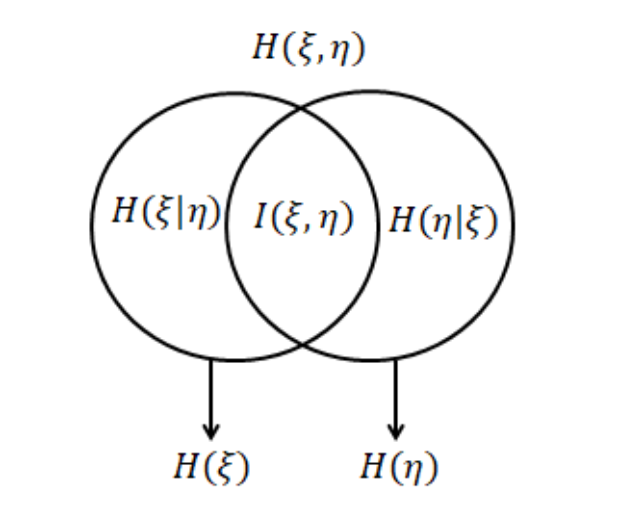
\includegraphics[width=0.4\linewidth]{image/1.png}
\end{figure}






\section{凸函数及其应用}
\subsection{凸函数的定义与判别}
\begin{definition}
     设 $ g(x) $ 是定义在区间 $ (a, b) $ 上的函数,如果对任意的 $ x_{1}, x_{2} \in(a, b) $ 和任意的 $ 0 \leqslant \lambda \leqslant 1 $, 都有
$$
g\left(\lambda x_{1}+(1-\lambda) x_{2}\right) \geqslant \lambda g\left(x_{1}\right)+(1-\lambda) g\left(x_{2}\right)
$$
则称 $ g(x) $ 是 $ (a, b) $ 上的上凸函数,如果等号只有当 $ \lambda=0 $ 或 $ \lambda=1 $或 $ x_{1}=x_{2} $ 时才成立,则称函数 $ g $ 是严格上凸的(若不等式相反称是下凸的).
\end{definition}
\begin{remark}

    (1)如果 $ g $ 是上凸(严格上凸)的,那么 $ -g $ 必是下凸(严格下凸)的;
    
(2) 函数是上凸的, 那么它的函数值总是位于任意弦的上方. 函数是下凸的, 那么它的函数值总是位于任意弦的下面.如$x^2,|x|,e^x,x\log x$等是下凸函数,$\sqrt{x}, \log x$是上凸函数. 注意$ax+b$是上凸也是下凸的.

(3) 像许多信息量,如熵和互信息都具有上凸性.
\end{remark}
\begin{theorem}[判定定理]
    如果函数 $ g $ 在任意处都有非负(正)二阶导数,则函数 $ g $ 是下凸(严格下凸的)
\end{theorem}
\begin{proof}
    函数 $ g $ 在的处的泰勒展开式
$$
g(x)=g\left(x_{0}\right)+g^{\prime}\left(x_{0}\right)\left(x - x_{0}\right)+\frac{1}{2} g^{\prime \prime}\left(x_{*}\right)\left(x-x_{0}\right)^{2}
$$
其中 $ x_*$ 在 $ x $ 与 $ x_{0} $ 之间.

由假设 $ g^{\prime \prime}\left(x_{*}\right) \geqslant 0 $. 则有 $ g(x) \geqslant g\left(x_{0}\right)+g^{\prime}\left(x_{0}\right)\left(x-x_{0}\right) $.令 $ x_{0}=\lambda x_{1}+(1-\lambda) x_{2} $.

当 $ x=x_{1} $ 时有 $ g\left(x_{1}\right) \geqslant g\left(x_{0}\right)+g^{\prime}\left(x_{0}\right)\left(x_{1}-x_{0}\right) $,
而 $ x_{1}-x_{0}=x_{1}-\left[\lambda x_{1}+(1-\lambda) x_{2}\right] =\left(x_{1}-x_{2}\right)(1-\lambda)$,因而有
\begin{equation*}
    g\left(x_{1}\right) \geqslant g\left(x_{0}\right)+g^{\prime}\left(x_{0}\right)(1-\lambda)\left(x_{1}-x_{2}\right) \tag{1}
\end{equation*}

当 $ x=x_{2} $ 时有 $ q\left(x_{2}\right) \geqslant g\left(x_{0}\right)+g^{\prime}\left(x_{0}\right)\left(x_{2}-x_{0}\right) $
而 $ x_{2}-x_{0}=x_{2}-\left[\lambda x_{1}+(1-\lambda) x_{2}\right] =\lambda\left(x_{2}-x_{1}\right)$,因而有
\begin{equation*}
    g\left(x_{2}\right) \geqslant g\left(x_{0}\right)+g^{\prime}\left(x_{0}\right) \lambda\left(x_{2}-x_{1}\right) \tag{2}
\end{equation*}

$$
\begin{aligned}
(1)\times \lambda+(2) \times(1-\lambda) &=\lambda g\left(x_{1}\right)+(1-\lambda) g\left(x_{2}\right) \\& \geqslant \lambda g\left(x_{0}\right)+\lambda g^{\prime}\left(x_{0}\right)(1-\lambda)\left(x_{1}-x_{2}\right) \\
& +(1-\lambda) g\left(x_{0}\right)+\lambda g^{\prime}\left(x_{0}\right)(1-\lambda)\left(x_{2}-x_{1}\right) \\
& =g\left(x_{0}\right)
\end{aligned}
$$
即证下凸性,同理可证严格下凸性.
\end{proof}
易知 $ x \geqslant 0 $ 时, $ x^{2},|x|, e^{x}, x \log x $ 均是严格下凸的 .$ \sqrt{x} $ ,$ \log x $ 是严格上凸的.
如 $ g(x)=x \log x $,有 $ g^{\prime}(x)=1+\log x \quad ,g^{\prime \prime}(x)=\frac{1}{x}>0 $

\subsection{熵函数的凸性}
若$\mathscr{X}$是一个固定的集合,记
$$
 \boldsymbol{\tilde{p}}=\left\{\bar{p}=p(x) \mid x \in \mathscr{X}, p(x) \geqslant 0, \sum_{x \in \mathscr{X}} p(x)=1\right\}
$$
是$\mathscr{X}$上的全体概率分布,那么$H(\bar{p}), H(p \| q)$都是$ \boldsymbol{\tilde{p}}$上的函数.
\begin{theorem}
     (1) 熵函数 $ H(\bar{p}) $ 是 $ \boldsymbol{\tilde{p}} $ 上的上凸函数, 即对 $ \forall 0 \leqslant \lambda \leqslant 1 $, $ \forall \overline{p_{1}}, \overline{p_{2}} \in \boldsymbol{\tilde{p}} $, 总有 $ H\left(\lambda \overline{p_{1}}+(1-\lambda) \overline{p_{2}}\right) \geqslant \lambda H\left(\overline{p_{1}}\right)+(1-\lambda) H\left(\overline{p_{2}}\right) $等号成立的充要条件为 $ \lambda=0 $ 或 1 , 或 $ \overline{p_{1}}=\overline{p_{2}} $;
     
(2) 在 $ q $ 固定时,互熵函数 $ H(p \| q) $ 是 $ p $ 的下凸函数,在 $ p $ 固定时, 互熵函数 $ H(p \| q) $ 是 $ q $ 的下凸函数.
\end{theorem}


\section{连续型随机变量的信息量}
\subsection{连续型随机变量的Shannon熵}

\textbf{1. 连续型随机变量}
\begin{definition}
    设 $ \xi $ 是一个随机变量, 在 $ \mathbb{R}=(-\infty,+\infty) $ (或 $ \mathbb{R} $ 的某个区域 $ \mathscr{X} $ ) 中取值, 称 $ \xi $ 是一个连续型随机变量, 它的概率分布函数定义为
$$
F(x)=P_r\{\xi \leqslant x\}, x \in \mathbb{R}
$$
如果 $ F(x) $ 是连续函数, 那么称随机变量 $ \xi $ 具有连续分布,若 $ F(x) $ 的导数存在, 则 $ f(x)=F^{\prime}(x)=\frac{d F(x)}{d(x)} $ 是 $ \xi $ 的概率分布密度函数
\end{definition}

\begin{remark}
  对于概率分布密度函数 $ f(x) $, 有 $ f(x) \geqslant 0 $, 对 $ \forall x \in \mathscr{X} $,
$$
\int_{-\infty}^{+\infty} f(x) d x=1 \text { . }
$$
\end{remark}

\textbf{2. 连续型随机变量的Shannon 熵}
\begin{definition}
    一个概率密度函数为 $ f(x) $ 的连续型随机变量 $ \xi $ 的熵 $ H(\xi) $ 定义为
$$
H(\xi)=-\int_{\mathscr{X}} f(x) \log f(x) d x .
$$
规定 $ 0 \log 0=0 $, 也称为微分熵
\end{definition}
\begin{example}
     (一致分布) 随机变量 $ \xi $ 在 0 到 $ a $ 之间为一致分布, 于是在 0 到 $ a $ 之间的密度为 $ \frac{1}{a} $, 而在其它处的密度均为 0 , 它的熵为
$$
H(\xi)=-\int_{0}^{a} \frac{1}{a} \log \frac{1}{a} d x=\log a
$$
\end{example}
\begin{remark}
    当 $ a<1 $ 时, $ \log a<0 $, 此时熵为负值, 此时并不代表信息的不确定性的大小, 而在物理学中有其意义.
\end{remark}
\begin{example}
  (指数分布) 设 $ \xi \sim p_{\lambda}(x)=\lambda e^{-\lambda x}, x, \lambda \geqslant 0 $, 它的熵为
$$
\begin{aligned}
H(\xi)  =-\int_{0}^{\infty} p_{\lambda}(x) \log p_{\lambda}(x) d x  &=-\int_{0}^{\infty} \lambda e^{-\lambda x} \log \left(\lambda e^{-\lambda x}\right) d x \\
& =-\lambda \int_{0}^{\infty} e^{-\lambda x}(\log \lambda-\lambda x) d x \\
& =-\lambda \int_{0}^{\infty} e^{-\lambda x}(-\lambda x) d x-\int_{0}^{\infty} \lambda e^{-\lambda x} \log \lambda d x \\
& =\int_{0}^{\infty} e^{-\lambda x}(-\lambda x) d(-\lambda x)-\log \lambda \\
& =1-\log \lambda
\end{aligned}
$$
\end{example}
\begin{example}
  (正态分布) 如果 $ \xi \sim N\left(\mu, \sigma^{2}\right) $ ,其中 $ N\left(\mu, \sigma^{2}\right) $ 表示期望为 $ \mu $,均方为 $ \sigma^{2} $ 的正态分布, 那么它的分布密度为
$$
\phi_{\mu, \sigma^{2}}(x)=\frac{1}{\sqrt{2 \pi \sigma^{2}}} \exp \left(-\frac{(x-\mu)^{2}}{2 \sigma^{2}}\right) .
$$
则它的熵为
$$
\begin{aligned}
H\left(\phi_{\mu, \sigma^{2}}\right)&=-\int \phi_{\mu, \sigma^{2}}(x) \log \phi_{\mu, \sigma^{2}}(x) d x \\
&=-\int \phi_{\mu, \sigma^{2}}(x)\left(-\frac{(x-\mu)^{2}}{2 \sigma^{2}}-\log \sqrt{2 \pi \sigma^{2}}\right) d x \\
&=\frac{E\left\{(\xi-\mu)^{2}\right\}}{2 \sigma^{2}}+\frac{1}{2} \log 2 \pi \sigma^{2} \\
&=\frac{1}{2}+\frac{1}{2} \log 2 \pi \sigma^{2} \\
&=\frac{1}{2} \log 2 \pi e \sigma^{2}
\end{aligned}
$$
\end{example}

\subsection{连续型随机变量的联合熵与条件熵}
$ (\xi, \eta) $ 是一对连续型随机变量, 联合分布为 $ p(x, y) $, 边际分布为 $ p(x), p(y) $, 则有如下定义:

(1) 联合熵 $$ H(\xi, \eta)=-\int p(x, y) \log p(x, y) d x d y $$

(2)条件熵 $$ H(\eta \mid \xi)=-\int p(x, y) \log \frac{p(x, y)}{p(x)} d x d y $$

(3)互信息 $$ I(\xi ; \eta)=\int p(x, y) \log \frac{p(x, y)}{p(x) p(y)} d x d y $$










\section{最大熵原理}
连续型随机变量 $ \xi$, 它的分布密度为$f(x)$, $ H(\xi)=-\displaystyle\int_{\mathscr{X}} f(x) \log f(x) d x $ , $ \xi $ 服从何种概率分布密度函数时, $ H(\xi) $ 最大?

即取合适的概率分布密度函数,使 $ H(\xi) $ 最大.

\subsection{有限区间情形的最大熵(均匀分布时取最大摘)}
设 $ \xi $ 是有限区间 $ \mathscr{X}=(a, b) $ 上取值的随机变量, 约束条件为
$$
\int_{a}^{b} f(x) d x=1
$$
则 $ H(\xi) $ 的最大值为 $ \log (b-a) $, 即 $ H(\xi) \leqslant \log (b-a) $ .

\subsection{半开区间情形的最大熵(指数分布时取最大熵)}

设 $ \xi $ 是在半区间 $ \mathscr{X}=(0, \infty) $ 上取值的随机变量, 约束条件为
$$
\int_{0}^{\infty} f(x) d x=1
$$
其期望固定值为 $ \displaystyle\int_{0}^{\infty} x f(x) d x=\mu>0 $,则 $ H(\xi) $ 的最大值为 $ 1+\log \mu $, 即 $ H(\xi) \leqslant 1+\log \mu,\left(\mu=\frac{1}{\lambda}\right) $ .


\subsection{全区间情形的最大熵(正态分布时取最大熵)}
设 $ \xi $ 是在全区间 $ (-\infty,+\infty) $ 上取值的随机变量,约束条件为
$$
\int_{-\infty}^{+\infty} f(x) d x=1
$$
其期望和方差分别固定为 $ E(\xi)=\mu $ 和 $ D(\xi)=\sigma^{2}>0 $,即 $ \displaystyle\int_{-\infty}^{+\infty} x f(x) d x=\mu $ (数学期望定义),
$$
\int_{-\infty}^{+\infty}(x-\mu)^{2} f(x) d x=\sigma^{2} \text { (方差定义), }
$$
则 $ H(\xi) $ 的最大值为 $ \frac{1}{2} \log \left(2 e \pi \sigma^{2}\right) $,
$$
\text { 即 } H(\xi) \leqslant \frac{1}{2} \log \left(2 e \pi \sigma^{2}\right)
$$
\section{习题课}
\begin{exercise}
     计算 $ H\left(\frac{1}{a}, \frac{1}{a}, \cdots, \frac{1}{a}, \frac{2}{a}, \frac{2}{a}\right) $
\end{exercise}
\begin{solution}
由 $ \Sigma P_{i}=1 $ 知,含 $ (a-4) $ 个 $ \frac{1}{a}$ , 2 个$ \frac{2}{a} $ ,总共$ (a-2) $ 项, 于是
$$
\begin{aligned}
H\left(\frac{1}{a}, \frac{1}{a}, \cdots, \frac{1}{a}, \frac{2}{a}, \frac{2}{a}\right) & =\sum_{i=1}^{a-2} p_{i} \cdot \log \frac{1}{p_{i}} \\
& =\sum_{i=1}^{a-4} \frac{1}{a} \log a+2 \cdot \frac{2}{a} \log \frac{a}{2} \\
& =\frac{a-4}{a} \cdot \log a+\frac{4}{a} \log \frac{a}{2} \\
& =\frac{a-4}{a} \cdot \log a+\frac{4}{a} \log a-\frac{4}{a} \log 2 \\
& =\log a-\frac{4}{a} \log 2
\end{aligned}
$$
\end{solution}

\begin{exercise}
计算 $ H^{\prime}(p) $ ,其中 $ H(p) $ 为熵函数
\end{exercise}
\begin{solution}
$$
\begin{aligned}
H(p) & =-p \log p-(1-p) \log (1-p) \\
H^{\prime}(p) & =-\log p-p \cdot \frac{1}{\ln 2 \cdot p}+\log (1-p)+\frac{1}{1-p} \cdot \frac{1-p}{\ln 2} \\
& =-\log p-\frac{1}{\ln 2}+\log (1-p)+\frac{1}{\ln 2} \\
& =-\log p+\log (1-p) \\
& =\log \frac{1-p}{p}
\end{aligned}
$$
\end{solution}

\begin{exercise}
    设两只口袋中各有 20 个球,第一支口袋中有 10 个白球,5个黑球和5个红球; 第二只口袋中有 8 个白球,8个黑球和4个红球,从每只口袋中各取一个球,试判断哪一个结果的不肯定性更大.
\end{exercise}
 \begin{solution}
 当我们要判断哪个结果的不确定性更大时,可以使用熵来衡量.首先,我们将第一只口袋的球的颜色作为随机变量 $\xi_1$,它的概率分布为:
$$
\xi_1 \sim \left(\begin{array}{ccc}\text{白} & \text{黑} & \text{红} \\ \frac{1}{2} & \frac{1}{4} & \frac{1}{4}\end{array}\right)
$$
其中,$\frac{1}{2}$ 表示白球的概率,$\frac{1}{4}$ 表示黑球的概率,$\frac{1}{4}$ 表示红球的概率.

计算第一只口袋的熵 $H(\xi_1)$:
$$ H\left(\xi_{1}\right)=\frac{1}{2} \log 2+2 \times \frac{1}{4} \log 4=\frac{1}{2}+1=1.5  \text{ bits}
$$
接下来,我们将第二只口袋的球的颜色作为随机变量 $\xi_2$,它的概率分布为:
$$
\xi_2 \sim \left(\begin{array}{ccc}\text{白} & \text{黑} & \text{红} \\ \frac{2}{5} & \frac{2}{5} & \frac{1}{5}\end{array}\right)
$$
其中,$\frac{2}{5}$ 表示白球的概率,$\frac{2}{5}$ 表示黑球的概率,$\frac{1}{5}$ 表示红球的概率.

计算第二只口袋的熵 $H(\xi_2)$:

$$
\begin{aligned}
H\left(\xi_{2}\right) & =\frac{4}{5} \log \frac{5}{2}+\frac{1}{5} \log 5 \\
& =\frac{4}{5}(\log 5-\log 2)+\frac{1}{5} \log 5 \\
& =\frac{4}{5} \log 5+\frac{1}{5} \log 5-\frac{4}{5} \\
& =\log 5-\frac{4}{5} \approx 2.32-0.8 \\
& =1.52 \text { 比特 }
\end{aligned}
$$
比较 $H(\xi_1)$ 和 $H(\xi_2)$ 的值,我们可以得出结论:第二只口袋的结果的不确定性更大,因为它的熵值更大. 
 \end{solution}

 \begin{exercise}
 设 $ \xi $ 和 $ \eta $ 联合分布 $ p(0,0)=\frac{1}{3}, p(0,1)=\frac{1}{3}, p(1,0)=0 $, $ p(1,1)=\frac{1}{3} $, 试求:\\
(1) $ H(\xi), H(\eta) $;\\
(2) $ H(\xi \mid \eta), H(\eta \mid \xi) $\\
(3) $ H(\xi, \eta) $;\\
(4) $ H(\eta)-H(\eta \mid \xi) $;\\
(5) $ I(\xi ; \eta) $;\\
(6) 画出上述各信息之间关系的韦恩图.

 \end{exercise}
 \begin{solution}
 \begin{table}[h]
     \centering
     \resizebox{.3\textwidth}{!}{
     \begin{tabular}{|c|c|c|c|}
\hline\diagbox{$ \eta $}{$ \xi $} & 0 & 1 & $ \sum $ \\
\hline 0 & $ \frac{1}{3} $ & 0 & $ \frac{1}{3} $ \\
\hline 1 & $ \frac{1}{3} $ & $ \frac{1}{3} $ & $ \frac{2}{3} $ \\
\hline$ \sum $ & $ \frac{2}{3} $ & $ \frac{1}{3} $ & 1 \\
\hline
\end{tabular}}
 \end{table}
$$
\xi \sim\left(\begin{array}{cc}
0 & 1 \\
\frac{2}{3} & \frac{1}{3}
\end{array}\right) \quad \eta \sim\left(\begin{array}{cc}
0 & 1 \\
\frac{1}{3} & \frac{2}{3}
\end{array}\right)
$$
(1)
$$
\begin{aligned}
H(\xi) & =\sum_{i=0}^{1} p_{i} \log \frac{1}{p_{i}}=\frac{2}{3} \log \frac{3}{2}+\frac{1}{3} \log 3 \\
& =\frac{2}{3} \log 3-\frac{2}{3} \log 2+\frac{1}{3} \log 3 \\
& =\log 3-\frac{2}{3}
\end{aligned}
$$
$$
\begin{aligned}
H(\eta) & =\sum_{i=0}^{1} p_{i} \log \frac{1}{p_{i}}=\frac{1}{3} \log 3+\frac{2}{3} \log \frac{3}{2} \\
& =\frac{1}{3} \log 3+\frac{2}{3} \log 3-\frac{2}{3} \log 2 \\
& =\log 3-\frac{2}{3}
\end{aligned}
$$
(3)
$$
\begin{aligned}
H(\xi, \eta) & =\sum_{x \in \mathscr{X}} \sum_{x \in \mathscr{Y}} p(x, y) \log \frac{1}{p(x, y)} \\
& =3 \cdot \frac{1}{3} \log 3=\log 3
\end{aligned}
$$
(2)
$$
\begin{aligned}
H(\eta \mid \xi) & =H(\xi, \eta)-H(\xi) \\
& =\log 3-\left(\log 3-\frac{2}{3}\right)=\frac{2}{3} \\
H(\xi \mid \eta) & =H(\xi, \eta)-H(\eta) \\
& =\log 3-\left(\log 3-\frac{2}{3}\right)=\frac{2}{3}
\end{aligned}
$$
(4)
$$
\begin{aligned}
H(\eta)-H(\eta \mid \xi) 
= & \log 3-\frac{2}{3}-\frac{2}{3} \\
= & \log 3-\frac{4}{3}
\end{aligned}
$$
(5)
$$
\begin{aligned}
I(\xi ; \eta) & =H(\xi)+H(\eta)-H(\xi, \eta) \\
& =2\left(\log 3-\frac{2}{3}\right)-\log 3 \\
& =\log 3-\frac{4}{3}
\end{aligned}
$$

 \end{solution}

  \begin{exercise}
设 $ \left\{p_{1}, p_{2}, \cdots, p_{a}\right\} $ 是一个概率分布, 并令 $ q_{m}=p_{m+1}+\cdots+p_{a} $,证明: $ H\left(p_{1}, \cdots, p_{a}\right) \leqslant H\left(p_{1}, \cdots, p_{m}, q_{m}\right)+q_{m} \log (a-m) $, 并指出等号何时成立.
 \end{exercise}
 \begin{solution}
     证明:对于序列 $ p_{1}, \cdots, p_{m}, q_{m} $ ,有$ \sum\limits_{i=1}^{m} p_{i}+q_{m}=1$,其中$q_{m}=\sum\limits_{j=m+1}^{a} p_{j} $, 也即
$$
p_{1}, \cdots, p_{m}, p_{m+1}, \cdots, p_{a} \quad \sum_{i=1}^{a} p_{i}=1\left(i \leqslant m, q_{i}=p_{i}\right)
$$

由熵函数可加性知:
$$
\begin{aligned}
& H\left(p_{1}, \cdots, p_{m}, p_{m+1}, \cdots, p_{a}\right) \\
= & H\left(p_{1}, \cdots, p_{m}, q_{m}\right)+\sum_{i=1}^{m} p_{i} H\left(\frac{p_{i}}{p_{i}}\right)+q_{m} \cdot H\left(\frac{p_{m+1}}{q_{m}}, \cdots, \frac{p_{a}}{q_{m}}\right) \\
\leqslant & H\left(p_{1}, \cdots, p_{m}, q_{m}\right)+q_{m} \log (a-m)(\text { 最大值定理 })
\end{aligned}
$$
$$
\frac{p_{m+1}}{q_{m}}=\cdots=\frac{p_{a}}{q_{m}} \Rightarrow p_{m+1}=\cdots=p_{a} \text { 时等号成立. }
$$
\hrule
证明二: 首先证明 $ H\left(p_{1}, \cdots, p_{a}\right)=H\left(p_{1}, \cdots, p_{m}, q_{m}\right)+q_{m} \cdot H\left(\frac{p_{m+1}}{q_{m}}, \frac{p_{m+2}}{q_{m}}, \cdots, \frac{p_{a}}{q_{m}}\right) $ .
$$
\begin{aligned}
\text { 右边 } & =H\left(p_{1}, \cdots, p_{m}, q_{m}\right)+q_{m} \cdot H\left(\frac{p_{m+1}}{q_{m}}, \frac{p_{m+2}}{q_{m}}, \cdots, \frac{p_{a}}{q_{m}}\right)\\&=\left(-\sum_{i=1}^{m} p_{i} \log p_{i}-q_{m} \log q_{m}\right)-q_{m} \cdot \sum_{i=m+1}^{n} \frac{p_{i}}{q_{m}} \log \frac{p_{i}}{q_{m}} \\
& =-\sum_{i=1}^{m} p_{i} \log p_{i}-q_{m} \log q_{m}-\sum_{i=m+1}^{a} p_{i} \log p_{i}+\log q_{m} \cdot \sum_{i=m+1}^{a} p_{i}\\&=-\sum_{i=1}^{a} p_{i} \log p_{i}=\text { 左边 }
\end{aligned}
$$
由离散最大熵定理有
$$
H\left(\frac{p_{m+1}}{q_{m}}, \frac{p_{m+2}}{q_{m}}, \cdots, \frac{p_{a}}{q_{m}}\right) \leqslant \log (a-m)
$$
因此有
$$
H\left(p_{1}, \cdots, p_{a}\right) \leqslant H\left(p_{1}, \cdots, p_{m}, q_{m}\right)+q_{m} \log (a-m)
$$
等式成立的条件是 $ p_{m+1}=p_{m+2}=\cdots=p_{a}=\dfrac{q_{m}}{a-m} $ 
 \end{solution}

  \begin{exercise}
设 $ \xi $ 是取 $ m $ 个值 $ x_{1}, x_{2}, \cdots, x_{m} $ 的随机变量, $ p\left(\xi=x_{m}\right)=a $,证明: $ H(\xi)=a \log \frac{1}{a}+(1-a) \log \frac{1}{1-a}+(1-a) H(\eta) $, 其中 $ \eta $ 是取 $ m-1 $ 个值 $ x_{1}, x_{2}, \cdots, x_{m-1} $ 的随机变量,
$$
p\left(\eta=x_{j}\right) \stackrel{\text { def }}{=} p\left(\xi=x_{j}\right) /(1-a), 1 \leqslant j \leqslant m-1 .
$$
进一步证
明: $ H(\xi) \leqslant a \log \frac{1}{a}+(1-a) \log \frac{1}{1-a}+(1-a) \log (m-1) $,并确定其中等号成立的条件.
 \end{exercise}
 \begin{solution}
     证明: 由 $ p\left(\eta=x_{j}\right) \stackrel{\text { def }}{=} p\left(\xi=x_{j}\right) /(1-a)  \Rightarrow p\left(\xi=x_{j}\right)=(1-a) p\left(\eta=x_{j}\right), j=1, \cdots, m-1 . $
$$
\begin{aligned}
\text { 故 } H(\xi)&=a \log \frac{1}{a}+\sum_{j=1}^{m-1} p\left(\xi=x_{j}\right) \log \frac{1}{p\left(\xi=x_{j}\right)} \\
&=a \log \frac{1}{a}+\sum_{j=1}^{m-1}(1-a) p\left(\eta=x_{j}\right) \log \frac{1}{(1-a) p\left(\eta=x_{j}\right)}\\
&=a \log \frac{1}{a}+\sum_{j=1}^{m-1}(1-a) p\left(\eta=x_{j}\right) \log \frac{1}{1-a} +\sum_{j=1}^{m-1}(1-a) p\left(\eta=x_{j}\right) \log \frac{1}{p\left(\eta=x_{j}\right)} \\
&=a \log \frac{1}{a}+(1-a) \log \frac{1}{1-a} \sum_{j=1}^{m-1} p\left(\eta=x_{j}\right) +(1-a) \sum_{j=1}^{m-1} p\left(\eta=x_{j}\right) \log \frac{1}{p\left(\eta=x_{j}\right)} \\
&=a \log \frac{1}{a}+(1-a) \log \frac{1}{1-a}+(1-a) H(\eta)
\end{aligned}
$$

根据熵的最大值定理有 $ H(\eta) \leqslant \log (m-1) $等号成立的条件为 $ p\left(\eta=x_{j}\right) $ 为等概率分布 $ p\left(\eta=x_{j}\right)=p\left(\xi=x_{j}\right) /(1-a) $

$$
(m-1) p\left(\eta=x_{j}\right)=1 ,\quad p\left(\eta=x_{j}\right)=\frac{1}{m-1} 
$$
即$$
 p\left(\xi=x_{j}\right)=\frac{1-a}{m-1}, \quad j=1,2, \cdots, m-1 .
$$
 \end{solution}

  \begin{exercise}
设 $ \widetilde{p}=\left\{p_{1}, p_{2}, \cdots, p_{a}\right\} $ 是一个概率分布, 满足 $ p_{1} \geqslant p_{2} $ $ \geqslant \cdots \geqslant p_{a} $, 假设 $ \varepsilon \geqslant 0 $, 使得 $ p_{1}-\varepsilon \geqslant p_{2}+\varepsilon $ 成立, 证明:
$$
H\left(p_{1}, p_{2}, \cdots, p_{a}\right) \leqslant H\left(p_{1}-\varepsilon, p_{2}+\varepsilon, p_{3}, \cdots, p_{a}\right)
$$
 \end{exercise}
 \begin{solution}
     证明: $ H\left(p_{1}, p_{2}, \cdots, p_{a}\right)=-p_{1} \log p_{1}-p_{2} \log p_{2}-\sum\limits_{i=3}^{a} p_{i} \log p_{i} $
$$
\begin{aligned}
& H\left(p_{1}-\varepsilon, p_{2}+\varepsilon, p_{3}, \cdots, p_{a}\right) \\
= & -\left(p_{1}-\varepsilon\right) \log \left(p_{1}-\varepsilon\right)-\left(p_{2}+\varepsilon\right) \log \left(p_{2}+\varepsilon\right)-\sum_{i=3}^{a} p_{i} \log p_{i} \\
= & -p_{1} \log \left(p_{1}-\varepsilon\right)-p_{2} \log \left(p_{2}+\varepsilon\right)-\sum_{i=3}^{a} p_{i} \log p_{i}+\varepsilon \log \frac{p_{1}-\varepsilon}{p_{2}+\varepsilon}
\end{aligned}
$$
由引理\ref{lamma2}知: $ -p_{1} \log \left(p_{1}-\varepsilon\right)-p_{2} \log \left(p_{2}+\varepsilon\right)-\sum\limits_{i=3}^{a} p_{i} \log p_{i} $
$$
\geqslant-p_{1} \log p_{1}-p_{2} \log p_{2}-\sum_{i=3}^{a} p_{i} \log p_{i}
$$
而 $ \varepsilon \log \dfrac{p_{1}-\varepsilon}{p_{2}+\varepsilon} \geqslant 0 $,
故 $ H\left(p_{1}, p_{2}, \cdots, p_{a}\right) \leqslant H\left(p_{1}-\varepsilon, p_{2}+\varepsilon, p_{3}, \cdots, p_{a}\right) $
 \end{solution}

  \begin{exercise}
    设 $ \xi_{1}, \xi_{2} $ 具有相同的分布,但它们不需要是独立的,令 $ \rho=1-\dfrac{H\left(\xi_{1} \mid \xi_{2}\right)}{H\left(\xi_{1}\right)} $\\
(1) 证明: $ \rho=\dfrac{I\left(\xi_{1} ; \xi_{2}\right)}{H\left(\xi_{1}\right)} $;\\
(2) 证明: $ 0 \leqslant \rho \leqslant 1 $;\\
(3)何时 $ \rho=0 $ ?\\
(4)何时 $ \rho=1 $ ?
 \end{exercise}
 \begin{solution}
     证明:
     
(1) $ \rho=1-\dfrac{H\left(\xi_{1} \mid \xi_{2}\right)}{H\left(\xi_{1}\right)}=\dfrac{H\left(\xi_{1}\right)-H\left(\xi_{1} \mid \xi_{2}\right)}{H\left(\xi_{1}\right)}=\dfrac{I\left(\xi_{1} ; \xi_{2}\right)}{H\left(\xi_{1}\right)} $;

(2) 因 $ I\left(\xi_{1} ; \xi_{2}\right) \geqslant 0 ,\quad H\left(\xi_{1}\right) \geqslant H\left(\xi_{1} \mid \xi_{2}\right) $.
所以 $ 0 \leqslant \dfrac{H\left(\xi_{1} \mid \xi_{2}\right)}{H\left(\xi_{1}\right)} \leqslant 1 $
因此 $ 0 \leqslant \rho \leqslant 1 $;

(3) $ \rho=0 $ 即: $ H\left(\xi_{1} \mid \xi_{2}\right)=H\left(\xi_{1}\right) $, 即 $ \xi_{1} $ 与 $ \xi_{2} $ 相互独立;

(4) $ \rho=1 $ 即: $ H\left(\xi_{1} \mid \xi_{2}\right)=0 $, 或 $ I\left(\xi_{1} ; \xi_{2}\right)=H\left(\xi_{1}\right) $.
即 $ \xi_{1}=\xi_{2} $ .
 \end{solution}

  \begin{exercise}
居住某地区的女孩子中有 $ 25 \% $ 是大学生,在女大学生中有 $ 75 \% $是身高为 1.6 米以上的, 而女孩中身高 1.6 米以上的占总数的一半,假如我们得知身高1.6 米以上的某女孩是大学生的消息,问获得多少信息量.
 \end{exercise}
 \begin{solution}
     设事件 $ A $ 为女孩是大学生, 事件 $ B $ 为女孩子身高1.6米以上,知: $ p(A)=0.25, \quad p(B)=0.5, \quad p(B \mid A)=0.75 $.身高1.6米以上的某女孩是大学生这消息表明在事件 $ B $ 的条件下A事件发生, 可得:
$$
p(A \mid B)=\frac{p(A B)}{p(B)}=\frac{p(A) p(B \mid A)}{p(B)}=\frac{0.25 \times 0.75}{0.5}=0.375
$$
因而 $ I(A \mid B)=-\log p(A \mid B)=\log \frac{1}{0.375} $ 比特
 \end{solution}
 \begin{exercise}
设某一彩色电视机分辨率为 $ 500 \times 1000 $, 灰度为 10 , 不同的色彩度为 30 , 求一幅电视画面所含信息量的大小.

 \end{exercise}
 \begin{solution}
     $ \xi_{1} $ 为灰度信源的随机变量
$$
\xi_{1} \sim\left(\begin{array}{cccc}
x_{1} & x_{2} & \cdots & x_{10} \\
\frac{1}{10} & \frac{1}{10} & \cdots & \frac{1}{10}
\end{array}\right)
$$
每个像素灰度含有的信息量为
$ H\left(\xi_{1}\right)=10 \cdot \frac{1}{10} \log 10=\log 10 \approx 3.32 $ 比特则每副电视画面含信息量为
$$
5 \times 10^{5} \times \log 10 \approx 1.66 \times 10^{6} \text { 比特 }
$$

设 $ \xi_{2} $ 为色彩度信源的随机变量
$$
\xi_{2} \sim\left(\begin{array}{cccc}
y_{1} & y_{2} & \cdots & y_{30} \\
\frac{1}{30} & \frac{1}{30} & \cdots & \frac{1}{30}
\end{array}\right)
$$
每个色彩度含有的信息量为 $ H\left(\xi_{2}\right)=\log 30 \approx 4.91 $ 像素亮度与色彩互相独立, 故每个像素含有的信息量为
$$
H\left(\xi_{1}, \xi_{2}\right)=H\left(\xi_{1}\right)+H\left(\xi_{2}\right)=(\log 10+\log 30) \times 5 \times 10^{5} \text { 比特. }
$$
 \end{solution}


 
%\newpage
\section{第一次课后作业}

\begin{tcolorbox}[breakable,colback=blue!5!white,colframe=blue!75!black,
 title= 单选题]
  概率分布 $ \bar{p}=\left\{p_{1}, p_{2}, \cdots, p_{a}\right\} $ 是一个确定性分布 为熵 $ H\left(p_{1}, p_{2}, \cdots, p_{a}\right)=0 $ 的(  ) 条件.

    
(A) 充分条件;
(B) 必要条件;
(C) 充分必要条件;
(D) 既不充分也不必要.
 \tcblower

概率分布 $\bar{p}=\left\{p_{1}, p_{2}, \cdots, p_{a}\right\}$ 是一个确定性分布,即所有的概率都为1或0,因此熵 $H\left(p_{1}, p_{2}, \cdots, p_{a}\right)=0$.

反之,若$H\left(p_{1}, p_{2}, \cdots, p_{a}\right)=0 \text {, 则由 } H\left(p_{1}, p_{2}, \cdots, p_{a}\right) \text { 的 }
$
定义可知, $ \forall i, p_{i} \log _{c} p_{i}=0 $, 或者 $ p_{i}=0 $, 或者 $ \log _{c} p_{i}=0 $, 由于 $ \sum\limits_{i=1}^{a} p_{i}=1, p_{i} \geq 0 $, 存在 $ i $ 使得 $ p_{i}=1 $, 而其它 $ p_{j}=0 $, 因此 $ \bar{p} $ 必为确定型分布.

所以,答案是:(C) 充分必要条件


\end{tcolorbox}


\begin{tcolorbox}[breakable,colback=blue!5!white,colframe=blue!75!black,
 title= 单选题]
 设 $ \xi $ 是一个二元随机变量, 即 $ \mathscr{X}=\{0,1\} $,令 $ p(\xi=1)=p, p(\xi=0)=1-p $. 则有二元熵函数 $ H(p)=p \log _{2} \frac{1}{p}+(1-p) \log _{2} \frac{1}{1-p} $,则当 $ p=$(  ) 时, $ H(p) $ 达到最大值.

(A) $ 0  $ (B) $ \frac{1}{4} $;
(C) $ \frac{1}{2} $;(D) 1 .
  \tcblower
  首先,计算 $ H(p) $ 的导数:
$$
\begin{aligned}
H(p) & =-p \log_2 p-(1-p) \log_2 (1-p) \\
H^{\prime}(p) & =-\log_2 p-p \cdot \frac{1}{\ln 2 \cdot p}+\log_2 (1-p)+\frac{1}{1-p} \cdot \frac{1-p}{\ln 2} \\
& =-\log_2 p-\frac{1}{\ln 2}+\log_2 (1-p)+\frac{1}{\ln 2} \\
& =-\log_2 p+\log_2 (1-p) \\
& =\log_2 \frac{1-p}{p}
\end{aligned}
$$
令导数等于零,解方程 $ \log _{2} \frac{1-p}{p}=0 $,得到 $ p=\frac{1}{2} $.

接下来,我们来验证 $ p=\frac{1}{2} $ 是 $ H(p) $ 的最大值点还是最小值点.我们可以通过二阶导数的符号来判断.计算二阶导数:
$$
\begin{aligned}
\frac{d^{2} H(p)}{d p^{2}} &=\frac{d}{d p}\left[\log _{2} \frac{1-p}{p}\right] \\
&=\frac{1}{p(p-1)\ln 2}
\end{aligned}
$$
当 $ p=\frac{1}{2} $ 时,$ \frac{1}{p(p-1)\ln 2}<0 $,所以 $ p=\frac{1}{2} $ 是 $ H(p) $ 的最大值点.

因此,当 $ p=\frac{1}{2} $ 时,$ H(p) $ 达到最大值.选项 (C) $ \frac{1}{2} $ 是正确答案.
\end{tcolorbox}

\begin{tcolorbox}[breakable,colback=blue!5!white,colframe=blue!75!black,
 title= 单选题]
若 $ H(\xi, \eta)=H(\xi)+H(\eta) $ ,则随机变量 $ \xi $与 $\eta$ 的关系(  ).

A. $ \xi $ 由 $ \eta $ 决定;

B. $ \eta $ 由$ \xi $决定;

C. $ \xi $ 与 $ \eta $ 相互独立.

  \tcblower

当两个随机变量 $\xi$ 和 $\eta$ 相互独立时,它们的联合概率分布可以表示为它们各自的边缘概率分布的乘积,即 $p(\xi, \eta) = p(\xi) \cdot p(\eta)$.根据熵的定义,随机变量的熵可以表示为 $H(\xi) = -\sum\limits_{{X}} p(x) \log p(x)$,其中 $x$ 是随机变量 $\xi$ 的取值.同样地,$H(\eta) = -\sum\limits_{{Y}} p(y) \log p(y)$,其中 $y$ 是随机变量 $\eta$ 的取值.当两个随机变量相互独立时,它们的联合熵可以表示为 $H(\xi, \eta) = -\sum\limits_{X}\sum\limits_{Y} p(x, y) \log p(x, y)$.由于它们相互独立,联合概率分布可以拆分为各自的边缘概率分布的乘积,即 $p(x, y) = p(x) \cdot p(y)$.代入联合熵的定义中,我们有:

$$
\begin{aligned}
H(\xi, \eta) &= -\sum_{X}\sum_{Y} p(x, y) \log p(x, y) \\
&= -\sum_{{X}}\sum_{Y} p(x) \cdot p(y) \log (p(x) \cdot p(y)) \\
&= -\sum_{X}\sum_{Y} p(x) \cdot p(y) (\log p(x) + \log p(y)) \\
&= -\sum_{X}\sum_{Y} p(x) \cdot p(y) \log p(x) - \sum_{X}\sum_{Y} p(x) \cdot p(y) \log p(y) \\
&= -\sum_{X} p(x) \log p(x) - \sum_{Y} p(y) \log p(y) \\
&= H(\xi) + H(\eta)
\end{aligned}
$$

因此,当 $H(\xi, \eta) = H(\xi) + H(\eta)$ 时,可以得出 $\xi$ 和 $\eta$ 是相互独立的.

\end{tcolorbox}



\begin{tcolorbox}[breakable,colback=blue!5!white,colframe=blue!75!black,
 title= 单选题]
$  \mathrm{H}(\xi, \eta)=\mathrm{H}(\xi) $ ,则随机变量 $ \xi $ 与 $ \eta $ 的关系 ( ).

A. $ \xi $ 由 $ \eta $ 决定;

B. $ \xi $ 与相互独立;

C. $ \eta $ 由$ \xi $决定.
  \tcblower

根据题目中的信息 $ \mathrm{H}(\xi, \eta)=\mathrm{H}(\xi) $,这意味着给定 $ \xi $ 的情况下, $ \eta $ 的条件熵为零,即 $ \mathrm{H}(\eta|\xi) = 0 $.这表明在已知 $ \xi $ 的情况下, $ \eta $ 是确定的,因此可以得出结论: $ \eta $ 由 $ \xi $ 决定.因此,答案是 C. $ \eta $ 由 $ \xi $ 决定.

\end{tcolorbox}


\begin{tcolorbox}[breakable,colback=blue!5!white,colframe=blue!75!black,
 title=计算题]
计算 $ H\left(\frac{1}{a}, \frac{1}{a}, \cdots, \frac{1}{a}, \frac{2}{a}, \frac{2}{a}\right) $


 \tcblower
由 $ \Sigma P_{i}=1 $ 知,含 $ (a-4) $ 个 $ \frac{1}{a}$ , 2 个$ \frac{2}{a} $ ,总共$ (a-2) $ 项, 于是
$$
\begin{aligned}
H\left(\frac{1}{a}, \frac{1}{a}, \cdots, \frac{1}{a}, \frac{2}{a}, \frac{2}{a}\right) & =\sum_{i=1}^{a-2} p_{i} \cdot \log \frac{1}{p_{i}} \\
& =\sum_{i=1}^{a-4} \frac{1}{a} \log a+2 \cdot \frac{2}{a} \log \frac{a}{2} \\
& =\frac{a-4}{a} \cdot \log a+\frac{4}{a} \log \frac{a}{2} \\
& =\frac{a-4}{a} \cdot \log a+\frac{4}{a} \log a-\frac{4}{a} \log 2 \\
& =\log a-\frac{4}{a} \log 2
\end{aligned}
$$
\end{tcolorbox}


\begin{tcolorbox}[breakable,colback=blue!5!white,colframe=blue!75!black,
 title=计算题]
设两只口袋中各有20个球,第一支口袋中有10个白球,5个黑球和5 个红球; 第二只口袋中有8个白球, 8 个黑球和 4 个红球,从每只口袋中各取一个球, 试判断哪一个结果的不肯定性更大.


 \tcblower
当我们要判断哪个结果的不确定性更大时,可以使用熵来衡量.
首先,我们将第一只口袋的球的颜色作为随机变量 $\xi_1$,它的概率分布为:
$$
\xi_1 \sim \left(\begin{array}{ccc}\text{白} & \text{黑} & \text{红} \\ \frac{1}{2} & \frac{1}{4} & \frac{1}{4}\end{array}\right)
$$
其中,$\frac{1}{2}$ 表示白球的概率,$\frac{1}{4}$ 表示黑球的概率,$\frac{1}{4}$ 表示红球的概率.

计算第一只口袋的熵 $H(\xi_1)$:
$$ H\left(\xi_{1}\right)=\frac{1}{2} \log 2+2 \times \frac{1}{4} \log 4=\frac{1}{2}+1=1.5  \text{ bits}
$$
接下来,我们将第二只口袋的球的颜色作为随机变量 $\xi_2$,它的概率分布为:
$$
\xi_2 \sim \left(\begin{array}{ccc}\text{白} & \text{黑} & \text{红} \\ \frac{2}{5} & \frac{2}{5} & \frac{1}{5}\end{array}\right)
$$
其中,$\frac{2}{5}$ 表示白球的概率,$\frac{2}{5}$ 表示黑球的概率,$\frac{1}{5}$ 表示红球的概率.

计算第二只口袋的熵 $H(\xi_2)$:

$$
\begin{aligned}
H\left(\xi_{2}\right) & =\frac{4}{5} \log \frac{5}{2}+\frac{1}{5} \log 5 \\
& =\frac{4}{5}(\log 5-\log 2)+\frac{1}{5} \log 5 \\
& =\frac{4}{5} \log 5+\frac{1}{5} \log 5-\frac{4}{5} \\
& =\log 5-\frac{4}{5} \approx 2.32-0.8 \\
& =1.52 \text { bits }
\end{aligned}
$$
比较 $H(\xi_1)$ 和 $H(\xi_2)$ 的值,我们可以得出结论:第二只口袋的结果的不确定性更大,因为它的熵值更大. 
\end{tcolorbox}
\chapter{信源编码}


编码 $ \left\{\begin{array}{l}\text { 信源编码 }\left\{\begin{array}{l}\text { 减少冗余度,即把信源输出符号序列变换为最短的 } \\ \text { 把相关性降低,使各符号尽量独立 } \\ \text { 码字不能改变信源所携带的最低的信息 }\end{array}\right.\\ \text{信道编码}\end{array}\right. $

\begin{figure}[h]
    \centering
    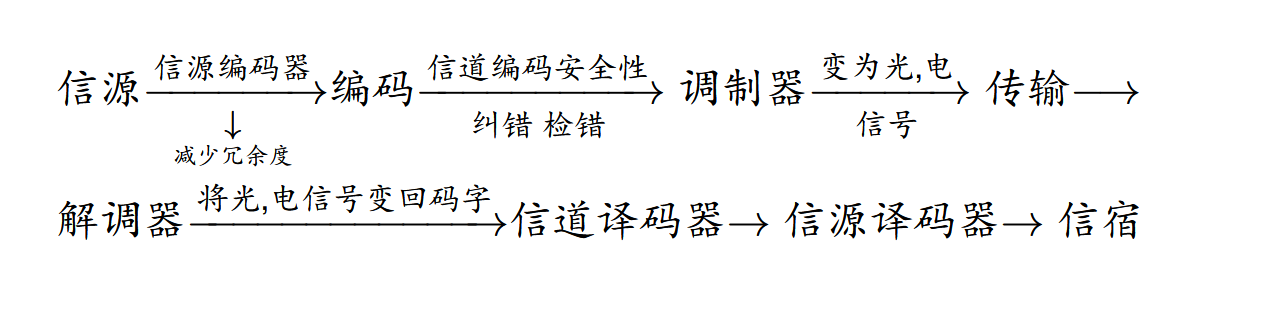
\includegraphics[width=1\linewidth]{image/2.png}
    %\caption{Enter Caption}
\end{figure}

\section{信源编码问题}
\subsection{信源编码}
\begin{definition}
     信源序列: 设 $ \mathscr{S}=\{\mathscr{X}, p(x)\} $ 为信源, 其中 $ \mathscr{X} $ 为信息字母表, $ p(x), x \in \mathscr{X} $ 为消息字母表上的概率分布,将 $ \mathscr{X} $中的信源字母进行分组, 记为 $ x_{1}^{(n)}, x_{2}^{(n)}, \cdots, x_{L}^{(n)} $.其中 $ x_{i}^{(n)}=\left\{x_{i 1}, x_{i 2}, \cdots, x_{i n}\right\}, i=1, \cdots, L, x_{i j} \in X $, $ j=1, \cdots, n $. 每个 $ x_{i}^{(n)} $ 的概率分布记为 $ p_{i}^{(n)} $,记 $ \mathscr{S}^{n}=\left\{\mathscr{X}^{n}, p^{(n)}\left(x^{(n)}\right)\right\} $ 称其为信源序列.
\end{definition}

\begin{remark}

(1)发送消息时通常不是一个一个信源字母进行发送, 而是把它们分组变为信源序列后进行发送, 可以减少发送次数.

(2)例: $ \mathscr{X}=\{0,1\}, p(0)=p, p(1)=1-p $,
$x_{1}^{(3)}=001, x_{2}^{(3)}=111, x_{3}^{(3)}=101 $,
 则  $p_{1}^{(3)}=(p, p, 1-p), p_{2}^{(3)}=(1-p, 1-p, 1-p) ,
p_{3}^{(3)}=(1-p, p, 1-p)$.
于是信源序列为 $ \left\{\mathscr{X}^{3}, p^{(3)}\left(x^{(3)}\right)\right\} $.
\end{remark}


\begin{definition}
    记 $ \mathscr{U} $ 和 $ \mathscr{U}^{m} $ 分别为信道的输入信号字母表和输入信号字母表序列, $ \mathscr{U}^{*}=\bigcup\limits_{m=1}^{\infty} \mathscr{U}^{m} $ 为由全体信号字母串所组成的集合,其中 $ \mathscr{U}^{m} $是全体在 $ \mathscr{U} $ 上取值的 $ m $ 维向量的集合,则称映射 $ f: \mathscr{X}\left(\mathscr{X}^{n}\right) \rightarrow \mathscr{U}^{*} $ 为信源编码 $ f $.
\end{definition}
\begin{remark}

    (1) $ f: \mathscr{X}^{n} \rightarrow \mathscr{U}^{*} $ 即 $ f $ 可把 $ n $ 长的消息序列变为信号序列(可以不等长);
    
(2)信源编码的基本要求是编码运算的可还原性,即可唯一的把码字还原为消息.

(3)编码可还原性的一个必要条件是编码运算 $ f $ 的 $ 1-1 $ 性(显然,后面举例说明 $ 1-1 $ 性是必要条件而不是充要条件)

\end{remark}

\begin{definition}
$ 1-1 $ 码: 如果对于 $ \forall x \neq x^{\prime} \in \mathscr{X} $, 都有 $ f(x) \neq f\left(x^{\prime}\right) $, 则称 $ f $ 是一个1 - 1 编码,也称 $ f $ 满足 $ 1-1 $ 性.
\end{definition}
\begin{remark}
 $ 1-1 $ 码不一定是可还原码,后面举例说明.
\end{remark}

\subsection{定长编码与变长编码}
1.定长编码与变长编码
\begin{definition}
    若编码 $ f: \mathscr{X}^{n} \rightarrow \mathscr{U}^{m} $, 其中 $ m, n $ 是两个固定的正整数, 则称 $ f $ 是一个定长编码, 即把 $ \left(x_{1}, \cdots, x_{n}\right) \rightarrow\left(u_{1}, \cdots, u_{m}\right) $ (码字长度固定)若 $ f: \mathscr{X} \rightarrow \mathscr{U}^{*} $, 称 $ f $ 为变长编码(码字长度不固定)
\end{definition}
2. 扩张编码与唯一可译码
\begin{definition}
    (1)设 $ f: \mathscr{X}\left(\mathscr{X}^{n}\right) \rightarrow \mathscr{U}^{m} $ 定长编码. 记 $ x^{(k n)}=\left(x_{1}^{(n)}, x_{2}^{(n)}, \cdots, x_{k}^{(n)}\right) $, 其中 $ x_{j}^{(n)}=\left(x_{j 1}, \cdots, x_{j n}\right) $ $ j=1,2, \cdots, k $. 对任何的 $ k=1,2,3, \cdots $, 定义
$$
f^{*}\left(x^{(k n)}\right)=\left(f\left(x_{1}^{(n)}\right), f\left(x_{2}^{(n)}\right), \cdots, f\left(x_{k}^{(n)}\right)\right)
$$
则称 $ f^{*} $ 是 $ f $ 的扩张编码. 这时 $ f^{*} $ 是一个从 $ \left(\mathscr{X}^{n}\right)^{*} $ 到 $ \mathscr{U}^{*} $ 的映射.

(2) 设 $ f $ 是 $ \mathscr{X} $ 到 $ \mathscr{U}^{*} $ 的变长码, $ x^{(k)}=\left(x_{1}, x_{2}, \cdots, x_{k}\right) $ 是一个消息字母串, 对任何 $ k=1,2,3, \cdots $, 定义
$$
f^{*}\left(x^{(k)}\right)=\left(f\left(x_{1}\right), f\left(x_{2}\right), \cdots, f\left(x_{k}\right)\right)
$$
称 $ f^{*} $ 是 $ f $ 的扩张编码. 这时 $ f^{*} $ 是一个从 $ \mathscr{X}^{*} $ 到 $ \mathscr{U}^{*} $ 的映射.

(3) 无论是定长编码还是变长编码, 它们的扩张 $ f^{*} $ 都是从 $ \left(\mathscr{X}^{n}\right)^{*} $ (或 $ \mathscr{X}^{*} $ ) 到 $ \mathscr{U}^{*} $ 的映射.如果 $ f^{*} $ 是一个 $ 1-1 $ 映射,那么我们称 $ f $ 是一个唯一可译码(或可还原码).
\end{definition}

3. 唯一可译码与 $ 1-1 $ 码的关系
\begin{theorem}
 (1)无论是定长编码还是变长编码, 唯一可译码必是 $ 1-1 $ 码.\\
(2)如果 $ f $ 是一个 $ 1-1 $ 定长码,那么 $ f $ 是一个唯一可译码.\\
(3)唯一可译的变长码 $ f $ 一定是 $ 1-1 $ 码,反之不然.
\end{theorem}
\begin{proof}
    (1) 用反证法.若 $ f $ 不是 $ 1-1 $ 码, 由扩张编码的定义 $ f^{*} $ 也不是一一映射,与 $ f $ 是唯一可译码矛盾,故 $ f $ 必是 $ 1-1 $ 码.

(2) 证明 $ f $ 是唯一可译码, 只需证明 $ f^{*} $ 是一一映射( $ f $ 是定长码 ) ,即 $ f^{*} $ 是单射.设 $ x^{(k n)} \neq y^{(k n)} $, 那么必有一个 $ j \in\{1,2, \cdots, k\} $ 使 $ x_{j}^{(n)} \neq y_{j}^{(n)} $, 因为 $ f $ 是 $ 1-1 $ 码, 所以必有 $ f\left(x_{j}^{(n)}\right) \neq f\left(y_{j}^{(n)}\right) $, 从而
$$
\left(f\left(x_{1}^{(n)}\right), f\left(x_{2}^{(n)}\right), \cdots, f\left(x_{k}^{(n)}\right)\right) \neq\left(f\left(y_{1}^{(n)}\right), f\left(y_{2}^{(n)}\right), \cdots, f\left(y_{k}^{(n)}\right)\right),
$$
即 $ f^{*}\left(x^{(k n)}\right) \neq f^{*}\left(y^{(k n)}\right), f^{*} $ 是 $ 1-1 $ 映射(单射). 从而 $ f $ 是唯一可译码.

(3) 由(1)知唯一可译的变长码 $ f $ 一定是 $ 1-1 $ 码. 下面举例说明对于变长码来说, $ f $ 是 $ 1-1 $ 码, $ f $ 不一定是唯一可译码,即 $ f^{*} $ 不一定是 $ 1-1 $ 映射.

取 $ \mathscr{X}=\{a, b, c\}, \mathscr{U}=\{0,1\} $, 令 $ f(a)=0, f(b)=01, f(c)=001 $.则 $ f $ 是一个 $ 1-1 $ 变长码,但 $ f $ 不是唯一可译码.

事实上, $ f^{*}(c)=(0,0,1), f^{*}(a, b)=(f(a), f(b))=(0,0,1) $, $ (a, b) \neq c $, 但 $ f^{*}(a, b)=f^{*}(c) $, 因此 $ f^{*} $ 不是 $ \mathscr{X}^{*} $ 到 $ \mathscr{U}^{*} $ 的 $ 1-1 $ 映射,故 $ f $ 不是唯一可译码.
\end{proof}

4. 一些概念

(1)二元码:如果信号字母集 $ \mathscr{U}=\{0,1\} $, 则称相应的码(定长或者变长) 为二元码,称 $ \mathscr{U}_f=\{f(x) \mid x \in \mathscr{X}\} $ 为码元集,记作 $ C=\mathscr{U}_{f}=\left\{c_{1}, c_{2}, \cdots, c_{a}\right\} $,其中 $ c_{i}=f\left(x_{i}\right) $.

(2) 记 $ \ell_{f}(x) $ 为码字 $ f(x) $ 的长度, $ \ell_{i}=\ell_{f}\left(x_{i}\right) $ 为 $ x_{i} $ 对应的码字 $ f\left(x_{i}\right) $ 的长度,此时码元集 $ C=\mathscr{U}_{f}=\left\{u_{i}^{\left(\ell_{i}\right)}, i=1,2, \cdots, a\right\} $,
$$
u_{i}^{\left(\ell_{i}\right)}=\left(u_{i 1}, u_{i 2}, \cdots, u_{i \ell_{i}}\right)=f\left(x_{i}\right), u_{i j} \in \mathscr{U}
$$
此时有 $ C=\left\{c_{1}, c_{2}, \cdots, c_{a}\right\}=\left\{u_{1}^{\left(\ell_{1}\right)}, u_{2}^{\left(\ell_{2}\right)} \cdots, u_{a}^{\left(\ell_{a}\right)}\right\} $,如上例 $ C=\mathscr{U}_{f}=\{0,01,001\}, \ell_{1}=1, \ell_{2}=2, \ell_{3}=3 $,因此有
$$
C=\left\{u_{1}^{(1)}, u_{2}^{(2)}, u_{3}^{(3)}\right\} \text {. }
$$
\subsection{信源变长码的编码问题}

\begin{definition}[变长编码 $ f $ 的平均码长]
    设 $ \mathscr{S}=\{\mathscr{X}, p(x)\} $ 是一个信源, $ f $ 是一个变长编码, 对于 $ \forall x \in \mathscr{X}, f(x) \in \mathscr{U}^{*} $, 记 $ \ell_{f}(x) $ 是 $ f(x) $ 的向量长度, 定义 $$ L(\mathscr{S}, f)=\sum_{x \in \mathscr{X}} p(x) \ell_{f}(x) $$ 为变长编码 $ f $ 的平均码长.
\end{definition}
\begin{remark}
    (1)平均码长小占存储空间少,易于传输.
(2) 平均码长与概率分布密切相关.
\end{remark}

\begin{example}
    考虑信源 $ \mathscr{S}=\left(\begin{array}{cccc}a & b & c & d \\ \frac{2}{17} & \frac{2}{17} & \frac{9}{17} & \frac{4}{17}\end{array}\right) \quad \mathscr{X}=\{a, b, c, d \}$.
    
    $ \mathscr{U}=\{0,1\} $ 是二进制信号字母表, $ f_{1}, f_{2} $ 是两个编码方案, 
    $$ f_{1}: \quad f_{1}(a)=11, \quad f_{1}(b)=0, \quad f_{1}(c)=100, f_{1}(d)=10 $$
    $$ f_{2}: \quad f_{2}(a)=01010, \quad f_{2}(b)=00, \quad f_{2}(c)=10, \quad f_{2}(d)=11 $$

计算它们的平均码长
$$
\begin{aligned}
&L\left(\mathscr{S}, f_{1}\right)=\frac{2}{17} \times 2+\frac{2}{17} \times 1+\frac{9}{17} \times 3+\frac{4}{17} \times 2=\frac{41}{17} \\
&L\left(\mathscr{S}, f_{2}\right)=\frac{2}{17} \times 5+\frac{2}{17} \times 2+\frac{9}{17} \times 2+\frac{4}{17} \times 2=\frac{40}{17}
\end{aligned}
$$
\end{example}

\begin{definition}[变长信源编码问题]
    如果 $ \mathscr{S}=\{\mathscr{X}, p(x)\} $ 是一个给定的信源, 变长信源编码问题是: 求一个唯一可译的变长码 $ f $, 使 $ L(\mathscr{S}, f) $ 最小, 即求唯一可译的变长码 $ f_{0} $, 使得 $ f_{0} $ 相对于其他唯一可译变长码 $ f $,总有
$$
L\left(\mathscr{S}, f_{0}\right) \leq L(\mathscr{S}, f)
$$

这时, 称 $ f_{0} $ 为 $ \mathscr{S} $ 的最优变长码.
\end{definition}
\subsection{信源序列的定长编码问题}

记 $ \mathscr{S}^{n}=\left\{\mathscr{X}^{n}, p^{(n)}\left(x^{(n)}\right)\right\}, n=1,2,3, \cdots $, 是信源序列. $ \mathscr{U} $ 是输入信号字母表, $ \mathscr{U}^{(m)} $ 是 $ \mathscr{U} $ 的 $ m $ 维乘积空间,即 $ \mathscr{U}^{(m)}=\left\{\left(u_{1}, \cdots, u_{m}\right) \mid u_{i} \in \mathscr{U}\right\} $. 定长编码 $ (f, g) $ 分别是 $ f: \mathscr{X}^{n} \rightarrow \mathscr{U}^{m}, \quad g: \mathscr{U}^{m} \rightarrow \mathscr{X}^{n} $

记 $ \xi^{(n)} $ 是由 $ \mathscr{S}^{n} $ 决定的随机变量.


\begin{definition}[编码的平均误差和可达速率]
    (1) 对于固定的信源 $ \mathscr{S}^{n} $, 与编、译码函数 $ (f, g) $, 它们的平均误差为
$$
e_{n}(f, g)=P_{r}\left\{\xi^{(n)} \neq g\left(f\left(\xi^{(n)}\right)\right)\right\}
$$

(2)记 $ C=\mathscr{U}_{f}^{(m)}=\left\{f\left(x^{n}\right) \mid x^{(n)} \in \mathscr{X}^{n}\right\} $ 为定长编码码字的集合,称 $ V_{n}=\left|\mathscr{U}_{f}^{(m)}\right| $ 为编码的信号体积,而称
$$
R_{n}=\frac{1}{n} \log \left(v_{n}\right)=\frac{1}{n} \log \left|\mathscr{U}_{f}^{(m)}\right|
$$
为编码 $ f $ 的码率.
\end{definition}
\begin{remark}

    (1) 记 $ \mathscr{U}=\left\{u_{1}, u_{2}, \cdots, u_{k}\right\} $, 码字长度为 $ m $. 对于 $ u_{i} \in \mathscr{U}, u_{i} $ 能携带的最大信息量为 $ \log _{2} k $.
    
(2)则 $ m $ 长码字所提供的最大信息量为 $ m \log _{2} k $.
\end{remark}



\begin{definition}[信源序列编码的可达速率]
    称 $ R $ 是信源序列 $ \mathscr{S}^{n} $ 的一个可达速率, $ n=1,2, \cdots $, 如果存在一个数列 $ \varepsilon_{n} \rightarrow 0 $, 当 $ n \rightarrow \infty $ 时,存在一组编码序列 $ \left(f^{(n)}, g^{(n)}\right) $ 使得以下条件成立.

(1)对任何 $ n=1,2,3, \cdots, e\left(f^{(n)}, g^{(n)}\right) \leq \varepsilon_{n} \rightarrow 0 $

(2)对任何 $ n=1,2,3, \cdots, R_{n} \leq R\left(1+\varepsilon_{n}\right) \rightarrow R $. 其中 $ R_{n}=\frac{1}{n} \log M_{n}, M_{n}=\left|\mathscr{U}_{f}^{(m)}\right| $.
\end{definition}


可达速率是指对每组编码序列 $ \left(f^{(n)}, g^{(n)}\right) $, 在误差范围内传输的平均信息量, 故定长编码问题是考虑最小可达速率, 即在误差范围内传输的的平均信息量最小值.

\begin{definition}[信源序列的最小可达速率和它的编码问题]
    对已给的信源序列 $ \mathscr{S}^{n} $, 全体可达速率的最小值,称为该信源序列的最小可达速率,信源序列的编码问题就是求它的最小可达速率.(注:每取一组 $ \left(f^{(n)}, g^{(n)}\right) $ 就有一个可达速率,去找所有的最小值)
\end{definition}

\begin{example}
     $ \mathscr{S} $ 是信源, $ \mathscr{X}=\left\{x_{1}, x_{2}, \cdots x_{5}\right\} $ 为信源字母表,对应的概率分布为 $ p_{1}=1-\varepsilon, p_{2}=p_{3}=p_{4}=p_{5}=\frac{\varepsilon}{4} \cdot \mathscr{U}=\{0,1\} $, 利用定长编码, 则码字长度至少为 3 . (否则最多有 4 个码字, 不能建立映射).码字长度为 $ n $ 的二进制编码可以有 $ 2^{n} $ 个不同的码字,$ 4=2^2<5<2^{3}=8 $.

如果采用变长编码,令
$$
f\left(x_{1}\right)=0,\left(f\left(x_{2}\right), f\left(x_{3}\right), f\left(x_{4}\right), f\left(x_{5}\right)\right)=(100,101,110,111)
$$
它的平均码长为
$$
L(\mathscr{S}, f)=(1-\varepsilon)+4 \times \frac{\varepsilon}{4} \times 3=(1-\varepsilon)+3 \varepsilon=1+2 \varepsilon,
$$
只要 $ \varepsilon<1 $, 就会有 $ L(\mathscr{S}, f)=1+2 \varepsilon<3 $. 如果 $ \varepsilon<\frac{1}{2} $, 则有 $ L(\mathscr{S}, f)=1+2 \varepsilon<2 $. 因此利用变长码可以大大压缩信源的编码长度.

$ f $ 是唯一可译码只需验证 $ f^{*} $ 是 $ 1-1 $ 映射(显然).
\end{example}



\section{前缀码和即时码}

变长码的讨论 $ \left\{\begin{array}{l}\text { (1)唯一可译变长码的构造 } \\ \text { (2)平均码长的估计与优化 }\end{array}\right. $

\subsection{唯一可译变长码的构造}
\begin{example}
    考虑一个信源字母表 $ \mathscr{X}=\{a, b, c, d\} $, 它的编码函数为 $ f(a)=0, f(b)=01, f(c)=011, f(d)=0111 $,则码元集 $ C=\{0,01,011,0111\} $, 则码 $ C $ 是唯一可译码.事实上,假设我们收到的码字串为 01101001110010. 注意到每个码字都是以0开始的,故按此规则将码字符串进行分组, 可得到信源字母串为cbadaba.

    再如收到码字符串为 0100111011 , 则可知信源字母串为badc.码 $ C $ 为唯一可译码, 但注意到我们收到的码字串中有码元011, 我们还不能确定它的信源字母, 因为在 011 后面可能出现 0 或 1 , 如果是 0 , 那么就可把011译出为 $ c $, 如果是 1 , 那么就可把0111译出为 $ d $.即译码不是即时的,依赖于它后面的字符,故称这种码为\textbf{非即时码}.
\end{example}

\begin{example}
 考虑信源字母表 $ \mathscr{X}=\{a, b, c, d\} $, 编码函数为 $ f $ :
$$
f(a)=1, f(b)=01, f(c)=001, f(d)=0001,
$$
它的码元集为
$$
C=\{1,01,001,0001\}
$$
它把 1 作为两个码字的分隔号 (以1为结尾), 收到码字串 10010110001101 时, 译为信源字母串acbadab; 又如收到码字串 0010001101 , 译为信源字母串 cdab, 这种码可直接译码, 不用考虑码字符后面出现什么数字, 当我们收到一个字符串时, 就可从左向右读, 只要码元一出现, 我们就可译出相应的信源字母, 这种码我们称为\textbf{即时码}.
\end{example}

\begin{definition}[即时码与非即时码]
    如果在任意的码串中, 从左到右, 只要一个码字出现, 就可唯一译出这个码字所对应的信源字母, 则称这种码为即时码, 否则为非即时码.
\end{definition}
\begin{remark}

    (1)即时码和非即时码均是对唯一可译码而言.
    
(2)唯一可译码不一定是即时码,如第一个例子.
\end{remark}

\begin{definition}[前缀码]
设有两个字符串 $ a^{(k)}=\left(a_{1}, a_{2}, \cdots, a_{k}\right) $, $ b^{\left(k^{\prime}\right)}=\left(b_{1}, b_{2}, \cdots, b_{k^{\prime}}\right) $, 如果 $ k \leq k^{\prime} $, 且有 $ \left(a_{1}, a_{2}, \cdots, a_{k}\right)=\left(b_{1}, b_{2}, \cdots, b_{k}\right) $, 则称 $ a^{(k)} $ 是 $ b^{\left(k^{\prime}\right)} $ 的前缀. 如果码元集 $ C $ 中任何一个码字都不能是另一个码字的前缀,即在码元集 $ C $ 中, 任何一个码元 $ c_{i} $ 都不能是另一个码元 $ c_{j}(i \neq j) $ 的前缀,就称码 $ C $ 为前缀码.
\end{definition}

如上面第二个例.
$$
f(a)=1, f(b)=01, f(c)=001, f(d)=0001,
$$
每个码字都不是另一个码字的前缀.
但第一个例子中. $ f(a)=0, f(b)=01, f(c)=011, f(d)=0111 $, 就不是前缀码. 码元集 $ C=\{0,01,  011,0111\} $.

如何判断一个码元集是否具有前缀性?只要把每个码元按照它们的长度由小到大排列,把每个码元与它后面的码元进行比较,看它与后面的码元的前边部分是否相同即可. 只要能找到有一个码元能与它后面的码元的前边部分相同,那么这种码就不是前缀码,否则就是前缀码. 
\begin{theorem}[即时码与前缀码的关系]
    前缀码一定是即时码, 反之亦然, 即即时码也是前缀码.
\end{theorem}
\begin{proof}
 $ \Leftarrow $ : 假设 $ C $ 是一个码元集, 若 $ \mathrm{C} $ 不是前缀码, 则存在码字 $ c_{i}, C_{j} $,使得 $ c_{i} $ 是 $ c_{j} $ 的前缀, 在一个含有 $ c_{i} $ 的码字串中, 从左到右, 当 $ c_{i} $ 出现时,只有当 $ c_{i} $ 后面出现部分, 连同 $ c_{i} $ 不是 $ c_{j} $ 时才能把 $ c_{i} $ 还原;若 $ c_{i} $以及连同后面部分是 $ c_{j} $ 时, 不能把 $ c_{i} $ 还原, 应该把 $ c_{j} $ 还原, 因此 $ C $ 不是即时码,矛盾.故即时码一定为前缀码.
 
$ \Rightarrow $ : 若 $ C $ 不是即时码, 则从左到右, 出现一个码字 $ c_{i} $, 还原为消息字母时, 依赖于后面的字符串, 即存在另一个码字 $ c_{j} $, 使得 $ c_{i} $ 是 $ c_{j} $ 的前缀, 从而C不是前缀码.
\end{proof}

\subsection{Kraft不等式}

$ \mathscr{S}=\{\mathscr{X}, p(x)\} $ 是信源, $ \mathscr{U} $ 输入信号字母集, $ f: \mathscr{X} \rightarrow \mathscr{U}^{*} $, 考虑即时码存在的条件.

\begin{theorem}[Kraft不等式]
    如果 $ f $ 是一个变长码, 它的码元集为 $ C $, 它的码字长度分别为 $ \left\{\ell_{1}, \ell_{2}, \cdots, \ell_{a}\right\} $, 记 $ r=|\mathscr{U}| $, 如果 $ f $ 是一个即时码, 那么它必满足Kraft 不等式
$$
\sum_{k=1}^{a} \frac{1}{r^{\ell_{k}}} \leq 1 .
$$
反之, 如果有一组数 $ \left\{\ell_{1}, \ell_{2}, \cdots, \ell_{a}\right\} $ 满足Kraft不等式, 那么必存在一个码长为 $ \left\{\ell_{1}, \ell_{2}, \cdots, \ell_{a}\right\} $ 的即时码.
\end{theorem}

\begin{remark}
反之的含义并不是若 $ C=\left\{c_{1}, c_{2}, \cdots, c_{a}\right\}, \ell_{1}, \cdots, \ell_{a} $ 满足 $ \sum\limits_{k=1}^{a} \frac{1}{r^{l_{k}}} \leq 1 $, 则 $ C $ 一定是即时码.
\end{remark}

\begin{proof}
记 $ C=\mathscr{U}_{f}=\left\{u_{1}^{\left(\ell_{1}\right)}, u_{2}^{\left(\ell_{2}\right)}, \cdots, u_{a}^{\left(\ell_{a}\right)}\right\} $ 是一个即时码的码元集,其中它的码字分别为
$$
u_{i}^{\left(\ell_{i}\right)}=\left\{u_{i 1}, u_{i 2}, \cdots, u_{i \ell_{i}}\right\}, i=1,2, \cdots, a
$$
令 $ \ell=\max \left\{\ell_{i} \mid i=1, \cdots, a\right\} $, 对 $ \forall j=1,2, \cdots, a $,记 
$$ \mathscr{U}_{j}=\left\{\left(u_{j}^{\left(\ell_{j}\right)}, z^{\left(\ell-\ell_{j}\right)}\right) \mid z^{\left(\ell-\ell_{j}\right)} \in \mathscr{U}^{\left(\ell-\ell_{j}\right)}\right\} \subseteq \mathscr{U}^{(\ell)} $$
$ \left(\right. $ 因 $ u_{j}^{\left(\ell_{j}\right)} $ 固定, $ z^{\left(\ell-\ell_{j}\right)}=(*, *, \cdots, *), * \in \mathscr{U},|\mathscr{U}|=r $. 每个位置 $ r $种取法)有
$ \left|\mathscr{U}_{j}\right|=r^{\ell-\ell_{j}} $, 且 $ i \neq j $ 时, $ \mathscr{U}_{i} \neq \mathscr{U}_{j}, \mathscr{U}_{i} \cap \mathscr{U}_{j}=\varnothing $

事实上,若 $ \left(u_{i}^{\left(\ell_{i}\right)}, z_{1}^{\left(\ell-\ell_{i}\right)}\right)=\left(u_{j}^{\left(\ell_{j}\right)}, z_{2}^{\left(\ell-\ell_{j}\right)}\right) $, 不妨设 $ \ell_{i} \leq \ell_{j} $,
则 $ u_{i}^{\left(\ell_{i}\right)} $ 是 $ u_{j}^{\left(\ell_{j}\right)} $ 的前缀, 与 $ f $ 是即时码矛盾. 由 $ \mathscr{U}_{j} \subseteq \mathscr{U}^{(\ell)} $ 知则有 $ \bigcup\limits_{j=1}^{a} \mathscr{U}_{j} \subseteq \mathscr{U}^{(\ell)} $
$$
\left|\bigcup_{j=1}^{a} \mathscr{U}_{j}\right| \leq\left|\mathscr{U}^{(\ell)}\right| $$
$$
\left|\bigcup_{j=1}^{a} \mathscr{U}_{j}\right|=\sum_{j=1}^{a}\left|\mathscr{U}_{j}\right|=\sum_{j=1}^{a} r^{\ell-\ell_{j}} ,\quad\left|\mathscr{U}^{(\ell)}\right|=r^{\ell} $$
即 $$ \sum_{j=1}^{a} r^{\ell-\ell_{j}} \leq r^{\ell} \Rightarrow \sum_{j=1}^{a} \frac{1}{r^{\ell_{j}}} \leq 1 $$
\end{proof}

反之, 假设 $ \ell_{1}, \ell_{2}, \cdots, \ell_{a} $ 和 $ r $ 满足Kraft 不等式. 下面证明存在即时码 $ f $, 使它的码字长度为 $ \ell_{1}, \ell_{2}, \cdots, \ell_{a} $. (下面通过例子来说明构造方法).

\begin{example}
    令 $ \mathscr{U}=\{0,1,2\} $, 且 $ \ell_{1}=\ell_{2}=1, \ell_{3}=2, \ell_{4}=\ell_{5}=4, \ell_{6}=5 $,是否可构造出具有上述码字长度的即时码, 若有, 构造出一个这样的码.
$$
\begin{aligned}
\sum_{i=1}^{6} \frac{1}{r^{\ell_{i}}}&=\frac{1}{3}+\frac{1}{3}+\frac{1}{3^{2}}+\frac{1}{3^{4}}+\frac{1}{3^{4}}+\frac{1}{3^{5}} \\
&=\frac{3^{4}+3^{4}+3^{3}+3+3+1}{3^{5}}=\frac{196}{243}<1
\end{aligned}
$$
满足Kraft不等式,故这样的即时码存在. 构造如下: 设 $ \alpha_{i} $ 为码字长度为 $ i $ 的码字个数.
\begin{enumerate}
    \item 挑选码字长度最小的码字. $ \ell_{1}=\ell_{2}=1, \alpha_{1}=2 $
所以取 $ u_{1,1}=0, u_{1,2}=1 $
( $ u_{i, j} $ 长度为 $ i $ 的第 $ j $ 个码字)
    \item $ \ell_{3}=2, \alpha_{2}=1 $, 取长度为 2 的码字不能以 0,1 开头 (为保证是前缀码),故取 $ \left(u_{2,1,1}, u_{2,1,2}\right)=(2,0) $. 长度为 2 的码字的第 1 个分量不能是码字 $ u_{1,1}, u_{1,2} $.
    \item $ \ell_{4}=\ell_{5}=4 $, 这两个码字不能以 0,1 开头,只能以 2 开头.

同时它的前两个分量不能取 $ (2,0) $, 于是可以取
$$
\begin{array}{l}
\left(u_{4,1,1}, u_{4,1,2}, u_{4,1,3}, u_{4,1,4}\right)=(2,1,0,0), \\
\left(u_{4,2,1}, u_{4,2,2}, u_{4,2,3}, u_{4,2,4}\right)=(2,1,0,1) .
\end{array}
$$
    \item 最后再挑选长度为 5 的码字
$$
\left(u_{5,1,1}, u_{5,1,2}, u_{5,1,3}, u_{5,1,4}, u_{5,1,5}\right)=(2,1,1,0,0) \text {. }
$$
\end{enumerate}
最后我们构造出满足即时性的码为
$$\mathscr{U}_f=\{0,1,20,2100,2101,21100\}$$
\end{example}

\begin{remark}

(1) 若 $ \ell_{1}, \ell_{2}, \cdots, \ell_{2} $ 满足 Kraft不等式, 则必存在码字长度为 $ \ell_{1}, \ell_{2}, \cdots, \ell_{a} $ 的即时码. 如果一个码的码字长度满足 Kraft 不等式, 但它不一定是即时码.

如: 考虑二元码 $ C=\{0,11,100,110\} $,码字长度分别为 $ 1,2,3,3 $,因为$|\mathscr{U}|=2$, 我们有
$$
\frac{1}{2}+\frac{1}{2^{2}}+\frac{1}{2^{3}}+\frac{1}{2^{3}}=1,
$$
所以, 它的码字长度满足kraft 不等式.
但这个码并不是即时的(不是前缀码), 因为码字11是码字110的前缀.
但根据 $ 1,2,3 $, 3 可构造一个即时码,如 $ \{0,10,110,111\} $或 $ \{1,01,001,000\} $.

(2)不满足Kraft不等式的码字长度为 $ \ell_{1}, \ell_{2}, \cdots, \ell_{a} $ 的即时码一定不存在.
\end{remark}







\section{信源变长码的编码定理}
这一节讨论最优变长码平均码长的上、下界估计问题.


\subsection{最优变长码平均码长的下界估计}
记 $ \mathscr{S}=\{\mathscr{X}, p(x)\} $ 为信源, 其中 $ \mathscr{X}=\left\{x_{1}, x_{2}, \cdots, x_{a}\right\} $ 是信源字母表, 对应的概率分布为 $ P=\left(p_{1}, p_{2}, \cdots, p_{a}\right) $. 它的编码方案为 $ (C, f) $, 其中 $ C $ 是一个码元集, 简记为 $ C=\left\{c_{1}, c_{2}, \cdots, c_{a}\right\} $, 码字长度分别是 $ \left\{\ell_{1}, \ell_{2}, \cdots, \ell_{a}\right\} $, 这时平均码长为
$$
L(\mathscr{S}, f)=\sum_{i=1}^{a} p_{i} \ell\left(f\left(x_{i}\right)\right)=\sum_{i=1}^{a} p_{i} \ell_{i}
$$

\begin{theorem}
    如果 $ \mathscr{S}=\{\mathscr{X}, p(x)\} $ 是给定信源, $ f $ 是即时码, 那么
$$
H_{r}\left(p_{1}, \cdots, p_{a}\right) \leqslant L(\mathscr{S}, f),
$$
其中 $ H_{r}(\cdot) $ 是取对数 $ r $ 为底的熵函数, 而等号成立的条件是 $ \ell_{i}=-\log _{r} p_{i}$ , 

$r=|\mathscr{U}|, \mathscr{U} $ 为信号字母表.
\end{theorem}
\begin{proof}
    因为 $ f $ 是即时码, 根据Kraft不等式,我们有
$$
q_{0}=\sum_{i=1}^{a} \frac{1}{r^{\ell_{i}}} \leq 1
$$
令 $ q_{i}=\dfrac{1}{\left(q_{0} r^{\ell_{i}}\right)} $, 则有 $ q_{i} \geq 0, i=1, \cdots, a $,
$$
\sum_{i=1}^{a} q_{i}=\sum_{i=1}^{a} \frac{1}{\left(\sum\limits_{k=1}^{a} \frac{1}{r_{k}}\right) r^{\ell_{i}}}=\frac{\sum\limits_{i=1}^{a} \frac{1}{r^{\ell_{i}}}}{\sum\limits_{k=1}^{a} \frac{1}{r^{\ell_{k}}}}=1
$$
结合引理 \ref{lamma2}则有 
$$
\begin{aligned}
H_{r}\left(p_{1}, \cdots, p_{a}\right)=\sum_{i=1}^{a} p_{i} \log _{r} \frac{1}{p_{i}}
&\leq \sum_{i=1}^{a} p_{i} \log _{r} \frac{1}{q_{i}} \quad\left(p_{i}=q_{i} \text { 等号成立 }\right) \\
&=\sum_{i=1}^{a} p_{i} \log _{r}\left(q_{0} r^{\ell_{i}}\right) \\
&=\sum_{i=1}^{a} p_{i} \ell_{i}+\log _{r} q_{0} \quad (q_{0} \leq 1) \\
&\leq \sum_{i=1}^{a} p_{i} \ell_{i}=L(S, f),
\end{aligned}
$$
等号成立的充要条件为 $ p_{i}=q_{i}, q_{0}=1 $. 即 $ p_{i}=\dfrac{1}{r^{\ell_{i}}} $ 或 $ \ell_{i}=-\log _{r} p_{i} $.
\end{proof}
\begin{remark}
    等号成立的条件为 $ \ell_{i}=-\log _{r} p_{i} $. 即要求 $ \ell_{i}=-\log _{r} p_{i} $ 必须是个整数, 而这个条件并不是总能满足, 所以定理中的等号一般不成立.
\end{remark}

\subsection{ 最优变长码平均码长的上界估计}
\begin{theorem}
    对于已给信源 $ \mathscr{S}=\{\mathscr{X}, p(x)\} $, 它的 $ r $ 元最优变长即时码 $ f_{0} $有
$$
L\left(\mathscr{S}, f_{0}\right)<H_{r}\left(p_{1}, \cdots, p_{a}\right)+1
$$
\end{theorem}
\begin{proof}
    记 $ \operatorname{lnt}(z) $ 是 $ z $ 的整数部分, 而
$$
\ln t_{+}(z)=\left\{\begin{array}{ll}
z, & \text { 如果 } z \text { 是整数 } \\
\operatorname{lnt}(z)+1, & \text { 如果 } z \text { 不是整数 }
\end{array}\right.
$$
如果 $ \overline{p}=\left(p_{1}, p_{2}, \cdots, p_{a}\right) $ 是固定信源的概率分布, 那么我们取 $ \ell_{i}=\operatorname{lnt}_{+}\left(-\log _{r} p_{i}\right) $ 大于或等于 $ \log _{r} \frac{1}{p_{i}} $ 的最小正整数. 那么有 $ \log _{r} \frac{1}{p_{i}} \leq \ell_{i}<\log \frac{1}{p_{i}}+1 $, 且由 $ \log _{r} \frac{1}{p_{i}} \leq \ell_{i} $ 可得 $ \frac{1}{p_{i}} \leq r^{\ell_{i}} $, 因此有 $ \frac{1}{r^{\ell_{i}}} \leq p_{i} $ 成立

从而 $ \sum\limits_{i=1}^{a} \frac{1}{r^{\ell_{i}}} \leq \sum\limits_{i=1}^{a} p_{i}=1 $.
即Kraft不等式成立.因此存在码长为 $ \left\{\ell_{1}, \ell_{2}, \cdots, \ell_{a}\right\} $ 的即时码.这时它的平均码长为
$$
\begin{aligned}
L(\mathscr{S}, f) & =\sum_{i=1}^{a} p_{i} \ell_{i} \\
& <\sum_{i=1}^{a} p_{i}\left(\log _{r} \frac{1}{p_{i}}+1\right) \\
& =\sum_{i=1}^{a} p_{i} \log _{r} \frac{1}{p_{i}}+\sum_{i=1}^{a} p_{i} \\
& =H_{r}\left(p_{1}, \cdots, p_{a}\right)+1
\end{aligned}
$$
于是我们找到了一个平均码字长度小于 $ H_{r}\left(p_{1}, \cdots, p_{a}\right)+1 $ 的即时编码方案.

\end{proof}

\begin{theorem}
    定理:对于已给信源 $ \mathscr{S}=\{\mathscr{X}, p(x)\} $, 它的 $ r $ 元最优变长即时码 $ f_{0} $有
$$
H_{r}\left(p_{1}, \cdots, p_{a}\right) \leq L\left(\mathscr{S}, f_{0}\right)<H_{r}\left(p_{1}, \cdots, p_{a}\right)+1
$$
成立.
\end{theorem}










\section{Huffman信源编码算法}
\subsection{Huffman编码的实例分析}
变长最优码就是平均码字长度取最小值的即时码. 本节我们给出一种有效地构造最优编码方案的算法 —— Huffman 编码.

\begin{example}
    已知信源概率分布为 $ \overline{p}=\{0.24,0.20,0.18,0.13,0.10,0.06,0.05,0.03,0.01\} $, 如取信号字母表 $ \mathscr{U}=\{0,1,2,3\} $,求信源的Huffman编码.
\end{example}

Huffman编码方案的主要运算步骤是构造Huffman数据压缩表与Huffman编码表. 它的运算步骤如下.

1. 先构造 Huffman 数据压缩表\\
(1) 首先把概率分布 $ \overline{p} $ 的概率按大小降序排列, 并作为把它们作为 Huffman数据压缩表第 1 列, 该列长度为 $ a=9 $.\\
(2) 把第一列的 3 个最小的概率相加, 得到新的一列概率分布, 重新按降序排列, 成为Huffman数据压缩表中的第三列. 这时第三列的长度为 7 , 相加后的数为 0.09 , 我们用方框标出.\\
(3) 把第三列的 4 个最小的概率相加, 得到新的一列概率分布, 重新按降序排列, 成为Huffman数据压缩表中的第五列. 这时第五列的长度为 4 , 相加后的数为 0.38 , 我们用方框标出.

2. Huffman 数据压缩表构造 Huffman 编码表\\
(1)因Huffman数据压缩表的第五列的概率分布只有 4 个行, 因此它们的编码正好是 $ 0,1,2,3 $. 把这 4 个数填入Huffman 编码表的第六列. 因此, 第六列是一个码
长为 1 的编码.\\
(2) 在第五列中, 带方框的概率为 0.38 , 它对应的第六列的编码为 0 , 而 0.38 是由第三列的 $ 0.13,0.10,0.09,0.06 $ 这 4 个数相加而成. 这样我们构造第三列概率分布的编码为: 第三列的 $ 0.13,0.10,0.09,0.06 $ 这 4 个数的编码是在 0.38 的编码 0 后边延长 1 个数, 它们分别为 $ 00,01,02,03 $. 第三列中 $ 0.24,0.20,0.18 $ 这 3 个数的编码与第五列的编码相同, 仍为 $ 1,2,3 $. 把 $ 0.24,0.20,0.18,$ $0.13,0.10,0.09,0.06 $ 这 7 个数的编码 $ 1,2,3,00,01,02,03 $ 列入Huffman编码表的第四列.\\
(3) 在表的第三列中, 带方框的概率为 0.09 , 它对应的第四列的编码为 02 , 而 0.09 是由第一列的 $ 0.05,0.03,0.01 $ 这 3 个数相加而成. 这样我们构造第一列概率分布的编码为第一列的前 6 个数的编码与第三列所对应的编码相同. 第一列中 $ 0.05,0.03,0.01 $ 这 3 个数的编码是在第 3 列的 0.09 的编码 02 后边延长 1 个数, 因此它们分别为 $ 020,021,022 $. 把第一列 9 个概率的编码列入Huffman编码表的第二列. 最终完成Huffman编码表. 各项计算结果见表 .

以上过程为 Huffman编码方案. 主要原则是概率大的信源字母对应长度短的码字, 概率小的信源字母对应长度大的码字以保证平均码长尽量小.\textbf{频率高的元素使用较短的编码,频率低的元素使用较长的编码.这样做可以减少整体编码的平均长度,从而达到压缩数据的目的.}


\begin{center}
\begin{tabular}{ll||ll||ll}
\hline 概事 & 码 & 概率 & 码 & 概率 & 码 \\
\hline 0.24 & 1 & 0.24 & 1 & \boxed{0.38} & 0 \\
0.20 & 2 & 0.20 & 2 & 0.24 & 1 \\
0.18 & 3 & 0.18 & 3 & 0.20 & 2 \\
0.13 & 00 & 0.13 & 00 & 0.18 & 3 \\
0.10 & 01 & 0.10 & 01 & & \\
0.06 & 03 & \boxed{0.09} & 02 & & \\
0.05 & 020 & 0.06 & 03 & & \\
0.03 & 021 & & & \\
0.01 & 022 & & & & \\
\hline
\end{tabular}
\end{center}

\subsection{Huffman编码的一般算法}
考虑一般情形. 令码字母表为 $ \mathscr{U}=\{0,1, \cdots, r-1\} $. 信源概率分布为 $ \overline{p}=\left(p_{1}, p_{2}, \cdots, p_{a}\right) $. 构造Huffman 编码的步骤:

1. 若 $ a \leqslant r $, 则取 $ f\left(x_{i}\right)=i-1 $ 即可, $ i=1, \cdots, a $

2. 对于 $ a>r $, 我们观察上述例子的编码过程, 知编码表的最后一列序含 $ r $ 个元素. 设编码表为 $ 2 k $ 列,则有第 $ 2 k $ 列序含 $ r $ 个元,第 $ 2 k-2 $ 列序含 $ 2 r-1 $ 个元, $ 2 k-4 $ 列序含 $ 3 r-2 $ 个元, 即是一个以 $ r-1 $ 为公差的等差数列,故编码表中的第 4 列序含 $ (k-1) r-(k-2) $ 个元.第2列序应含 $ k r-(k-1) $ 个元(确定 $ {k} $ 的值)因此: 

(1) 确定 $ {k} $ 的值. $ k r-k+1 \geq a $, 故 $ k \geq \frac{a-1}{r-1} $, 
${k} $ 取 $ \geq \frac{a-1}{r-1} $ 的最小正整数. 故令 $ k=\operatorname{Int}_{+}\left(\frac{a-1}{r-1}\right) $.

(2)确定第1列中应把最后的几个分量相加,再按大小顺序排列,应该为 $ a-[(k-1) r-(k-2)]+1 $ 个分量相加.

(3)从第3列开始每次将最后 $ r $ 个分量相加,并按大小排序放入下一奇数列, 并将相加所得的概率用框标出. 于是得到了 Huffman压缩表.

(4)按例中编码规则去写出编码表即可.

上述算法称为 Huffman编码算法,得到的编码
$
C=\left\{c_{1}, c_{2}, \cdots, c_{a}\right\}
$
称为 Huffman码.

\begin{example}
    设 $ \mathscr{S}=(\mathscr{X}, p(x)), \bar{p}= $ $ \{0.3,0.1,0.1,0.1,0.1,0.06,0.05,0.05,0.05,0.04,0.03,0.02\} $, 试构造 $ \mathscr{S} $ 上的3元Huffman码并求平均码长.

    解: (1) 先确定 $ {k} $ 的值
$$
k=\operatorname{I n t}_{+}\left(\frac{a-1}{r-1}\right)=\frac{11}{2}=6
$$
(2)再确定第1列最后几个分量相加
$$
\begin{array}{l}
a-(k-1) r+k-1 \\
=12-(6-1) \times 3+6-1 \\
=12-15+6-1=2
\end{array}
$$
于是我们构造Huffman编码为
\begin{center}
\begin{tabular}{ll||ll||ll||ll||ll||ll} 
\hline
概率 & 码 & 概率 & 码 & 概率 & 码 &概率 & 码 & 概率 & 码 & 概率 & 码 \\
\hline
0.3 & 1 & 0.3 & 1 & 0.3 & 1 &0.3 & 1 & 0.3 & 1 &$\boxed{0.4} $ & 0 \\
0.1 & 02 & 0.1 & 02 & $ \boxed{0.14} $ & 01 &$ \boxed{0.16} $ & 00 & $ \boxed{0.3} $ & 2 & 0.3 & 1 \\
0.1 & 20 & 0.1 & 20 & 0.1 & 02 &0.14 & 01 & 0.16 & 00 & 0.3 & 2 \\
0.1 & 21 & 0.1 & 21 & 0.1 & 20 &0.1 & 02 & 0.14 & 01  & \\
0.1 & 22 & 0.1 & 22 & 0.1 & 21 &0.1 & 20 & 0.1 & 02 & \\
0.06 & 000 & 0.06 & 000 & 0.1 & 22 &0.1 & 21 & & & \\
0.05 & 001 & 0.05 & 001 & 0.06 & 000 &0.1 & 22 & & & \\
0.05 & 002 & 0.05 & 002 & 0.05 & 001 & & & &\\
0.05 & 010 & 0.05 & 010 & 0.05 & 002 & & & &\\
0.04 & 012 & $\boxed{0.05}$ & 011 & & & & & &\\
0.03 & 0110 & 0.04 & 012 & & & & & &\\
0.02 & 0111 & & & & & & & &\\
\hline
\end{tabular}
\end{center}

$ L(\mathscr{S}, f)=0.3 \times 1+0.4 \times 2+0.25 \times 3+0.05 \times 4=2.05 $.

\end{example}

\begin{example}
  $ \bar{p}=(0.2,0.1,0.1,0.3,0.1,0.2), r=3 $, 求Huffman编码
    
    解: (1) $ k=\operatorname{lnt}_{+}\left(\frac{a-1}{r-1}\right)=\operatorname{Int}_{+}\left(\frac{6-1}{3-1}\right)=3 $
    
(2)确定第1列后几个分量相加 (最后分量相加的个数): $ a-(k-1) r+k-1=6-(3-1) \times 3+3-1=2 $. 于是有
\begin{center}
\begin{tabular}{ll||ll||ll} 
\hline
概率 & 码 & 概率 & 码 & 概率 & 码 \\
\hline
0.3 & 1 & 0.3 & 1 & $ \boxed{0.5} $ & 0 \\
0.2 & 2 & 0.2 & 2 & 0.3 & 1 \\
0.2 & 00 & 0.2 & 00 & 0.2 & 2 \\
0.1 & 02 & $ \boxed{0.2} $ & 01 & & \\
0.1 & 010 & 0.1 & 02 & & \\
0.1 & 011 & & & &\\
\hline
\end{tabular}
\end{center}

\end{example}












\section{Huffman编码性能分析}

本节对由Huffman信源编码算法所产生的Huffman码的性能进行分析.

\subsection{ Huffman编码的前缀性}
\begin{theorem}[Huffman码的前缀性]
    由Huffman编码算法得到的Huffman码是前缀码.
\end{theorem}
\begin{proof}
     由Huffman编码算法  中的各步骤可知, 第 $ 2 k $ 列中各码元各不相同,且第 $ 2 k-2 $ 列中各码元与第 $ 2 k $ 列中码元相同或是某个码元的延伸, 因此第 $ 2 k-2 $ 列中各码元互不相同, 且每个码元不能成为另一码元的前缀.

一般情形,如果第 $ 2 j $ 列中各码元各不相同,且第 $ 2 j-2 $ 列中各码元与第 $ 2 j $ 列中码元相同或是某个码元的延伸,那么第 $ 2 j-2 $ 列中各码元互不相同,且每个码元不能成为另一码元的前缀.

由此递推, 最后得到第一列中各码元互不能成为另一码元的前缀. 由此定理得证.
\end{proof}

\subsection{Huffman编码的最优性}
\begin{theorem}[Huffman码的最优性定理]
    由Huffman算法构造的Huffman码是最优码, 即对固定信源 $ \mathscr{S} $, 如果我们记 $ f_{0} $ 和 $ f $ 分别是Huffman 码与任一前缀码,那么必有
$$
L\left(\mathscr{S}, f_{0}\right) \leq L(\mathscr{S}, f)
$$
\end{theorem}


为证明这个定理我们先做以下讨论. 设 $ \mathscr{S}, \mathscr{S}^{\prime} $ 是两个信源,我们分别记之为
$$
\mathscr{S}=(\mathscr{X}, \overline{p}), \quad \mathscr{S}^{\prime}=\left(\mathscr{X}^{\prime}, \overline{p^{\prime}}\right),
$$
其中
$$
\begin{array}{l}
\mathscr{X}=\left\{x_{1}, x_{2}, \cdots, x_{a}\right\} . \quad \overline{p}=\left(p_{1}, p_{2}, \cdots, p_{a}\right), \\
\mathscr{X}^{\prime}=\left\{x_{1}^{\prime}, x_{2}^{\prime}, \cdots, x_{a}^{\prime}\right\} . \quad \overline{p^{\prime}}=\left(p_{1}^{\prime}, p_{2}^{\prime}, \cdots, p_{a^{\prime}}^{\prime}\right) \text {, } \\
\end{array}
$$
且
$$
p_{1} \geq p_{2} \geq \cdots \geq p_{a}, \quad p_{1}^{\prime} \geq p_{2}^{\prime} \geq \cdots \geq p_{a^{\prime}}^{\prime},
$$

\begin{lemma}
    如果 $ C=\left\{c_{1}, c_{2}, \cdots, c_{a}\right\} $ 是 $ \mathscr{S} $ 的最优前缀码, 那么必有
$$
\ell\left(c_{1}\right) \leq \ell\left(c_{2}\right) \leq \cdots \leq \ell\left(c_{a}\right)
$$
成立
\end{lemma}
\begin{proof}
 由最优码的定义, 若 $ f_{0} $ 是信源 $ \mathscr{S} $ 的最优码, 则
$$
L\left(\mathscr{S}, f_{0}\right)=\sum_{k=1}^{a} p_{k} \ell\left(c_{k}\right)
$$
最小. 若存在 $ j<i $ 使得 $ \ell\left(c_{j}\right)>\ell\left(c_{i}\right) $, 此时
$$
\begin{array}{c}
L\left(\mathscr{S}, f_{0}\right)=\sum\limits_{k=1}^{a} p_{k} \ell\left(c_{k}\right) \\
>p_{1} \ell\left(c_{1}\right)+\cdots+p_{j-1} \ell\left(c_{j-1}\right)+p_{j} \ell\left(c_{i}\right)+p_{j+1} \ell\left(c_{j+1}\right) \\
+\cdots+p_{i} \ell\left(c_{j}\right)+\cdots+p_{a} \ell\left(c_{a}\right)
\end{array}
$$
事实上
$$
p_{j} \ell\left(c_{j}\right)+p_{i} \ell\left(c_{i}\right)-p_{j} \ell\left(c_{i}\right)-p_{i} \ell\left(c_{j}\right)=\left(p_{j}-p_{i}\right)\left(\ell\left(c_{j}\right)-\ell\left(c_{i}\right)\right)>0
$$
从而 $ f_{0} $ 不是最优码.
\end{proof}

\begin{definition}
    设 $ \mathscr{S}, \mathscr{S}^{\prime} $ 是两个信源,如上所记.我们有以下定义.
    
(1) 称 $ \mathscr{S}^{\prime} $ 是 $ \mathscr{S} $ 的 $ r $ Huffman扩张信源, 如果下面两个条件成立.

(i) $ a<a^{\prime} \leq a+r-1 $.

(ii) 对 $ p $ 和 $ p^{\prime} $, 存在一个正数 $ 1 \leq s \leq a $, 满足
$$
\left\{\begin{array}{ll}
p_{j}=p_{j}^{\prime}, & \text {当} j<s \text { 时, } \\
p_{j}=p_{j-1}^{\prime}, & \text {当} s<j<a \text { 时, } \\
p_{j}=\sum\limits_{j=1}^{a^{\prime}-a+1} p_{a+-1} & \text { 当 } j=s \text { 时, }
\end{array}\right.
$$

(2) 如果
$$
C=\left\{c_{1}, c_{2}, \cdots, c_{a}\right\}, \quad C^{\prime}=\left\{c_{1}^{\prime}, c_{2}^{\prime}, \cdots, c_{a^{\prime}}^{\prime}\right\}
$$
分别是 $ \mathscr{S} $ 和 $ \mathscr{S}^{\prime} $ 的编码, 称 $ C^{\prime} $ 是 $ C $ 的 $ r $ Huffman扩张编码, 如果以下两个条件成立.

(i) $ \mathscr{S}^{\prime} $ 是 $ \mathscr{S} $ 的 $ r $ Huffman扩张信源.

(ii) 码元集合 $ C^{\prime} $ 和 $ C $ 满足
$$
\left\{\begin{array}{ll}
c_{j}^{\prime}=c_{j}, & \text { 当 } j<s \text { 时, } \\
c_{j}^{\prime}=c_{j+1}, & \text { 当 } s<j<a \text { 时, }, \\
c_{a+i-1}^{\prime}=\left(c_{s}, i-1\right) & \text { 当 } i=1,2, \cdots, a^{\prime}-a+1 \text { 时. }
\end{array}\right.
$$
\end{definition}

\begin{lemma}
如果 $ C^{\prime} $ 与 $ C $ 分别是 $ \mathscr{S}^{\prime} $ 与 $ \mathscr{S} $ 的编码, $ \mathscr{S} $ 中的消息个数 $ a=k r-k+1 $, 且 $ C^{\prime} $ 是 $ C $ 的 $ r $ Huffman扩张编码, 那么当 $ C $ 是 $ \mathscr{S} $的最优前缀码时, $ C^{\prime} $ 一定是 $ \mathscr{S}^{\prime} $ 最优前缀码.
\end{lemma}

Huffman编码的最优性定理的证明: 该定理的证明由Huffman编码表的定义与第二个引理即得, 因为有以下结论成立.

(1)在Huffman编码表中,如果记它的第 $ 2 j-1 $ 列
$$
\bar{p}_{j}=\left(p_{j i}, p_{j 2}, \cdots, p_{j t_{j}}\right)
$$
为信源 $ \mathscr{S}_{j} $, 而记它的第 $ 2 j $ 列
$$
C_{j}=\left(c_{j i}, c_{j 2}, \cdots, c_{j t_{j}}\right)
$$
为信源 $ \mathscr{S}_{j} $ 的一个编码, 那么 $ \mathscr{S}_{j} $ 是 $ \mathscr{S}_{j+1} $ 的Huffman扩张信源, $ C_{j} $ 是 $ C_{j+1} $ Huffman 扩张(见定义).

(2) 在Huffman扩张编码表的最后两列第 $ 2 k-1,2 k $ 列中,因为码长 $ \ell\left(c_{k i}\right)=1 $, 所以一定是最优前缀码.

(3) 由上面引理的递推法可得在Huffman编码表的 $ 2 j-1,2 j $ 列中, $ C_{j} $ 一定是 $ \mathscr{S}_{j} $ 的最优前缀码. 因此 $ C=C_{1} $ 一定是 $ \mathscr{S}=\mathscr{S}_{1} $ 的最优前缀码.

\begin{example}
$\bar{p}=(0.32,0.19,0.19,0.11,0.10,0.09) ,\quad \mathscr{U}=\{0,1\}$
$$
\begin{array}{l}
k=\operatorname{lnt}_{+}\left(\frac{a-1}{r-1}\right)=\operatorname{Int}_{+}\left(\frac{6-1}{2-1}\right)=5 \\
a=(k-1) r+k-1=6-(5-1) \times 2+5-1=2
\end{array}
$$
\end{example}

编码一:

\begin{center}
\begin{tabular}{ll||ll||ll||ll||ll}
\hline 概率 & 码 & 概率 & 码 & 概率 & 码 & 概率 & 码 & 概率 & 码 \\
\hline 0.32 & 00 & 0.32 & 00 & 0.32 & 00 & \boxed{0.38} & 1 & \boxed{0.62} & 0\\
 0.19 & 10 & 0.19 & 10 & \boxed{0.30} & 01 & 0.32 & 00 & 0.38 & 1 \\
 0.19 & 11 & 0.19 & 11 & 0.19 & 10 & 0.30 & 01 & & \\
 0.11 & 011 & \boxed{0.19} & 010 & 0.19 & 11 & & &  & \\
 0.10 & 0100 & 0.11 & 011 & & & & & & \\
 0.09 & 0101 & & & &  & & & & \\
\hline
\end{tabular}
\end{center}
码字总长度 17,
$$
L\left(\mathscr{S}, f_{1}\right)=4 \times 0.19+3 \times 0.11+2 \times 0.7=2.49 \text {. }
$$

编码二:
\begin{center}
\begin{tabular}{ll||ll||ll||ll||ll}
\hline 概率 & 码 & 概率 & 码 & 概率 & 码 & 概率 & 码 & 概率 & 码 \\
\hline 0.32 & 00 & 0.32 & 00 & 0.32 & 00 & \boxed{0.38} & 1 & \boxed{0.62} & 0\\
 0.19 & 11 & \boxed{0.19} & 10 & \boxed{0.30} & 01 & 0.32 & 00 & 0.38 & 1 \\
 0.19 & 010 & 0.19 & 11 & 0.19 & 10 & 0.30 & 01 & & \\
 0.11 & 011 & 0.19 & 010 & 0.19 & 11 & & &  & \\
 0.10 & 100 & 0.11 & 011 & & & & & & \\
 0.09 & 101 & & & &  & & & & \\
\hline
\end{tabular}
\end{center}

码字总长度 $ 16, L\left(\mathscr{S}, f_{2}\right)=3 \times 0.49+2 \times 0.51=2.49 $.信源固定的最优码的平均码长的定值2.49. 虽编码方法不同, 但平均码长相同.


上面两个表显示的是构造一个二元Huffman 码的过程, 其中 $ r=2 $. 对相等的概率可有不同的排列, 这时所得的Huffman 码可能不同, 但它们都是最优码, 因此它们的平均码长相等.

 对相等的概率可有不同的排列, 这时由Huffman 算法生成的Huffman编码不同. 经过计算可知, 第一个码的总码字长度是 17 , 而第二个码的总码字长度却是 16 , 但它们的平均码字长度都是 2.49 , 这是为前缀码平均码长的最小值.

\section{ 信源定长码的编码定理}

信源定长码的编码问题我们已在3.1节中给出, 现在讨论它的编码定理, 为了简单起见, 我们只讨论无记忆信源的情形.记 $ \mathscr{S}^{n} $ 是一个由 $ \mathscr{S} $ 决定的无记忆信源. 现在讨论它的定长编码问题,求它的最小可达速率.
为证明定长编码定理,我们先给出以下引理.
\begin{lemma}
    $ R $ 是 $ \mathscr{S}^{n} $ 可达速率的充分与必要条件是存在一列 $ \mathscr{X}^{n} $ 的子集 $ \mathscr{X}_{1}^{n} $, 与一正数列 $ \varepsilon_{n} \rightarrow 0 $,使
$$
M_{n}=\left|\mathscr{X}_{1}^{n}\right|<2^{n R\left(1+\varepsilon_{n}\right)}
$$
且
$$
p\left(\mathscr{X}_{1}^{n}\right)=\operatorname{Pr}\left\{\xi^{n} \in \mathscr{X}_{1}^{n}\right\}>1-\varepsilon_{n}
$$
\end{lemma}

引理给出了可达速率的一个充分必要条件, 证明过程中给出了如何构造可达速率的定义中需要的编译码序列 $ \left(f^{(n)}, g^{(n)}\right) $. 利用该引理可证明下面的信源定长码的编码定理.

\begin{theorem}
 设 $ \mathscr{S}^{n} $ 是一个由 $ \mathscr{S} $ 决定的无记忆信源, 即
$$
p\left(x^{(n)}\right)=p\left(x_{1}\right) p\left(x_{2}\right) \cdots p\left(x_{n}\right) \text {, 对 } \forall x^{(n)}=\left(x_{1}, x_{2}, \cdots, x_{n}\right) \in \mathscr{X}^{n} \text {, }
$$
那么它的最小可达速率为
$$
R_{0}=H(\xi)=H\left(p_{1}, p_{2}, \cdots, p_{a}\right),
$$
其中 $ H(\xi) $ 是 $ \xi $ 的熵.
\end{theorem}
该定理不证明,掌握结论.


\section{习题课}
\subsection{基本概念}

1. 信源编码: $ f: \mathscr{X}\left(\right. $ 或 $ \left.\mathscr{X}^{n}\right) \rightarrow \mathscr{U}^{*} $ 的映射称为一个信源编码.

2. 1-1码: $ f $ 是一个信源编码. 若对 $ \forall x, x^{\prime} \in \mathscr{X}, x \neq x^{\prime} $ 都有 $ f(x) \neq f\left(x^{\prime}\right) $,称为 $ f $ 为一个1-1码,或称 $ f $ 具有 1-1性.

3. 扩张编码 (变长和定长)

4. 唯一可译码: 若 $ f $ 的扩张编码 $ f^{*} $ 是 1-1映射,则称 $ f $ 是唯一可译码.

5. 即时码: 如果对于任意一个码字串, 从左到右. 如果码字 $ c_{i} $ 出现就译为其相应的消息字母, 就称这种码为即时码, 否则称为非即时码.

6. 前缀码:设 $ a^{(k)}=\left(a_{1}, a_{2}, \cdots, a_{k}\right), \quad b^{\left(k^{\prime}\right)}=\left(b_{1}, b_{2}, \cdots, b_{k^{\prime}}\right) $若 $ k \leq k^{\prime} $ 且有 $ \left(a_{1}, \cdots, a_{k}\right)=\left(b_{1}, \cdots, b_{k}\right) $, 则称 $ a^{(k)} $ 为 $ \left.b^{(k '}\right) $ 的前缀. 若在一个码中, 任何一个码字都不是另一个码字的前缀, 即任意码字 $ c_{i} $, 都不是 $ c_{j} $ 的前缀, 称这种码为前缀码.

7. 平均码长: $ \mathscr{S}=(\mathscr{X}, p(x)), \bar{p}=\left\{p_{1}, p_{2}, \cdots, p_{a}\right\} $, $ \ell_{f}(x) $ 为码字 $ f(x) $ 的长度, 称 $ L(\mathscr{S}, f)=\sum\limits_{i=1}^{a} p(x) \ell_{f}(x) $ 为 $ f $ 的平均码长.


\subsection{编码问题与基本结论}

\textbf{1. 变长码的编码问题}

信源固定,构造变长即时码 $ f_{0} $, 使得对任意变长即时码 $ f $ 有
$$
L\left(\mathscr{S}, f_{0}\right) \leq L(\mathscr{S}, f)
$$
此时,称 $ f_{0} $ 为最优变长即时码.

最优码构造方法: Huffman编码算法.

\textbf{2. 定长编码(信源序列)的编码问题}

$ \mathscr{S}^{n}=\left(\mathscr{X}^{n}, p^{(n)}\left(x^{(n)}\right)\right), \quad $ 求最小可达速率.

信源定长码的编码定理:设 $ \mathscr{S}^{n} $ 是一个由 $ \mathscr{S} $ 决定的无记忆信源, 那么它的最小可达速率为
$$
R_{0}=H(\xi)=H\left(p_{1}, p_{2}, \cdots, p_{a}\right),
$$
其中 $ H(\xi) $ 是 $ \xi $ 的熵.

\textbf{3.Kraft不等式(即时码存在的必要条件)}
$$
\sum_{k=1}^{a} \frac{1}{r^{\ell_{k}}} \leq 1 \quad C=\left\{c_{1}, c_{2}, \cdots, c_{a}\right\}
$$
$ \ell_{1}, \ell_{2}, \cdots, \ell_{a} $ 为码字的长度, $ r=|\mathscr{U}| $.
反之, 若 $ \left\{\ell_{1}, \ell_{2}, \cdots, \ell_{a}\right\} $ 满足上式, 则一定存在以 $ \ell_{1}, \ell_{2}, \cdots, \ell_{a} $ 为码字长度的即时码(构造方法).

\textbf{4.满足Kraft不等式的码不一定是即时码,反例需知道.}

\textbf{5. 最优变长码平均码长的上、下界}

定理:对于已给信源 $ \mathscr{S}=\{\mathscr{X}, p(x)\} $, 它的 $ r $ 元最优变长即时码 $ f_{0} $ 有
$$
H_{r}\left(p_{1}, \cdots, p_{a}\right) \leq L\left(\mathscr{S}, f_{0}\right)<H_{r}\left(p_{1}, \cdots, p_{a}\right)+1
$$
成立.

\subsection{课后习题}
\begin{exercise}
下面的码是否是即时码? 是否是唯一可译码?\\
(1) $ C=\{0,10,1100,1101,1110,1111\} $.\\
(2) $ C=\{0,10,110,1110,1011,1101\} $.
\end{exercise}
\begin{solution}
 (1) C 是前缀码, 故是即时码, 从而是唯一可译码.
 
(2) C不是前缀码, 因为码字10是码字1011的前缀, 故C不是即时码.C不是唯一可译码.
字符串
$$
\frac{0}{a} \frac{10}{b} \frac{110}{c} \frac{1110}{d} \frac{1011}{e} \frac{1101}{\mathrm{f}} $$
$$
\frac{0}{a} \frac{1011}{e} \frac{0}{a} \frac{1110}{d} \frac{1011}{e} \frac{1101}{\mathrm{f}}
$$
同一字符串的还原消息为两个, 不是唯一可译码.
\end{solution}


\begin{exercise}
 判断是否存在即时码具有以下的基数和码字长度, 如果有, 试构造出一个这样的码.\\
(1) $ r=2 $, 长度: 1,3,3,3,4,4.\\
(2) $ r=3 $ ,长度: 1, 1,2,2,3,3,3.\\
(3) $ r=5 $, 长度: $ 1,1,1,1,1,8,9 $.

\end{exercise}
\begin{solution}
(1) $ \frac{1}{2}+3 \times \frac{1}{2^{3}}+2 \times \frac{1}{2^{4}}=1 $,故满足Kraft不等式. 即时码存在.
$$
\begin{array}{lllll}
u_{1,1}=0 & 0 & & &\\
u_{3,1,1}=1 & u_{3,1,2}=0 & u_{3,1,3}=0 & (1,0,0) &\\
u_{3,2,1}=1 & u_{3,2,2}=0 & u_{3,2,3}=1 & (1,0,1) &\\
u_{3,3,1}=1 & u_{3,3,2}=1 & u_{3,3,3}=0 & (1,1,0) &\\
u_{4,1,1}=1 & u_{4,1,2}=1 & u_{4,1,3}=1 & u_{4,1,4}=0 & (1,1,1,0)\\
u_{4,2,1}=1 & u_{4,2,2}=1 & u_{4,2,3}=1 & u_{4,2,4}=1& (1,1,1,1)
\end{array}
$$
故此即时码为
$$
\{0,100,101,110,1110,1111)\}
$$

(2)$ 2 \times \frac{1}{3}+2 \times \frac{1}{3^{2}}+3 \times \frac{1}{3^{3}}=1 $ 故满足 Kraft 不等式, 即时码存在.
$$
u_{1,1}=0 \quad u_{1,2}=1 \quad 0,1
$$
$$
\begin{array}{llrl}
u_{2,1,1}=2 & u_{2,1,2}=0 & (2,0) & \\
u_{2,2,1}=2 & u_{2,2,2}=1 & (2,1) & \\
u_{3,1,1}=2 & u_{3,1,2}=2 & u_{3,1,3}=0 & (2,2,0) \\
u_{3,2,1}=2 & u_{3,2,2}=2 & u_{3,2,3}=1 & (2,2,1) \\
u_{3,3,1}=2 & u_{3,3,2}=2 & u_{3,3,3}=2 & (2,2,2)
\end{array}
$$

故此即时码为
$$
\{0,1,20,21,220,221,222\}
$$

(3)$ 5 \times \frac{1}{5}+\frac{1}{5^{8}}+\frac{1}{5^{9}}>1 $, 故这样的即时码不存在.
\end{solution}


\begin{exercise}
在证明 Kraft不等式中,我们说
$$
\frac{\alpha_{1}}{r}+\frac{\alpha_{2}}{r^{2}}+\cdots+\frac{\alpha_{n}}{r^{n}} \leq 1
$$
等价于Kraft不等式.证明这个结果.
\end{exercise}
\begin{solution}
令 $ \alpha_{j} $ 表示 $ \ell_{i}=j $ 的 $ i $ 的个数, 即长度为 $ j $ 的码字个数为 $ \alpha_{j} $ 个, 故长度为 1 的个数为 $ \alpha_{1} $ 个, 长度为 2 的个数为 $ \alpha_{2} $ 个, $ \cdots $, 长度为 $ n $ 的个数为 $ \alpha_{n} $ 个.
$$
\begin{aligned}
\sum_{i=1}^{n} \frac{1}{r^{\ell_{i}}} & =\alpha_{1} \cdot \frac{1}{r^{1}}+\alpha_{2} \cdot \frac{1}{r^{2}}+\cdots+\alpha_{j} \cdot \frac{1}{r^{j}}+\cdots+\alpha_{n} \cdot \frac{1}{r^{n}} \\
& =\sum_{i=1}^{n} \frac{\alpha_{i}}{r^{i}} \leq 1
\end{aligned}
$$
\end{solution}


\begin{exercise}
令 $ C $ 是一个即时码, 试证明下列命题等价.\\
(1) $ C $ 是最大即时码, 即没有码字能够添入 $ C $ 中而令 $ C $ 仍保持即时性.\\
(2) 任意码元素的有限串都是某个码字串的前缀.\\
(3)Kraft不等式中的等号成立.
\end{exercise}
\begin{solution}
只证明 $ (1) \Longleftrightarrow(3) $.

$ \Leftarrow $ : 先证明若 C不是最大即时码, 则Kraft不等式中等号不成立.若 $ C $ 不是最大即时码, 则在码 $ C $ 中可至少添入一个码字, 成为一个新的即时码 $ C_{1} $, 假设 $ C=\left\{c_{1}, c_{2}, \cdots, c_{a}\right\}, c_{i} $ 的码长为 $ \ell_{i} $, $ i=1, \cdots, a $, 设添入的码字为 $ C_{a+1} $, 长度为 $ \ell_{a+1} $, 因 $ C_{1} $ 仍为即时码, 故有
$$
\sum_{i=1}^{a+1} \frac{1}{r^{\ell_{i}}}=\sum_{i=1}^{a} \frac{1}{r^{\ell_{i}}}+\frac{1}{r^{\ell_{a}+1}} \leq 1
$$
从而有 $ \sum\limits_{i=1}^{a} \frac{1}{r^{\ell_{i}}}<1 $. 故 Kraft不等式中等号不成立.

$ \Rightarrow $ : 若Kraft不等式中等号不成立, 令 $ C=\left\{c_{1}, c_{2}, \cdots, c_{a}\right\} $, 对应码字长为 $ \left\{\ell_{1}, \ell_{2}, \cdots, \ell_{a}\right\} $. 此时有$\sum\limits_{k=1}^{a} \frac{1}{r^{\ell_{k}}}<1$
$.
\text { 令 } \ell=\operatorname{lnt}\left(\log _{r}\left(1-\sum\limits_{k=1}^{a} \frac{1}{r^{\ell_{k}}}\right)\right)+1$,
则有 $ \sum\limits_{k=1}^{a} \frac{1}{r^{\ell_{k}}}+\frac{1}{r^{\ell}} \leq 1 $ 故 $ \left\{\ell_{1}, \ell_{2}, \cdots, \ell_{a}, \ell\right\} $ 满足 $ \operatorname{Kraft} $ 不等式于是可构造即时码 $ C^{\prime}=\left\{c_{1}, c_{2}, \cdots, c_{a}, c^{\prime}\right\} $, 与 $ C $ 是最大即时码矛盾.
\end{solution}


\begin{exercise}
 对下面给定的概率分布和基数, 找出一个Huffman编码, 并求平均码长.
$$
p=\{0.3,0.1,0.1,0.1,0.1,0.06,0.05,0.05,0.05,0.04,0.03,0.02\},
\quad r=2 .
$$
\end{exercise}
\begin{solution}
(1) 先确定 ${k} $ 的值.
$$
k=\operatorname{I n t}_{+}\left(\frac{a-1}{r-1}\right)=\frac{11}{1}=11 .
$$
(2)再确定第1列最后几个分量相加.
$$
\begin{array}{l}
a-(k-1) r+k-1 \\
=12-(11-1) \times 2+11-1=2 .
\end{array}
$$
于是我们构造Huffman编码为
\begin{center}
\begin{tabular}{ll||ll||ll||ll||ll||ll} 
\hline
概率 & 码 & 概率 & 码 & 概率 & 码 &概率 & 码 & 概率 & 码 & 概率 & 码 \\
\hline
0.3 & 00 & 0.3 & 00 & 0.3 & 00 &0.3 & 00 & 0.3 & 00 & 0.3 & 00 \\
0.1 & 111 & 0.1 & 111 & 0.1 & 111 &$ \boxed{0.1} $ & 110 & $ \boxed{0.11} $ & 011 & $ \boxed{0.19} $ & 010 \\
0.1 & 100 & 0.1 & 100 & 0.1 & 100 &0.1 & 111 & 0.1 & 110 & 0.11 & 011 \\
0.1 & 101 & 0.1 & 101 & 0.1 & 101 &0.1 & 100 & 0.1 & 111 & 0.1 & 110 \\
0.1 & 0100 & 0.1 & 0100 & 0.1 & 0100 &0.1 & 101 & 0.1 & 100 & 0.1 & 111 \\
0.06 & 0110 & 0.06 & 0110 & $ \boxed{0.09} $ & 0101 &0.1 & 0100 & 0.1 & 101 & 0.1 & 100 \\
0.05 & 1100 & $ \boxed{0.05} $ & 0111 & 0.06 & 0110 &0.09 & 0101 & 0.1 & 0100 & 0.1 & 101 \\
0.05 & 1101 & 0.05 & 1100 & 0.05 & 0111 &0.06 & 0110 & 0.09 & 0101 & & \\
0.05 & 01010 & 0.05 & 1101 & 0,05 & 1100 &0.05 & 0111 & & & &\\
0.04 & 01011 & 0.05 & 01010 & 0.05 & 1101 & & & & & &\\
0.03 & 01110 & 0.04 & 01011 & & & & & & & &\\
0.02 & 01111 & & & & & & & & &\\
\hline
\hline
概率 & 码 & 概率 & 码 & 概率 & 码 &概率 & 码 & 概率 & 码 & & \\
\hline
0.3 & 00 & 0.3 & 00 & 0.3 & 00 &0.4 & 1 & $ \boxed{0.6} $ & 0 & &\\
0.2 & 10 & 0.2 & 10 & $ \boxed{0.3} $ & 01 &0.3 & 00 & 0.4 & 1 & & \\
0.19 & 010$\quad$ & $ \boxed{0.2} $ & 11 & 0.2 & 10 &0.3 & 01 & & & & \\
0.11 & 011 & 0.19 & 010$\quad$ & 0.2 & 11 & & & & & & \\
0.1 & 110 & 0.11 & 011$\quad$ & & & & & & &\\
0.1 & 111 & & & & & & & & & &\\
\hline
\end{tabular}
\end{center}
$$ L(\mathscr{S}, f)=0.14 \times 5+0.26 \times 4+0.3 \times 3+0.3 \times 2=3.24 $$
\end{solution}


\newpage
\begin{mdframed}[frametitle={等价证明}, frametitlerule=true, frametitlebackgroundcolor=yellow!20]

练习题等价命题的证明:

 \textbf{从 (1) 到 (2):}假设 $C$ 是最大即时码,意味着不能向 $C$ 添加更多的码字而保持其即时性.我们需要证明,任意码元素的有限串都是某个码字串的前缀.

由于 $C$ 是最大即时码,如果存在一个码元素的串,它不是任何码字串的前缀,那么我们可以将这个串作为一个新的码字添加到 $C$ 中,而不违反即时性.这与 $C$ 是最大即时码的假设矛盾.因此,任意码元素的有限串必须是某个码字串的前缀.

 \textbf{从 (2) 到 (3):}假设任意码元素的有限串都是某个码字串的前缀.这意味着码字集覆盖了所有可能的码元组合,形成了一种“完整”的编码系统,没有未被利用的“空间”.

Kraft不等式表达了对于长度可变的即时码,其码字长度的集合 $\{l_1, l_2, \ldots, l_n\}$ 必须满足以下条件:
\[
\sum_{i=1}^{n} r^{-l_i} \leq 1
\]
如果任意码元素的有限串都是某个码字串的前缀,这意味着编码系统利用了所有可用的编码“空间”,不留下任何“空隙”.因此,Kraft不等式中的等号必须成立,否则还有“空间”可以添加更多的码字而不违反即时性,这与假设矛盾.

\textbf{ 从 (3) 到 (1):}假设Kraft不等式中的等号成立,即

\[
\sum_{i=1}^{n} r^{-l_i} = 1
\]

这表明编码系统完美地匹配了编码空间的容量,没有未被利用的部分.在这种情况下,不能添加更多的码字而不增加现有码字的长度,因为这将违反Kraft不等式,导致总和超过1.因此,如果Kraft不等式中的等号成立,那么 $C$ 必须是最大即时码,因为没有余地添加更多的码字而保持即时性.
\end{mdframed}









\chapter{信道编码定理}

信道编码的目的:在信源编码的基础上,增加一些适量的冗余信息, 保证信号的安全传输, 最终考虑在保证传输质量的前提下, 最多传输多少数量的信号(信道容量).

\section{信道编码问题}
信道编码问题 $ \left\{\begin{array}{l}\text { 线路编码(变信号) } \\ \text { 差错控制编码(信息论主要讨论的问题) }\end{array}\right. $

\subsection*{信道的分类}
离散信道:输入输出均为离散事件集.

连续信道: 输入输出空间均为连续事件集.

半连续信道: 输入和输出一个是离散的, 一个是连续的.

\subsection*{信道的概率统计模型(表示参数)}
信道的主要参数为转移概率 $ p(v \mid u) $

信道由输入信号集合 $ \mathscr{U} $, 输出信号集合 $ \mathscr{V} $, 及转移概率 $ p(v \mid u) $ 构成.

\begin{remark}
     $ p(v \mid u) $ 转移概率: 当输入信号字母是 $ u $ 时, 输出信号字母为 $ v $的概率. 因此 $ p(v \mid u) \geq 0, \sum\limits_{v \in \mathscr{V}} p(v \mid u)=1 $, 对 $ \forall u \in \mathscr{U}, v \in \mathscr{V} $.信道记为 $ \mathscr{C}=\{\mathscr{U}, p(v \mid u), \mathscr{V}\} $.
\end{remark}


\subsection{通信系统的编码误差}

通信系统 $ \mathscr{E} $ 与编码 $ (f, g) $ 给定后, 输入消息, 输入信号, 输出信号与输出消息的随机变量 $ (\widetilde{\xi}, \xi, \eta, \widetilde{\eta}) $ 也确定,我们称 $$ e(f, g)=P_{r}\{\widetilde{\xi} \neq \widetilde{\eta}\} $$ 为通信系统 $ \mathscr{E}(f, g) $ 所产生的编码误差.

\begin{example}\label{example:4.1.1}
    一个简单的通信系统 $ \mathscr{E} $ 给定如下. 取 $ \mathscr{S} $ 和 $ \mathscr{C} $ 都是四元信源与信道. 这时取 $$ \mathscr{X}=\mathscr{U}=\mathscr{V}=\mathscr{Y}=\{0,1,2,3\} $$它们的信源分布概率为 $$ p(0)=p(1)=p(2)=p(3)=0.25 $$ 信道的转移概率 $ p(v \mid u) $ 为
\begin{center}
\begin{tabular}{c|cccc}
$ u \backslash v $ & 0 & 1 & 2 & 3 \\
\hline
0 & 0.64 & 0.16 & 0.16 & 0.04 \\
1 & 0.16 & 0.64 & 0.04 & 0.16 \\
2 & 0.16 & 0.04 & 0.64 & 0.16 \\
3 & 0.04 & 0.16 & 0.16 & 0.64
\end{tabular}
\end{center}

我们取编码 $ (f, g) $ 为 $ f(x)=x, g(v)=v, x, v=0,1,2,3 $
$$ f: \mathscr{X} \longrightarrow \mathscr{U} \quad \mathscr{U} \xrightarrow{\text { 信道传输 }} \mathscr{V} \quad g: \mathscr{V} \longrightarrow \mathscr{Y} $$
这时 $ (\overline{\xi}, \xi, \eta, \overline{\eta}) $ 的联合概率分布为
$$
p(x, u, v, y)=\left\{\begin{array}{ll}
\frac{1}{4}, & \text { 如果 } x=u, v=y, \\
0, & \text { 否则. }
\end{array}\right.
$$
则此通信系统的编码误差为
$$
\begin{aligned}
e(f, g)= & p(0) P_{r}(0 \neq y)+p(1) P_{r}(1 \neq y)+p(2) P_{r}(2 \neq y)+p(3) P_{r}(3 \neq y) \\
= & 0.25 \times(0.16+0.16+0.04)+0.25 \times(0.16+0.04+0.16)+0.25 \times \\
& (0.16+0.04+0.16)+0.25 \times(0.04+0.16+0.16) \\
= & 0.16+0.16+0.04=0.36
\end{aligned}
$$
误差率达到 $ 36 \% $, 无法使用.
\end{example}
从这个例子中可以看出, 如果改变它的编码, 也不会降低它的编码误差. 一个通信系统如果它的传递误差达到 $ 36 \% $, 那么这个近信系统实际上是无法使用的. 因为改变它的编码方式, 不能降低它的编码误差, 因此如何提高通信系统的通信质量是首先要考虑的问题.

\begin{example}\label{example:4.1.2}
    为了在信道不变的条件下提高通信系统 $ \mathscr{E} $ 的通信质量, 我们减少信源的传输消息数, 如取
$$
\mathscr{X}=\mathscr{Y}=\{0,1\}, \quad p(0)=p(1)=0.5,
$$
而信道与例 \ref{example:4.1.1}相同. 如取编码方案为
$$
f(0)=0, f(1)=3, \quad g(0)=g(1)=0, \quad g(2)=g(3)=1,
$$
那么我们计算它的编码误差为
$$
e(f, g)=0.5 \times(0.16+0.04)+0.5 \times(0.16+0.04)=0.2 .
$$
\end{example}

由例 \ref{example:4.1.1} 和例 \ref{example:4.1.2} 可知, 在信道不变的条件下, 减少信源的传输消息数可以提高通信质量. 这就是信息论的一个基本原理: \textbf{在通信问题中, 牺牲数量可换取质量.}

因此, 信息与编码理论的核心问题是对通信系统寻找一个最佳的数量与质量平衡点. 这就是, \textbf{在通信质量到达一定标准条件下, 尽可能多的增加数量}. 在一般通信系统中, 质量标准要求差错率不超过十万分之一 $ \left[e(f, g) \leqslant 10^{-5}\right] $. 在通信工程中,数量与质量又称为有效性与可靠性.



\subsection{信道序列的编码问题}

信道序列的编码问题是在确保编码误差很小的条件下,尽可能多地传递消息,我们给出数学描述.
\begin{definition}
     称 $ \mathrm{R} $ 为信道序列 $ \mathscr{C}^{n}=\left\{\mathscr{U}^{n}, p\left(\mathscr{V}^{n} \mid \mathscr{U}^{n}\right), \mathscr{V}^{n}\right\} $, $ n=1,2,3, \cdots $ 的一个可达速率, 如果存在一列正数 $ \epsilon_{n} \rightarrow 0 $, 一个信源序列 $ \mathscr{S}^{n} $
$$
\left\{\begin{array}{l}
\mathscr{X}^{n}=\mathscr{Y}^{n}=\left\{1,2, \cdots, M_{n}\right\}, \\
p^{(n)}\left(x^{(n)}\right)=\dfrac{1}{M_{n}}, \text { 对任何 } x^{(n)} \in \mathscr{X}^{n},
\end{array}\right.
$$
以及一列编码函数 $ \left\{f^{(n)}, g^{(n)}\right\} $,满足以下条件

(1)对任何 $ n=1,2,3, \cdots, M_{n}>2^{n R\left(1-\epsilon_{n}\right)} $

(2) 由 $ \mathscr{S}^{n}, \mathscr{C}^{n},\left(f^{(n)}, g^{(n)}\right) $ 所确定的通信系统 $ \mathscr{E}^{n}\left(f^{(n)}, g^{(n)}\right) $ 的误差概率
$$
e\left(f^{(n)}, g^{(n)}\right)=\operatorname{Pr}\left\{\widetilde{\xi}^{(n)} \neq \widetilde{\eta}^{(n)}\right\}<\epsilon_{n} .
$$
\end{definition}

\begin{definition}
对已给信道序列 $ \mathscr{C}^{n} $, 它的全体可达速率的最大值或上确界,被称为信道序列的最大可达速率.
\end{definition}

因此,信道编码问题就是对已给的信道序列 $ \mathscr{C}^{n} $ 求它的最大可达速率问题.

\section{离散无记忆信道}

信息论中最常用的是离散无记忆信道.

\subsection{离散无记忆信道的一般定义}

\textbf{1. 离散无记忆信源}

设 $ \mathscr{S}^{n}=\left\{\mathscr{X}^{n}, p^{(n)}\left(x^{n}\right)\right\} $ 是由 $ \mathscr{S}=(\mathscr{X}, p(x)) $ 确定的信源序列,如果对任何的 $ n=1,2,3, \cdots $,$x^{n} \in \mathscr{X}^{n}=\left\{x^{n}=\left(x_{1}, x_{2}, \cdots, x_{n}\right) \mid x_{i} \in \mathscr{X}\right\}$,有
$$
p\left(x^{n}\right)=p\left(x_{1}, x_{2}, \cdots, x_{n}\right)=\prod_{k=1}^{n} p\left(x_{k}\right)
$$
则称 $ \mathscr{S}^{n}=\left(\mathscr{X}^{n}, p^{n}\left(x^{(n)}\right)\right) $ 是由 $ \mathscr{S}=(\mathscr{X}, p(x)) $ 确定的无记忆信源序列.

\textbf{2. 离散无记忆信道}

记 $ \mathscr{C}^{n} $ 是一个信道序列, $ \mathscr{C}^{n}=\left(\mathscr{U}^{n}, p\left(v^{(n)}\right) \mid u^{(n)}, \mathscr{V}^{n}\right) $, 如果它的转移概率分布满足
$$
p\left(v^{(n)} \mid u^{(n)}\right)=\prod_{i=1}^{n} p\left(v_{i} \mid u_{i}\right)
$$
对 $ \forall u^{(n)}=\left(u_{1}, u_{2}, \cdots, u_{n}\right) \in \mathscr{U}^{n}, v^{(n)}=\left(v_{1}, v_{2}, \cdots, v_{n}\right) \in \mathscr{V}^{n} $都成立,其中 $ \mathscr{C}=(\mathscr{U}, p(v \mid u), \mathscr{V}) $ 是一固定的信道,则称 $ \mathscr{C}^{n} $ 是由 $ \mathscr{C} $ 决定的无记忆信道序列,或简称 $ \mathscr{C}^{n}(\mathscr{C}) $ 为无记忆信道.

\begin{remark}

    (1)离散信道指输入输出字母表均为离散事件集(有限的);

    (2) 无记忆指当输入字母 $ u_{i} $ 固定时, 它接收信号字母 $ v_{i} $ 的概率与以前、以后输入输出信号无关.
\end{remark}


\subsection{几种特殊的离散无记忆信道}

\textbf{1. 二元对称信道(无丢失)}

记输入输出字母表 $ \mathscr{U}=\mathscr{V}=\{0,1\} $. 信道转移概率分布为
$$
p(0 \mid 1)=p(1 \mid 0)=p, p(0 \mid 0)=p(1 \mid 1)=1-p
$$
称 $ p $ 为交叉概率误差 (输入 0 输出 1 和输入 1 输出为 0 )

\begin{figure}[h]
    \centering
    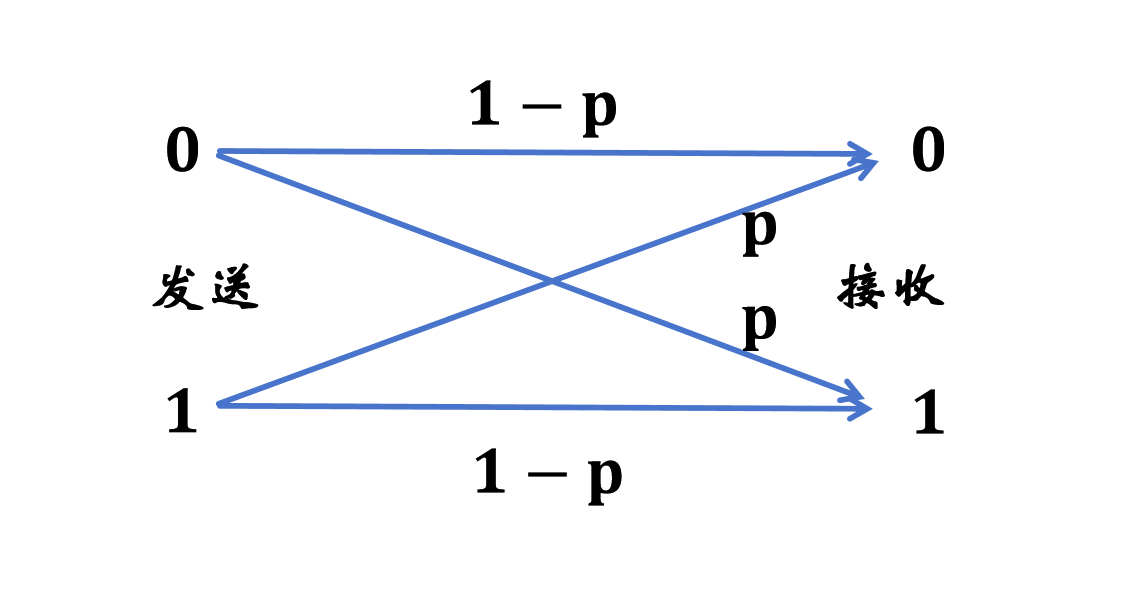
\includegraphics[width=.6\linewidth]{image/3.png}
    \caption{二元对称信道}
    %\label{fig:enter-label}
\end{figure}

信道转移概率矩阵为
$ \left(\begin{array}{cc} 1-p & p \\ p & 1-p\end{array}\right) $

\textbf{2. 二元擦除信道( $\mathrm{M}$ 信道)(有丢失)}

下图所示的信道称为二元擦除信道,输出*表示输入的丢失或擦除.

\begin{figure}[h]
    \centering
    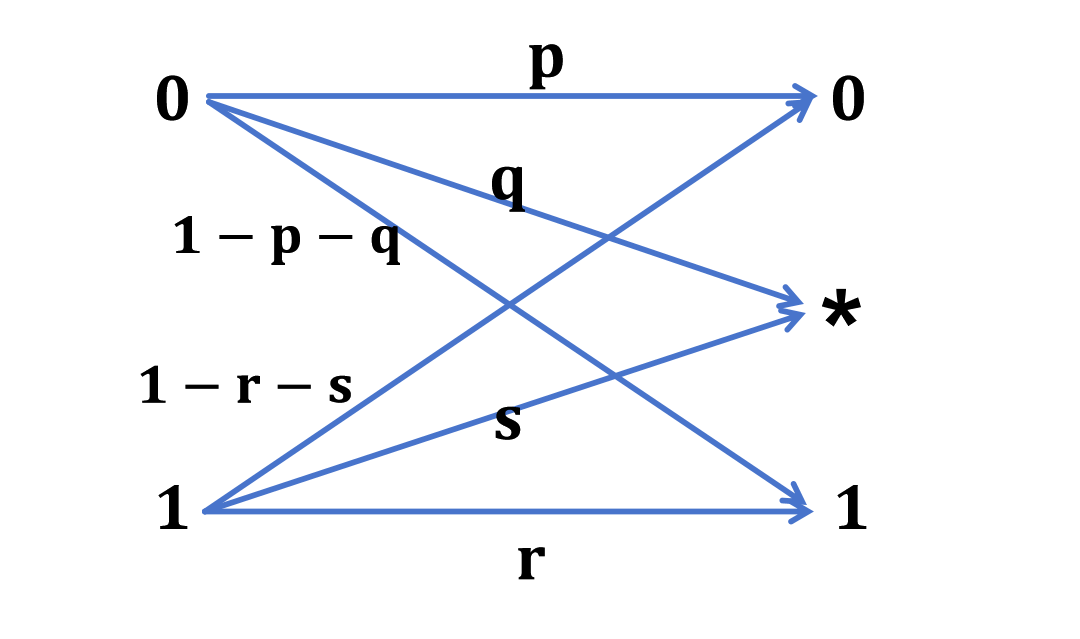
\includegraphics[width=0.5\linewidth]{image/4.png}
    \caption{二元擦除信道}
    %\label{fig:enter-label}
\end{figure}

二元擦除信道的一个特例如下图所示, 称之为 $ M $ 信道, 这个名字来源于它的图类似于字母 $ M $.
$$
p(0 \mid 0)=p(1 \mid 1)=1-p, p(* \mid 0)=p(* \mid 1)=p
$$
\begin{figure}[h]
    \centering
    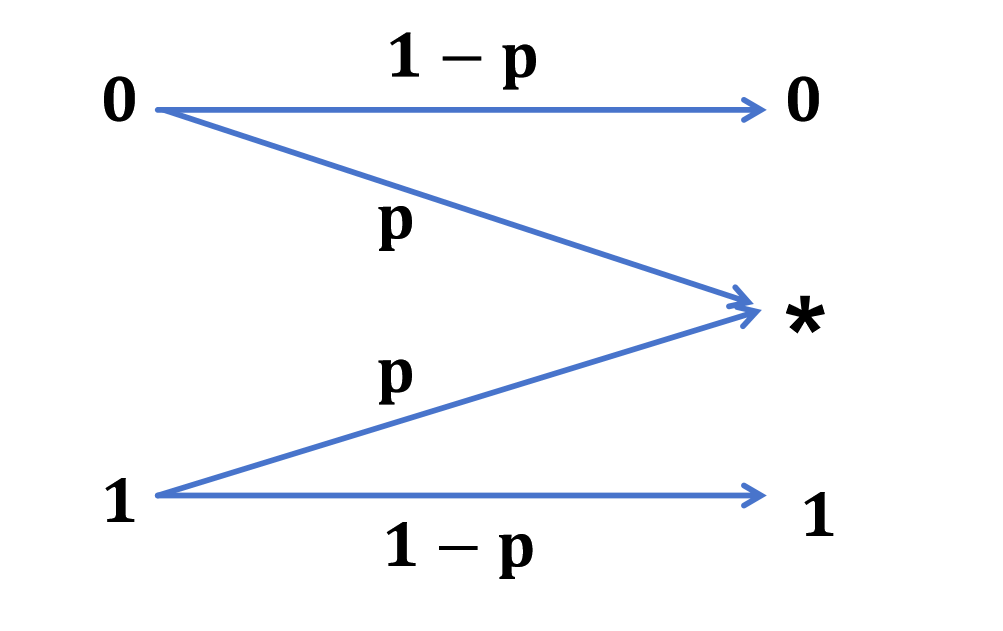
\includegraphics[width=0.5\linewidth]{image/5.png}
    \caption{$M$信道}
    %\label{fig:enter-label}
\end{figure}

\textbf{3. 信道转移概率矩阵} \textbf{(信道矩阵)}

设 $ \mathscr{U}=\left\{u_{1}, u_{2}, \cdots, u_{a}\right\}, \mathscr{V}=\left\{v_{1}, v_{2}, \cdots, v_{b}\right\} $, 定义信道矩阵为
$$
\left(\begin{array}{cccc}
p\left(v_{1} \mid u_{1}\right) & p\left(v_{2} \mid u_{1}\right) & \cdots & p\left(v_{b} \mid u_{1}\right) \\
p\left(v_{1} \mid u_{2}\right) & p\left(v_{2} \mid u_{2}\right) & \cdots & p\left(v_{b} \mid u_{2}\right) \\
\vdots & \vdots & & \vdots \\
p\left(v_{1} \mid u_{a}\right) & p\left(v_{2} \mid u_{a}\right) & \cdots & p\left(v_{b} \mid u_{a}\right)
\end{array}\right)
$$
是一个 $ a \times b $ 阶矩阵, 则该矩阵的每一行对应一个输入字母, 每一列对应一个输出字母,该矩阵的每一行元素之和为 1 , 即
$$
\sum_{j=1}^{b} p\left(v_{j} \mid u_{i}\right)=1, \quad i=1, \cdots, a
$$

按照信道矩阵, 可定义下面几种典型的离散无记忆信道.
\begin{figure}[h]
    \centering
    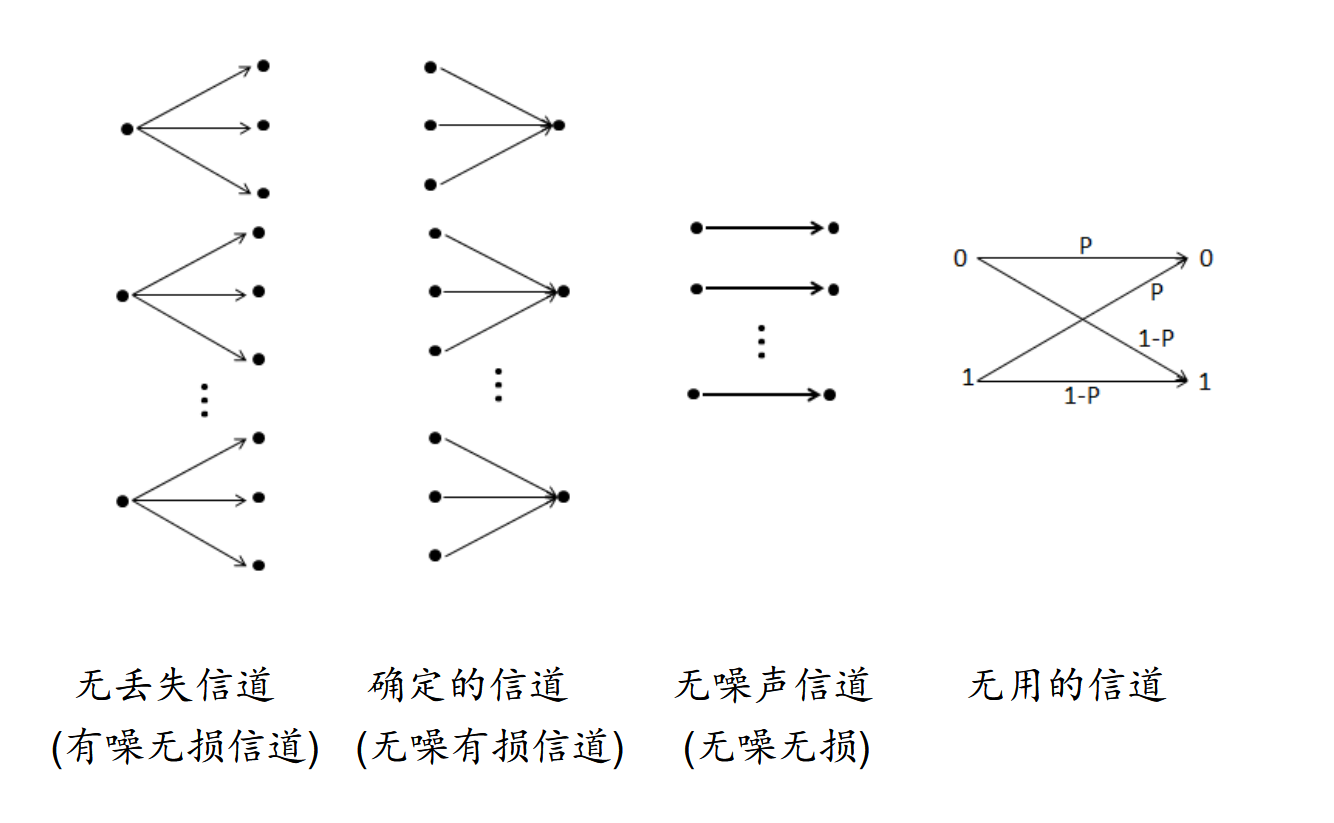
\includegraphics[width=.6\linewidth]{image/6.png}
\end{figure}

\begin{definition}
    (1) 如果输入 $ \xi $ 完全由输出 $ \eta $ 所决定, 称该信道是无丢失的.
    
(2) 如果输出 $ \eta $ 完全由输入 $ \xi $ 所决定,称该信道为决定的(确定的).

(3) 如果信道既是无丢失的也是决定的,称信道是无噪声的.

(4) 如果输入随机变量 $ \xi $ 的知识不能告诉我们任何关于输出 $ \eta $ 的知识,称其为无用的信道.
\end{definition}

\begin{definition}
    根据信道矩阵, 可以定义几种不同信道\\
(1) 如果信道矩阵的每一行是另一行的置换, 则称这个信道是行对称的.\\
(2) 如果信道矩阵的每一列是另一列的置换, 则称这个信道是列对称的.\\
(3) 如果信道矩阵是行对称的, 也是列对称的, 则称这个信道是对称的.
\end{definition}
 
\begin{example}
    具有信道矩阵 $ \left(\begin{array}{cccc}\frac{1}{3} & \frac{1}{3} & \frac{1}{6} & \frac{1}{6} \\ \frac{1}{6} & \frac{1}{6} & \frac{1}{3} & \frac{1}{3}\end{array}\right) $ 和 $ \left(\begin{array}{ccc}\frac{1}{2} & \frac{1}{3} & \frac{1}{6} \\ \frac{1}{6} & \frac{1}{2} & \frac{1}{3} \\ \frac{1}{3} & \frac{1}{6} & \frac{1}{2}\end{array}\right) $ 的信道都是对称的.

信道矩阵为 $ \left(\begin{array}{cccc}\frac{1}{3} & \frac{1}{3} & \frac{1}{6} & \frac{1}{6} \\ \frac{1}{6} & \frac{1}{3} & \frac{1}{6} & \frac{1}{3}\end{array}\right) $ 的信道是行对称的, 但不是列对称信道.
\end{example}

\textbf{4. 行对称信道和列对称信道的主要特征}

\begin{theorem}
     对于行对称信道, 知道 $ \xi $ 时 $ \eta $ 的不确定性与 $ \xi $ 分布无关, 即 $ H(\eta \mid \xi) $ 与入口分布无关.事实上,对任意 $ i=1,2, \cdots, a $, 我们有
$$
H(\eta \mid \xi)=\sum_{j=1}^{b} p\left(v_{j} \mid u_{i}\right) \log \frac{1}{p\left(v_{j} \mid u_{i}\right)}
$$
换句话说,一个信道是行对称的,如果给定输入 $ \xi $ 时关于输出 $ \eta $ 的知识并不依赖于所使用的入口分布.
\end{theorem}
\begin{proof}
    
\end{proof}
 $$ \begin{aligned}H(\eta \mid \xi)&=\sum_{i=1}^{a} p\left(u_{i}\right) H\left(\eta \mid \xi=u_{i}\right) 
=\sum_{i=1}^{a} p\left(u_{i}\right)\left(\sum_{j=1}^{b} p\left(v_{j} \mid u_{i}\right) \log \frac{1}{p\left(v_{j} \mid u_{i}\right)}\right)\\
&=p\left(u_{1}\right) \cdot \sum_{j=1}^{b}\left(p\left(v_{j} \mid u_{1}\right) \log \frac{1}{p\left(v_{j} \mid u_{1}\right)}\right)+p\left(u_{2}\right) \cdot \sum_{j=1}^{b}\left(p\left(v_{j} \mid u_{2}\right) \log \frac{1}{p\left(v_{j} \mid u_{2}\right)}\right) \\
&+\cdots+p\left(u_{a}\right) \cdot \sum_{j=1}^{b}\left(p\left(v_{j} \mid u_{a}\right) \log \frac{1}{p\left(v_{j} \mid u_{a}\right)}\right)
\end{aligned}
$$

因行对称,每行元素互为置换,故
$$
\sum_{j=1}^{b}\left(p\left(v_{j} \mid u_{k}\right) \log \frac{1}{p\left(v_{j} \mid u_{k}\right)}\right)=\sum_{j=1}^{b}\left(p\left(v_{j} \mid u_{\ell}\right) \log \frac{1}{p\left(v_{j} \mid u_{\ell}\right)}\right)
$$

因此有
$$
H(\eta \mid \xi)=\left[p\left(u_{1}\right)+\cdots+p\left(u_{a}\right)\right] \sum_{j=1}^{b} p\left(v_{j} \mid u_{i}\right) \log \frac{1}{p\left(v_{j} \mid u_{i}\right)}, 
\forall i=1,2, \cdots, a .
$$
可得
$$
H(\eta \mid \xi)=\sum_{j=1}^{b} p\left(v_{j} \mid u_{i}\right) \log \frac{1}{p\left(v_{j} \mid u_{i}\right)}
$$
\begin{theorem}
    对于列对称信道,一个均匀入口分布产生一个均匀出口分布.
\end{theorem}
\begin{proof}
设 转移概率矩阵 $ P: $ 一个 $ a \times b $ 矩阵,其中 $ a $ 是输入符号的数量, $ b $ 是输出符号的数量. $ P_{i j} $ 表示从输入 $ i $ 到输出 $ j $ 的概率. 均匀入口分布: 所有输入符号发生的概率相等,即每个输入符号的概率为 $ \frac{1}{a} $ . 为了证明在均匀入口分布下,输出分布也是均匀的,即证明每个输出符号的概率为 $ \frac{1}{b} $ .

对于列对称信道,考虑输出符号 $ j $ 的概率.由全概率公式,输出 $ j $ 的概率 $ P\left(\eta=v_{j}\right) $ 可以表示为:
$$
P\left(\eta=v_{j}\right)=\sum_{i=1}^{a} P\left(\xi=u_{i}\right) P\left(\eta=v_{j} \mid \xi=u_{i}\right)
$$
其中, $ P\left(\xi=u_{i}\right)=\frac{1}{a} $ (因为入口分布是均匀的).
由于信道是列对称的,对于任何固定的 $ j $ ,所有 $ P\left(\eta=v_{j} \mid \xi=u_{i}\right) $都相等,因为每列的概率分布是通过相同的方式置换得到的.设这个常数为 $ c_{j} $ ,那么有:
$$
P\left(\eta=v_{j}\right)=\sum_{i=1}^{a} \frac{1}{a} c_{j}=c_{j}
$$
因为 $ \sum\limits_{i=1}^{a} \frac{1}{a}=1 $ .
要使输出分布均匀,我们需要证明对于所有的 $ j, P\left(\eta=v_{j}\right) $都是相等的.由于列对称性,所有 $ c_{j} $ 实际上都相等,因为每一列都可以通过相同的置换得到其他列,所以它们对应的条件概率相等.由于有 $ b $ 个输出符号,而且它们的概率之和必须为 1 ,所以每个输出符号的概率必须是 $ \frac{1}{b} $ .即,对于所有的 $ j $ ,有 $ P\left(\eta=v_{j}\right)=\frac{1}{b} $ .
\end{proof}



\section{无记忆信道的信道容量}
\subsection*{信道容量的概念}

设 $ \mathscr{C}=(\mathscr{U}, p(v \mid u), \mathscr{V}) $ 是已给信道, 当信道入口分布 $ p(u) $ 给定时, 信道的入口与出口联合分布 $ p(u, v)=p(u) p(v \mid u) $ 确定. 因此, 相应的入口与出口随机变量 $ (\xi, \eta) $ 也就确定. 因此它们的互信息由入口分布 $ p(u) $ 与转移概率 $ p(v \mid u) $ 决定, 因此互信息可写成
$$
I(\xi ; \eta)=I(p(u) ; p(v \mid u)) .
$$

因此当信道 $ \mathscr{C} $ 给定时(也就是信道转移概率 $ p(u \mid v) $ 确定), 互信息就是入口分布 $ p(u) $ 的函数. 以下记
$$
\mathscr{P}_{\mathscr{U}}=\left\{\overline{p} \mid p(u) \geq 0, \sum_{u \in \mathscr{U}} p(u)=1\right\}
$$
为入口分布全体.

\subsection{信道容量的一般定义}

\begin{definition}
    设 $ \mathscr{C} $ 是一个固定信道, 那么定义它的信道容量为互信息 $ I(\xi ; \eta) $ 的最大值,对所有的入口分布 $ \mathscr{P}_{\mathscr{U}} $ 中. 即
$$
C=\max \left\{I=(p(u) ; p(v \mid u)) \mid p(u) \in \mathscr{P}_{\mathscr{U}}\right\} .
$$
如果入口分布 $ p_{0}(u) \in \mathscr{P}_{\mathscr{U}} $, 使 $ I\left(p_{0}(u) ; p(u \mid v)\right)=C $ 成立. 那么称 $ p_{0}(u) $ 为互信息的最大的入口分布,简称为最大入口分布.
\end{definition}

\begin{remark}

    (1)在本章4.2节中,我们已给出了信道序列的最大可达速率的定义. 它与容量在一定条件下可能相等, 但是它们的最初定义的含义是不同的.
    
(2)对记号 $ C $, 我们已给出了三种定义, 即:码元集 $ C $, 信道 $ \mathscr{C} $ 与信道容量$C$. 注意它们的区别.

(3)对 $ \mathscr{P}_{\mathscr{U}} $ 中的元, 我们分别用 $ \overline{p}, p(u), \xi $来表示, 它们都是 $ \mathscr{P}_{\mathscr{U}} $ 中的概率分布或相应的随机变量.
\end{remark}
\begin{example}
 对于二元对称信道,计算它的信道容量.
 
 解: 对于二元对称信道, 它的交叉概率为 $ p $.
$$
\begin{aligned}
I(\xi ; \eta) & =H(\eta)-H(\eta \mid \xi) \\
& =H(\eta)-\sum_{u \in \mathscr{U}} p(u) H(\eta \mid \xi=u) \\
& =H(\eta)-\sum_{u \in \mathscr{U}} p(u) H(p) \\
& =H(\eta)-\left(\sum_{u \in \mathscr{U}} p(u)\right) H(p) \\
& =H(\eta)-H(p) \\
& \leq 1-H(p)
\end{aligned}
$$
注意
$$
\begin{aligned}
H(\eta \mid \xi=0)&=p(0 \mid 0) \log \frac{1}{p(0 \mid 0)}+p(1 \mid 0) \log \frac{1}{p(1 \mid 0)} \\
&=(1-p) \log \frac{1}{1-p}+p \log \frac{1}{p}=H(p), \\
H(\eta \mid \xi=1)&=p(0 \mid 1) \log \frac{1}{p(0 \mid 1)}+p(1 \mid 1) \log \frac{1}{p(1 \mid 1)} \\
&=p \log \frac{1}{p}+(1-p) \log \frac{1}{1-p}=H(p) .
\end{aligned}
$$
如果我们取输入分布为等概分布: $ p_{0}(0)=p_{0}(1)=\frac{1}{2} $, 那么输出分布为 $ q_{0}(0)=q_{0}(1)=\frac{1}{2} $, 这时相应的输入、输出随机变量为 $ \left(\xi_{0}, \eta_{0}\right) $,
$$
I\left(\xi_{0}, \eta_{0}\right)=1-H(p) \geq H(\eta)-H(p)=I(\xi ; \eta)
$$
因此二元对称信道的信道容量为
$$
C=1-H(p)
$$
它的最优入口分布为等概分布.
\end{example}

\begin{example}
 对于 $ M $ 信道, 求它的信道容量.
 
解:$$C=\max \left\{I(\xi ; \eta) \mid \xi \in \mathscr{P}_{\mathscr{U}}\right\}=\max \left\{H(\eta)-H(\eta \mid \xi) \mid \xi \in \mathscr{P}_{\mathscr{U}}\right\}$$
$$
\begin{aligned}
H(\eta \mid \xi=0)&=p(0 \mid 0) \log \frac{1}{p(0 \mid 0)}+p(* \mid 0) \log \frac{1}{p(* \mid 0)}+p(1 \mid 0) \log \frac{1}{p(1 \mid 0)} \\
&=(1-p) \log \frac{1}{1-p}+p \log \frac{1}{p}=H(p) \\
H(\eta \mid \xi=1)&=p(0 \mid 1) \log \frac{1}{p(0 \mid 1)}+p(* \mid 1) \log \frac{1}{p(* \mid 1)}+p(1 \mid 1) \log \frac{1}{p(1 \mid 1)} \\
&=p \log \frac{1}{p}+(1-p) \log \frac{1}{1-p}=H(p) .
\end{aligned}
$$
因此
$$
H(\eta \mid \xi)=\sum_{u \in \mathscr{U}} p(u) H(\eta \mid \xi=u)=\left(\sum_{u \in \mathscr{U}} p(u)\right) H(p)=H(p) $$

$$C=\max \left\{H(\eta)-H(p) \mid \xi \in \mathscr{P}_{\mathscr{U}}\right\} .
$$
现在计算 $ H(\eta) $ 的值, 如取 $ p(0)=\theta, 0 \leq \theta \leq 1 $, 那么我们得到
$$
\begin{aligned}
(q(0), q(*), q(1)) & =(p(0), p(1))\left(\begin{array}{ccc}
1-p & p & 0 \\
0 & p & 1-p
\end{array}\right) \\
& =(\theta, 1-\theta)\left(\begin{array}{ccc}
1-p & p & 0 \\
0 & p & 1-p
\end{array}\right) \\
& =(\theta(1-p), p,(1-\theta)(1-p)) .
\end{aligned}
$$
代入熵的定义计算可得
$$
H(\eta)=(1-p) H(\theta)+H(p) .
$$
因为 $ p $ 是固定常数, 所以 $ H(\eta) $ 的最大值是当 $ \theta=\frac{1}{2} $ 时取得
$$
H\left(\eta_{0}\right)=(1-p) H(\theta)+H(p)=1-p+H(p) .
$$
这时
$$
C=H\left(\eta_{0}\right)-H(p)=1-p .
$$
且当 $ \theta=\frac{1}{2} $ 时达到最大值, 它的最优入口分布为等概率分布.
\end{example}


对于前面定义的几种信道, 可计算它们的信道容量.
\begin{theorem}
(1) 无丢失信道的容量是 $ \log a $, 其中 $ a $ 是输入字母表的大小.

(2) 决定信道的容量是 $ \log b $, 其中 $ b $ 是集合
$ \left\{v_{j} \mid\right. $ 存在某个 $ u_{j} $, 使得 $ q\left(v_{j} \mid u_{i}\right)=1 $ 成立 $ \} $
的元素个数.

(3) 无噪声信道的容量是 $ \log a $, 其中 $ a $ 是输入字母表的大小.

(4) 无用信道的容量是0.
\end{theorem}
\begin{proof}
(1) 因  $\xi$  完全由  $\eta$决定,即 $ H(\xi \mid \eta)=0 $.
$$
\begin{aligned}
I(\xi ; \eta)  =H(\xi)-H(\xi \mid \eta)  =H(\xi)-0  =H(\xi) \leq \log a
\end{aligned}
$$
$ H(\xi) $ 的最大值 $ \log a $.

(2) $ I(\xi ; \eta)=H(\eta)-H(\eta \mid \xi)=H(\eta) \leq \log b $.

(3) 无噪声信道等价条件是, 存在一个 $ \mathscr{U} \rightarrow \mathscr{V} $ 的 $ 1-1 $ 映射 $ \phi $, 使得 $ p(\phi(u) \mid u)=1 $ 对所有 $ u $ 成立, 从而 $ a=b $. 因此 $ C=\log a=\log b $.

(4) 无用信道意味着输出不依赖于输入,或者说输出对于输入的选择完全没有信息.在这种情况下,无论输入是什么,输出的分布都保持不变,因此 \(H(\eta | \xi) = H(\eta)\). $ I(\xi ; \eta)=H(\xi)-H(\xi \mid \eta)=H(\xi)-H(\xi)=0 $. (注意 $ \xi $ 与 $ \eta $ 是相互独立的.)
\end{proof}

下面计算对称信道的信道容量.
\begin{theorem}
 对称信道的信道容量为
$$
C=\log b-\sum_{j=1}^{b} p\left(v_{j} \mid u_{i}\right) \log \frac{1}{p\left(v_{j} \mid u_{i}\right)}
$$
对 $ \forall i=1,2, \cdots, a $ 都成立,而且它的最大入口分布为均匀分布 $ p\left(u_{i}\right)=\frac{1}{a} $
\end{theorem}
\begin{proof}
    $$
I(\xi ; \eta)=H(\eta)-H(\eta \mid \xi) \leq \log b-H(\eta \mid \xi),
$$
其中
$$
H(\eta \mid \xi)=\sum_{i=1}^{a} p\left(u_{i}\right)\left(\sum_{j=1}^{b} p\left(v_{j} \mid u_{i}\right) \log \frac{1}{p\left(v_{j} \mid u_{i}\right)}\right)
$$
因为信道的对称性,括号里面的和与 $ i $ 无关,所以
$$
\begin{aligned}
H(\eta \mid \xi) & =\left(\sum_{j=1}^{b} p\left(v_{j} \mid u_{i}\right) \log \frac{1}{p\left(v_{j} \mid u_{i}\right)}\right)\left(\sum_{i=1}^{a} p\left(u_{i}\right)\right) \\
& =\sum_{j=1}^{b} p\left(v_{j} \mid u_{i}\right) \log \frac{1}{p\left(v_{j} \mid u_{i}\right)} .
\end{aligned}
$$
可见 $ H(\eta \mid \xi) $ 与 $ \xi $ 的分布无关. 因此当我们取入口分布为均匀分布 $ p(u)=\frac{1}{a} $ 时, 相应的出口分布为
$$
q(v)=\sum_{u \in \mathscr{U}} p(u) p(v \mid u)=\frac{1}{a} \sum_{u \in \mathscr{U}} p(v \mid u) .
$$
由对称信道的定义可知, $ \sum\limits_{u \in \mathscr{U}} p(v \mid u) $ 与 $ v $ 无关, 因此 $ q(v) $ 与 $ v $ 无关,是个均匀分布. 这时 $ \log b $ 是 $ H(\eta) $ 的最大值. 于是,
$$
C=\log b-H(\eta \mid \xi)=\log b-\sum_{j=1}^{b} p\left(v_{j} \mid u_{i}\right) \log \frac{1}{p\left(v_{j} \mid u_{i}\right)}
$$
为对称信道的信道容量, 它的最大入口分布为均匀分布.
\end{proof}

\begin{example}
 对于二元对称信道, 转移矩阵为 $ \left(\begin{array}{cc}1-p & p \\ p & 1-p\end{array}\right) $.
于是 $$ C=\log 2-(1-p) \log \frac{1}{1-p}-p \log \frac{1}{p} =1-H(p) $$
\end{example}
\begin{example}
    信道的转移概率矩阵为 $ P=\left(\begin{array}{cccc}\frac{1}{3} & \frac{1}{3} & \frac{1}{6} & \frac{1}{6} \\ \frac{1}{6} & \frac{1}{6} & \frac{1}{3} & \frac{1}{3}\end{array}\right) $, 求其信道容量. $ |\mathscr{U}|=2,|\mathscr{V}|=4 $

解:该信道为对称信道,故
$$
\begin{aligned}
C= & \log b-\sum_{j=1}^{b} p\left(v_{j} \mid u_{i}\right) \log \frac{1}{p\left(v_{j} \mid u_{i}\right)}  =\log 4-\sum_{j=1}^{4} p\left(v_{j} \mid u_{i}\right) \log \frac{1}{p\left(v_{j} \mid u_{i}\right)} \\
& =2-2 \times \frac{1}{3} \log 3-2 \times \frac{1}{6} \log 6  =2-\frac{2}{3} \log 3-\frac{1}{3} \log 6 \\
& =2-\frac{2}{3} \log 3-\frac{1}{3} \log 3-\frac{1}{3}  =2-\log 3-\frac{1}{3}  \approx 0.082 \text { 比特/符号. }
\end{aligned}
$$
\end{example}

\subsection{无记忆信道序列的容量性质}
设 $ \mathscr{C}^{n} $ 是离散无记忆信道序列,同样可以定义 $ \mathscr{U}^{n} $ 上的全体概率分布 $ \mathscr{P}_{\mathscr{U}^{n}} $, 那么对 $ p^{(n)}\left(u^{(n)}\right) $, 可以确定联合分布
$$
p^{(n)}\left(u^{(n)}, v^{(n)}\right)=p^{(n)}\left(u^{(n)}\right) p\left(v^{(n)} \mid u^{(n)}\right)=p^{(n)}\left(u^{(n)}\right) \prod_{j=1}^{n} p\left(v_{j} \mid u_{j}\right)
$$
及相应的入口与出口随机变量 $ \left(\xi^{(n)}, \eta^{(n)}\right) $, 于是可定义它们的互信息
$$
\begin{aligned}
I\left(\xi^{(n)} ; \eta^{(n)}\right)&=I\left(p^{(n)}\left(u^{(n)}\right) ; p^{(n)}\left(v^{(n)} \mid u^{(n)}\right)\right) \\
&=\sum_{\left(u^{(n)} \times v^{(n)}\right) \in \mathscr{U}^{n} \times \mathscr{V}^{n}} p^{(n)}\left(u^{(n)}, v^{(n)}\right) \log \left(\frac{p^{(n)}\left(u^{(n)}, v^{(n)}\right)}{p^{(n)}\left(u^{(n)}\right) q^{(n)}\left(v^{(n)}\right)}\right)
\end{aligned}
$$
其中 $q^{(n)}\left(u^{(n)}\right)=\sum\limits_{u^{(n)} \in \mathscr{U}^{n}} p^{(n)}\left(u^{(n)}\right) p^{(n)}\left(v^{(n)} \mid u^{(n)}\right) $


\begin{definition}
    信道序列 $ \mathscr{C}_{n} $ 的信道容量定义为
$$
C_{n}=\max \left\{I\left(p^{(n)}\left(u^{(n)}\right) ; p^{(n)}\left(v^{(n)} \mid u^{(n)}\right)\right) \mid p^{(n)}\left(u^{(n)}\right) \in \mathscr{P}_{\mathscr{U}^{n}}\right\}
$$
\end{definition}

无记忆信道序列容量的性质
\begin{definition}
    设 $ \mathscr{Z} n $ 是任一有限集合 $ \mathscr{Z} $ 上的 $ n $ 维乘积空间, $ p(z) $ 是 $ \mathscr{Z} $ 上的一个概率分布. 如果 $ p^{(n)}\left(z^{(n)}\right)=\prod\limits_{i=1}^{n} p\left(z_{i}\right) $, 则称概率分布 $ p^{(n)}\left(z^{(n)}\right) $ 为由 $ p(z) $ 确定的无记忆概率分布.
\end{definition}

\begin{theorem}
    如果 $ \mathscr{C}^{n} $ 是由 $ \mathscr{C} $ 确定的无记忆信道,它们的信道容量分别为 $ C_{n} $ 与 $ C $, 那么必有 $ C_{n}=n C $ 成立, 且 $ \mathscr{C}^{n} $ 的最大入口分布为 $ p_{0}^{(n)}\left(u^{(n)}\right) $ 是 $ p_{0}(u) $ 确定的无记忆分布, 其中 $ p_{0}(u) $ 是信道 $ \mathscr{C} $ 的最大入口分布.
\end{theorem}


















\section{信道容量的计算}

在4.3节我们给出了信道容量的定义并求出了一些特殊信道的容量,但对于一般的信道,求它的容量并不是件容易的事.在这一节中我们给出一些计算信道容量的方法.

\subsection{凸函数的极大值性质}

因为信道容量是互信息的最大值, 所以为了求得某个信道的容量, 先研究这个信道的输入和输出之间的互信息.如前所记, 信道的输入和输出字母表分别是
$$
\mathscr{U}=\left\{u_{1}, u_{2}, \cdots, u_{a}\right\} \quad \mathscr{V}=\left\{v_{1}, v_{2}, \cdots, v_{b}\right\},
$$
信道的转移概率矩阵 $ p\left(v_{j} \mid u_{i}\right) $ 给定. 因此信道容量的计算问题就是求
$$
I(\xi ; \eta)=I(p(u) ; p(v \mid u)) \quad p(u) \in \mathscr{P}_{\mathscr{U}}
$$
的最大值问题.

记入口分布 $ \overline{p}=\left\{p\left(u_{1}\right), p\left(u_{2}\right), \cdots, p\left(u_{a}\right)\right\} $,我们可以把互信息写成如下形式:
$$
I(\xi ; \eta)=\sum_{i=1}^{a} \sum_{j=1}^{b} p\left(u_{i}\right) p\left(v_{j} \mid u_{i}\right) \log \frac{p\left(v_{j} \mid u_{i}\right)}{\sum\limits_{\ell=1}^{a} p\left(u_{\ell}\right) p\left(v_{j} \mid u_{\ell}\right)} .
$$

\begin{lemma}
    对固定的转移概率 $ p(v \mid u) $, 互信息
$$
I(\overline{p})=I(p(u) ; p(v \mid u))
$$
是 $ \overline{p} $ 上的凸函数.
\end{lemma}
\begin{lemma}
    设 $ f(\overline{p}) $ 是有 $ n $ 个输入变量的连续上凸函数, 输入 $  \overline{p}=\left(p_{1}, p_{2}, \cdots, p_{a}\right) $ 满足
$$
\sum_{i=1}^{a} p_{i}=1, \quad p_{i} \geq 0, \quad i=1,2, \cdots, a
$$
且函数的偏导数 $ \partial f(\overline{p}) / \partial p_{i}, i=1,2, \cdots, a $ 有定义且连续, 则函数 $ f(\overline{p}) $ 对于 $ \overline{p}^{*}=\left(p_{1}^{*}, \cdots, p_{a}^{*}\right) $ 取最大值的充要条件为存在某一实数 $ \lambda $, 且满足
$$
\begin{array}{ll}
\dfrac{\partial f\left(\overline{p}^{*}\right)}{\partial p_{i}^{*}}=\lambda, & \text { 对 } p_{i}^{*}>0 \text { 的 } i, \\
\dfrac{\partial f\left(\overline{p}^{*}\right)}{\partial p_{i}^{*}} \leq \lambda, & \text { 对 } p_{i}^{*}=0 \text { 的 } i .
\end{array}
$$
\end{lemma}
\begin{remark}

(1)只需证明对于其他输入 $ \overline{p} $, 都有 $ f(\overline{p}) \leq f\left(\overline{p}^{*}\right) $
    
(2) 求函数极值的方法: 对 $ p_{i}^{*}>0 $ 的 $ i,\left.\dfrac{\partial f(\overline{p})}{\partial p_{i}}\right|_{\overline{p}=p^{*}}=\lambda $ 时, $ f(\overline{p}) $ 取得最大值.
\end{remark}


\subsection{信道容量的计算}
我们下面只讲用极值法求信道容量的方法, 利用迭代法求信道容量的方法不讲.

\begin{theorem}
    一个信道的入口分布 $ \overline{p}^{*}=\left(p^{*}\left(u_{1}\right), \cdots, p^{*}\left(u_{s}\right)\right) $ 使得输入和输出之间的互信息达到最大值的充要条件是存在一个常数 $ C $, 满足
$$
\begin{aligned}
\sum_{j=1}^{b} p\left(v_{j} \mid u_{i}\right) \log \frac{p\left(v_{j} \mid u_{i}\right)}{\sum\limits_{\ell=1}^{a} p^{*}\left(u_{\ell}\right) p\left(v_{j} \mid u_{\ell}\right)}&=C, \quad \text { 对于 } p^{*}\left(u_{i}\right)>0, \\
\sum_{j=1}^{b} p\left(v_{j} \mid u_{i}\right) \log \frac{p\left(v_{j} \mid u_{i}\right)}{\sum\limits_{\ell=1}^{a} p^{*}\left(u_{\ell}\right) p\left(v_{j} \mid u_{\ell}\right)} &\leq C, \quad \text { 对于 } p^{*}\left(u_{i}\right)=0 .
\end{aligned}
$$
这时 $ C $ 即为信道容量.
\end{theorem}
\begin{proof}
 令 $ I(\xi ; \eta)=I(p) $. 由引理 , 互信息达到信道容量的充要条件为存在一常数 $ \lambda $, 使得:
$$
\begin{aligned}
\left.\frac{\partial I(\overline{p})}{\partial p_{i}}\right|_{\overline{p}=p^{*}}=\lambda, \quad p_{i}^{*}>0, \\
\left.\frac{\partial I(\overline{p})}{\partial p_{i}}\right|_{\overline{p}=p^{*}} \leq \lambda, \quad p_{i}^{*}=0 . 
\end{aligned}
$$

$$I(\overline{p})=\sum_{i=1}^{a} \sum_{j=1}^{b} p\left(u_{i}\right) p\left(v_{j} \mid u_{i}\right) \log p\left(v_{j} \mid u_{i}\right)- 
\sum_{i=1}^{a} \sum_{j=1}^{b} p\left(u_{i}\right) p\left(v_{j} \mid u_{i}\right) \log \left(\sum_{\ell=1}^{a} p\left(u_{\ell}\right) p\left(v_{j} \mid u_{\ell}\right)\right)$$

对 $ p_{i}\left(p\left(u_{i}\right)\right) $ 求偏导,则其它的 $ p\left(u_{j}\right) $ 视为常数,求偏导为 0 .

$$ \begin{aligned} \frac{\partial I(\bar{p})}{\partial p_{i}}&= \sum_{j=1}^{b} p\left(v_{j} \mid u_{i}\right) \log p\left(v_{j} \mid u_{i}\right)-\sum_{j=1}^{b} p\left(v_{j} \mid u_{i}\right) \log \left(\sum_{\ell=1}^{a} p\left(u_{\ell}\right) p\left(v_{j} \mid u_{\ell}\right)\right) \\ &-\sum_{k=1}^{a} \sum_{j=1}^{b} p\left(u_{k}\right) p\left(v_{j} \mid u_{k}\right) \frac{p\left(v_{j} \mid u_{i}\right)}{\sum\limits_{\ell=1}^{a} p\left(u_{\ell}\right) p\left(v_{j} \mid u_{\ell}\right)} \\ &=\sum_{j=1}^{b} p\left(v_{j} \mid u_{i}\right) \log \frac{p\left(v_{j} \mid u_{i}\right)}{q\left(v_{j}\right)}-\sum_{j=1}^{b}\left(\sum_{k=1}^{a} p\left(u_{k}\right) p\left(v_{j} \mid u_{k}\right)\right) \frac{p\left(v_{j} \mid u_{i}\right)}{\sum\limits_{\ell=1}^{a} p\left(u_{\ell}\right) p\left(v_{j} \mid u_{\ell}\right)} \\ &=\sum_{j=1}^{b} p\left(v_{j} \mid u_{i}\right) \log \frac{p\left(v_{j} \mid u_{i}\right)}{q\left(v_{j}\right)}-\sum_{j=1}^{b} p\left(v_{j} \mid u_{i}\right) \frac{\sum\limits_{k=1}^{a} p\left(u_{k}\right) p\left(v_{j} \mid u_{k}\right)}{\sum\limits_{\ell=1}^{a} p\left(u_{\ell}\right) p\left(v_{j} \mid u_{\ell}\right)} \\ &=\sum_{j=1}^{b} p\left(v_{j} \mid u_{i}\right) \log \frac{p\left(v_{j} \mid u_{i}\right)}{q\left(v_{j}\right)}-\sum_{j=1}^{b} p\left(v_{j} \mid u_{i}\right) \\ &=\sum_{j=1}^{b} p\left(v_{j} \mid u_{i}\right) \log \frac{p\left(v_{j} \mid u_{i}\right)}{q\left(v_{j}\right)}-1\\
&=\sum_{j=1}^{b} p\left(v_{j} \mid u_{i}\right) \log \frac{p\left(v_{j} \mid u_{i}\right)}{\sum\limits_{\ell=1}^{a} p\left(u_{\ell}\right) p\left(v_{j} \mid u_{\ell}\right)}-1
\end{aligned} $$
令
$$
\lambda=\left.\frac{\partial I(\overline{p})}{\partial p_{i}}\right|_{p=p^{*}},
$$
则
$$
\lambda=\sum_{j=1}^{b} p\left(v_{j} \mid u_{i}\right) \log \frac{p\left(v_{j} \mid u_{i}\right)}{\sum\limits_{k=1}^{a} p_{k}^{*} p\left(v_{j} \mid u_{k}\right)}-1
$$
两边同时乘以 $ p_{i}^{*} $ 再对 $ i $ 求和有
$$
\begin{aligned}
\lambda & =\sum_{i=1}^{a} p_{i}^{*} \frac{\partial I(\overline{p})}{\partial p_{i}} \mid_{ p=p^{*}} \\
& =\sum_{i=1}^{a} \sum_{j=1}^{b} p_{i}^{*} p\left(v_{j} \mid u_{i}\right) \log \frac{p\left(v_{j} \mid u_{i}\right)}{\sum\limits_{k=1}^{a} p_{k}^{*} p\left(v_{j} \mid u_{k}\right)}-\sum_{i=1}^{a} p_{i}^{*} \\
& =\sum_{i=1}^{a} \sum_{j=1}^{b} p_{i}^{*} p\left(v_{j} \mid u_{i}\right) \log \frac{p\left(v_{j} \mid u_{i}\right)}{\sum\limits_{k=1}^{a} p_{k}^{*} p\left(v_{j} \mid u_{k}\right)}-1 \\
& =I\left(\bar{p}^{*}\right)-1=C-1
\end{aligned}
$$
根据第二个引理 $, I(\overline{p}) $ 在 $ \overline{p}^{*} $ 取最大值 $ I\left(\bar{p}^{*}\right), C=I\left(p^{*}\right)=\lambda+1 $.
$$
C=\sum_{j=1}^{b} p\left(v_{j} \mid u_{i}\right) \log \frac{p\left(v_{j} \mid u_{i}\right)}{\sum\limits_{\ell=1}^{a} p^{*}\left(u_{\ell}\right) p\left(v_{j} \mid u_{\ell}\right)}, \quad \text { 对于 } p^{*}\left(u_{i}\right)>0 \text {. }
$$
\end{proof}

\begin{example}
对于 $ M $ 信道, 它的信道矩阵为
$$
\left(\begin{array}{ccc}
1-p & 0 & p \\
0 & 1-p & p
\end{array}\right), \quad 0<p<1 .
$$
设入口分布为 $ \overline{p}=\left(p_{0}, p_{1}\right) $, 对应的出口分布为 $ \overline{q}=\left\{q_{0}, q_{1}, q_{2}\right\} $,而 $ q\left(v_{j}\right)=\sum\limits_{i=1}^{a} p\left(u_{i}\right) p\left(v_{j} \mid u_{i}\right) $.
由定理的结论知
$$
\begin{aligned}
C&=\sum_{j=1}^{b} p\left(v_{j} \mid u_{i}\right) \log \frac{p\left(v_{j} \mid u_{i}\right)}{\sum\limits_{\ell=1}^{a} p\left(u_{\ell}\right) p\left(v_{j} \mid u_{\ell}\right)}\\ & =\sum_{j=1}^{b} p\left(v_{j} \mid u_{i}\right) \log \frac{p\left(v_{j} \mid u_{i}\right)}{q\left(v_{j}\right)} \\
& =(1-p) \log \frac{1-p}{q_{0}}+p \log \frac{p}{q_{2}}  =(1-p) \log \frac{1-p}{q_{1}}+p \log \frac{p}{q_{2}}
\end{aligned}
$$
于是有 $ q_{0}=q_{1} $,
而
$$
\begin{aligned}
\left(q_{0}, q_{1}, q_{2}\right)  =\left(p_{0}, p_{1}\right)\left(\begin{array}{ccc}
1-p & 0 & p \\
0 & 1-p & p
\end{array}\right) =\left(p_{0}(1-p), p_{1}(1-p), p\right) .
\end{aligned}
$$
由 $ q_{0}=q_{1} $ 知, $ p_{0}=p_{1} \Rightarrow p_{0}=p_{1}=\frac{1}{2}, \quad q_{0}=q_{1}=\frac{1-p}{2}, q_{2}=p $,于是有 $ C=1-p $.
\end{example}


\section{信道的编码和译码问题}
在本章4.2节中,我们已给出了信道序列的可达速率的定义, 它的实质是存在适当的编码与译码算法, 使消息传递的误差很小, 而且可以转送一定数量的数据量.
我们现在给出一个关于信道序列的可达速率的等价条件. 我们仍记
$$
\mathscr{C}^{n}=\left(\mathscr{U}^{n}, p\left(v^{(n)}\right) \mid u^{(n)}, \mathscr{V}^{n}\right)
$$
为信道序列, 记 $ \mathscr{S}^{n}=\left\{\mathscr{X}^{n}, p^{(n)}\left(x^{n}\right)\right\} $ 为信源序列, 在4.1节中我们已经给出可达速率 $ R $ 的定义, 且取信源序列为 $ \mathscr{S}^{n} $
$$
\left\{\begin{array}{l}
\mathscr{X}^{n}=\mathscr{Y}^{n}=\left\{1,2, \cdots, M_{n}\right\}, \\
P^{(n)}\left(x^{(n)}\right)=\frac{1}{M_{n}}, \text { 对任何 } x^{(n)} \in \mathscr{X}^{n},
\end{array}\right.
$$
所给,那么信道的编码问题就是求信道序列的最大可达速率问题. 为讨论这个问题, 我们先给出 $ R $ 是可达速率的一个等价条件, 由这个等价条件也可看到信道的编码问题的本质.

\begin{definition}
    信道序列仍记为 $ \mathscr{C}^{n} $. 我们称
$$
\left(u_{i}^{(n)}, \mathscr{B}_{i}^{(n)}\right), i=1,2, \cdots, M_{n}
$$
是 $ \mathscr{C}^{n} $ 的一组 $ \epsilon $ 专线,如果它满足以下条件.

(1) $ u_{i}^{(n)} \in \mathscr{U}^{n} $, 它们互不相同.

(2) $ \mathscr{B}_{i}^{(n)} $ 是 $ \mathscr{V}^{n} $ 的一组子集, 它们互不相交, 即
$$
\mathscr{B}_{i}^{(n)} \cap \mathscr{B}_{j}^{(n)}=\emptyset \text {, 当 } i \neq j \text { 时, }
$$

(3)对任何 $ i=1,2, \cdots, M_{n} $, 有 $ P^{(n)}\left(\mathscr{B}_{i}^{(n)} \mid u_{i}^{(n)}\right)>1-\epsilon $ 成立.称式 中的 $ M_{n} $ 为 $ \epsilon $ 专线的数目.
\end{definition}

通过以下定理可以看到, $ \epsilon $ 专线与可达速率的关系问题.
\begin{theorem}
    $ R $ 是信道序列 $ \mathscr{C}^{n} $ 可达速率的充分与必要条件是存在数列 $ \epsilon_{n} \rightarrow 0 $, 使 $ \mathscr{C}^{n} $ 有 $ M_{n}>2^{n R\left(1-\epsilon_{n}\right)} $ 条 $ \epsilon_{n} $ 专线.
\end{theorem}
该定理不证明, 掌握结论.

具有 $ \epsilon_{n} $ 专线的编、译码的信息传输图如图所示.

\begin{figure}[h]
    \centering
    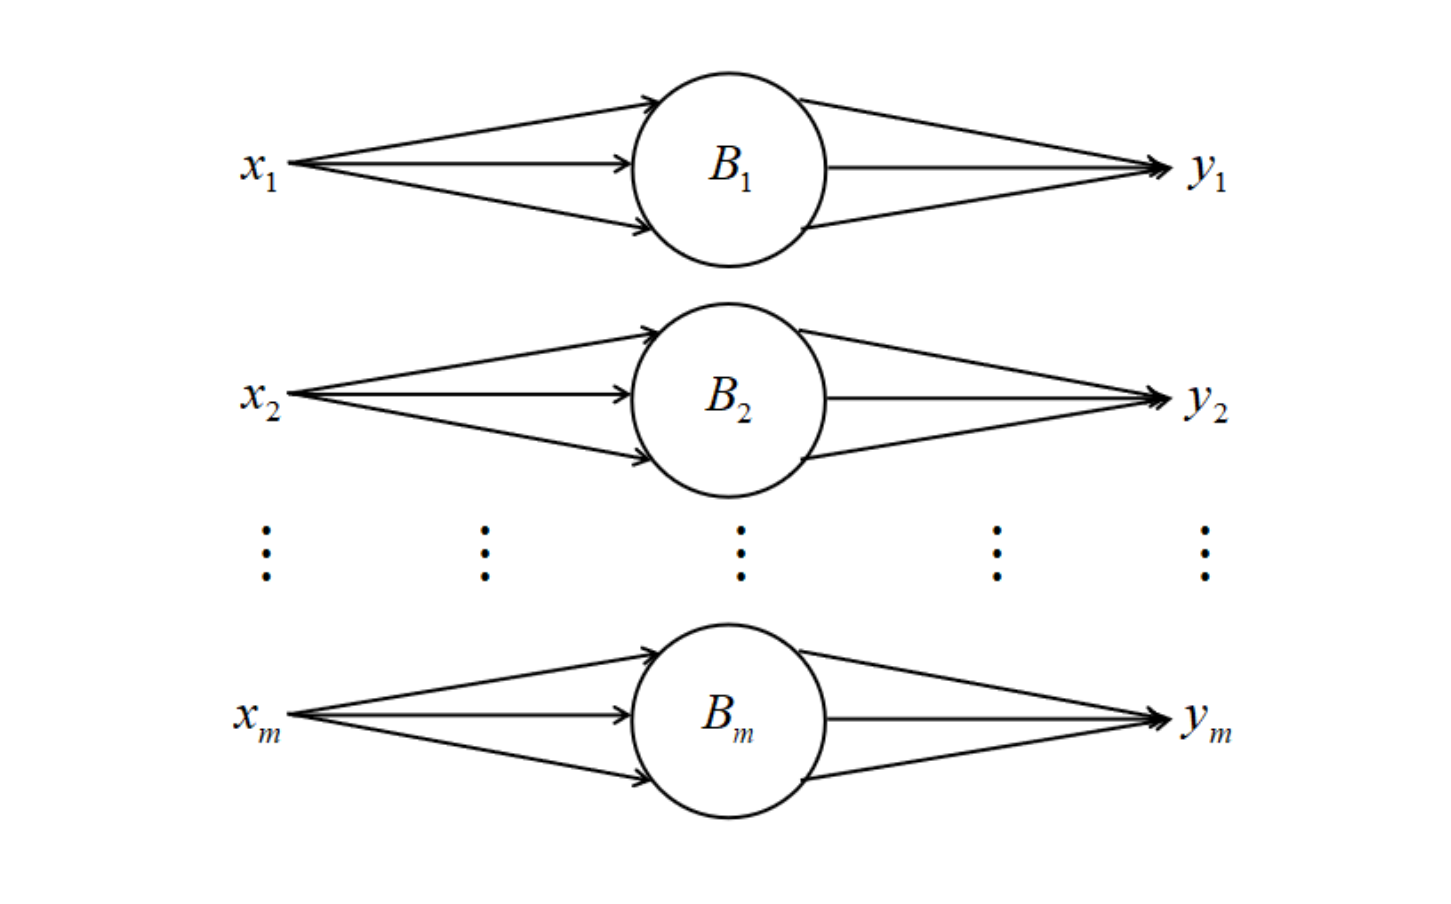
\includegraphics[width=0.5\linewidth]{image/7.png}
    \caption{$ \epsilon $ 专线的编码和译码判决方案表示图}
\end{figure}
可以看出, 专线对通信系统的编码和译码方式给出了一个形象的描述, 对我们理解通信编码问题很有帮助.


\section{信道的正编码定理和反编码定理}
在前几节中, 我们已给出了信道序列的最大可达速率与信道容量的定义.我们现在讨论它们的相互关系问题.这就是信道编码定理.

\begin{theorem}[信道编码的正编码定理]
    如果 $ C $ 是一个离散无记忆信道 $ \mathscr{C} $ 的信道容量, 那么 $ C $ 必是该离散无记忆信道序列的一个可达速率.
\end{theorem}
\begin{proof}
    关于信道编码定理的证明有许多种方法,较为精确的证明方法为组合法, 但它涉及许多排列组合的计算. 另外, 还可以利用 $ \epsilon $ 专线的方法给以证明, 该方法是编码定理的经典证明方法, 很为直观. 在本书中我们采用随机码的方法给以证明, 这是一种很为巧妙的证明方法,在信息论中广为使用. 对此我们分以下几步给出证明思路.

    1. 随机码的定义

因为 $ \mathscr{C}^{n} $ 是离散无记忆信道序列,所以它的转移概率分布为
$$
p^{(n)}\left(v^{(n)} \mid u^{(n)}\right)=\prod_{i=1}^{n} p\left(v_{i} \mid u_{i}\right)
$$
它由 $ \mathscr{C}=\{\mathscr{U}, P(v \mid u), \mathscr{V}\} $ 决定. 记 $ p_{0}(u) $ 是信道的入口分布,使 $ I\left(p_{0}(u) ; p(v \mid u)\right)=C $ 成立. 设 $ \mathscr{S} $ 为具有均匀分布的信源,
\begin{equation}
    \mathscr{X}^{n}=\left\{1,2, \cdots, M_{n}\right\}, P^{(n)}(i)=\frac{1}{M_{n}}
\end{equation}
那么随机码的定义为 $ \mathscr{X}^{n} \rightarrow \mathscr{U}^{n} $ 的一组随机映射
\begin{equation}\label{4.6.2}
\overline{f}^{*}=\left\{f_{1}^{*}, f_{2}^{*}, \cdots, f_{M_{n}}^{*}\right\}
\end{equation}
它满足以下条件.\\
(1) $ M_{n}=\left|\mathscr{X}^{n}\right| $ 是信源字母表的元素个数.\\
(2) $ f_{1}^{*}, f_{2}^{*}, \cdots, f_{M_{n}}^{*} $ 一组独立同分布的随机变量.\\
(3) 每个 $ f^{*} $ 在 $ \mathscr{U}^{n} $ 中取值, 并具有分布为
$$
p_{0}^{(n)}\left(u^{(n)}\right)=\prod_{i=1}^{n} p\left(u_{i}\right)
$$

随机码 $ \overline{f}^{*} $ 的一个样本值记为
\begin{equation}\label{4.6.3}
\overline{f}^{(n)}=\left\{f_{1}^{(n)}, f_{2}^{(n)}, \cdots, f_{M_{n}}^{(n)}\right\}=\left\{u_{1}^{(n)}, u_{2}^{(n)}, \cdots, u_{M_{n}}^{(n)}\right\}
\end{equation}
它就是 $ \mathscr{X}^{n} \rightarrow \mathscr{U}^{n} $ 的一个编码.

如果信道的输入概率分布为 $ p_{0}^{(n)}\left(u^{(n)}\right) $ 与信道转移概率分布 $ p^{(n)}\left(v^{(n)} \mid u^{(n)}\right) $, 那么信道输入与输出的联合概率分布密度与互信息密度函数确定,它们分别为
$$
p_{0}^{(n)}\left(u^{(n)}, v^{(n)}\right)=p_{0}^{(n)}\left(u^{(n)}\right) p^{(n)}\left(v^{(n)} \mid u^{(n)}\right)
$$
及
$$
i_{0}\left(u^{(n)} ; v^{(n)}\right)=\log \left(\frac{p_{0}^{(n)}\left(u^{(n)}, v^{(n)}\right)}{p_{0}^{(n)}\left(u^{(n)}\right) q_{0}^{(n)}\left(v^{(n)}\right)}\right)
$$
由于输入概率分布 $ p_{0}^{(n)}\left(u^{(n)}\right) $ 、信道转移概率分布 $ p^{(n)}\left(v^{(n)} \mid u^{(n)}\right) $是无记忆的, 可知 $ p_{0}^{(n)}\left(u^{(n)}, v^{(n)}\right) $, \\$q_{0}^{(n)}\left(v^{(n)}\right) $ 是无记忆的.

因此互信息密度函数为
\begin{equation}\label{4.6.4}
i_{0}\left(u^{(n)} ; v^{(n)}\right)=\sum_{j=1}^{n} \log \left(\frac{p_{0}\left(u_{j}, v_{j}\right)}{p_{0}\left(u_{j}\right) q_{0}\left(v_{j}\right)}\right)
\end{equation}

2. 阈值译码算法与带随机编码的通信系统

阈值译码算法的定义如下.
\begin{definition}
    如果 $ \overline{f} $ 是由式(\ref{4.6.3})给定的随机编码样本, 那么它的码元集合也由式(\ref{4.6.3})给定. 如果 $ v^{(n)} $ 是信道序列的一个输出向量,那么以下的译码算法为阈值译码算法,
\begin{equation}\label{4.6.5}
    g\left(v^{(n)}\right)=\left\{\begin{array}{ll}
j, & \text { 如果 } i_{0}\left(u_{j}^{(n)} ; v^{n}\right)>K_{n} \\
1, & \text { 否则. }
\end{array}\right.
\end{equation}
其中 $ K_{n} $ 是一个适当的常数, 我们称之为阈值.
\end{definition}


由以上定义, 我们得到一个带有随机编码的通信系统, 并记之为
\begin{equation}\label{4.6.6}
\varepsilon^{*}=\left\{\overline{f}^{*}, \mathscr{C}\right\}=\left\{j, f_{j}^{*}, v_{j}^{*}, g\left(v_{j}^{*}\right): j=1,2, \cdots, M_{n}\right\},
\end{equation}

对此模型, 我们说明如下.\\
(1) 在式(\ref{4.6.6})中, $ j $ 是消息字母,它的取值概率为 $ \operatorname{Pr}\{\tilde{\xi}=j\}=\frac{1}{M_{n}} $.\\
(2) $ f_{j}^{*} $ 是由消息字母 $ j $ 决定的随机码, 它在 $ \mathscr{U}_{n} $ 上取值, 具有概率分布为 $ p_{0}^{(n)}\left(u^{(n)}\right) $.\\
(3) 由随机码的假定, 当 $ j \neq k $ 与时, $ f_{j}^{*} $ 与 $ f_{k}^{*} $ 相互独立.\\
(4) $ v_{j}^{*} $ 是由输入信号 $ f_{j}^{*} $ 与信道 $ \mathscr{C}^{n} $ 决定的输出信号, 它在 $ \mathscr{V}^{n} $ 上取值, 当 $ f_{j}^{*}=u^{(n)} $ 时, $ V_{j}^{*} $ 的概率分 布为
$$
\operatorname{Pr}\left\{v_{j}^{*}=v^{(n)} \mid f_{j}^{*}=u^{(n)}\right\}=p^{(n)}\left(v^{(n)} \mid u^{(n)}\right)
$$
因此 $ \left(f_{j}^{*}, v_{j}^{*}\right) $ 的联合概率分布为
$$
p_{0}^{(n)}\left(u^{(n)}, v^{(n)}\right)=\operatorname{Pr}\left\{f_{j}^{*}=u^{(n)}, v_{j}^{*}=v^{(n)}\right\}=p_{0}^{(n)}\left(u^{(n)}\right) p^{(n)}\left(v^{(n)} \mid u^{(n)}\right),
$$\\
(5) 当 $ k \neq j $ 与时, $ \left(f_{k}^{*}, v_{k}^{*}\right) $ 与 $ v_{j}^{*} $ 相互独立, 因此它们的联合概率分布为
$$
\operatorname{Pr}\left\{f_{j}^{*}=u^{(n)}, v_{k}^{*}=v^{(n)}\right\}=p_{0}^{(n)}\left(u^{(n)}\right) q_{0}\left(v^{(n)}\right),
$$\\
(6) $ g\left(v_{j}^{*}\right) $ 是由式(\ref{4.6.5})给定的译码函数.

3. 随机编码的误差概率

我们现在考虑由式(\ref{4.6.3})和式(\ref{4.6.5})给定的随机码的编、译码方案的误差问题. 它可能出现两种不同类型的误差.
\begin{definition}
    如果 $ \bar{f}(n) $ 是随机码 $ \bar{f}^{*} $ 确定的一个编码,由式(\ref{4.6.3})給定, $ g\left(v^{(n)}\right) $ 是由式(\ref{4.6.5})给出的阈值译码,那么通信系统(4.6.6) 式所出现的两种不同类型的误差概率为
    
(1) 第一类误差概率. 如果发送消息是 $ j $, 但是最终还原消息 $ g\left(v_{j}^{*}\right) \neq j $;

(2)第二类误差概率. 如果发送消息是某个 $ j $, 但是有一个其他的发送消息 $ k \neq j $,使 $ k $ 的还原消息是 $ j $, 也就是 $ g\left(v_{k}^{*}\right)=j $.
\end{definition}
这两类误差我们分别记为 $ e_{1, j}\left(\bar{f}^{(n)}, g\right), e_{2, j}\left(\bar{f}^{*}, g\right) $, 它们分别是
$$
\left\{\begin{array}{l}
e_{1, j}\left(\overline{f}^{(n)}, g\right)=\operatorname{Pr}\left\{g\left(v_{j}^{*}\right) \neq j\right\} \\
e_{2, j}\left(\overline{f}^{*}, g\right)=\operatorname{Pr}\left\{\text { 有一个 } k \neq j, \text { 使 } g\left(v_{k}^{*}\right)=j\right\},
\end{array}\right.
$$
那么它们的平均误差分别为
$$
e_{\tau}\left(\overline{f}^{(n)}, g\right)=\frac{1}{M_{n}} \sum_{j=1}^{M_{n}} e_{\tau}\left(\overline{f}^{(n)}, g\left(v_{j}^{*}\right)\right), \quad \tau=1,2 .
$$
而记
$$
e_{0}\left(\overline{f}^{(n)}, g\right)=e_{1}\left(\overline{f}^{(n)}, g\right)+e_{2}\left(\overline{f}^{(n)}, g\right)
$$
为总误差概率. 我们以下记
$$
e_{\tau}\left(\overline{f}^{*}, g\right)=\sum_{\overline{f}(n)} \operatorname{Pr}\left\{f^{*}=\overline{f}^{(n)}\right\} e_{\tau}\left(\overline{f}^{(n)}, g\right), \quad \tau=1,2
$$
为随机码 $ \overline{f}^{*} $ 的平均概率误差, 其中 $ \operatorname{Pr}\left\{f^{*}=\bar{f}^{(n)}\right\} $ 为随机玛 $ f^{*} $ 取样本值 $ \overline{f}^{(n)} $ 概率. 我们现在估计 $ e_{\tau}\left(\overline{f}^{*}, g\right) $ 的值.

4.关于随机编码的误差概率的估计

在对随机编码的误差概率进行估计时, 我们首先注意到在随机编码 $ f_{j}^{*} $ 与接受信号之间的对称性, 因此有
$$
e_{\tau}\left(\overline{f}^{*}, g\right)=e_{\tau}\left(\overline{f}_{1}^{*}, g\right), \quad \tau=1,2
$$
成立, 这样只要估计 $ e_{\tau}\left(\overline{f}_{1}^{*}, g\right) $ 的值就可.
可以证明, 取 $ \epsilon>0 $ 是任意小的正数, 当 $ n $ 充分大时, 必有
$$
e_{1}\left(\overline{f}_{1}^{*}, g\right)<\frac{\epsilon}{2}, \quad e_{2}\left(\overline{f}_{1}^{*}, g\right)<\frac{\epsilon}{2}
$$
成立.
由此可得,对任何 $ \epsilon>0 $, 对均匀分布的信源 $ \mathscr{S} $, 当它的消息数 $ M_{n}=2^{(n R(1-\epsilon))} $ 时, 如果编码为式 (\ref{4.6.2}) 的随机码, 而译码是式 (\ref{4.6.4}) 的阈值 $ K_{n}=n R\left(1-\frac{\epsilon}{2}\right) $, 则当 $ n $ 充分大时,相应的平均误差概率
$$
e_{0}\left(\overline{f}^{*}, g\right) \leq e_{1}\left(\overline{f}^{*}, g\right)+e_{2}\left(\overline{f}^{*}, g\right) \leq \epsilon
$$

因为 $ \epsilon $ 是任意取的, 所以必存在一列 $ \epsilon_{n} \rightarrow 0 $, 使以上命题同样成立. 因此 $ R=C $ 是无记忆信道序列 $ \mathscr{C}^{n} $ 的可达速率. 定理得证.
\end{proof}


我们现在讨论无记忆信道编码的反编码定理,这就是信道容量是无记忆信道序列的一个最大可达速率.

\begin{theorem}[无记忆信道编码的反编码定理]
    如果 $ C $ 是一个离散无记忆信道 $ \mathscr{C} $ 的信道容量, 那么对任何 $ R>C $, 则 $ R $ 一定不是该离散无记忆信道序列的可达速率.
\end{theorem}
该定理不证明.

综合信道编码定理和逆定理, 我们可知码率小于信道容量是错误概率趋于 0 的充分必要条件.

信道编码定理的证明方法为随机码方法, 它首次由Shannon在他的原始论文中提出.这种方法虽然巧妙, 但它却不是构造性的, 它说明存在许多满足定理要求的码,但它并没有告诉我们具体的构造方法. 从Shannon发表他的文章到现在, 编码学者们一直在寻找构造满足信道编码定理条件的码的具体方法.

在实际的编码工作中, 一个码仅满足定理要求是远远不够的, 它的编码和译码计算必须快速实现,使它的运算与通信同步,这样才具有应用价值. 在本书后面的章节中, 我们将会看到, 为了使编码和译码计算快速实现, 需要借助于代数或几何的工具, 构造出各种有用码.


\section{可加高斯(Gaussian)信道}
在前几节讨论的信道都是离散信道, 实际通信的信号在许多情形下是连续的. 连续信号通过分层处理才变成离散信号, 因此对连续信道的研究也是十分重要的. 现代的调制解调码理论就是对连续信号的直接处理.

在连续信道中最重要的信道就是可加高斯信道, 它的定义如下.
\begin{definition}
    对连续型信道我们有以下定义.
    
(1) 称一个信道 $ \mathscr{C}=\{\mathscr{U}, P(v \mid u), \mathscr{V}\} $ 为连续信道, 如果 $ \mathscr{U}, \mathscr{V} $ 是连续型集合,如取 $ \mathscr{U}=\mathscr{V}=\mathbf{R} $ 是全体实数集合.

(2) 在连续信道中, 如果存在一个随机变量 $ \zeta $, 与任何输入信号 $ \xi $ 的取值无关,且输出信号总有 $ \eta=\xi+\zeta $ 成立,那么称这个信道为可加噪声信道, 称 $ \zeta $ 为噪声随机变量.

(3) 在可加噪声信道中,如果噪声随机变量是一个均值为零的正态随机变量,那么称这个信道为可加高斯信道.
\end{definition}


在可加高斯信道中, 记 $ \zeta $ 的方差为 $ \sigma_{N}^{2} $, 那么 $ \zeta $ 具有正态分布 $ N\left(0, \sigma_{N}^{2}\right) $. 这时信道 $ \mathscr{C} $ 的转移概率分布密度为
\begin{equation}\label{4.7.1}
    p(v \mid u)=\frac{1}{\sqrt{2 \pi \sigma_{N}^{2}}} \exp \left(-\frac{(v-u)^{2}}{2 \sigma_{N}^{2}}\right) .
\end{equation}

在连续信道的研究中, 对它的输入、输出及转移概率分布, 一般用分布密度来讨论, 如果记 $ p(u) $ 是输入信号的概率分布密度, 那么它的输入、输出概率分布密度同样用 $ p(u, v)=p(u) p(v \mid u) $ 来表示.这时输入与输出信号的互信息为
\begin{equation}\label{4.7.2}
    I(\xi ; \eta)=\int_{\mathscr{U}} \int_{\mathscr{V}} p(u, v) \log \frac{p(u, v)}{p(u) q(v)} d v d u,
\end{equation}
其中 $ q(v)=\displaystyle\int_{\mathscr{U}} p(u, v) d u $ 为输出信号的概率分布密度, 而 $ \xi, \eta $ 分别是信道的输入、输出随机变量.

对连续状态下的互信息,同样可有关系式
$$
\begin{aligned}
I(\xi ; \eta) & =H(\xi)+H(\eta)-H(\xi, \eta) \\
& =H(\xi)-H(\xi \mid \eta) \\
& =H(\eta)-H(\eta \mid \xi)
\end{aligned}
$$
成立, 其中 $ H(\xi), H(\eta), H(\xi, \eta) $ 和 $ H(\xi \mid \eta), H(\eta \mid \xi) $ 分别是 $ \xi, \eta $ 的熵、联合熵和条件熵, 它们的定义分别为
$$
\begin{aligned}
H(\xi)&=-\int_{\mathscr{U}} p(u) \log [p(u)] d u, \\
H(\eta)&=-\int_{\mathscr{V}} q(v) \log [q(v)] d v \\
H(\xi, \eta)&=-\int_{\mathscr{U} \times \mathscr{V}} p(u, v) \log [p(u, v)] d v d u,
\end{aligned}
$$
而
$$
H(\xi \mid \eta)=H(\xi, \eta)-H(\eta), \quad H(\eta \mid \xi)=H(\xi, \eta)-H(\xi) .
$$
\begin{lemma}\label{lemma4.7.1}
    在可加高斯信道中, 条件熵 $ H(\eta \mid \xi) $ 与输入分布 $ p(u) $ 无关,且
$$
H(\eta \mid \xi)=\frac{1}{2} \log \left(2 \pi e \sigma_{N}^{2}\right)
$$
\end{lemma}

该引理不证明.
在可加高斯信道中, 方差 $ \sigma_{N}^{2} $ 是干扰信号功率的强度. 在连续信道中,一般对输入信号的功率强度应有限制. 因此, 连续信道的信道容量应定义为对输入信号功率强度限制在一定区域内的最大互信息.

\begin{definition}
    如果 $ \mathscr{C}=\{\mathscr{U}, P(v \mid u), \mathscr{V}\} $ 为一个连续信道, 取 $ \mathscr{U}=\mathscr{V}=\mathbf{R} $, 那么它的信道容量应定义为
\begin{equation}\label{4.7.3}
    C=\sup \left\{I(\xi ; \eta) \mid \operatorname{Var}(\xi) \leq \sigma_{S}^{2}\right\}
\end{equation}
其中 $ \sigma_{S}^{2} $ 是个常数,它代表信道输入信号功率的上限, $ I(\xi ; \eta) $ 是输入、输出信号的互信息,由式(\ref{4.7.2})定义,而
$$
\operatorname{Var}(\xi)=\int_{-\infty}^{\infty}(u-\mu)^{2} p_{\xi}(u) d u
$$
是输入信号的方差, 其中 $ \mu=\displaystyle\int_{-\infty}^{\infty} u p_{\xi}(u) d u $ 是输入信号的均值.
\end{definition}

\begin{theorem}
    在可加高斯信道中,如果输入信号功率的上限与干扰信号功率的强度分别为 $ \sigma_{S}^{2} $ 与 $ \sigma_{N}^{2} $, 那么该信道的信道容量为
\begin{equation}\label{4.7.4}
    C=\frac{1}{2} \log \left(1+\frac{\sigma_{S}^{2}}{\sigma_{N}^{2}}\right) .
\end{equation}
在信息论中,称 $ \dfrac{\sigma_{S}^{2}}{\sigma_{N}^{2}} $ 为信噪比.
\end{theorem}


\begin{proof}
 由可加信道的定义可知, 如记 $ \xi, \eta, \zeta $ 分别为输入、输出信号与噪声的随机变量, 这时 $ \eta=\xi+\zeta $. 因为 $ \xi $ 与 $ \zeta $ 相互独立, 所以
$$
\operatorname{Var}(\eta)=\operatorname{Var}(\xi)+\operatorname{Var}(\zeta)=\sigma_{S}^{2}+\sigma_{N}^{2}
$$
由引理\ref{lemma4.7.1}和最大熵原理可得
$$
\begin{aligned}
I(\xi ; \eta) & =H(\eta)-\frac{1}{2} \log \left(2 \pi e \sigma_{N}^{2}\right) \\
& \leq \frac{1}{2} \log \left(2 \pi e\left(\sigma_{S}^{2}+\sigma_{N}^{2}\right)\right)-\frac{1}{2} \log \left(2 \pi e \sigma_{N}^{2}\right) \\
& =\frac{1}{2} \log \left(\frac{\sigma_{S}^{2}+\sigma_{N}^{2}}{\sigma_{N}^{2}}\right) \\
& =\frac{1}{2} \log \left(1+\frac{\sigma_{S}^{2}}{\sigma_{N}^{2}}\right) .
\end{aligned}
$$
另一方面,如取输入随机变量 $ \xi $ 为正态分布 $ N\left(0, \sigma_{S}^{2}\right) $ 时, 其中的等号成立, 因此式(\ref{4.7.4})成立.定理得证.
可加高斯信道在调制解调码理论中得到应用.
\end{proof}
\section{习题课}
\subsection{基本概念}

1. 通信编码误差: $ \mathscr{E}=\{\mathscr{S}, \mathscr{C}\},(f, g) $ 固定, $ e(f, g)= $ $ \operatorname{Pr}\{\tilde{\xi} \neq \tilde{\eta}\} $ 为通信系统 $ \mathscr{E}(f, g) $ 所产生的编码误差.

2.几种类型的无记忆信道:

(1)无丢失信道: $ \xi $ 完全由 $ \eta $ 决定

(2)确定(决定)信道: $ \eta $ 完全由 $ \xi $ 决定

(3)无噪声信道: 无丢失且决定

(4)无用信道:由 $ \xi $ 得不到关于 $ \eta $ 的任何信息.

3. 信道矩阵

4.行对称、列对称、对称信道

5.信道容量: $ C=\max I(p(u) ; p(v \mid u)) $
\subsection{基本方法}

1. 利用定义计算二元对称信道, $ M $ 信道,四种典型无记忆信道的信道容量.

2. 利用极值法计算几种典型信道的信道容量(二元对称信道, $ M $ 信道,Z信道)

\subsection{课后习题}

\begin{exercise}
    写出二元对称信道,二元擦除信道及 $ M $ 信道的信道矩阵.
\end{exercise}
\begin{solution}
    \begin{figure}[h]
  \centering
  \begin{subfigure}[b]{0.3\textwidth}
    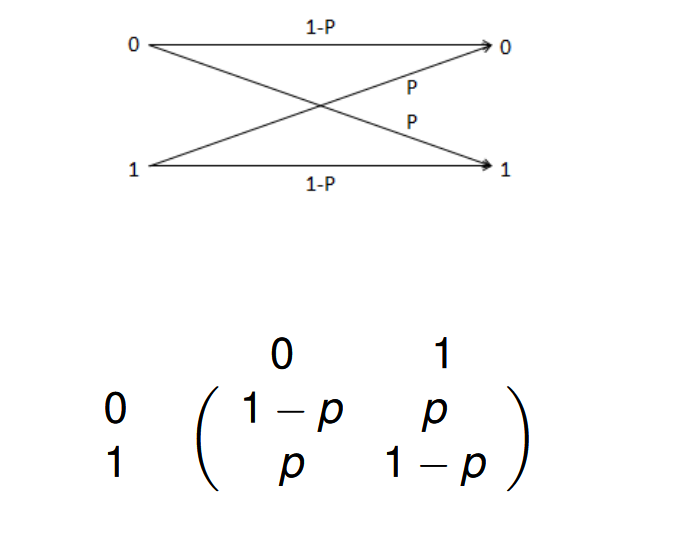
\includegraphics[width=\textwidth]{image/8.png}
    \caption{二元对称信道}
    \label{fig:image1}
  \end{subfigure}
  \hfill
  \begin{subfigure}[b]{0.3\textwidth}
    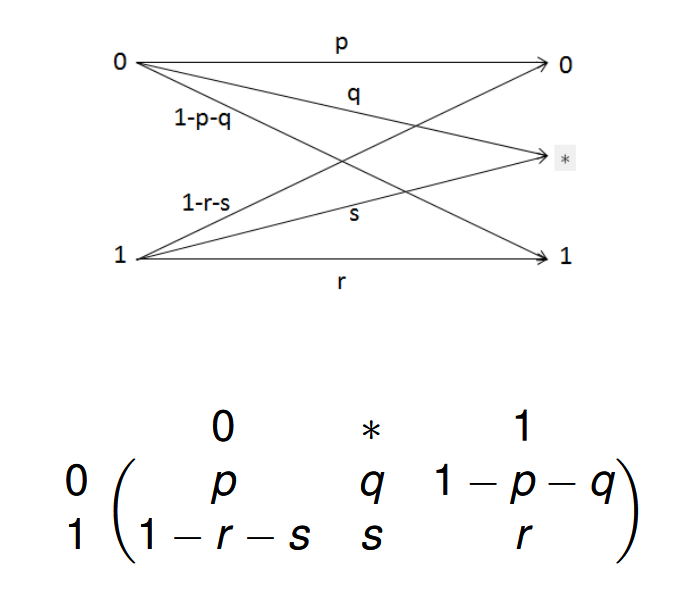
\includegraphics[width=\textwidth]{image/9.png}
    \caption{二元擦除信道}
    \label{fig:image2}
  \end{subfigure}
  \hfill
  \begin{subfigure}[b]{0.3\textwidth}
    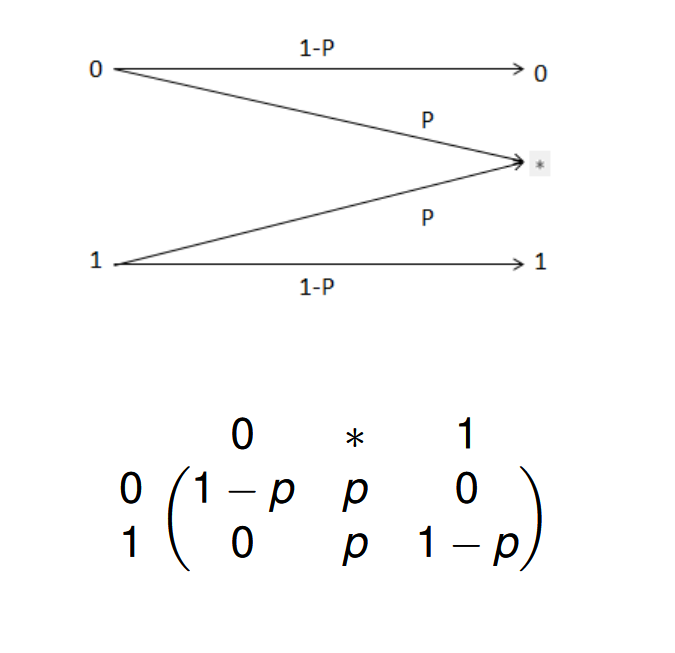
\includegraphics[width=\textwidth]{image/10.png}
    \caption{$ M $ 信道}
    \label{fig:image3}
  \end{subfigure}
  %\caption{}
  \label{fig:three_images}
\end{figure}
\end{solution}

\begin{exercise}
    Z信道如下图所示, 求其信道容量
    \begin{figure}[h]
        \centering
        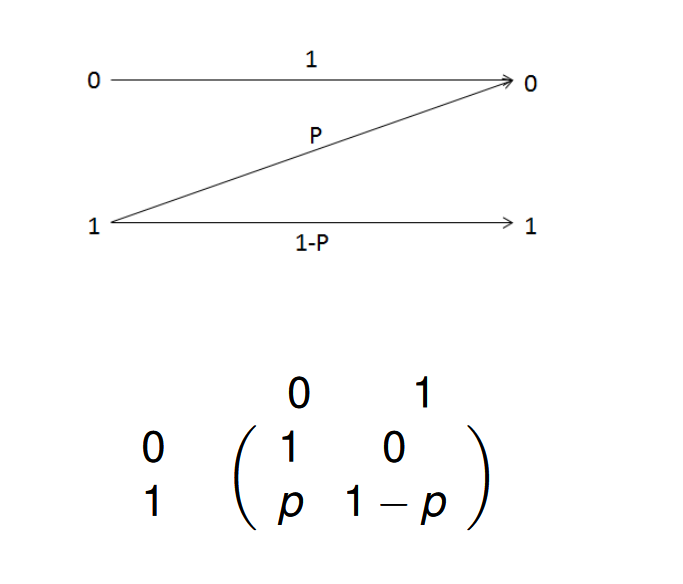
\includegraphics[width=0.4\linewidth]{image/11.png}
    \end{figure}
    \end{exercise}
    \begin{solution}
    根据信道容量的定义有$$C=p(0 \mid 0) \log \frac{p(0 \mid 0)}{q_{0}}+p(1 \mid 0) \log \frac{p(1 \mid 0)}{q_{1}}=p(0 \mid 1) \log \frac{p(0 \mid 1)}{q_{0}}+p(1 \mid 1) \log \frac{p(1 \mid 1)}{q_{1}}$$
$$
\begin{aligned}
\text{左边}&=\log \frac{1}{q_{0}}, \\
\text{右边}&=p \log \frac{p}{q_{0}}+(1-p) \log \frac{1-p}{q_{1}} \\
&=p \log p-p \log q_{0}+(1-p) \log (1-p)-(1-p) \log q_{1} \\
&=-H(p)-p \log q_{0}-(1-p) \log q_{1} .
\end{aligned}
$$
$$\left(q_{0}, q_{1}\right)=(\theta, 1-\theta)\left(\begin{array}{cc}1 & 0 \\ p & 1-p\end{array}\right)=(\theta+p(1-\theta),(1-\theta)(1-p))$$


$$ \begin{aligned}-\log q_{0}+p \log q_{0}+(1-p) \log q_{1}&=-H(p) \\ (1-p) \log q_{0}+(p-1) \log q_{1}&=H(p) \\ (1-p) \log \frac{q_{0}}{q_{1}}&=H(p)\\\log \frac{q_{0}}{q_{1}}&=\frac{H(p)}{1-p} \\ \frac{q_{0}}{q_{1}}&=2^{\frac{H(p)}{1-p}} \\ \frac{\theta+p(1+\theta)}{(1-\theta)(1-p)}&=2^{\frac{H(p)}{1-p}} \\ \frac{\theta-1+p(1-\theta)+1}{(1-\theta)(1-p)}&=2^{\frac{H(p)}{1-p}} \\ \frac{(1-\theta)(p-1)+1}{(1-\theta)(1-p)}&=2^{\frac{H(p)}{1-p}}\\-1+\frac{1}{(1-\theta)(1-p)}&=2^{\frac{H(\rho)}{1-p}} \\ \frac{1}{(1-\theta)(1-p)}&=2^{\frac{H(p)}{1-p}}+1 \\ \frac{1}{1-\theta}&=(1-p)\left[2^{\frac{H(p)}{1-p}}+1\right] \\ \theta&=\frac{1}{1-p}\left[-p+\frac{2^{\frac{H(p)}{1-p}}}{1+2^{\frac{H(p)}{1-p}}}\right]\end{aligned} $$
于是
$$ C=\log \frac{1}{\theta+p(1-\theta)}  =\log \frac{1}{\theta(1-p)+p}  =\log \frac{1+2^{\frac{H(p)}{1-p}}}{2^{\frac{H(p)}{1-p}}}=\log \left[1+2^{\frac{-H(p)}{1-p}}\right] . $$
    \end{solution}

\begin{exercise}
考虑离散无记忆信道 $ Y=(X+Z) \bmod 11 $, 其中
$$
Z=\left(\begin{array}{ccc}
1 & 2 & 3 \\
\frac1 3 & \frac1 3 & \frac1 3
\end{array}\right)
$$
$ X \in\{0,1, \cdots, 10\} $. 假设 $ X $ 和 $ Z $ 独立.\\
(1) 求这个信道的容量.\\
(2) 找出达到信道容量的入口分布.
\end{exercise}
\begin{solution}
(1) $ Y=(X+Z) \bmod 11 $, 输入为 $ X $, 输出为 $ Y, Z $ 为噪声信道, 而
$$
Z=\left(\begin{array}{ccc}
1 & 2 & 3 \\
\frac1 3 & \frac1 3 & \frac1  3
\end{array}\right), \quad X \in\{0,1, \cdots, 10\}
$$
所以 $ Y \in\{0,1, \cdots, 10\} $, 

因为 $ Z $ 可以取三个值 $ (1,2,3) $ ,每个都有 $ \frac{1}{3} $ 的概率,所以对于每个 $ X $ 的值, $ Y $ 可以是三个可能的结果之一,这取决于 $ Z $ 的值.信道矩阵 $ P(Y \mid X) $ 将具有 11 行 (对应于 $ X $ 的可能值) 和 11 列(对应于 $ Y $ 的可能值).每个元素 $ P_{i j} $ 表示给定输入 $ X=i $ 时输出 $ Y=j $ 的概率.

由于 $ Z $ 的作用是加在 $ X $ 上然后对 11 取模,每个 $ X $ 值将映射到三个不同的 $ Y $ 值,每个的概率都是 $ \frac{1}{3} $ .例如,如果 $ X=0 $ ,则 $ Y $ 可以是 $ 1 , 2 $ 或 3 ,每个都有 $ \frac{1}{3} $ 的概率,因为 $ Z $ 分别加 $ 1 , 2 $ 或 3 .因此,信道矩阵的一般形式将是每行有三个 $ \frac{1}{3} $ 的条目,分别对应于 $ X $ 加上 $ 1 , 2 , 3 $ 和模 11 的结果,而其他位置为 0 .对于 $ X=0: Y $ 的可能值是 $ 1,2,3 $ ,每个概率为 $ \frac{1}{3} $ . 对于 $ X=1: Y $ 的可能值是 $ 2,3,4 $ ,每个概率为 $ \frac{1}{3} $ .以此类推,直到 $ X=10 $ .每行的具体值会随着 $ X $ 的增加而“滚动”,并在达到 10 并绕回 0 时循环.这种模式的重复构成了完整的信道矩阵:

\begin{figure}[h]
    \centering
    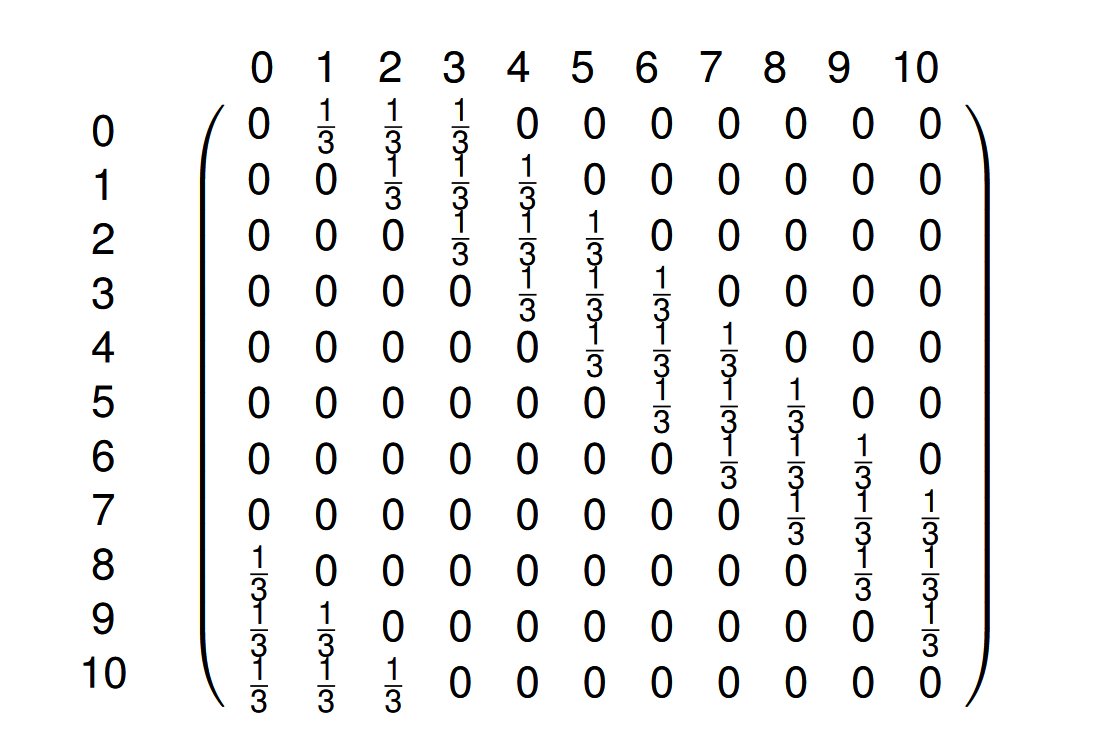
\includegraphics[width=0.6\linewidth]{image/12.png}
\end{figure}
可见 $ Z $ 对输入 $ X $ 的每个取值的作用效果一样, 这是一个对称信道, 因此
$$
\begin{aligned}
C & =\log 11-\left(\frac{1}{3} \log 3+\frac{1}{3} \log 3+\frac{1}{3} \log 3\right) \\
& =\log 11-\log 3=\log \frac{11}{3} .
\end{aligned}
$$

(2) 对于对称信道,最大化信道容量的输入分布是等概率分布. ,即
$$
p(X)=\frac{1}{11}, \quad, X \in\{0,1, \cdots, 10\} .
$$
\end{solution}

这个等概率分布的选择反映了信息论中的一个基本原则:当所有可能的事件(在这个情况下是输入信号的选择)都具有相同的概率时,不确定性(和因此信息熵)最大.在一个对称信道中,由于所有的输入对输出的影响是相同的,等概率分布确保了输出分布也尽可能均匀,从而最大化了从输入到输出的信息传递.

\chapter{抽象代数的基本知识}
\section{群}
\subsection{群的概念}

\begin{definition}
    设 $ G \times G \rightarrow G $ 是 $ G $ 上的一个二元运算, 若"$\cdot$ "满足
    
(1) $ \forall a, b, c \in G,(a \cdot b) \cdot c=a \cdot(b \cdot c) $;

(2) $ \exists e \in G $, 有 $ a \cdot e=e \cdot a=a $;

(3) $ \forall a \in G, \exists a^{-1} \in G $, 有 $ a \cdot a^{-1}=a^{-1} \cdot a=e $.

则称 $ G $ 关于二元运算“. "作成一个群. $ a \cdot b $ 简记作 $ a b $.
\end{definition}
\begin{example}
    $ (\mathrm{Z},+) $, 单位元0, $ \forall a \in Z,-a=a^{-1} $.
\end{example}

\begin{example}
 $ \left(\mathrm{Z}_{p}^{*}, \odot\right) $, 单位元 $ 1, \mathrm{Z}_{p}^{*}=\{1,2, \cdots, p-1\} $. $p$为素数.
 
 $ a \odot b=a b(\bmod p) $, 若 $ (a, p)=1 $ 即 $ \exists s, t $, 使得 $ a s+p t=1 $ , 因此$ as\equiv 1(\bmod p) $,故 $ a^{-1}=s $. 则 $ \left(\mathrm{Z}_{p}, \odot\right) $ 是一个群.
$$
a \oplus b=(a+b)(\bmod p)
$$
$\mathrm{Z}_{p}=\{0,1,2, \cdots, p-1\}$, 根据上面的定义$(Z_p,\oplus)$构成一个含有$p$个元素的交换群.

\begin{remark}
    $ G $ 是一个群, 若对 $ \forall a, b \in G $, 有 $ a b=b a $, 则 $ G $ 为交换群 (Abel群,加法群)
    
此时: $ a \cdot b=a+b $, $a^{n}=a+a+\cdots+a=n a$, $ 0 \cdot a=0 $, 单位元用 0 表示
\end{remark}
\end{example}

\subsection{子群及判定}
\begin{definition}
    设 $ G $ 是一个群, $ S \subseteq G, S \neq \emptyset $, 若 $ S $ 关于 $ G $ 的运算也构成一个群,则称 $ S $ 是 $ G $ 的子群.
\end{definition}
如: $ S=\{n k \mid \forall k \in Z, n $ 是固定的整数 $ \} $

\textbf{ 判定1:} 设 $ G $ 是一个群, $ S \subseteq G, S \neq \emptyset $, 若 $ S $ 满足 :\\
(1) $ \forall a, b \in S, a b \in S $;
(2) $ \forall a \in S $, 有 $ a^{-1} \in S $;则称 $ S $ 是 $ G $ 的子群.

\textbf{判定2: }设 $ G $ 是一个群, $ S \subseteq G, S \neq \emptyset $, 若对 $ \forall a, b \in S $,有 $ a b^{-1} \in S $, 则称 $ S $ 是 $ G $ 的一个子群.
\subsection{群中元素的阶}
\begin{definition}
    设 $ G $ 是一个群, $ a \in G $, 使得 $ a^{m}=e $ 的最小正整数 $ m $ 称为 $ a $ 的阶, 记作 $ o(a)=m $ 或 $ |a|=m $, 若这样的正整数 $ m $ 不存在, 则称 $ a $ 的阶为无穷大 (无限的).
\end{definition}
\begin{example}
 $ (\mathrm{Z},+), \forall a \in \mathrm{Z}, a \neq 0, a $ 的阶无限.
$ G=\left\{A=\left(a_{i j}\right)_{2 \times 2} \mid A\right. $ 可逆, $ \left.a_{i j} \in \mathrm{R}\right\} $, 则 $ G $ 关于乘法构成群,
$$
T=\left(\begin{array}{ll}
0 & 1 \\
1 & 0
\end{array}\right) \in G \quad T^{2}=E, \quad o(T)=2 .
$$
\end{example}
性质:

(1) 设 $ o(a)=m $, 则 $ a^{n}=e \Leftrightarrow m \mid n $;

(2) $ o(a)=m, o(b)=n $, 且有 $ a b=b a $, 若 $ (m, n)=1 $,则 $ o(a b)=m n $;

(3) $ o(a)=m $, 则 $ o\left(a^{k}\right)=\frac{m}{(m, k)} $,
且 $ O\left(a^{k}\right)=m \Leftrightarrow(k, m)=1 $ ( $ k $ 为正整数).

\subsection{循环群}
\begin{definition}
设 $ G $ 是一个群, $ o(a)=n $, 若 $ G=\left\{e, a, a^{2}, \cdots, a^{n-1}\right\} $,则称 $ G $ 为 $ n $ 阶循环群.
 若$o(a)  =\infty$,  则$G=\left\{e, a^{ \pm 1}, a^{ \pm 2}, \cdots, a^{ \pm n}, \cdots,\right\} =\left\{a^{n} \mid n \in Z\right\}$,  则称 $ G$ 为无限阶循环群, 记作$ G=\langle a\rangle$ .
\end{definition}
\begin{example}
     $ (\mathrm{Z},+) $ 是无限循环群; $ \left(\mathrm{Z}_{n}, \oplus\right) $ 为 $ n $ 阶循环群.
\end{example}
\textbf{结论: 循环群的子群也是循环群.}

\section{环与域}
\subsection{环的概念}
\begin{definition}
    $ R \neq \emptyset,+ $, 满足\\
(1) $ R $ 对加法构成一个交换群; 0 是零元;\\
(2) $ \forall a, b, c \in R,(a b) c=a(b c) $;\\
(3)
$a(b+c)=a b+a c ,(b+c) a=b a+c a .$\\
则称 $ R $ 关于二元运算,+ , 运算构成一个环, 记作 $ (R,+, \cdot) $.\\若对 $ \forall a, b \in R $, 有 $ a b=b a $,则称 $ R $ 为交换环.
\end{definition}
\begin{example}
    $ (\mathrm{Z},+, \cdot),(\mathrm{Q},+, \cdot),(\mathrm{R},+, \cdot) $ 都是交换环.(无限)
\end{example}
 
\begin{example}
    $ \left(\mathrm{Z}_{n}, \oplus, \odot\right) $ 构成一个交换环.(有限)
$$
a \oplus b=(a+b)(\bmod n) \quad
a \odot b=a b(\bmod n)
$$
\end{example}

\subsection{域}
\begin{definition}
    $ R $ 是一个交换环, $ R^{*}=\{a \in R \mid a \neq 0\} $, 若 $ R^{*} $ 关于环 $ R $ 的乘法运算作成一个交换群,则称 $ R $ 为一个域.加法的单位元称为零元 $ 0, R^{*} $ 乘法的单位元 1 .
\end{definition}
\begin{example}
    $ (\mathrm{Q},+, \cdot),(\mathrm{R},+, \cdot) $ 都是域. $ \left(\mathrm{Z}_{n}, \oplus, \odot\right) $ 是域 $ \Leftrightarrow n=p(p $ 是素数 $ ) $
\end{example}
\begin{definition}
    设 $ (R,+, \cdot) $ 是环, $ (F,+, \cdot) $ 是域,\\
(1) $ R_{1} \subseteq R, R_{1} \neq \emptyset $, 若 $ R_{1} $ 构成一个环, 则称 $ R_{1} $ 为 $ R $ 的子环, $ R $ 称为 $ R_{1} $ 的扩环.\\
(2) $ F_{1} \subseteq F, F_{1} \neq \emptyset $,若 $ F_{1} $ 构成一个域,则称 $ F_{1} $ 为 $ F $ 的子域, $ F $ 称为 $ F_{1} $ 的扩域.
\end{definition}
\begin{theorem}
    设 $ (R,+, \cdot) $ 为环, $ (F,+, \cdot) $ 为域, 则\\
(1) $ R_{1} $ 为 $ R $ 的子环 $ \Leftrightarrow \forall a, b \in R_{1}, a-b \in R_{1}, a \cdot b \in R_{1} $;\\
(2) $ F_{1} $ 为 $ F $ 的子域 $ \Leftrightarrow \forall a, b \in F_{1}, a-b \in F_{1}, a b^{-1} \in F_{1} $.
\end{theorem}

\section{ 理想和商环}
\subsection{理想}
\begin{definition}
    设 $ / $ 是环 $ R $ 的子环, 若对 $ \forall a \in I, x \in R $, 有 $ a \cdot x \in I $, $ x \cdot a \in I $, 则称 $ l $ 是 $ R $ 的理想.
\end{definition}
\begin{example}
    $ (\mathbb{Z},+, \cdot) \quad I=\{n k \mid k \in \mathbb{Z}, n $ 是固定整数 $ \}, l $ 是 $ \mathbb{Z} $ 的理想.平凡理想: $ \{0\}, R $.
\end{example}

 \textbf{判定:}设 $ (R,+, \cdot) $ 是一个环 $ , I \subseteq R, I \neq \emptyset, I $ 是 $ R $ 的理想 $ \Leftrightarrow $\\
(1) $ \forall a, b \in I, a-b \in l $;\\
(2) $ \forall a \in I, x \in R $, 有 $ a \cdot x \in I, x \cdot a \in I $.
\begin{definition}
    设 $ (R,+, \cdot) $ 为环, $ a \in R, R $ 的包含 $ a $ 的最小理想称为由 $ a $ 生成的主理想, 记作 $ \langle a\rangle $.
\end{definition}

\begin{theorem}
    若 $ (R,+, \cdot) $ 是有单位元的交换环, 则 $ \langle a\rangle=\{r a \mid \forall r \in R\} $.
\end{theorem}

\subsection{商环}
\begin{definition}
    设 $ (R,+, \cdot) $ 为一个环, $ l $ 是 $ R $ 的一个理想, 定义 $ a+I=\{a+i \mid \forall i \in I\} $,称为 $ / $ 的一个陪集, $ a $ 为代表元.记 $ R / I=\{a+I \mid \forall a \in R\} $
\end{definition}
\begin{remark}

    (1) $ a+I=b+I \Leftrightarrow a-b \in I $;
    
(2) $ a+1 $ 与 $ b+1 $ 要么相等,要么交为 $ \emptyset $.
\end{remark}
\begin{definition}
    在 $ R / I $ 上定义两个二元运算:\\
(1) $ (a+I) \oplus(b+l)=(a+b)+l $;\\
(2) $ (a+l) \odot(b+l)=a b+l $;\\
则 $ R / I $ 关于定义的 $ \oplus, \odot $ 作成一个环,称为商环.
\end{definition}

\subsection{环(域)的同构}

设 $ R, S $ 是两个环(或域), 若存在一个 $ 1-1 $ 映射 $ f: R \rightarrow S $ 满足:\\
(1) $ \forall a, b \in R $, 有 $ f(a+b)=f(a)+f(b) $;\\
(2) $ \forall a, b \in R $, 有 $ f(a b)=f(a) f(b) $;则称 $ f $ 为同构映射,此时称 $ S $ 与 $ R $ 同构,记作 $ R \cong S $.
\begin{example}
    $ (\mathrm{Z},+, \cdot) $ 是环, $ I=\{n k \mid \forall k \in Z, n $ 为固定整数 $ \} $,则: $ \mathrm{Z} / I \cong\left(\mathrm{Z}_{n}, \oplus, \odot\right) $
    $$
\begin{aligned}
f: \mathrm{Z}_{n} & \rightarrow \mathrm{Z} / I \\
\quad x & \mapsto x+I \\
f(x) & =f(y) \Rightarrow x+I=y+I \Rightarrow x-y \in I,
\end{aligned}
$$
即 $ x-y=n k_{1}, n \mid x-y \Rightarrow x=y $
$ f $ 是单射,显然 $ f $ 是满射.
$$
\begin{array}{l}
f(x+y)=(x+y)+I=(x+I)+(y+I)=f(x)+f(y) \\
f(x \cdot y)=(x \cdot y)+I=(x+I) \cdot(y+I)=f(x) \cdot f(y)
\end{array}
$$
故 $ f $ 为同构映射.
\end{example}

\section{域上的产项式环}

\subsection{域上的多项式环}

\textbf{1.域上的多项式} 

$ (F,+, \cdot) $ 是一个域, $ x $ 是一个文字(未定元), 称 $ a_{n} x^{n}+a_{n-1} x^{n-1}+\cdots+a_{1} x+a_{0} $,\\$\left(a_{i} \in F, i=0,1, \cdots, n\right) $为域 $ F $ 上的一元多项式, 若 $ a_{n} \neq 0 $, 定义 $ \operatorname{deg}(f(x))=n, a_{n} $ 为首项系数.

\textbf{2. 域上的多项式环}

记 $ F[x]=\left\{a_{n} x^{n}+a_{n-1} x^{n-1}+\cdots+a_{1} x+a_{0} \mid\left(a_{i} \in F, i=0, \cdots, n\right)\right\} $, 在 $ F $ 上定义,$ + \cdot $, 则 $ F[x] $ 构成一交换环(不是域).

\subsection{带余除法}
\begin{theorem}
    $ f(x), g(x) \in F[x], \exists $ 唯一的 $ q(x), r(x) $ 有
$$
f(x)=g(x) q(x)+r(x)
$$
其中 $ \partial(r(x))<\partial(g(x)) $ 或 $ r(x)=0 $, 记 $ r(x)=[f(x)]_{g(x)} $
\end{theorem}
\begin{definition}[同余]
    $ a(x), b(x), p(x) \in F[x] $, 若 $ p(x) \mid a(x)-b(x) $, 则称 $ a(x) $ 与 $ b(x) $ 模 $ p(x) $ 同余,记作 $ a(x) \equiv b(x)(\bmod p(x)) $.
\end{definition}
\begin{example}
    $ F=F_{2}=\{0,1\} $, 取 $ a(x)=x^{5}+x^{4}+x^{2}+1 $,$b(x)=x^{3}+x+1$,则 $ q(x)=x^{2}+x+1, r(x)=x^{2} $.
\end{example}

\subsection{最大公因式与最小公倍式}

1.最大公因式;

2. 求法: 辗转相除法;

3.互素;

4. 最小公倍式.
\subsection{不可约多项式}
\begin{definition}
    $ p(x) \in F[x], \operatorname{deg}(p(x)) \geqslant 1 $, 若 $ p(x) $ 的因式只能为 $ a \in F $或 $ c p(x) $,则称 $ p(x) $ 为不可约多项式,否则称其为可约多项式.
\end{definition}
\textbf{性质:}

(1) $ p(x) $ 不可约, $ p(x) \mid a(x) b(x) $, 则有 $ p(x) \mid a(x) $ 或 $ p(x) \mid b(x) $;

(2) $ p(x) $ 不可约,则对 $ \forall a(x) \in F[x] $, 有 $ p(x) \mid a(x) $ 或 $ (p(x), a(x))=1 $;

\textbf{标准分分解式:}
$ f(x) \in F[x], \partial(f(x)) \geqslant 1 $,则 $ f(x) $ 可以唯一地表示成
$$
f(x)=b p_{1}(x)^{k_{1}} \cdots p_{s}(x)^{k_{s}}
$$
其中 $ p_{i}(x)(i=1, \cdots, s) $ 为不可约多项式, 且首项系数为 1 .



\subsection{不可约多项式与有限域的构造}

设 $ p(x) $ 为不可约多项式, $ \langle p(x)\rangle=\{p(x) a(x) \mid \forall a(x) \in F[x]\} $, $ \operatorname{deg}(p(x))=n, F[x] /\langle p(x)\rangle $ 是商环, $ \forall f(x) \in F[x] $, $ f(x)=g(x) p(x)+r(x)(\partial(r(x))<\partial(p(x)) $ 或 $ r(x)=0) $,记 $ F[x]_{p(x)}=\left\{a_{0}+a_{1} x+\cdots+a_{n-1} x^{n-1} \mid \forall a_{i} \in F, i=0, \cdots, n-1\right\} $,则 $ F[x]_{p(x)} $ 关于下述定义的加法和乘法作成一个交换环, $$ a(x) \oplus b(x)=a(x)+b(x) $$
$$
a(x) \odot b(x)=(a(x) \cdot b(x))_{p(x)}
$$
则 $ F[x] /\langle p(x)\rangle \cong F[x]_{p(x)} $
\begin{proof}
    $$ \begin{aligned} \varphi: & F[x] /\langle p(x)\rangle \rightarrow F[x]_{p(x)} \\ & f(x)+p(x) \mapsto(f(x))_{p(x)}\end{aligned} $$
    $$
\begin{array}{c}
\varphi(f(x)+\langle p(x)\rangle+g(x)+\langle p(x)\rangle)=\varphi(f(x)+g(x)+\langle p(x)\rangle) \\
=(f(x)+g(x))_{p(x)}=(f(x))_{p(x)}+(g(x))_{p(x)}
\end{array}
$$
$ \varphi $ 是一个同构映射.

$ F[x] /\langle p(x)\rangle $ 是域 $ \Leftrightarrow p(x) $ 不可约;
$ F[x]_{p(x)} $ 是域 $ \Leftrightarrow p(x) $ 不可约;
$ \forall a(x) \in F[x]_{p(x)}, a(x) \neq 0 $, 即 $ a(x) \nmid p(x),(a(x), p(x))=1 $.
$ (a(x), p(x))=1 \Leftrightarrow \exists u(x), v(x) $ 有 $ a(x) u(x)+p(x) v(x)=1 $
$ \Leftrightarrow $ 有 $ (a(x) u(x))_{p(x)}=1, a(x)^{-1}=u(x) $.
故 $ F[x]_{p(x)} $ 是一个域, 即 $ F[x] /\langle p(x)\rangle $ 是一个域.
\end{proof}

$ F[x]_{p(x)}=\left\{a_{0}+a_{1} x+\cdots+a_{n-1} x^{n-1} \mid \forall a_{i} \in F, i=0, \cdots, n-1\right\} $,

若 $ |F|=q $, 则 $ \left|F[x]_{p(x)}\right|=q^{n} $; 特别地 $ |F|=p $, 则 $ \left|F[x]_{p(x)}\right|=p^{n} $.
\begin{example}
    $ p(x)=x^{2}+x+1, p(x) $ 是 $ F_{2} $ 上的不可约多项式, $ F[x]_{p(x)}=\left\{a_{0}+a_{1} x \mid a_{0}, a_{1} \in F_{2}\right\} $ 是域. $ F[x]_{p(x)}=\{0,1,1+x, x\} $
\end{example}

\subsection{重因式及多项式的根}
$ p(x)=x^{2}+x+1,0,1 $ 不是 $ p(x) $ 的根.

\section{有限域}
\subsection{有限域}
\begin{definition}
    设 $ F $ 是一个域,若 $ F $ 含有限个元素,则称 $ F $ 为有限域, 若 $ |F|=q $, 则记为 $ F_{q} $.
\end{definition}
\begin{example}
    $ \left(\mathrm{Z}_{p}, \oplus, \odot\right), \mathrm{Z}_{p}=\{0,1,2, \cdots, p-1\}, p $ 为素数, 构成一个有限域.
$$ a \oplus b=(a+b)(\bmod p) $$
$$ a \odot b=a b(\bmod p) $$
若 $ p $ 不是素数, 则 $ Z_{p} $ 不是域.
\end{example}
\subsection{域的特征}
\begin{definition}
    设 $ F $ 是一个域, $ e $ 为 $ F $ 的单位元, 若对任意的正整数 $ m $, 有 $ m e \neq 0 $, 则称 $ F $ 的特征为 0 ; 若存在正整数 $ m $, 有 $ m e=0 $, 则满足该条件的最小正整数称为 $ F $ 的特征.
\end{definition}
\begin{example}
    $ \mathrm{Q}, \mathrm{R}, \mathrm{C} $ 的特征为 $ 0, \mathrm{Z}_{p} $ ( $ p $ 为素数)特征为 $ p $.
\end{example}

\textbf{性质 1 :}设 $ F $ 为有限域,则 $ F $ 的特征为素数.
\begin{proof}
    设 $ p $ 为 $ F $ 的特征,假设 $ p $ 不是素数,则$p=p_{1} p_{2}\left(p_{1}<p, p_{2}<p\right)$, 于是$ p e=p_{1} p_{2} e=\left(p_{1} e\right)\left(p_{2} e\right)=0 $ $\Rightarrow p_{1} e=0 \text { 或 } p_{2} e=0, \text { 而 } p_{1}<p, p_{2}<p$
,与 $ p $ 是 $ F $ 的特征矛盾,故 $ p $ 为素数.
\end{proof}


\textbf{性质2: }设 $ F $ 为有限域, 若 $ F $ 的特征为 $ p $, 则对 $ \forall a \in F, a \neq 0 $,
有 $ p a=0 $ 且 $ p $ 为 $ a $ 的加法阶.

\begin{proof}
    设 $ p $ 为 $ F $ 的特征,则有 $ p e=0 $ ,
对 $ \forall a \in F, a \neq 0, a=a \cdot e=e \cdot a $
则有 $ p a=p e \cdot a=0 \cdot a=0 $.
假设 $ o(a)=m $, 则 $ m<p $, 有 $ m a=0 $, 
$ 0=m a=m e a=(m e) a $, $ a \neq 0 \Rightarrow m e=0 $ ,而 $ m<p $ 与 $ p $ 是 $ e $ 的阶矛盾,
故对 $ \forall a \in F, a \neq 0, p a=0 $.
\end{proof}

\subsection{素域}
\begin{definition}
    设 $ F $ 为有限域, 称 $ F $ 的最小子域为 $ F $ 的素域, 即 $ F $ 的素域是 $ F $ 的所有子域的交集.
\end{definition}

设 $ p $ 是有限域 $ F $ 的特征, 记 $ \pi=\{0, e, 2 e, \cdots,(p-1) e\} $则 $ \pi $ 是 $ F $ 的最小子域, 事实上, 对 $ \forall a, b \in \pi $,
$$
\begin{array}{l}
\quad a=k e, b=\ell e, \ell \neq 0 \\
a-b=k e-\ell e=(k-\ell) e=(k-\ell)(\bmod p) e \in \pi \\
a b^{-1}=k \ell^{-1} e=k \ell^{-1}(\bmod p) e \in \pi
\end{array}
$$
而 $ e $ 含于 $ F $ 的任意子域,故 $ \pi $ 含于 $ F $ 的任一子域中,即 $ \forall F_{1} $ 为 $ F $ 的子域, $ \pi \subseteq F_{1} $, 从而 $ \pi $ 是 $ F $ 的素域.

事实上, 因 $ \pi $ 包含于 $ F $ 的任一子域, 不妨设为 $ F_{1}, F_{2}, \cdots, F_{n} $, 故 $ \pi \subseteq \bigcap\limits_{i=1}^{n} F_{i} $, 又 $ \pi \subseteq \bigcap\limits_{i=1}^{n} F_{i} $ 为 $ F $ 的最小子域, 而 $ \pi $ 是 $ F $ 的子域, 不妨设 $ \pi=F_{j} $, 故 $ \bigcap\limits_{i=1}^{n} F_{i} \subseteq \pi $, 故 $ \pi=\bigcap\limits_{i=1}^{n} F_{i} $.

结论:
$$
\begin{aligned}
\pi \cong \mathrm{Z}_{p}&=\{0,1,2, \cdots, p-1\}\\
f: \mathrm{Z}_{p} & \rightarrow \pi \\
k & \mapsto k e
\end{aligned}
$$

\subsection{有限域 $ F_{q} $ 的性质}
\textbf{运算性质:}

(1) 设 $ p $ 是有限域 $ F $ 的特征, 则 $ (a \pm b)^{p}=a^{p} \pm b^{p} $.
\begin{proof}
    $$ (a+b)^{p}=a^{p}+b^{p}+\sum_{i=1}^{p-1} C_{p}^{i} a^{i} b^{p-i} $$
下面证明 $ p \mid C_{p}^{i} ,\quad C_{p}^{i}=\frac{p !}{(p-i) ! i !} $.
即 $ p !=C_{p}^{i}(p-i) ! i ! \quad p \nmid(p-i) ! , p \nmid i ! $,
故 $ p \nmid(p-i) ! i !(p $ 是素数).
而 $ p \mid p $ !,即 $ p \mid C_{p}^{i}(p-i) ! i ! $ , 故 $ p \mid C_{p}^{i} $.
从而 $ C_{p}^{i} a^{i} b^{p-i}=0 $ 成立.
\end{proof}

(2)设 $ p $ 是有限域 $ F $ 的特征, 则 $ \left(\sum\limits_{i=1}^{m} a_{i}\right)^{p}=\sum\limits_{i=1}^{m} a_{i}^{p} $,$(a \pm b)^{p^{n}}=a^{p^{n}} \pm b^{p^{n}} .$

\begin{lemma}
    设 $ (G, \cdot) $ 有限交换群, $ n $ 是 $ G $ 中所有元素阶数的最大值, 则 $ G $ 中所有元素的阶数是 $ n $ 的因子.
\end{lemma}
\begin{proof}
    设 $ a \in G, a $ 的阶为 $ n $, 即 $ a^{n}=e $,对 $ \forall b \in G $, 设 $ b $ 的阶为 $ m $, 证明 $ m \mid n $, 假设 $ m \nmid n $
$$
m=p_{1}^{e_{1}} p_{2}^{e_{2}} \cdots, p_{s}^{e_{s}}, n=p_{1}^{e_{1}^{\prime}} p_{2}^{e_{2}^{\prime}} \cdots, p_{s}^{e_{s}^{\prime}}
$$
$ m \nmid n $, 则一定存在 $ p_{i} $, 有 $ e_{i}>e_{i}^{\prime} $
不妨设为 $ p_{1} $, 即 $ e_{1}>e_{1}^{\prime} $
$$
\text { 令 } m=p_{1}^{e_{1}} m_{1}, \quad n=p_{1}^{e_{1}^{\prime}} n_{1}
$$
$$
e_{1}>e_{1}^{\prime} \quad\left(p_{1}, m_{1}\right)=1 \quad\left(p_{1}, n_{1}\right)=1
$$
$ a^{p_{1}^{e_{1}^{\prime}}} $ 的阶数为 $ \frac{n}{\left(n, p_{1}^{e_{1}^{\prime}}\right)}=\frac{n}{p_{1}^{e_{1}^{\prime}}}=n_{1} $, 又 $ \left(n_{1}, p_{1}^{e_{1}}\right)=1 $
\end{proof}

\begin{theorem}
    设 $ F $ 为有限域, $ F^{*}=F \backslash\{0\} $, 则 $ \left(F^{*}, \cdot\right) $ 是一个循环群.
\end{theorem}
\begin{proof}
设 $ n $ 是 $ F^{*} $ 中元素的最大阶,则对 $ \forall a \in F^{*}, o(a) \mid n $,故对 $ \forall a \in F^{*}, a^{n}=1 $.
设 $ \alpha \in F^{*}, \alpha $ 的阶数为 $ n $, 令 $ \langle\alpha\rangle=G=\left\{1, \alpha, \alpha^{2}, \cdots, \alpha^{n-1}\right\} $, 下面证明 $ G=F^{*}=\langle\alpha\rangle $. 设 $ |F|=q $,则 $ \left|F^{*}\right|=q-1, G \subseteq F^{*} $,故 $ q-1 \geqslant n $;又令 $ f(x)=x^{n}-1, f(x) $ 在 $ F $ 上至多有 $ n $ 个根,而 $ \forall a \in F^{*} $, 均有 $ a^{n}=1 $, 即 $ a^{n}-1=0 $,即 $ F^{*} $ 中的 $ q-1 $ 个元素均为 $ f(x) $ 的根, 故有 $ q-1 \leqslant n $,从而 $ q-1=n, F^{*}=G, F^{*} $ 为循环群.
\end{proof}

\begin{definition}
    设 $ F $ 为有限域, 乘法群 $ F^{*} $ 的生成元称为 $ F $ 的本原元.
\end{definition}

\begin{theorem}
    设 $ F_{1} $ 是有限域 $ F $ 的子域, 并且 $ \left|F_{1}\right|=q $, 则一定存在正整数 $ n $, 使得 $ |F|=q^{n} $.
\end{theorem}
\begin{proof}
设 $ F_{1}=F $, 则结论显然成立.

若 $ F_{1} \subset F, \exists e_{1} \in F $, 但 $ e_{1} \notin F_{1} $,$\text { 令 } F_{2}=\left\{a_{1}+a_{2} e_{1} \mid a_{1}, a_{2} \in F_{1}\right\},\left|F_{1}\right|=q \text {, 故 }\left|F_{2}\right|=q^{2} ,$
事实上,只需说明 $ a_{1}+a_{2} e_{1}=b_{1}+b_{2} e_{1} $
$\left(b_{1}, b_{2}, a_{1}, a_{2} \in F_{1}\right)\Leftrightarrow a_{1}=b_{1}, a_{2}=b_{2} \text { 即可. }$
$$
a_{1}+a_{2} e_{1}=b_{1}+b_{2} e_{1} \Rightarrow\left(a_{1}-b_{1}\right)+\left(a_{2}-b_{2}\right) e_{1}=0
$$
即 $ \left(a_{2}-b_{2}\right) e_{1}=b_{1}-a_{1} \Rightarrow $
$ \left(b_{1}-a_{1}\right)\left(a_{2}-b_{2}\right)^{-1}=e_{1} \in F_{1} $ 矛盾;

若 $ F_{2} \neq F, \exists e_{2} \in F $ 但 $ e_{2} \notin F_{2} $
$\text { 令 } F_{3}=\left\{a_{1}+a_{2} e_{1}+a_{3} e_{2} \mid a_{1}, a_{2}, a_{3} \in F_{1}\right\} \text {, 则 }\left|F_{3}\right|=q^{3} \text {; }$
依次下去,因 $ F $ 是有限域,故必存在 $ n $ 使得 $ |F|=q^{n} $.
\end{proof}

\begin{corollary}
    设 $ p $ 为有限域 $ F $ 的特征, 则必存在正整数 $ n $, 使得 $ |F|=p^{n} $.
\end{corollary}
\begin{proof}
     $ \pi=\{0, e, 2 e, \cdots,(p-1) e\} $ 为 $ F $ 的子域.
\end{proof}

\begin{theorem}
    任意两个元素个数相同的有限域一定同构.
    $$
\begin{aligned}
f: & \rightarrow F^{\prime} \\
& 0 \mapsto 0^{\prime} \\
& \alpha \mapsto \beta \text { (其中 } \alpha \text { 为 } F^{*} \text { 的本原元, } \beta \text { 为 } F^{* *} \text { 的本原元) }
\end{aligned}
$$
\end{theorem}

\begin{corollary}
     设 $ F $ 是有限域, $ \mathrm{Z}_{p}=\{0,1, \cdots, p-1\}, p $ 为素数, $ p(x) $ 是 $ Z_{p} $ 上的不可约多项式,
     
(1) 如果 $ |F|=p^{n} $,则 $ F \cong Z_{p}[x] /\langle p(x)\rangle $;

(2) 如果 $ |F|=p $, 则 $ F \cong Z_{p} $.
\end{corollary}

\subsection{极小多项式与本原多项式}
\begin{definition}
    设 $ F $ 为有限域, $ F_{q} $ 为 $ F $ 的含有 $ q $ 个元素的子域, $ \alpha \in F, F_{q} $上的以 $ \alpha $ 为根, 并且首项系数为 1 的次数最低的多项式称为 $ \alpha $ 在 $ F_{q} $ 上的极小多项式.
\end{definition}

\begin{theorem}
    设 $ F $ 为有限域, $ F_{q} $ 为 $ F $ 的含有 $ q $ 个元素的子域, $ \alpha \in F $,则 $ \alpha $ 在 $ F_{q} $ 上的极小多项式存在, 是唯一的, 并且是 $ F_{q} $ 上的不可约多项式.
\end{theorem}

\begin{example}
     $ f(x)=x^{2}+x+1 $\\
$ f(x) $ 在 $ F_{2} $ 上不可约(无根), 在 $ F_{4} $ 中有两个根.\\
$ f(x) $ 在 $ \mathrm{R} $ 中不可约, $ \alpha=\frac{-1+\sqrt{3} i}{2} $\\
$ f(\alpha)=0 \quad \alpha \in \mathrm{C} $ 但 $ \alpha \notin \mathrm{R}, f(x) $ 为 $ \alpha $ 在 $ \mathrm{R} $ 上的极小多项式.
\end{example}

\begin{definition}
    
定义:设 $ F $ 为有限域, $ F_{q} $ 为 $ F $ 的含有 $ q $ 个元素的子域, $ f(x) $ 为 $ F_{q} $ 上的不可约多项式. 如果 $ f(x) $ 的根都是 $ F $ 的本原元, 则称 $ f(x) $ 为本原多项式.
\end{definition}

\begin{example}
    $ F_{2}[x] $ 中的4次本原多项式为 $ f(x)=x^{4}+x+1 $; $ F_{2}[x] $ 中的 $ f(x)=x^{3}+x+1 $ 是本原多项式, $ f(x) $ 的根在 $ F_{8} $ 中, 每个根的阶均为 7 .
\end{example}

\begin{theorem}
    设 $ F $ 为有限域, $ F_{q} $ 为 $ F $ 的含有 $ q $ 个元素的子域, $ \alpha $ 是 $ F $ 的本原元, $ |F|=q^{n} $, 则 $ \alpha $ 在 $ F_{q} $ 上的极小多项式为 $ n $ 次多项式
$$
f(x)=(x-\alpha)\left(x-\alpha^{q}\right)\left(x-\alpha^{q^{2}}\right) \cdots\left(\left(x-\alpha^{q^{n-1}}\right)\right)
$$
进一步 $ \alpha, \alpha^{q}, \cdots, \alpha^{q^{n-1}} $ 均为 $ F $ 的本原元.
\end{theorem}
\begin{remark}
    极小多项式不一定是本原多项式.
\end{remark}

\section{域上的线性代数}
\subsection{域上的向量空间}
\begin{definition}
    设 $ F $ 是一个域, $ \mathrm{V} \neq \emptyset $,
$$
\begin{array}{c}
+: V \times V \rightarrow V \\
\cdot: F \times V \rightarrow V
\end{array}
$$
且满足:\\
(1) $ (V,+) $ 是一个交换群;\\
(2) 对 $ \forall a \in F, v_{1}, v_{2} \in V, a\left(v_{1}+v_{2}\right)=a v_{1}+a v_{2} $;\\
(3) 对 $ \forall a_{1}, a_{2} \in F, v \in V,\left(a_{1}+a_{2}\right) v=a_{1} v+a_{2} v $;\\
(4) 对 $ \forall v \in V $,有 $ 1 \cdot v=v $;\\
则称 $ V $ 为 $ F $ 上的向量空间.
\end{definition}

\textbf{ 向量空间的基与维数:}

$ V $ 是域 $ F $ 上的向量空间, $ e_{1}, e_{2}, \cdots, e_{n} \in V $, 若对 $ \forall v \in V $, $ v $ 可唯一地表示为 $ v=c_{1} e_{1}+c_{2} e_{2}+\cdots+c_{n} e_{n} $, 其中 $ c_{i} \in F $, $ i=1,2, \cdots, n $, 则称 $ e_{1}, e_{2}, \cdots, e_{n} $ 为 $ V $ 的一组基, $ V $ 称为 $ F $ 上的 $ n $ 维向量空间.

\textbf{ 线性相关与线性无关:}

设 $ V $ 是域 $ F $ 上的线性空间, $ v_{1}, v_{2}, \cdots, v_{r} \in V $, 如果存在不全为 0 的 $ c_{1}, c_{2}, \cdots, c_{r} $ 使得:
$$
c_{1} v_{1}+c_{2} v_{2}+\cdots+c_{r} v_{r}=0,
$$
则称 $ v_{1}, v_{2}, \cdots, v_{r} $ 为线性相关, 否则 $ v_{1}, v_{2}, \cdots, v_{r} $ 线性无关.
\begin{theorem}
    设 $ V $ 是域 $ F $ 上的 $ n $ 维向量空间,则 $ V $ 的任意一组基都是线性无关的.
\end{theorem}
\begin{proof}
    设 $ e_{1}, \cdots, e_{n} $ 是 $ V $ 的一组基,假设 $ e_{1}, e_{2}, \cdots, e_{n} $ 线性相关,则存在不全为 0 的 $ c_{1}, c_{2}, \cdots, c_{n} $, 使得:
$$
c_{1} e_{1}+c_{2} e_{2}+\cdots+c_{n} e_{n}=0
$$
$ 0 e_{1}+0 e_{2}+\cdots+0 e_{n}=0 $ ( 0 向量有两种表达形式)与 $ e_{1}, e_{2}, \cdots, e_{n} $ 是基矛盾.
\end{proof}

\begin{example}
    $ V(n, q)=\left\{\left(a_{1}, a_{2}, \cdots, a_{n}\right) \mid a_{i} \in F_{q}, i=1,2, \cdots, n\right\} $, $ F_{q} $ 为 $ q $ 元有限域.
    
$ a=\left(a_{1}, \cdots, a_{n}\right), b=\left(b_{1}, \cdots, b_{n}\right)  $ .定义:
$ a+b=\left(a_{1}+b_{1}, \cdots, a_{n}+b_{n}\right) \in V(n, q) $\\
$ \lambda \cdot a=\left(\lambda a_{1}, \cdots, \lambda a_{n}\right) \in V(n, q) \quad\left(\lambda \in F_{q}\right) $. 
$ e_{i}=(0, \cdots, 0,1,0, \cdots, 0) i=1, \cdots, n $ 是它的一组基,
$ \forall a \in V(n, q), a=\left(a_{1}, \cdots, a_{n}\right), a=\sum\limits_{i=1}^{n} a_{i} e_{i} $. 
$ V(n, q) $ 为 $ F_{q} $ 上的 $ n $ 维向量空间.
\end{example}

\begin{theorem}
    设 $ F_{q} $ 是有限域 $ F $ 的含 $ q $ 个元素的子域,且 $ |F|=q^{n} $,则 $ F $ 是 $ F_{q} $ 上的 $ n $ 维向量空间.
\end{theorem}
\begin{proof}
    设 $ \alpha $ 是 $ F $ 的本原元, $ \alpha $ 在 $ F_{q} $ 上的极小多项式为 $ g(x) $ (不可约). $ |F|=q^{n} $, 所以 $ \operatorname{deg}(g(x))=n\left(F \cong F_{q}[x] /\langle g(x)\rangle\right) $. 下面证明 $ 1, \alpha, \alpha^{2}, \cdots, \alpha^{n-1} $ 是 $ F $ 的一组基.首先证 $ 1, \alpha, \alpha^{2}, \cdots, \alpha^{n-1} $ 线性无关;假设存在不全为 0 的 $ c_{0}, c_{1}, \cdots, c_{n-1} \in F_{q} $ 使得:
    $$
\begin{array}{c}
c_{0}+c_{1} \alpha+c_{2} \alpha^{2}+\cdots+c_{n-1} \alpha^{n-1}=0 \\
\text { 令 } f(x)=c_{0}+c_{1} x+c_{2} x^{2}+\cdots+c_{n-1} x^{n-1},
\end{array}
$$
则 $ f(x) \in F_{q}[x] $ 并且有 $ f(\alpha)=0 $,
因此 $ g(x) \mid f(x) $ (极小多项式必整除零化多项式), $ f(x) \neq 0 $且 $ \operatorname{deg}(f(x))=n-1<\operatorname{deg}(g(x))=n $与 $ g(x) $ 是极小多项式矛盾.

下证 $ F $ 的任一元素可由其线性表示. $ \alpha $ 是 $ F $ 的本原元, 并且 $ |F|=q^{n} $, 则有:
$$
\begin{array}{l}
\quad F=\left\{0,1, \alpha, \alpha_{2}, \cdots, \alpha^{q^{n}-2}\right\} \\
\text { 设 } x^{i}=q(x) g(x)+r(x), \quad q(x), r(x) \in F_{q}[x], \\
\operatorname{deg}(r(x))<\operatorname{deg}(g(x))=n, i=0,1, \cdots, q^{n}-2,
\end{array}
$$
于是有 $ \alpha^{i}=r(\alpha) $
$$
\text { 设 } r(x)=r_{0}+r_{1} x+r_{2} x^{2}+\cdots+r_{n-1} x^{n-1} r_{j} \in F_{q}, j=0,1, \cdots, n-1
$$
则有:
$$
\alpha^{i}=r(\alpha)=r_{0}+r_{1} \alpha+r_{2} \alpha^{2}+\cdots+r_{n-1} \alpha^{n-1}\left(i=0,1, \cdots, q^{n}-2\right)
$$
即 $ F^{*} $ 中的每个元可由 $ 1, \alpha, \alpha^{2}, \cdots, \alpha^{n-1} $ 线性表示,
0 显然可由 $ 1, \alpha, \alpha^{2}, \cdots, \alpha^{n-1} $ 线性表示,
故 $ 1, \alpha, \alpha^{2}, \cdots, \alpha^{n-1} $ 是 $ F $ 的一组基, $ F $ 是 $ F_{q} $ 上的 $ n $ 维向量空间.
\end{proof}


\subsection{极大线性无关组}
\subsection{域 $ F $ 上的 $ m \times n $ 矩阵}
1. 定理: $ A_{m \times n} $ 的行秩,列秩,秩;

2. 运算: $ A+B, A B, k A $

3.初等行变换及性质;

4. 可逆矩阵;

5. 可逆充要条件: $ A $ 可逆 $ \Leftrightarrow \operatorname{rank}(A)=n $;

6 . 线性方程组和行列式理论.







\chapter{编码理论的基本知识}
为了保证通信系统能够准确的传输信息, 我们要对信源消息进行编码, 代数编码能够起到降低通信中传输误差的作用.即可在信道接收端实现自动地纠错和检错.
本章介绍编码理论的一些基本知识.

\section{码的基本概念}

记输入信号字母集和输出信号字母集为 $ \mathscr{U}=\mathscr{V}=F_{q} $, $ F_{q} $ 是 $ q $ 元域, $ q=p^{m}, p $ 是素数. $ V(n, q)=F_{q}^{n} $表示$q$元域$F_q$上的$n$维向量, 信息输入和输出字符串用 $ F_{q}^{n} $ 中的元素表示. $ F_{q}^{n} $ 中的元素 $ \left(z_{1}, z_{2}, \cdots, z_{n}\right) $ 表示为 $ z_{1} z_{2} \cdots z_{n} $.

\subsection{码的定义}
\begin{definition}
    $ C \subseteq V(n, q), C \neq \varnothing $, 则称 $ C $ 为 $ q $ 元分组码, $ n $ 称为码长, $ C $ 中的向量称为码字. $ M=|C| $ 为码字的个数. 此时称 $ C $ 为 $ q $ 元 $ (n, M) $ 码.
\end{definition}
\begin{definition}
    设 $ C $ 为 $ q $ 元 $ (n, M) $ 码, 定义 $ R(C)=\dfrac{\log _{q} M}{n} $, 称为码 $ C $ 的码率.
\end{definition}

\begin{example}
 $ q=2, n=3,V(n, q)=\{000,001,010,011,100,101,110,111\} . $取$C=\{000,101,111\}$,显然 $C$ 为二元分组码,码长 $n=3$.且$|C|=3=M$, 因此$C$ 为二元$(3,3)$码.
$$
\text { 码率 } R(C)=\frac{\log _{2} 3}{3}
$$
\end{example}
\begin{remark}
 $ R(C) $ 的意义:传输的最大平均信息量, $ n $ 长的码字所携带的最大信息量为 $ \left(\mathscr{U}=F_{q}\right) n \log _{q} q=\log _{q} q^{n} \triangleq \log _{q} M $, 平均信息量 $ \frac{\log _{q} q^{n}}{n} $, 将 $ q^{n} $ 换为 $ M $, 即为 $ \frac{\log _{q} M}{n} $.
\end{remark}

\subsection{Hamming距离和Hamming重量}

(用于后面的译码、纠错和检错)

\begin{definition}
    设 $ x, y \in V(n, q), x, y $ 的Hamming 距离 $ d(x, y) $ 定义为 $ x $ 和 $ y $ 中不同分量的个数, 即
$$
d(x, y)=\sum_{j=1}^{n} d\left(x_{j}, y_{j}\right)
$$
其中
$$
d\left(x_{j}, y_{j}\right)=\left\{\begin{array}{ll}
0 & \text { 如果 } x_{j}=y_{j} \\
1 & \text { 如果 } x_{j} \neq y_{j}
\end{array}\right.
$$
\end{definition}
\begin{remark}
    $ d(x, y): V(n, q) \times V(n, q) \longrightarrow N $ 的映射, $ N $ 为全体非负整数的集合.
\end{remark}

\begin{definition}
     设 $ x \in V(n, q) $,称 $ x $ 中非零分量的个数为 $ x $ 的Hamming 重量, 记为 $ \omega(x) $.
\end{definition}

\begin{example}
     $ \quad x=12112 \in V(5,3), y=10201 \in V(5,3) $,
则 $ d(x, y)=4, \omega(x)=5, \omega(y)=3 $
\end{example}
\textbf{Hamming距离的性质}
\begin{theorem}
     对 $ \forall x, y, z \in V(n, q) $, 即Hamming 距离 $ d(x, y) $ 满足下列性质:\\
(1)非负性 $\quad d(x, y) \geq 0, d(x, y)=0 \Longleftrightarrow x=y $\\
(2)对称性 $ \quad d(x, y)=d(y, x) $\\
(3) 三角不等式 $ \quad d(x, y) \leq d(x, z)+d(z, y) $
\end{theorem}
\begin{proof}
(1)、(2)显然成立,只需证明(3)成立.

设 $ x=x_{1} x_{2} \cdots x_{n}, y=y_{1} y_{2} \cdots y_{n}, z=z_{1} z_{2} \cdots z_{n} $, 
对 $ \forall j=1,2, \cdots, n $

 若 $ x_{j}=y_{j} $, 则 $ d\left(x_{j}, y_{j}\right)=0 $.
于是有 $ d\left(x_{j}, y_{j}\right) \leq d\left(x_{j}, z_{j}\right)+d\left(z_{j}, y_{j}\right) $,
而 $ d(x, y)=\sum\limits_{j=1}^{n} d\left(x_{j}, y_{j}\right), d(x, z)=\sum\limits_{j=1}^{n} d\left(x_{j}, z_{j}\right) $
$ d(y, z)=\sum\limits_{j=1}^{n} d\left(y_{j}, z_{j}\right) \quad $ .故(3)成立.

若 $ x_{j} \neq y_{j} $ 则 $ d\left(x_{j}, y_{j}\right)=1 $, 此时 $ x_{j} \neq z_{j} $ 与 $ y_{j} \neq z_{j} $ 至少有一个成立, 因此有 $ d\left(x_{j}, y_{j}\right) \leq d\left(x_{j}, z_{j}\right)+d\left(z_{j}, y_{j}\right) $, 于是(3)成立.
\end{proof}
\begin{remark}
 $ V(n, q) $ 中定义了Hamming距离,称 $ V(n, q) $ 为 Hamming空间.
\end{remark}

\subsection{Hamming距离(重量)与译码}
(最大似然译码或最小Hamming距离译码)

分析:对于二元对称信道

信道矩阵为 $ \left(\begin{array}{cc}1-p & p \\ p & 1-p\end{array}\right) $, 其中令 $ p<\frac{1}{2} $, 设 $ x $ 为输入码字, $ y $ 为输出向量,则信道发生错误的字符个数等于Hamming 距离 $ d(x, y) $, 因此我们有
$$
p(y \mid x)=p^{d(x, y)}(1-p)^{n-d(x, y)}
$$
对于Hamming 距离 $ d^{\prime} $, 若 $ d<d^{\prime} $, 则有 $ \left(p<\frac{1}{2}\right) $:
$$
p^{d}(1-p)^{n-d}>p^{d^{\prime}}(1-p)^{n-d^{\prime}}\Rightarrow\text{\textbf{(Hamming距离小, 输出的概率大)}}
$$
对 $ \forall y \in V(n, q) $, 存在 $ x^{\prime} \in C $, 使得 $ d\left(x^{\prime}, y\right) \leq d(x, y) $.
此时有 $ p\left(y \mid x^{\prime}\right) \geq p(y \mid x) $,
于是将收到的向量译为与其Hamming 距离最近的码字, 即将 $ y $ 译为 $ x^{\prime} $.

\begin{example}
 码长为 3 的二元重复码为 $ C=\{000,111\} $, 已知码字集合, 但不知发送的是哪一个, 设000是发送的码字, 则收到字000,100,010,001 时将被译成000, 当收到字 $ 111,110,101,011 $时将被译成 111 ,这时对任意信道入口概率分布 $ p(000)=p_{0}, p(111)=1-p_{0} $, 则译码错误概率为
$$
\begin{aligned}
e & =p_{0}(p(111 \mid 000)+p(110 \mid 000)+p(101 \mid 000)+p(011 \mid 000)) \\
+ & \left(1-p_{0}\right)(p(000 \mid 111)+p(100 \mid 111)+p(001 \mid 111)+p(010 \mid 111)) \\
& =p_{0}\left(p^{3}+3 p^{2}(1-p)\right)+\left(1-p_{0}\right)\left(p^{3}+3 p^{2}(1-p)\right) \\
& =3 p^{2}(1-p)+p^{3}=3 p^{2}-2 p^{3}
\end{aligned}
$$
\end{example}

\subsection{系统码}
设 $ V(k, q)=\left\{\left(a_{1}, a_{2}, \cdots, a_{k}\right)\right\} $, 则 $ q^{k} $ 个消息编码为 $ V(q, k) $ 中的 $ q^{k} $ 个元素, 如此编码无纠错、检错能力, 故需编成 $ n $ 长的, 使其具有纠错、检错能力.

设 $ \alpha=\left\{i_{1}, i_{2}, \cdots, i_{k}\right\} $ 是一个正整数集合, $ 1 \leq i_{1}<i_{2}<\cdots<i_{k} \leq n $. 设 $ x=\left(x_{1}, x_{2}, \cdots, x_{n}\right) \in V(n, q) $ , 称 $ x_{\alpha}=\left(x_{i_ 1}, x_{i_ 2}, \cdots, x_{i_ k}\right) $ 为 $ x $ 的部分向量, 这时有 $ x=\left(x_{\alpha}, x_{\alpha^{c}}\right) $ 其中 $ \alpha^{C}=N-\alpha $ 为 $ \alpha $ 的余集, $ N=\{1,2, \cdots, n\} $.

\begin{definition}[ 系统码]
 设 $ C $ 是一个 $ q $ 元 $ \left(n, q^{k}\right) $ 码,如果存在一个下标集合 $ \alpha=\left\{i_{1}, i_{2}, \cdots, i_{k}\right\} $, 使得码 $ C $ 中所有码字都去掉其余 $ n-k $ 个位置后, 得到的向量的全体为 $ F_{q} $ 上长度为 $ k $ 的所有串的集合 $ V(k, q) $, 即
$$
C_{\alpha}=\left\{x_{\alpha}=\left(x_{i 1}, x_{i 2}, \cdots, x_{i k}\right) \mid x \in C\right\}=V(k, q)
$$
则称 $ C $ 为具有 $ k $ 个信息位的 $ q $ 元系统码, $ \left\{i_{1}, i_{2}, \cdots, i_{k}\right\} $ 称为信息位,其余 $ n-k $ 个位置称为校验位或冗余位.
\end{definition}

\begin{example}
二元码 $ C=\{0000,0110,1001,1010\} $ 是系统码
$$
\begin{array}{l}
00 \longrightarrow \underline{0} 0\underline{0} 0 \\
01 \longrightarrow \underline{0} 1 \underline{1}0  \\
10 \longrightarrow \underline{1}0\underline{0} 1 \\
11 \longrightarrow \underline{1}0\underline{1}0
\end{array}\quad i_{1}=1, i_{2}=3 ,\quad k=2
$$
译码过程可从码字的信息位上读出信源字符.
\end{example}

\begin{example}
   二元码 $ C=\{000,100,010,001\} $ 不是系统码.

\textbf{系统码的定义}:在错误更正编码中,一个系统码通常被定义为能够将信息位(或消息位)和校验位(或冗余位)分开的编码,其中信息位直接出现在码字中的固定位置上.这样,原始信息可以直接从码字的某个部分读取,而无需进行任何转换.
\begin{solution}
    给定的码 $ C=\{000,100,010,001\} $ 包含 4 个码字,每个码字由 3 位组成.对于一个 $ q $-元系统 (这里 $ q=2 $ ,即二进制),如果我们尝试将 $ C $ 视为系统码,我们需要确定信息位 $ k $ 和码字长度 $ n $ 的关系,以及如何从码字中分离信息位和校验位.

$ k=1 $ 的情况: 当我们假设信息位数 $ k=1 $ 时,理论上码 $ C $ 应包含 $ q^{k}=2^{1}=2 $ 个码字,因为一个信息位可以表示两个不同的值.然而,码 $ C $ 实际上包含 4 个码字,这超出了 $ k=1 $ 时的预期码字数量.因此,在 $ k=1 $ 的情况下,给定的码 $ C $ 不能满足系统码的要求.$ k=2 $ 的情况:
对于 $ k=2 $ ,理论上码 $ C $ 应包含 $ q^{k}=2^{2}=4 $ 个码字,与 $ C $ 实际的码字数量匹配.然而,问题在于找不到一种合理的方式将任一位确定为校验位,并使剩余的位作为信息位来满足系统码的要求.无论选择哪个位作为校验位,都无法创建一个满足所有情况下校验规则的系统,特别是无法生成长度为2的信息位序列(11),同时满足给定的码字集.

因此,无论是在 $ k=1 $ 还是 $ k=2 $ 的情况下,给定的码 $ C $ 都不能被视为系统码.在系统码中,信息位和校验位之间应有明确的、固定的区分,而给定的码 $ C $ 无法提供这样的区分,因此它不符合系统码的定义.
\end{solution}




\end{example}


\section{码的检错和纠错能力}
\subsection{最小距离}
\begin{definition}
    设 $ C $ 是一个 $ q $ 元 $ (n, M) $ 码, 码 $ C $ 的最小距离定义为
$$
d(C)=\min \{d(x, y) \mid x, y \in C, x \neq y\}
$$
\end{definition}
\begin{remark}
    用记号 $ (n, M, d) $ 表示码长为 $ n $, 码字个数为 $ M $, 最小距离为 $ d $ 的码.
\end{remark}
\begin{example}
    码 $ C=\{0000,0110,1001,1010\} $, 则 $ d(C)=2 $.

    汉明距离 \(d(C)\) 是码 \(C\) 中任意两个不同码字之间的最小汉明距离,其中汉明距离是指两个码字在相同位置上不同符号的数量.对于给定的码 \(C=\{0000, 0110, 1001, 1010\}\),我们需要计算所有码字对之间的汉明距离,然后找出这些距离中的最小值来确定 \(d(C)\).计算码 \(C\) 中所有码字对之间的汉明距离:
 \(d(0000, 0110)\) = 2;
 \(d(0000, 1001)\) = 3;
 \(d(0000, 1010)\) = 2;
 \(d(0110, 1001)\) = 4;
 \(d(0110, 1010)\) = 3;
 \(d(1001, 1010)\) = 2.
从这些计算中,我们可以看到最小的汉明距离是 2,出现在多个码字对之间.因此,码 \(C=\{0000, 0110, 1001, 1010\}\) 的最小汉明距离 \(d(C)\) 是 2.
\end{example}

\subsection{码的检错和纠错能力}
\begin{definition}
    如果对于码 $ C $ 中的每一个码字, 当发生至多 $ t $ 个错误时, 检查出所产生的字不是码字,则称码 $ C $ 为可检查 $ t $ 个错误的检错码. 如果能检查 $ t $ 个错误而不能检查 $ t+1 $ 个错误, 则称码 $ C $ 为至多可检查 $ t $个错误的检错码.
\end{definition}
\begin{theorem}
    码 $ C $ 至多可检查 $ t $ 个错误的充分必要条件为 $ d(C)=t+1 $
\end{theorem}
\begin{proof}
 $ \Leftarrow $ 充分性 $ (d(C)=t+1 \Rightarrow $ 码 $ C $ 至多可检查 $ t $ 个错误).
如果码 $ C $ 的最小汉明距离 $ d(C)=t+1 $ ,考虑以下情况:
 
对于码字 $ x \in C $ ,如果 $ x $ 发生的错误个数 $ \leq t $ ,即输入 $ x $ ,输出 $ y $ ,且 $ d(x, y) \leq t $ ,则 $ y $ 必定不在码 $ C $ 中,因为从 $ x $ 到 $ y $ 的任何变化需要至少 $ t+1 $ 个位的改变才能到达另一个有效码字.因此,可以检查出 $ y $ 必出错.

如果 $ x $ 发生的错误个数为 $ t+1 $ ,则 $ d(x, y)=t+1 $ . 这是最小汉明距离的情况,意味着 $ y $ 可能是码 $ C $ 中的另一个码字,因此无法仅通过检测 $ t+1 $ 个错误来判断 $ y $ 是否出错.

$ \Rightarrow $ 必要性 (码 $ C $ 至多可检查 $ t $ 个错误 $ \Rightarrow d(C)=t+1 $ ).
反过来,如果码 $ C $ 至多可检查 $ t $ 个错误,这意味着对于任意 $ x \in C $ 和任意 $ y \in $ $ V(n, q)(V(n, q) $ 表示所有可能的 $ n $ 位长、基于 $ q $ 元字母表的向量空间),当 $ d(x, y) \leq t $ 时, $ y $ 必定不是码字.这是因为如果 $ y $ 是码字,则可能无法检测出 $ x $ 到 $ y $的 $ t $ 或更少的错误.由此推断,码 $ C $ 的最小距离必须大于 $ t $ ,否则不可能保证所有最多 $ t $ 个错误都能被检测出来.因此,有 $ d(C)>t $ . 如果 $ d(C)=t+2 $ 或更大,根据充分性,码 $ C $ 将能至多检查 $ t+1 $ 或更多个错误,这与原假设矛盾.因此,最小汉明距离不能大于 $ t+1 $ ,即 $ d(C)=t+1 $ .

\end{proof}
\begin{definition}
   当对码 C采用最小Hamming距离译码时,如果任意一个码字发生至多 $ t $ 个错误时, 都能正确译码, 则称码 $ C $ 为可纠正 $ t $ 个错误的纠错码. 如果 $ C $ 能纠正 $ t $ 个错误而不能纠正 $ t+1 $ 个错误, 则称码 $ C $ 为至多可纠正 $ t $ 个错误的纠错码.
\end{definition}

\begin{theorem}
码 $ C $ 至多可纠正 $ t $ 个错误的充分必要条件为 $ d(C)=2 t+1 $或 $ 2 t+2 $.
\end{theorem}
\begin{proof}
$ \Leftarrow $ 先证充分性. 先证 $ d(C)=2 t+1 $ 或 $ 2 t+2 $ 时 $ C $ 至多可纠正 $ t $ 个错误, 对于 $ x \in C $, 定义 $ B_{x}(t)=\{y \in V(n, q) \mid d(x, y) \leq t\} $, 则对 $ \forall x^{\prime} \in C, x^{\prime} \neq x, B_{x}(t) \cap B_{x^{\prime}}(t)=\emptyset $, 否则若 $ \exists z \in B_{x}(t) \cap B_{x^{\prime}}(t) $, 则有 $ d(z, x) \leq t, d\left(z, x^{\prime}\right) \leq t $, 从而
$$
d\left(x, x^{\prime}\right) \leq d(x, z)+d\left(z, x^{\prime}\right) \leq 2 t
$$
与 $ d(C)=2 t+1 $ 或 $ 2 t+2 $ 矛盾.
故对 $ y \in V(n, q), d(x, y) \leq t $, 对 $ \forall x^{\prime} \in C, x^{\prime} \neq x $, 必有 $ d\left(x^{\prime}, y\right)>t $. 于是将 $ y $ 译为 $ x $, 即当 $ x $ 发生 $ \leq t $ 个错误时可纠正.

再证此时 C不能纠正 $ t+1 $ 个错误. 事实上,若$ d(C)=2 t+1$,设$ x, x^{\prime} \in C$, $x=\left(x_{1}, \cdots, x_{n}\right)$, $x^{\prime}=\left(x_{1}^{\prime}, \cdots, x_{n}^{\prime}\right)$.$\quad x_{i 1} \neq x_{i 1}^{\prime}, x_{i 2} \neq x_{i 2}^{\prime}, \cdots, x_{i 2 t+1}^{\prime} \neq x_{i 2 t+1}^{\prime} \text {, 其余情况 } x_{j}=x_{j}^{\prime}$

取$ y=y_{1} \cdots y_{n}$,令
$$
y_{j}=\left\{\begin{array}{ll}
x_{j} & \text { 如果 } j=i_{1}, \cdots, i_{t} \\
x_{j}^{\prime} & \text { 如果 } j=i_{t+1}, \cdots, i_{2 t+1} \\
x_{j}=x_{j}^{\prime} & \text { 否则 }
\end{array}\right.
$$
则有 $ d(x, y)=t+1, d\left(x^{\prime}, y\right)=t $.
若 $ d(C)=2 t+2 $. 重复上述过程, $ \exists y $ 使得
$$
d(x, y)=t+1, \quad d\left(x^{\prime}, y\right)=t+1
$$
于是 $ \exists y \in B_{x}(t+1) \cap B_{x^{\prime}}(t+1) $, 故当收到 $ y $ 时不能确定将其译为那个码字, 因此码 $ C $ 不能纠正 $ t+1 $ 个错误.

$ \Longrightarrow $ 设码 $ C $ 至多可纠正 $ t $ 个错误,则必有 $ d(C)>2 t $. 否则 $ d(C) \leq 2 t=2(t-1)+2 $. 由充分性可知码 $ C $ 可纠正至多 $ t-1 $ 个错误,矛盾. 另外 $ d(C) \leq 2 t+2 $, 否则如果 $ d(C)>2 t+2 $, 则 $ d(C)=2 t+3=2(t+1)+1 $. 则 $ C $ 可纠正 $ t+1 $ 个错误,矛盾.故 $ d(C)=2 t+1 $ 或 $ 2 t+2 $.
\end{proof}

\begin{corollary}
 $ d(C)=d $ 的充分必要条件为码 $ C $ 至多可纠正 $ \left\lfloor\frac{d-1}{2}\right\rfloor $ 个错误.
\end{corollary}

\begin{proof}
  $ \left\lfloor\frac{d-1}{2}\right\rfloor $ 为不超过 $ \frac{d-1}{2} $ 的最大正整数,
故
$$
\left\lfloor\frac{d-1}{2}\right\rfloor=\left\{\begin{array}{ll}
\frac{d-1}{2} & d \text { 为奇数 } \\
\frac{d}{2}-1 & d \text { 为偶数 }
\end{array}\right.
$$
于是 $ \frac{d-1}{2}=t \Longrightarrow d=2 t+1 $,
$\frac{d}{2}-1=t \Longrightarrow d=2 t+2$
\end{proof}

\begin{example}
 称 $ C=\{\overbrace{00 \cdots 0}^{n}, \overbrace{11 \cdots 1}^{n}, \cdots, \overbrace{(q-1)(q-1) \cdots(q-1)}^{n}\} $为码长为 $ n $ 的 $ q $ 元重复码, $ d(C)=n $, 码 $ C $ 是一个至多可纠正 $ \left\lfloor\frac{n-1}{2}\right\rfloor $也是一个至多可检查 $ n-1 $ 个错误的检错码.
\end{example}
\section{ 编码理论的基本问题}

对于一个 $ q $ 元 $ (n, M , d) $ 码, 码率和码字个数以及码的最小距离都是衡量码的重要指标.

(1)码率大,意味着冗余小,码字的传输效率高.

(2)码字个数多, 意味着可以多发送信息.

(3)最小距离大, 意味着可以多纠正错误.

但是, 我们做不到同时让码率和码字个数以及最小距离都达到眼优. 因此, 我们通常是固定其中的两个参数, 而让另外一个参数达到最优. 通常我们固定码长和最小距离, 而让码字个数达到最优.


\textbf{编码理论的基本问题:} 固定 $ n, d $, 考虑 $ M $ 的最大值(此时码率也大), 记 $ A_{q}(n, d) $ 为所有 $ q $ 元 $ (n, M, d) $ 码中 $ M $ 的最大值, 编码理论的基本问题之一就是求出 $ A_{q}(n, d) $, 并构造相应的 $ q $ 元 $ (n, M, d) $ 码.对于简单的情形,我们有下面的结论.

\begin{theorem}
    定理: 对 $ \forall n \geq 1, A_{q}(n, 1)=q^{n}, A_{q}(n, n)=q $
\end{theorem}
\begin{proof}
    令 $ C=V(n, q) $, 则 $ C $ 是 $ q $ 元 $ \left(n, q^{n}, 1\right) $ 码. 事实上, 至少可找到两个码字最小距离为 1 ,
如: $ (1,2, \cdots, q-1) $ 和 $ (2,2, \cdots, q-1) $.

$$
A_{q}(n, d) \geq q^{n}(C \subseteq V(n, q)) \text {, 而 }|C|=q^{n} \text {, 故 } A_{q}(n, 1)=q^{n} \text {. }
$$
设 $ C $ 是一个 $ q $ 元 $ (n, M, n) $ 码, 则 $ \forall x, y \in C, x=\left(x_{1}, \cdots, x_{n}\right) $, $ y=\left(y_{1}, \cdots, y_{n}\right), x_{i} \neq y_{i}, i=1, \cdots, n $, 因此, 所有码字在一个固定分量位置上出现的字符一定互不相同, 于是 $ M \leq q $. 由此可知 $ A_{q}(n, n) \leq q $, 又码长为 $ n $ 的 $ q $ 元重复码是一个 $ q $ 元 $ (n, q, n) $ 码,故 $ A_{q}(n, n)=q $.
\end{proof}

\subsection{码的等价变换}
为了进一步讨论码的基本问题,我们先介绍码的等价变换.

设 $ A=\left\{a_{1}, a_{2}, \cdots, a_{n}\right\} $ 为一个有限集合,称 $ A \longrightarrow A $ 的一一映射为 $ A $ 上的一个置换.
$$
\begin{array}{l}
\sigma: A \longrightarrow A \\
a_{i} \longmapsto \sigma\left(a_{i}\right) \quad i=1, \cdots, n \\
\end{array}
$$
 即 $\sigma=\left(\begin{array}{cccc}
a_{1} & a_{2} & \cdots & a_{n} \\
\downarrow & \downarrow & \cdots & \downarrow \\
\sigma\left(a_{1}\right) & \sigma\left(a_{2}\right) & \cdots & \sigma\left(a_{n}\right)
\end{array}\right) $.
$A=\left\{a_{1}, a_{2}, \cdots, a_{n}\right\}=\left\{\sigma\left(a_{1}\right), \cdots, \sigma\left(a_{n}\right)\right\} .$


码的换位型置换与换元型置换码

\begin{definition}[换位型置换码]
    设 $ C $ 为 $ q $ 元 $ (n, M, d) $ 码,记 $ \sigma_{1}=\left(\begin{array}{cccc}1 & 2 & \cdots & n \\ \downarrow & \downarrow & \cdots & \downarrow \\ \sigma_{1}(1) & \sigma_{1}(2) & \cdots & \sigma_{1}(n)\end{array}\right) $ 称其为换位型置换. 对 $ \forall x \in C $, 对 $ x $ 的分量坐标进行换位型置换,即对 $ \forall x=\left(x_{1}, \cdots, x_{n}\right) $,
$$
\sigma_{1}(x)=\left(\begin{array}{cccc}
x_{1} & x_{2} & \cdots & x_{n} \\
\downarrow & \downarrow & \cdots & \downarrow \\
x_{\sigma_{1}(1)} & x_{\sigma_{1}(2)} & \cdots & x_{\sigma_{1}(n)}
\end{array}\right) \text { (一个置换) }
$$

记 $ C_{1}=\sigma_{1}(C)=\left\{\sigma_{1}(x) \mid x \in C\right\} $, 称之为码 $ C $ 的换位型置换码.
\end{definition}

\begin{definition}[ 换元型置换码]
 记 $ \sigma_{2}=\left(\begin{array}{cccc}0 & 1 & \cdots & q-1 \\ \downarrow & \downarrow & \cdots & \downarrow \\ \sigma_{2}(0) & \sigma_{2}(1) & \cdots & \sigma_{2}(q-1)\end{array}\right) $, 称 $ \sigma_{2} $ 为换元型置换, 记 $ \bar{\sigma}_{2}=\left(\sigma_{21}, \sigma_{22}, \cdots, \sigma_{2 n}\right) $ 其中 $ \sigma_{2 j}(1 \leq j \leq n) $ 是换元型置换, 对 $ \forall x=\left(x_{1}, x_{2}, \cdots, x_{n}\right) \in C $,令 $ \sigma_{2}(x)=\left(\begin{array}{cccc}x_{1} & x_{2} & \cdots & x_{n} \\ \downarrow & \downarrow & \cdots & \downarrow \\ \sigma_{21}\left(x_{1}\right) & \sigma_{22}\left(x_{2}\right) & \cdots & \sigma_{2 n}\left(x_{n}\right)\end{array}\right) $,  $ \sigma_{2 j}: F_{q} \longrightarrow F_{q} $
( $ n $ 个置换), 每个位置上对应一个置换记 $ C_{2}=\overline{\sigma}_{2}(C)=\left\{\overline{\sigma}_{2}(x) \mid x \in C\right\} $, 称之为码 $ C $ 的换元型置换码.
\end{definition}

\begin{example}
三元 $ (3,3,3) $ 码 $ C=\{012,120,201\} $,
令 $ \sigma_{2 j}=\left(\begin{array}{lll}0 & 1 & 2 \\ \downarrow & \downarrow & \downarrow \\ 1 & 2 & 0\end{array}\right) $, 其中 $ j=1,2,3 $, 则 $ \sigma_{21}=\sigma_{22}=\sigma_{23} $ , $ \overline{\sigma}_{2}=\left(\sigma_{21}, \sigma_{22}, \sigma_{23}\right) $, 则 $ \boldsymbol{C} $ 的换元型置换码 $ C_{2}=\{120,201,012\} $, 再
$$
\text { 令 } \sigma_{2 j}^{\prime}=\left(\begin{array}{ccc}
0 & 1 & 2 \\
\downarrow & \downarrow & \downarrow \\
2 & 1 & 0
\end{array}\right), \overline{\sigma}_{2}^{\prime}=\left(\sigma_{21}^{\prime}, \sigma_{22}^{\prime}, \sigma_{23}^{\prime}\right), \sigma_{21}^{\prime}=\sigma_{22}^{\prime}=\sigma_{23}^{\prime} \text {, }
$$
则有 $ C $ 的换元型置换码为 $ C_{2}^{\prime}=\{210,102,021\} $. 若令 $ C= \left(\begin{array}{lll}
0 & 1 & 2 \\
1 & 2 & 0 \\
2 & 0 & 1
\end{array}\right)$, 则
$$
C_{2}=\left(\begin{array}{lll}
1 & 2 & 0 \\
2 & 0 & 1 \\
0 & 1 & 2
\end{array}\right), C_{2}^{\prime}=\left(\begin{array}{lll}
2 & 1 & 0 \\
1 & 0 & 2 \\
0 & 2 & 1
\end{array}\right)
$$
\end{example}

\begin{example}
$ C=\{010,101\}, \overline{\sigma}_{2}=\left(\sigma_{21}, \sigma_{22}, \sigma_{23}\right) $
$$
\sigma_{21}=\left(\begin{array}{cc}
0 & 1 \\
\downarrow & \downarrow \\
1 & 0
\end{array}\right) \quad \sigma_{22}=\left(\begin{array}{ll}
0 & 1 \\
\downarrow & \downarrow \\
0 & 1
\end{array}\right) \sigma_{23}=\left(\begin{array}{cc}
0 & 1 \\
\downarrow & \downarrow \\
1 & 0
\end{array}\right)
$$
于是 $ C $ 的换元型置换码 $ C_{2}=\{111,000\} $, 可看出 $ C $ 与 $ C_{2} $ 的最小距离相同.
\end{example}

\begin{example}
设 $ C=\{012,210,010\}, \sigma_{1}=\left(\begin{array}{lll}1 & 2 & 3 \\ \downarrow & \downarrow & \downarrow \\ 2 & 3 & 1\end{array}\right) $, 则码 $ C $ 的换位型置换码 $ C_{1}=\{201,021,001\} $. 设 $ \sigma_{1}^{\prime}=\left(\begin{array}{lll}1 & 2 & 3 \\ \downarrow & \downarrow & \downarrow \\ 3 & 1 & 2\end{array}\right) $, 则码 $ C $ 的换位型置换码 $ C_{1}^{\prime}=\{120,102,100\} $, 若记$C=\left(\begin{array}{lll}
0 & 1 & 2 \\
2 & 1 & 0 \\
0 & 1 & 0
\end{array}\right) $, 则
$$
 C_{1}=\left(\begin{array}{lll}
2 & 0 & 1 \\
0 & 2 & 1 \\
0 & 0 & 1
\end{array}\right), C_{1}^{\prime}=\left(\begin{array}{lll}
1 & 2 & 0 \\
1 & 0 & 2 \\
1 & 0 & 0
\end{array}\right)
$$
可以看出 $ C $ 与 $ C_{1}, C_{1}^{\prime} $ 的最小距离相同, 且它们是列的置换.
\end{example}

\begin{remark}

    (1) 若设 $ \sigma_{1}^{-1} $ 与 $ \overline{\sigma}_{2}^{-1} $ 分别是 $ \sigma_{1} $ 和 $ \overline{\sigma}_{2} $ 的逆置换,则有 $ \sigma_{1}^{-1}\left(C_{1}\right)=C, \overline{\sigma}_{2}^{-1}\left(C_{2}\right)=C $.
    
(2) 将 $ q $ 元 $ (n, M) $ 码排成一个 $ M \times n $ 矩阵, 每个码字为一行
$$
C=\left(\begin{array}{cccc}
x_{11} & x_{12} & \cdots & x_{1 n} \\
x_{21} & x_{22} & \cdots & x_{2 n} \\
\vdots & \vdots & & \vdots \\
x_{M 1} & x_{M 2} & \cdots & x_{M n}
\end{array}\right)_{M \times n},
$$
则码 $ C $ 的换位置换等价于矩阵的列的置换. 码 $ C $ 的换元置换等价于矩阵每一列中字符的置换.
\end{remark}

结论:\textbf{码的换位置换和换元置换不会改变码的码长, 码字个数和最小距离.}

\begin{definition}
    称换位型置换和换元型置换为码的等价变换.对于两个 $ q $ 元码,如果其中一个可以经过等价变换转化为另一个,则称这两个 $ q $ 元码是等价的.
\end{definition}

\begin{lemma}
任意一个 $ q $ 元 $ (n, M, d) $ 码 $ C $ 都等价于一个包含零码字 $ \underbrace{00 \cdots 0}_{n \text { 个 }} $ 的 $ q $ 元 $ (n, M, d) $ 码.
\end{lemma}
\begin{proof}
将 $ C $ 中的所有码字排成一个 $ M \times n $ 矩阵, 每个码字一行, 对矩阵的每列分别做换元型置换,总可以将矩阵的第一行变为零向
量.事实上, $ C=\left\{\begin{array}{l}x_{11} \\ \vdots \\ x_{i-1,1} \\ 0 \\ x_{i+1,1} \\ \vdots \\ x_{M 1}\end{array}\right. $ 令 $ \sigma_{21}=\left\{\begin{array}{l}x_{11} \\ \downarrow \\ 0\end{array}\right. $
\end{proof}

\begin{example}
 设 $ C $ 和 $ C^{\prime} $ 为两个二元 $ (5,4,3) $ 码.
$$
C=\left(\begin{array}{lllll}
0 & 0 & 1 & 0 & 0 \\
0 & 0 & 0 & 1 & 1 \\
1 & 1 & 1 & 1 & 1 \\
1 & 1 & 0 & 0 & 0
\end{array}\right) \quad C^{\prime}=\left(\begin{array}{lllll}
0 & 0 & 0 & 0 & 0 \\
0 & 1 & 1 & 0 & 1 \\
1 & 0 & 1 & 1 & 0 \\
1 & 1 & 0 & 1 & 1
\end{array}\right)
$$
证明: $ C $ 与 $ C^{\prime} $ 等价.

证明: 对码 $ C $ 的第3个坐标做换元置换, $ \sigma_{23}=\left(\begin{array}{cc}0 & 1 \\ \downarrow & \downarrow \\ 1 & 0\end{array}\right) $,
$
C_{2}=\left(\begin{array}{lllll}
0 & 0 & 0 & 0 & 0 \\
0 & 0 & 1 & 1 & 1 \\
1 & 1 & 0 & 1 & 1 \\
1 & 1 & 1 & 0 & 0
\end{array}\right)
$,
再交换3,4两行(码字的位置改变,码字不变)得
到 $ C_{2}^{\prime}=\left(\begin{array}{lllll}0 & 0 & 0 & 0 & 0 \\ 0 & 0 & 1 & 1 & 1 \\ 1 & 1 & 1 & 0 & 0 \\ 1 & 1 & 0 & 1 & 1\end{array}\right) $
再交换2,4列, 得 $ C^{\prime}=\left(\begin{array}{lllll}0 & 0 & 0 & 0 & 0 \\ 0 & 1 & 1 & 0 & 1 \\ 1 & 0 & 1 & 1 & 0 \\ 1 & 1 & 0 & 1 & 1\end{array}\right) $
\end{example}


 \subsection{$ A_{q}(n, d) $ 的性质}
 
主要讨论关于 $ A_{q}(n, d) $ 的性质.
\begin{definition}[码 $ C $ 的最小重量: ]
    设 $ C \subset V(n, q) $, 是一个 $ q $ 元码, 码 $ C $ 的最小重量(简称为重量) 定义为码 $ C $ 中非零码字重量的最小值, 记
为 $ \omega(C) $, 即 $ \omega(C)=\min \{\omega(x) \mid x \in C, x \neq 0\} $.
\end{definition}
\begin{example}
    $ C=\{1100,1000,0110\}, \omega(C)=1 $.
\end{example}
\begin{definition}
    设 $ x=x_{1} x_{2} \cdots x_{n} \in V(n, 2), y=y_{1}y_2 \cdots y_{n} \in V(n, 2), x $ 与 $ y $ 的交定义为 $ x \cap y=\left(x_{1} y_{1}, x_{2} y_{2}, \cdots, x_{n} y_{n}\right) $
\end{definition}
\begin{example}
    $ x=1010, y=0111, x \cap y=(0,0,1,0)=0010 $.
\end{example}

\textbf{Hamming距离和Hamming重量的关系:}
\begin{lemma}
    关于两个向量之间的Hamming距离和Hamming重量, 有如下关系:
    
(1) 对 $ \forall x, y \in V(n, q), d(x, y)=\omega(x-y) $

(2)对 $ \forall x, y \in V(n, 2), d(x, y)=\omega(x)+\omega(y)-2 \omega(x \cap y) $
\end{lemma}
\begin{proof}
    (1)当我们从向量 $ x $ 减去向量 $ y $ 时,结果向量 $ x-y $ 在任何位置上的元素要么是零 (如果 $ x $ 和 $ y $ 在该位置上的元素相同),要么是非零(如果 $ x $ 和 $ y $ 在该位置上的元素不同) .因此, $ x-y $ 中非零元素的数量正好等于 $ x $ 和 $ y $ 之间不同元素的数量,即 $ d(x, y) $ .这意味着 $ d(x, y) $ 等于 $ x-y $ 的Hamming重量 $ \omega(x-y) $ .

(2)在二进制向量中,Hamming重量 $ \omega(x) $ 和 $ \omega(y) $ 分别是 $ x $ 和 $ y $ 中 1 的数量.交集 $ x \cap y $ 表示 $ x $ 和 $ y $ 同时为 1 的位置,其Hamming重量 $ \omega(x \cap y) $ 表示这些共有的 1 的数量.因此, $ d(x, y) $ 实际上是 $ x $ 中独有的 1 加上 $ y $ 中独有的 1 的总数.可以表示为 $ \omega(x)+\omega(y) $ 减去两倍的共有 1 的数量(因为共有的 1 在 $ \omega(x) $ 和 $ \omega(y) $ 中各被计算了一次),即 $ d(x, y)=\omega(x)+\omega(y)-2 \omega(x \cap y) $
    
 或者$ d(x, y)=\omega(x-y) $, 当 $ x_{i} \neq 0, y_{i} \neq 0 $ 时, $ x_{i} y_{i} \neq 0 $,故
$$
d(x, y)=\omega(x-y)=\omega(x)+\omega(y)-2 \omega(x \cap y) .
$$
\end{proof} 
\begin{example}
    $ x=01100, y=10110 $.
$
d(x, y)=\omega(x)+\omega(y)-2=2+3-2=3
$
\end{example}

\begin{theorem}
    设 $ d $ 为奇数, 二元 $ (n, M, d) $ 码存在的充分必要条件为存在二元 $ (n+1, M, d+1) $ 码.
\end{theorem}
\begin{proof}
     $ \Rightarrow $ : 设 $ C $ 为一个二元 $ (n, M, d) $ 码, 对于 $ \forall x=x_{1} x_{2} \cdots x_{n} \in C $, 定义 $$ \widehat{x}=\left\{\begin{array}{ll}x_{1} x_{2} \cdots x_{n} 0, & \text { 如果 } \omega(x) \text { 是偶数 } \\ x_{1} x_{2} \cdots x_{n} 1, & \text { 如果 } \omega(x) \text { 是奇数 }\end{array}\right. $$
     于是有 $ \widehat{x}=x_{1} x_{2} \cdots x_{n} x_{n+1} $, 其中
$ x_{n+1}=\sum\limits_{i=1}^{n} x_{i}(\bmod 2) $ 或 $ \sum\limits_{i=1}^{n+1} x_{i} \equiv 0(\bmod 2) $. 令 $ \widehat{C}=\{\widehat{x} \mid x \in C\} $, 对于 $ \forall \widehat{x}, \widehat{y} \in \widehat{C} $, 由于 $ \omega(\widehat{x}) $ 和 $ \omega(\widehat{y}) $ 都是偶数, 故 $ d(\widehat{x}, \widehat{y})=\omega(\widehat{x})+\omega(\widehat{y})-2 \omega(\widehat{x} \cap \widehat{y}) $ 也是偶数, 因此 $ d(\widehat{C}) $ 是偶数.

因为 $ d $ 是奇数, 又 $ d(C) \leq d(\widehat{C}) $, 故有 $ d<d(\widehat{C}) \leq d+1 $ (由构造知最小距离至多多1), 于是有 $ d(\widehat{C})=d+1 $, 于是 $ \widehat{C} $ 是一个二元 $ (n+1, M, d+1) $ 码. 称由 $ C $ 到 $ \widehat{C} $ 的构造方法为对码 $ C $ 增加一个奇偶校验位.

$ \Leftarrow $ : 设 $ D $ 是一个二元 $ (n+1, M, d+1) $ 码, 则存在 $ x, y \in D $, 使得 $ d(x, y)=d+1 $, 令 $ x=x_{1} \cdots x_{i-1} 1 x_{i+1} \cdots x_{n+1}, y= $ $ y_{1} \cdots y_{i-1} 0 y_{i+1} \cdots y_{n+1} $. $D$中所有码字第 $ i $ 个位置的元素去掉则得到 $ M $ 个长度为 $ n $ 的码字, $\text { 且 } \widehat{x}=x_{1} \cdots x_{i-1} x_{i+1} \cdots x_{n+1}, \widehat{y}=y_{1} \cdots y_{i-1} y_{i+1} \cdots y_{n+1} \text {, }$
$ d(\widehat{x}, \widehat{y})=d $, 且对其它得到的新的长度为 $ n $ 的码字, 其距离必 $ \geq d $.故得到的新码为 $ (n, M, d) $ 码.
\end{proof}

\begin{corollary}
    如果 $ d $ 是奇数, 则 $ A_{2}(n+1, d+1)=A_{2}(n, d) $. 它等价于如果 $ d $ 是偶数, 则 $ A_{2}(n, d)=A_{2}(n-1, d-1) $.
\end{corollary}
\begin{example}
    确定 $ A_{2}(5,3) $. 设 $ C $ 是一个二元 $ (5, M, 3) $ 码,我们来求最大的 $ M $.

假设 $ 00 \cdots 0 \in C $, 由于 $ d(C)=3 $, 故 $ C $ 中任意码字 $ x, x \neq 0 $, 必有 $ \omega(x) \geq 3 $, 另外, $ C $ 中重量为 4 或 5 的码字至多有 1 个,否则, 若 $ C $中存在两个重量为 4 或 5 的码字 $ x $ 和 $ y $, 则 $ x $ 和 $ y $ 中为零的分量至多各有1个. 因此 $ d(x, y) \leq 2 $, 这与 $ d(C)=3 $ 矛盾.

故 $ C $ 中至少含有 $ M-2 $ 个重量为 3 的码字, 不妨设 $ 11100 \in C $,因 $ d(C)=3 $, 不难验证另外重量为3的码字只能为 $ 10011,01011,00111 $ 中的一个. 事实上
$$
\begin{aligned}
3 \leq d(x, y)&=\omega(x)+  \omega(y)-2 \omega(x \cap y) \\
& =3+3-2 \omega(x, y)=6-2 \omega(x \cap y) \\
& \Rightarrow \omega(x \cap y)=1
\end{aligned}
$$
因 $ 11100 \in C $, 故对 $ y, d(x, y)=4, \omega(x \cap y)=1 $. 
$ y $ 可能为 $ 10011,01011,00111 $, 又任两个的距离均 $ \leq 2 $, 故由 $ d(C)=3 $ 知, $ y $ 只可能为上述 3 个码字中的一个. 不妨取 $ 00111 \in C $, 于是有 $ A(3,5) \leq 1+1+2=4 $, 最后对于重量是4或5的码字进行讨论知 11011 是 $ C $ 中的一个码字.

因此 $ A_{2}(5,3)=4, \quad C=\left(\begin{array}{lllll}0 & 0 & 0 & 0 & 0 \\ 1 & 1 & 1 & 0 & 0 \\ 0 & 0 & 1 & 1 & 1 \\ 1 & 1 & 0 & 1 & 1\end{array}\right) $
故由推论知 $ A_{2}(6,4)=4 $

$$ (5,4,3)\text{码}\left(\begin{array}{lllll}0 & 0 & 0 & 0 & 0 \\ 1 & 1 & 1 & 0 & 0 \\ 0 & 0 & 1 & 1 & 1 \\ 1 & 1 & 0 & 1 & 1\end{array}\right) \underset{\text { 奇偶验验位 }}{\stackrel{\text { 增加 }}{\longrightarrow}}\left(\begin{array}{llllll}0 & 0 & 0 & 0 & 0 & 0 \\ 1 & 1 & 1 & 0 & 0 & 1 \\ 0 & 0 & 1 & 1 & 1 & 1 \\ 1 & 1 & 0 & 1 & 1 & 0\end{array}\right)(6,4,4)\text{码} $$
\end{example}
\subsection{ $A_{q}(n, d) $ 的界}
\begin{definition}
    设 $ x \in V(n, q), r $ 是非负整数, 以 $ x $ 为中心, 以 $ r $ 为半径的球定义为
$$
S_{q}(x, r)=\{y \in V(n, q) \mid d(x, y) \leq r\}
$$
\end{definition}
\begin{lemma}
    对于 $ \forall x \in V(n, q) $, 球 $ S_{q}(x, r) $ 中所含 $ V(n, q) $ 中向量的个数为 
    
    $ \left(\begin{array}{c}n \\ 0\end{array}\right)+\left(\begin{array}{c}n \\ 1\end{array}\right)(q-1)+\left(\begin{array}{c}n \\ 2\end{array}\right)(q-1)^{2}+\cdots+\left(\begin{array}{c}n \\ r\end{array}\right)(q-1)^{r} $.
\end{lemma}
\begin{proof}
     因为与 $ x $ 距离为 $ i $ 的向量共有 $ \left(\begin{array}{c}n \\ i\end{array}\right)(q-1)^{i} $
(共 $ n $ 个位置, $ n-i $ 个位置对应分量相同,故固定,其余 $ i $ 个位置 $ x $ 中一个位置的分量取定, 则 $ y \in V(n, q), d(x, y) \leq i, y $ 在这个位置有 $ q-1 $ 种取法,与 $ x $ 取定的不同, 故对于 $ x $ 的 $ i $ 个位置 $ y $ 有 $ (q-1)^{i} $ 种取法, 故共有 $ \left(\begin{array}{c}n \\ i\end{array}\right)(q-1)^{i} $ 个),从而引理得证.即 $ \sum\limits_{i=0}^{r}\left(\begin{array}{c}n \\ i\end{array}\right)(q-1)^{i} $.
\end{proof}

\begin{theorem}[Hamming界]
对任意 $ q $ 元 $ (n, M, 2 t+1) $ 码, 我们有
$$
M\left\{\left(\begin{array}{c}
n \\
0
\end{array}\right)+\left(\begin{array}{c}
n \\
1
\end{array}\right)(q-1)+\left(\begin{array}{c}
n \\
2
\end{array}\right)(q-1)^{2}+\cdots+\left(\begin{array}{c}
n \\
t
\end{array}\right)(q-1)^{t}\right\} \leq q^{n} \text {. }
$$
\end{theorem}
\begin{proof}
设 $ C $ 是一个 $ q $ 元 $ (n, M, 2 t+1) $ 码, 以 $ C $ 中的码字为中心,以 $ t $ 为半径的球必定互不相交 (事实上, $ \exists x_{1}, x_{2} \in C $ 使得 $ y \in S_{q}\left(x_{1}, t\right) \cap S_{q}\left(x_{2}, t\right) $, 则 $ d\left(x_{1}, y\right) \leq t, d\left(x_{2}, y\right) \leq t $,从而 $ d\left(x_{1}, x_{2}\right) \leq d\left(x_{1}, t\right)+d\left(x_{2}, t\right) \leq t+t=2 t $ 与码 $ C $ 的最小距离为 $ 2 t+1 $ 矛盾 $ ) $
由于每个球中含有 $ \sum\limits_{i=0}^{t}\left(\begin{array}{c}n \\ i\end{array}\right)(q-1)^{i} $ 个 $ V(n, q) $ 中的向量且 $ |V(n, q)|=q^{n} $, 故 $ M \sum\limits_{i=0}^{t}\left(\begin{array}{c}n \\ i\end{array}\right)(q-1)^{i} \leq q^{n} $.
\end{proof}

\begin{remark}

(1)对于任意二元 $ (n, M, 2 t+1) $ 码,我们有
$$
M\left\{1+\left(\begin{array}{c}
n \\
1
\end{array}\right)+\left(\begin{array}{c}
n \\
2
\end{array}\right)+\cdots+\left(\begin{array}{c}
n \\
t
\end{array}\right)\right\} \leq 2^{n}
$$

(2) Hamming界给出了 $ A_{q}(n, d) $ 的一个上界, 如二元 $ (5, M, 3) $ 码
$$
M(1+5) \leq 2^{5}=32 \Rightarrow M \leq 5
$$
故 $ A_{2}(5,3) \leq 5 $. 当然,对于满足Hamming界中的不等式的$n,M,d$并不意味着一定存在具有此参数的码.事实上,$A_2(5,3)=4$.因此,不存在二元$(5,5,3)$ 码.
\end{remark}
\begin{definition}
    设 $ C $ 是一个 $ q $ 元 $ (n, M, 2 t+1) $ 码,如果
$$
M\left\{\left(\begin{array}{c}
n \\
0
\end{array}\right)+\left(\begin{array}{c}
n \\
1
\end{array}\right)(q-1)+\left(\begin{array}{c}
n \\
2
\end{array}\right)(q-1)^{2}+\cdots+\left(\begin{array}{c}
n \\
t
\end{array}\right)(q-1)^{t}\right\}=q^{n}
$$
则称 $ C $ 为完备码.
\end{definition}

对于二元重复码 $ C=\{00 \cdots 0,11 \cdots 1\} $, 它是一个二元 $ (n, 2, n) $ 码, 当 $ n $ 为奇数时, $ C $ 是完备码. 另外, 不难验证, 只含一个码字的码以及由 $ V(n, q) $ 构成的 $ q $ 元 $ \left(n, q^{n}, 1\right) $ 码都是完备码. 这三种完备码称为平凡的完备码.
\begin{theorem}[Gilbert-Varshamov界]
    $$
A_q(n, d) \geq \frac{q^n}{\sum\limits_{i=0}^{d-1} \binom{n}{i} (q-1)^i}.
$$
\end{theorem}
\begin{proof}
 设 $ M=A_{q}(n, d), C $ 是一个 $ q $ 元 $ (n, M, d) $ 码, 则
$$
V(n, q) \subseteq \bigcup_{x \in C} S_{q}(x, d-1)
$$
用反证法, 若 $ \exists y \in V(n, q), y \notin \bigcup_{x \in C} S_{q}(x, d-1) $, 则对 $ \forall x \in C, d(x, y) \geq d $, 则可得到一个 $ q $ 元 $ \left(n, M^{\prime}, d\right) $ 码, $ C^{\prime}=C \cup\{y\}, M^{\prime}=M+1>M $. 这与 $ M=A_{q}(n, d) $ 矛盾, 因此
$$
M\left\{\left(\begin{array}{l}
n \\
0
\end{array}\right)+\left(\begin{array}{c}
n \\
1
\end{array}\right)(q-1)+\cdots+\left(\begin{array}{c}
n \\
d-1
\end{array}\right)(q-1)^{d-1}\right\} \geq q^{n} .
$$
\end{proof}

\begin{theorem}[Singleton界]
    $$
A_{q}(n, d) \leq q^{n-d+1} .
$$
\end{theorem}
\begin{proof}
    设 $ M=A_{q}(n, d), C $ 是一个 $ q $ 元 $ (n, M, d) $ 码.将码 $ C $ 中所有码字都去掉最后 $ d-1 $ 个分量, 则得到的 $ V(n-d+1, q) $ 中的 $ M $ 个向量一定互不相同. 否则就会有 $ d(C) \leq d-1 $, 这与 $ C $ 的最小距离为 $ d $矛盾,而 $ V(n-d+1, q) $ 中有 $ q^{n-d+1} $ 个元素,故 $ M \leq q^{n-d+1} $.
\end{proof}

\section{习题课}
\subsection{基本概念}

(1) 码: $ (n, M) $ 码, 码率 $ R=\frac{\log _{q} M}{n} $.

(2) Hamming距离
$$
d(x, y)=\sum_{j=1}^{n} d\left(x_{j}, y_{j}\right) \quad d\left(x_{j}, y_{j}\right)=\left\{\begin{array}{ll}
1 & x_{j} \neq y_{j} \\
0 & x_{j}=y_{j}
\end{array}\right.
$$

(3)最小距离译码(极大似然译码).

(4) 码的最小距离: $ d(C)=\min \{d(x, y) \mid x, y \in C \quad x \neq y\} $.

(5) $ (n, M, d) $ 码检错码, 纠错码, 完备码, 系统码.

\subsection{基本结论}
1. 码 $ C $ 至多可检查 $ t $ 个错误 $ \Leftrightarrow d(C)=t+1 $.

2. 码 $ C $ 至多可纠正 $ t $ 个错误 $ \Leftrightarrow d(C)=2 t+1 $ 或 $ 2 t+2 $.

3.Hamming界 若 $ C $ 是 $ q $ 元 $ (n, M, 2 t+1) $ 码, 则
$$
M \leq \frac{q^{n}}{\sum\limits_{i=0}^{t}\binom{n}{i}(q-i)^{i}}
$$

4. (G-V)界: 若存在 $ q $ 元 $ (n, M, d) $ 码, 则 $ A_{q}(n, d) \geq \frac{q^{n}}{\sum\limits_{i=0}^{d-1}\binom{n}{i}(q-i)^{i}} $

5.(Singleton界) $ A_{q}(n, d) \leq q^{n-d+1} $.

6. $ A_{q}(n, d) $ 的性质:设 $ d $ 为奇数, 则存在二元 $ (n, M, d) $ 码 $ \Leftrightarrow $ 存在二元 $ (n+1, M, d+1) $ 码, 从而 $ A_{2}(n, d)=A_{2}(n+1, d+1) $.

\subsection{课后习题}
\begin{exercise}
     设 $ C=\{11100,01001,10010,00111\} $ 是一个二元 $ (5,4) $ 码.\\
(1) 求码 $ C $ 的最小距离.\\
(2)根据最小距离译码原则, 对接收到的字 10000,01100, 00100 分别进行译码.\\
(3)计算码 $ C $ 的码率.
\end{exercise}
\begin{solution}
    (1) 设 $ C $ 中的四个码字分别为 $ x_{1}, x_{2}, x_{3}, x_{4} $, 则
$$
\begin{array}{l}
d\left(x_{1}, x_{2}\right)=\left(\begin{array}{lllll}
\underline{1} & 1 & \underline{1} & 0 & \underline{0} \\
0 & 1 & 0 & 0 & 1
\end{array}\right)=3 \\
d\left(x_{1}, x_{3}\right)=\left(\begin{array}{lllll}
1 & \underline{1} & \underline{1} & \underline{0} & 0 \\
1 & 0 & 0 & 1 & 0
\end{array}\right)=3
\end{array}
$$
$$
\begin{array}{l}
d\left(x_{1}, x_{4}\right)=\left(\begin{array}{ccccc}
\underline{1} & \underline{1} & 1 & \underline{0} & \underline{0} \\
0 & 0 & 1 & 1 & 1
\end{array}\right)=4 \\
d\left(x_{2}, x_{3}\right)=\left(\begin{array}{ccccc}
\underline{0} & \underline{1} & 0 & \underline{0} & \underline{1} \\
1 & 0 & 0 & 1 & 0
\end{array}\right)=4 \\
d\left(x_{2}, x_{4}\right)=\left(\begin{array}{ccccc}
0 & \underline{1} & \underline{0} & \underline{0} & 1 \\
0 & 0 & 1 & 1 & 1
\end{array}\right)=3 \\
d\left(x_{3}, x_{4}\right)=\left(\begin{array}{ccccc}
\underline{1} & 0 & \underline{0} & 1 & \underline{0} \\
0 & 0 & 1 & 1 & 1
\end{array}\right)=3
\end{array}
$$
于是 $ d(C)=3 $

 (2) 设 $x=10000$ ,
$$
\begin{array}{l}
d\left(x, x_{1}\right)=\left(\begin{array}{lllll}
1 & 0 & 0 & 0 & 0 \\
1 & 1 & 1 & 0 & 0
\end{array}\right)=2 \\
d\left(x, x_{2}\right)=\left(\begin{array}{lllll}
1 & 0 & 0 & 0 & 0 \\
0 & 1 & 0 & 0 & 1
\end{array}\right)=3 \\
d\left(x, x_{3}\right)=\left(\begin{array}{lllll}
1 & 0 & 0 & 0 & 0 \\
1 & 0 & 0 & 1 & 0
\end{array}\right)=1 \\
d\left(x, x_{4}\right)=\left(\begin{array}{lllll}
1 & 0 & 0 & 0 & 0 \\
0 & 0 & 1 & 1 & 1
\end{array}\right)=4 \\
\end{array}
$$
故将 $ x $ 译为 10010 , 同理可将 01100 译为 11100 , 将 00100 译为 11100 或 00111.

(3) 码率 $ R(C)=\dfrac{\log _{q} M}{n}=\dfrac{\log _{2} 4}{5}=\frac{2}{5} $.
\end{solution}


\begin{exercise}
设 $ C=\{00000000,00001111,00110011,00111100\} $ 是一个二元 $ (8,4) $ 码.\\
(1) 计算码 $ C $ 中不同码字的Hamming 距离和码 $ C $ 的最小距离.\\
(2) 在一个二元码中, 如果把某一个码字中的 0 和 1 互换, 即将 0 换为 1,1 换为 0 , 则我们将所得的字称为原码字的补. 一个二元码的所有码字的补构成的集合称为原码的补码. 求码 $ C $ 的补码, 并求补码中所有不同码字之间的Hamming距离和补码的最小距离. 它们与(1)中的结果有什么关系?\\
(3) 将(2)中的结果推广到一般的二元码.
\end{exercise}
\begin{solution}
 (1) 仍记码 $ C $ 中的四个码字为 $ x_{1}, x_{2}, x_{3}, x_{4} $, 则有
$$
\begin{array}{c}
d\left(x_{1}, x_{2}\right)=d\left(x_{1}, x_{3}\right)=d\left(x_{1}, x_{4}\right)=4 \\
d\left(x_{2}, x_{3}\right)=4 \quad d\left(x_{2}, x_{4}\right)=4 \\
d\left(x_{3}, x_{4}\right)=4
\end{array}
$$
于是 $ d(C)=4 $.

(2)设码 $ C $ 为 $ (n, M, d) $ 码, 设 $ C_{\alpha} $ 为 $ C $ 的补码,则 $$ C_{\alpha}=\{11111111,11110000,11001100,11000011\} $$
$ C $ 的补码中码字间的 Hamming 距离与 $ C $ 的相应码字之间Hamming距离是相等的, $ C $ 的补码和 $ C $ 的最小距离相等.

(3) 设码 $ C $ 为 $ (n, M, d) $ 码, 码 $ C_{\alpha} $ 为 $ \left(n, M, d^{\prime}\right) $ 码, 则$ x+x_{\alpha}=(1,1, \cdots, 1), x^{\prime}+x_{\alpha}^{\prime}=(1,1, \cdots, 1)$.$\forall x \in C,  x_{\alpha} \in C_{\alpha},$
$$
\begin{aligned}
d\left(x_{\alpha}, x_{\alpha}^{\prime}\right) & =\omega\left(x_{\alpha}+x_{\alpha}^{\prime}\right) \\
& =\omega\left((1,1, \cdots, 1)+x+(1,1, \cdots, 1)+x^{\prime}\right) \\
& =\omega\left(x+x^{\prime}\right)=d\left(x, x^{\prime}\right) .
\end{aligned}
$$

第一步: 计算补码之间的汉明距离.
$ d\left(x_{\alpha}, x_{\alpha}^{\prime}\right)=\omega\left(x_{\alpha}+x_{\alpha}^{\prime}\right) $.这一步说明补码 $ C_{\alpha} $ 中两个码字 $ x_{\alpha} $ 和 $ x_{\alpha}^{\prime} $ 之间的汉明距离等于它们相加后 (在二元码中相加等同于按位异或)的汉明重量(即非零位的数量).

第二步:考虑补码的定义.
$ x_{\alpha} $ 和 $ x_{\alpha}^{\prime} $ 是原码 $ x $ 和 $ x^{\prime} $ 的补码,即它们是通过将 $ x $ 和 $ x^{\prime} $ 中的每一位取反得到的.

第三步: 利用全1向量加法的性质. $ \omega\left((1,1, \cdots, 1)+x+(1,1, \cdots, 1)+x^{\prime}\right) $. 这一步展示了如何通过向量加法将补码转换回原码的操作.由于 $ x_{\alpha} $ 和 $ x_{\alpha}^{\prime} $ 是通过将 $ x $和 $ x^{\prime} $ 的每一位取反得到的,所以 $ x+(1,1, \cdots, 1) $ 等同于 $ x $ 的补码,即 $ x_{\alpha} $ .这里, $ (1,1, \cdots, 1) $ 表示全1向量,与任何码字相加(按位异或)都会得到该码字的补码.因此,通过两次加全1向量,我们实际上将 $ x_{\alpha} $ 和 $ x_{\alpha}^{\prime} $ 转换回了原码 $ x $ 和 $ x^{\prime} $ .

第四步:汉明距离的等价性. $ \omega\left(x+x^{\prime}\right)=d\left(x, x^{\prime}\right) $. 通过上述转换后,我们实际上计算的是原码 $ x $ 和 $ x^{\prime} $ 相加(按位异或)的结果的汉明重量,这正是 $ x $ 和 $ x^{\prime} $ 之间的汉明距离.

\end{solution}

\begin{exercise}
(1) 证明: 对任意三元 $ (3, M, 2) $ 码, 一定有 $ M \leq 9 $.\\
(2) 证明: 三元 $ (3,9,2) $ 码一定存在.于是, $ A_{2}(3,2)=3^{2} $.\\
(3) 证明: $ A_{q}(3,2)=q^{2} $, 其中 $ q \geq 2, q $ 是素数的幂次方.
\end{exercise}
\begin{solution}
    (1)的证明. 由Singleton界
$$
A_{3}(3,2) \leq 3^{n-d+1}=3^{3-2+1}=3^{2}=9,
$$
 故  $M \leq 9$.

 (2)的证明. 可构造出码$C=\{000,110,011,220,022,121,201,102,212\}$为$(3,9,2)$ 码,故$ A_{3}(3,2)=3^{2}=9 .$

(3)的证明. 由Singleton界可知
$$
A_{q}(3,2) \leq q^{n-d+1}=q^{3-2+1}=q^{2}
$$
另一方面, 令 $ C=\left\{(a, b, a+b) \mid a, b \in F_{q}\right\} $,则 $ |C|=q^{2} $, $ d(C)=2 $, 即 $ C $ 是一个 $ q $ 元 $ \left(3, q^{2}, 2\right) $ 码. 因此 $ A_{q}(3,2)=q^{2} $.
\end{solution}

\begin{exercise}
证明: 如果存在一个二元 $ (n, M, d) $ 码, 则一定存在一个二元 $ \left(n-1, M^{\prime}, d\right) $ 码, 其中 $ M^{\prime} \geq M / 2 $. 于是, $ A_{2}(n, d) \leq 2 A_{2}(n-1, d) $.
\end{exercise}
\begin{solution}
    证明:设 $ C $ 是一个二元 $ (n, M, d) $ 码, 记
$$
\begin{aligned}
C_{0} & =\left\{x \in C \mid x=x_{1} x_{2} \cdots x_{n-1} 0\right\}, \\
C_{1} & =\left\{x \in C \mid x=x_{1} x_{2} \cdots x_{n-1} 1\right\} .
\end{aligned}
$$
则一定有 $ \left|C_{0}\right| \geq \frac{M}{2} $ 或 $ \left|C_{1}\right| \geq \frac{M}{2} $ (否则 $ \left|C_{1}\right|+\left|C_{2}\right|=|C|<M $ ).
不妨设 $ \left|C_{0}\right| \geq \frac{M}{2} $,
$$
\text { 令 } C^{\prime}=\left\{x^{\prime}=x_{1} x_{2} \cdots x_{n-1} \mid x=x_{1} \cdots x_{n-1} 0 \in C_{0}\right\} \text {, }
$$
则 $ C^{\prime} $ 是 $ \left(n-1, M^{\prime}, d^{\prime}\right) $ 码, 其中 $ M^{\prime}=\left|C_{0}\right|, d^{\prime} \geq d $,则必存在 $ \left(n-1, M^{\prime}, d\right) $ 码, 事实上, 可适当改变 $ \left(n-1, M^{\prime}, d^{\prime}\right) $ 中的码字, 使其最小距离为 $ d $.
令 $ |C|=A_{2}(n, d) $, 则有 $ M^{\prime} \geq \frac{1}{2} A_{2}(n, d) $,
$$
\begin{aligned}
\text { 即 } A_{2}(n-1, d) & \geq M^{\prime} \geq \frac{1}{2} A_{2}(n, d) \\
\Rightarrow A_{2}(n, d) & \leq 2 A_{2}(n-1, d) .
\end{aligned}
$$
\end{solution}



\begin{exercise}
 设 $ E_{n} $ 是 $ V(n, 2) $ 中所有具有偶数重量的向量的集合. 证明: $ E_{n} $ 是一个由 $ V(n-1,2) $ 中的向量增加一个奇偶校验位所得到的码. 于是, $ E_{n} $ 是一个二元 $ \left(n, 2^{n-1}, 2\right) $ 码.
\end{exercise}
\begin{solution}
设$C_{1}=\left\{x=x_{1} x_{2} \cdots x_{n-1} x_{n} \in V(n, 2) \mid x_{n}=\left(\sum\limits_{i=1}^{n-1} x_{i}\right)(\bmod 2)\right\}$,
$$
\begin{array}{l}
C_{2}=\left\{x=x_{1} x_{2} \cdots x_{n-1} x_{n} \in V(n, 2) \mid x_{n}=\left[\left(\sum\limits_{i=1}^{n-1} x_{i}\right)+1\right](\bmod 2)\right\} 
\end{array}
$$
 则 $C_{1} \cap C_{2}=\emptyset,\quad \left|C_{1}\right|=2^{n-1}, \quad\left|C_{2}\right|=2^{n-1}$.

事实上 $ C_{1} $ 中的码字 $ x $ 满足 $ \left(x_{1}+\cdots+x_{n-1}+x_{n}\right) \equiv 0(\bmod 2) $, 共有 $ 2^{n-1} $ 个码字. 即 $ \left|C_{1}\right|=2^{n-1} $.
同理 $ \left|C_{2}\right|=2^{n-1} $, 故 $ V(n, 2)=C_{1} \cup C_{2}, E_{n}=C_{1} $. 因此 $ E_{n} $ 是由 $ V(n-1,2) $ 增加 1 个奇偶校验位得到的码, 从而为二元 $ \left(n, 2^{n-1}, 2\right) $ 码.
\end{solution}


\begin{exercise}
 证明: 如果存在一个二元 $ (n, M, d) $ 码, 并且 $ d $ 是偶数, 则一定存在一个二元 $ (n, M, d) $, 其中每个码字都具有偶数重量.
\end{exercise}
\begin{solution}
    证明: 设 $ C $ 是一个二元 $ (n, M, d) $ 码, $ d $ 是偶数, 则 $ d \geq 2 $.
存在 $ x=x_{1} x_{2} \cdots x_{n-1} x_{n}, y=y_{1} y_{2} \cdots y_{n-1} y_{n} $, 使得 $ d(x, y)=d $,不妨设 $ x_{n} \neq y_{n} $, 将码 $ C $ 中每个码字的最后一个分量去掉, 得到
$$
C^{\prime}=\left\{x^{\prime}=x_{1} x_{2} \cdots x_{n-1} \in V(n-1,2) \mid x_{1} x_{2} \cdots x_{n-1} x_{n} \in C\right\} \text {, }
$$
则 $ C^{\prime} $ 是一个 $ (n-1, M, d-1) $ 码, $ d-1 $ 为奇数.
令 $ C^{\prime \prime} $ 是 $ C^{\prime} $ 通过增加奇偶校验位得到的码, 则由定理可知 $ C^{\prime \prime} $ 是 $ (n, M, d) $ 码, 且 $ C^{\prime \prime} $ 的每个码字的重量为偶数.
\end{solution}


\begin{exercise}
证明: 码长为 $ n $ 且只含两个码字的不等价的二元码的个数为 $ n $.
\end{exercise}
\begin{solution}
    证明: $ C $ 是只含两个码字的 $ n $ 长码, 不妨设 $ 00 \cdots 0 \in C $, 可设另
一个码字 $ x $ 的重量为 $ \omega(x)=i(1 \leq i \leq n) $, 显然 $ C $ 等价于$
\{00 \cdots 0 \overbrace{11 \cdots 1}^{i \text { 个 }}, 0 \cdots 000 \cdots 0\}$, 
若 $ C_{1}=\{00 \cdots 0,00 \cdots 0 \overbrace{11 \cdots 1}^{j \text { 个 }}\} $, 若 $ i \neq j $, 则 $ C $ 与 $ C_{1} $ 不等价, $ i $ 的个数决定了码 $ C $ 的类, $ 1 \leq i \leq n $, 共 $ n $ 类.
\end{solution}


\begin{exercise}
证明:任何一个 $ q $ 元 $ (n, q, n) $ 码都等价于 $ q $ 元重复码.
\end{exercise}
\begin{solution}
    证明: 设 $ C $ 是一个 $ q $ 元 $ (n, q, n) $ 码, 将 $ C $ 中码字构成一个 $ q \times n $ 矩
阵 $ G $, 使得 $ C $ 中每个码字是 $ G $ 的行向量, 由于 $ d(C)=n, C $ 中任何两
个码字同一位置分量不相同, 因此 $ G $ 中任意一列元素均
是 $ 0,1, \cdots, q-1 $ 的排列, 对 $ G $ 进行换元置换,使得置换后 $ G $ 的每一
列的顺序均为 $ 0,1, \cdots, q-1 $,
此时 $ C $ 等价于 $ \left(\begin{array}{cccc}0 & 0 & \cdots & 0 \\ 1 & 1 & \cdots & 1 \\ \vdots & \vdots & & \vdots \\ q-1 & q-1 & \cdots & q-1\end{array}\right) $.
\end{solution}

\chapter{线性码}
线性码是一类很重要的分组码,是讨论各种码的基础. 线性码的编码方法和译码方法都很简单. 许多特殊的线性码都有很好的性质.绝大多数已知的好码都是线性码.
本章主要介绍有关线性码的基本概念, 基本性质以及线性码的编码和译码方法等.

\section{线性码的定义}

\subsection{线性码的概念及性质}

\begin{definition}
    设 $ L \subseteq V(n, q) $, 若 $ L $ 是 $ V(n, q) $ 的子空间, 则称 $ L $ 为 $ q $ 元线性码. 若 $ \operatorname{dim} L=k $, 则称 $ L $ 为一个 $ q $ 元 $ [n, k] $ 线性码,若 $ d(L)=d $,则称 $ L $ 是一个 $ q $ 元 $ [n, k, d] $ 码.
\end{definition}

\begin{theorem}
    设 $ L \subseteq V(n, q) $ 是线性码, 则 $ d(L)=\omega(L) $.
\end{theorem}
\begin{proof}
    首先设 $ L^{\prime}=\{x-y \mid \forall x, y \in L\} $, 则有 $ L=L^{\prime} $, 因为 $ L $ 是子空间, 故对 $ \forall x, y \in L $, 有 $ x-y \in L $, 即 $ L^{\prime} \subseteq L $.

    反之, 对 $ \forall x \in L, x=\underbrace{(x+y)}_{\in L}-y $, 故 $ x \in L^{\prime} $, 从而 $ L=L^{\prime} $.
于是 
$$ d(L)=\min\limits _{x \neq y \in L}\{d(x, y)\} 
=\min\limits _{x \neq y \in L}\{\omega(x-y)\} 
=\min\limits _{0 \neq x \in L}\{\omega(x)\}=\omega(L)
$$
\end{proof}
\begin{example}
     $ n=3, q=2, V(3,2), L=\{100,010,110,000\} $ 是一个2元 $ [3,2] $ 线性码, $ d(L)=1 $, 即 $ L $ 是一个 2 元 $ [3,2,1] $ 码.
\end{example}

\subsection{线性码的表示方法}
\begin{definition}
     设 $ L $ 是一个 $ q $ 元 $ [n, k] $ 线性码. 由 $ L $ 的一组基作为行向量所组成的 $ k \times n $ 矩阵 $ G $, 称为线性码 $ L $ 的生成矩阵.
\end{definition}
\begin{remark}
    (1) $ L $ 是 $ q $ 元 $ [n, k] $ 线性码, $ \operatorname{dim} L=k $. 设 $ \alpha_{i}=\left(a_{i 1}, \cdots, a_{i n}\right) $, $ (i=1, \cdots, k) $ 为 $ L $ 的一组基, 则 $ L $ 的生成矩阵 $ G $ 为
$$
\left(\begin{array}{cccc}
a_{11} & a_{12} & \cdots & a_{1 n} \\
a_{21} & a_{22} & \cdots & a_{2 n} \\
\vdots & \vdots & & \vdots \\
a_{k 1} & a_{k 2} & \cdots & a_{k n}
\end{array}\right)
$$
上例中线性码 $ L $ 的生成阵 $ G=\left(\begin{array}{lll}1 & 0 & 0 \\ 0 & 1 & 0\end{array}\right) $.

(2) $ L $ 的生成阵 $ G $ 若具有形式 $ G=\left(I_{k} \mid A\right) $,则称 $ G $ 为 $ L $ 的标准型生成矩阵,其中 $ I_{k} $ 为 $ k \times k $ 阶单位矩阵, $ A $ 为 $ k \times(n-k) $ 阶矩阵.

(3)设 $ q $ 元 $ [n, k] $ 线性码 $ L $ 的生成矩阵为 $ G $, 则 $ L=\{x G \mid x \in V(k, q)\} $. 事实上, $ \forall y \in L, y=\underbrace{x_{1} \alpha_{1}+x_{2} \alpha_{2}+\cdots+x_{k} \alpha_{k}}_{\text {行变列 }} $,
$$ x_{1 \times k} G_{k \times n}=\left[\left(\underline{x_{1}, x_{2}, \cdots, x_{k}}\right)\left(\begin{array}{c|ccc}a_{11} & a_{12} & \cdots & a_{1 n} \\ a_{21} & a_{22} & \cdots & a_{2 n} \\ \vdots & \vdots & & \vdots \\ a_{k 1} & a_{k 2} & \cdots & a_{k n}\end{array}\right)\right]_{1 \times n} $$ 
$ x G $ 是 $ L $ 中的码字, $ x $ 取遍 $ V(k, q) $ 时得到 $ L $ 中的所有码字.
$$
\begin{aligned}
& \left(x_{1} \alpha_{1}+x_{2} \alpha_{2}+\cdots+x_{k} \alpha_{k}\right) \\
= & x_{1}\left(a_{11}, a_{12}, \cdots, a_{1 n}\right)+x_{2}\left(a_{21}, a_{22}, \cdots, a_{2 n}\right)+\cdots  +x_{k}\left(a_{k 1}, a_{k 2}, \cdots, a_{k n}\right) \\
= & \left(x_{1} a_{11}+x_{2} a_{21}+\cdots+x_{k} a_{k 1}, \cdots, x_{1} a_{1 n}+x_{2} a_{2 n}+\cdots+x_{k} a_{k n}\right)
\end{aligned}
$$
故每个码字具有 $ x G $ 的形式, 从而 $ |L|=q^{k} $.
$$
\left(x \in V(k, q) \text {, 而 }|V(k, q)|=q^{k}, x \neq x^{\prime}, x G \neq x^{\prime} G\right)
$$
若 $ x_{1} \alpha_{1}+\cdots+x_{k} \alpha_{k}=x_{1}^{\prime} \alpha_{1}+\cdots+x_{k}^{\prime} \alpha_{k} $
则 $ \left(x_{1}-x_{1}^{\prime}\right) \alpha_{1}+\cdots+\left(x_{k}-x_{k}^{\prime}\right) \alpha_{k}=0 $
$ \Rightarrow x_{i}=x_{i}^{\prime} $ 矛盾.

(4) $ [n, k] $ 线性码 $ L $ 完全由它的生成矩阵来决定.

(5) $ [n, k] $ 线性码 $ L $ 的码率 $ R(L)=\dfrac{\log _{q} q^{k}}{n}=\dfrac{k}{n} $
\end{remark}

\begin{example}
 设码 $ L $ 的生成矩阵为 $ G=\left(\begin{array}{llll|lll}1 & 0 & 0 & 0 & 0 & 1 & 1 \\ 0 & 1 & 0 & 0 & 1 & 0 & 1 \\ 0 & 0 & 1 & 0 & 1 & 1 & 0 \\ 0 & 0 & 0 & 1 & 1 & 1 & 1\end{array}\right) $. 
$ G $ 为标准型生成矩阵, $\forall x \in V(4,2), x=\left(x_{1}, x_{2}, x_{3}, x_{4}\right)$
$$
\begin{array}{l}
x G=\left(x_{1}, x_{2}, x_{3}, x_{4}\right)\left(\begin{array}{lllllll}
1 & 0 & 0 & 0 & 0 & 1 & 1 \\
0 & 1 & 0 & 0 & 1 & 0 & 1 \\
0 & 0 & 1 & 0 & 1 & 1 & 0 \\
0 & 0 & 0 & 1 & 1 & 1 & 1
\end{array}\right) \\
=\left(x_{1}, x_{2}, x_{3}, x_{4}, x_{2}+x_{3}+x_{4}, x_{1}+x_{3}+x_{4}, x_{1}+x_{2}+x_{4}\right)_{1 \times 7} \\
\end{array}
$$
$ L $ 是 $ [7,4] $ 码.
\end{example}
\section{线性码的对偶码}
\subsection{对偶码的定义}
\begin{definition}[内积]
    设 $ x=x_{1} x_{2} \cdots x_{n}, y=y_{1} y_{2} \cdots y_{n} \in V(n, q) $,
称 $ x \cdot y=x_{1} y_{1}+x_{2} y_{2}+\cdots+x_{n} y_{n} $ 为 $ x $ 与 $ y $ 的内积, 记为 $ x \cdot y $ 或 $ \langle x, y\rangle $, 当 $ x \cdot y=0 $ 时,称 $ x $ 与 $ y $ 是正交的.
\end{definition}


\begin{example}
    $ x=10111, y=11101 \in V(5,2) $,
则 $ x \cdot y=1 \times 1+0 \times 1+1 \times 1+1 \times 0+1 \times 1 \equiv 1(\bmod 2) $
\end{example}

\begin{definition}[对偶码]
    设 $ L $ 是一个 $ q $ 元 $ [n, k] $ 线性码,称
$$
L^{\perp}=\{x \in V(n, q) \mid \text { 对 } \forall c \in L, x \cdot c=0\}
$$
为 $ L $ 的对偶码, 即 $ \forall x \in L^{\perp}, x $ 与 $ L $ 中的任一个码字都正交.
\end{definition}

\subsection{对偶码的性质}
\begin{theorem}
 设 $ L $ 是一个 $ q $ 元 $ [n, k] $ 线性码, 下面性质成立.
 
(1) 若 $ G $ 是线性码 $ L $ 的生成矩阵, 则
$$
L^{\perp}=\left\{x \in V(n, q) \mid x G^{T}=0\right\} .
$$
(2) $ L $ 的对偶码 $ L^{\perp} $ 是一个 $ q $ 元 $ [n, n-k] $ 线性码.

(3)$\left(L^{\perp}\right)^{\perp}=L \text {. }$
\end{theorem}
\begin{proof}
(1) 设 $ G $ 为线性码 $ L $ 的生成阵. $
\text { 记 } G=\left(\begin{array}{c}
\alpha_{1} \\
\alpha_{2} \\
\vdots \\
\alpha_{k}
\end{array}\right), \alpha_{1}, \cdots, \alpha_{k} \text { 为 } L \text { 的基. }$

$ \forall x \in L^{\perp}, x $ 与 $ L $ 的每一个码字都正交 $ \Leftrightarrow x $ 与 $ G $ 的每一行都正交即可
即有 $ x \alpha_{1}^{T}=0, x \alpha_{2}^{T}=0, \cdots, x \alpha_{k}^{T}=0 $
即 $ x\left(\alpha_{1}^{T}, \alpha_{2}^{T}, \cdots, \alpha_{k}^{T}\right)=0 \Rightarrow x G^{T}=0 $

(2) 由(1) 可知 $ L^{\perp}=\left\{x \in V(n, q) \mid x G^{T}=0\right\} $,而秩 $ G=k $,则 $ \operatorname{dim} L^{\perp}=n-k $,故 $ L^{\perp} $ 是 $ q $ 元 $ [n, n-k] $ 码.

(3) 因为对 $ \forall x \in L, \forall y \in L^{\perp} $ 有 $ x \cdot y=0 $, 故 $ x \in\left(L^{\perp}\right)^{\perp} $, 从而 $ L \subseteq\left(L^{\perp}\right)^{\perp} $, 又
$$
\operatorname{dim}\left(L^{\perp}\right)^{\perp}=n-\operatorname{dim}\left(L^{\perp}\right)=n-(n-k)=k=\operatorname{dim}(L)
$$
所以有 $ \left(L^{\perp}\right)^{\perp}=L $.
\end{proof}

\begin{example}
 对于二元 $ [4,2] $ 线性码 $ L=\{0000,1100,0011,1111\} $.\\
(1) $ L $ 是线性码, 易证码中任意两个码字的线性组合(在二元情况下,等同于按位异或)仍然在码中.(封闭性成立).\\
(2) $ L $ 的生成矩阵为 $ G=\left(\begin{array}{llll}1 & 1 & 0 & 0 \\ 0 & 0 & 1 & 1\end{array}\right) $.\\
(3) $ L^{\perp}=\left\{x G^{T}=0 \mid x \in V(n, q)\right\} $.
即 $ \left\{\begin{array}{l}x_{1}+x_{2}=0 \\ x_{3}+x_{4}=0\end{array}\right. $
解得 $ \xi_{1}=(1,1,0,0), \xi_{2}=(0,0,1,1) $.
$ L^{\perp}=L, L^{\perp} $ 也是 $ [4,2] $ 线性码.\\
(4)若 $ L \subseteq L^{\perp} $,则称 $ L $ 是自正交的.
若 $ L=L^{\perp} $,则称 $ L $ 是自对偶的.
\end{example}

\begin{remark}
实数域 $ R $ 上的线性空间 $ W \cap W^{\perp}=\{0\} $, 而有限域上的线性空间性质不同, 如上例中 $ L=L^{\perp} $.
\end{remark}

\begin{example}
$\text { 设 } L=\{000,110,011,101\}, L \text { 是一个 }[3,2] \text { 码. } $
$$
\begin{array}{l}
\left(\begin{array}{lll}
1 & 1 & 0 \\
0 & 1 & 1 \\
1 & 0 & 1
\end{array}\right) \rightarrow\left(\begin{array}{lll}
1 & 1 & 0 \\
0 & 1 & 1 \\
0 & 1 & 1
\end{array}\right) \rightarrow\left(\begin{array}{lll}
1 & 1 & 0 \\
0 & 1 & 1 \\
0 & 0 & 0
\end{array}\right)
\end{array}
$$
生成阵为 $ G=\left(\begin{array}{lll}1 & 1 & 0 \\ 0 & 1 & 1\end{array}\right), L^{\perp}=\{000,111\} $,
$ L^{\perp} $ 是二元 $ [3,1] $ 线性码.
\end{example}

\subsection{线性码的校验矩阵}
\begin{definition}
    设 $ L $ 是一个 $ q $ 元 $ [n, k] $ 线性码, $ L^{\perp} $ 的生成矩阵 $ H $ 称为线性码 $ L $ 的校验矩阵.
\end{definition}
\begin{remark}

    (1)线性码 $ L $ 的校验阵不唯一, 但 $ \operatorname{rank}(H)=n-k $
    
(2)设 $ L $ 是一个 $ q $ 元 $ [n, k] $ 线性码, $ G $ 为其生成矩阵, $ H $ 为其校验矩阵, 则 $ x \in L \Leftrightarrow x H^{T}=0 $
\begin{proof}
    $ \Rightarrow: \forall x \in L, x=\left(\lambda_{1}, \lambda_{2}, \cdots, \lambda_{k}\right) G $,
$$
x H^{T}=\left(\lambda_{1}, \lambda_{2}, \cdots, \lambda_{k}\right) G H^{T}=\left(\lambda_{1}, \lambda_{2}, \cdots, \lambda_{k}\right)\left(G H^{T}\right)=0
$$
故 $ \forall x \in L, x H^{T}=0 $

$ \Leftarrow: $ 当 $ x H^{T}=0 $ 时, 则 $ x \in\left(L^{\perp}\right)^{\perp} $, 由对偶码的性质知 $ \left(L^{\perp}\right)^{\perp}=L $, 故有 $ x \in L $.
\end{proof}

(3)若 $ G=\left(I_{k} \mid A\right) $ 为线性码 $ L $ 的标准生成矩阵,则 $ L $ 的校验阵为 $ H=\left(-A^{T} \mid I_{n-k}\right) $.

\begin{proof}
     $ G H^{T}=\left(I_{k} \mid A\right)\left(\begin{array}{c}-A \\ I_{n-k}\end{array}\right)=-A+A=0 $,因此 $ H $ 的每一行与 $ G $ 的每一行都正交,又 $ \operatorname{rank}(H)=n-k=\operatorname{dim}\left(L^{\perp}\right) $, 故 $ H $ 是 $ L $ 的校验矩阵.
\end{proof}

(4)对于二元线性码$L$,如果其标准型生成矩阵为$ G=\left(I_{k} \mid A\right) $,则其校验矩阵为$ H=\left(A^{T} \mid I_{n-k}\right) $.
\end{remark}


\begin{theorem}
    设 $ L $ 是一个 $ q $ 元 $ [n, k] $ 线性码, 其校验阵为 $ H $, 则 $ d(L)=d $的充要条件为 $ H $ 的任意 $ d-1 $ 列线性无关, 存在 $ d $ 列线性相关.
\end{theorem}
\begin{proof}
设 $ H=\left(H_{1}, H_{2}, \cdots, H_{n}\right) $, 其 中 $ H_{1}, H_{2}, \cdots, H_{n} $ 为 $ H $ 的 $ n $ 个列向量, $ x=x_{1} x_{2} \cdots x_{n} \in V(n, q) $
$$
x \in L \Leftrightarrow x H^{T}=0 \Leftrightarrow x_{1} H_{1}+\cdots+x_{n} H_{n}=0
$$
$ \Rightarrow $ : 因为 $ d(L)=\omega(L) $, 存在 $ x=x_{1} x_{2} \cdots x_{n}, \omega(x)=d $. 不妨设 $ x_{1}, x_{2}, \cdots, x_{d} $ 不为 0 , 则有
$$
x H^{T}=x_{1} x_{2} \cdots x_{d} x_{d+1} \cdots x_{n}\left(\begin{array}{c}
H_{1} \\
H_{2} \\
\vdots \\
H_{n}
\end{array}\right)=x_{1} H_{1}+\cdots+x_{d} H_{d}=0
$$
从而 $ H_{1}, H_{2}, \cdots, H_{d} $ 线性相关.

下面证明 $ H $ 的任意 $ d-1 $ 列线性无关, 假设 $ H $ 中存在 $ d-1 $ 列线性相关. 设为 $ H_{i 1}, H_{i 2}, \cdots, H_{i d-1} $, 则存在不全为 0 的 $ x_{i 1}, x_{i 2}, \cdots, x_{i d} \in F_{q} $, 使得$x_{i 1} H_{i 1}+x_{i 2} H_{i 2}+\cdots+x_{i d-1} H_{i d-1}=0$.

令$x=\left(0, \cdots, 0, x_{i 1}, 0, \cdots, 0, x_{i 2}, 0, \cdots, x_{i d-1}, 0, \cdots, 0\right)$,则有$ x H^{T}=x_{i 1} H_{i 1}+x_{i 2} H_{i 2}+\cdots+x_{i d-1} H_{i d-1}=0 $,即$ x \in L$.而 
$\omega(x)=d-1<d$与$d(L)=d $ 矛盾. 因此 $ H $ 任意 $ d-1 $ 列线性无关.

$ \Leftarrow: $ 设 $ H $ 中存在 $ d $ 列线性相关,而任意 $ d-1 $ 列线性无关.设 $ H_{i 1}, H_{i 2}, \cdots, H_{i d} $ 线性相关, 则存在不全为 0 的 $ x_{i 1}, x_{i 2}, \cdots, x_{i d} $,使得 $ x_{i 1} H_{i 1}+x_{i 2} H_{i 2}+\cdots+x_{i d} H_{i d}=0 $. 因为 $ H $ 的任意 $ d-1 $ 列线性无关, 则 $ x_{i j} \neq 0,(j=1, \cdots, d) $ (否则若某一 $ x_{i j}=0 $, 不妨设 $ x_{i 1}=0 $, 则 $ x_{i 2} H_{i 2}+x_{i 3} H_{i 3}+\cdots+x_{i d} H_{i d}=0 $, 而 $ H_{i 2}, H_{i 3}, \cdots, H_{i d} $ 线性无关,故 $ x_{i 2}=\cdots=x_{i d}=0 $ 矛盾).
令 $x=\left(0, \cdots, 0, x_{i 1}, 0, \cdots, 0, x_{i 2}, 0, \cdots, 0, x_{i d}, 0, \cdots, 0\right)$, 则有 $ x H^{T}=0 $, 故 $ x \in L, \omega(x)=d $.
又 $ H $ 的任意 $ d-1 $ 列线性无关, 故 $ L $ 中不存在重量小于 $ d $ 的非零码字. 

(事实上令
$x=\left(x_{1}, \cdots, x_{d-1}, 0, \cdots, 0\right)$, 则 $ x H^{T}=x_{i 1} H_{i 1}+x_{i 2} H_{i 2}+\cdots+x_{i d-1} H_{i d-1}=0 \left. \Rightarrow x_{1}=\cdots=x_{d-1}=0 \Rightarrow x=0\right)$. 
因此 $ d(L)=d $.
\end{proof}

\begin{example}
    虑线性码Hamming码Ham(3,2)的生成阵$
G=\left(\begin{array}{lllllll}
1 & 0 & 0 & 0 & 0 & 1 & 1 \\
0 & 1 & 0 & 0 & 1 & 0 & 1 \\
0 & 0 & 1 & 0 & 1 & 1 & 0 \\
0 & 0 & 0 & 1 & 1 & 1 & 1
\end{array}\right)
$
从而Hamming码 $ \operatorname{Ham}(3,2) $ 的校验阵为
$
H=\left(\begin{array}{ccccccc}
0 & 1 & 1 & 1 & 1 & 0 & 0 \\
1 & 0 & 1 & 1 & 0 & 1 & 0 \\
1 & 1 & 0 & 1 & 0 & 0 & 1 \\
\alpha_{1} & \alpha_{2} & \alpha_{3} & & & &
\end{array}\right)
$.
容易看出 $ H $ 的任意两列线性无关.
$ \alpha_{3}=\alpha_{1}+\alpha_{2} $, 故前3列 $ \alpha_{1}, \alpha_{2}, \alpha_{3} $ 线性相关.
从而 $ d(C)=3, C $ 是一个二元 $ [7,4,3] $ 码.
\end{example}

\subsection{线性码的界}
\begin{theorem}[$ G-V $ 界]
    设 $ q $ 是一个素数的方幂, 如果 $ n, k, d $ 满足
\begin{equation}\label{7.2.1}
    \sum_{i=0}^{d-2}\left(\begin{array}{c}
n-1 \\
i
\end{array}\right)(q-1)^{i}<q^{n-k}
\end{equation}
则一定存在一个最小距离是 $ d $ 的 $ q $ 元 $ [n, k] $ 线性码. 因此
$$
A_{q}(n, d) \geq q^{k}
$$
其中 $ k $ 为使不等式(\ref{7.2.1})成立的最大整数.
\end{theorem}
\begin{proof}
    假设参数 $ n, k, d $ 满足不等式(\ref{7.2.1}), 由最小距离 $ d $ 满足的条件, 若我们能构造出一个 $ (n-k) \times n $ 阶校验矩阵 $ H $, 使得 $ H $ 的任意 $ d-1 $ 列线性无关,则定理成立.

    首先在 $ V(n-k, q) $ 中任取一个非零向量 $ h_{1} $ 作为 $ H $ 的第 1 列, 然后在 $ V(n-k, q) $ 中任取 $ h_{2}, h_{2} \neq \lambda h_{1}\left(\lambda \in F_{q}\right) $ 作为 $ H $ 的第 2 列.
一般地, 取 $ H $ 的第 $ i $ 列 $ h_{i} $ 为 $ V(n-k, q) $ 中的一个非零向量, 并且 $ h_{i} $ 不是前面已选取的 $ i-1 $ 个向量 $ h_{1}, h_{2}, \cdots, h_{i-1} $ 中的任意不多于 $ d-2 $ 个向量的线性组合(保证任意 $ d-1 $ 列线性无关). 我们用 $ N_{i} $ 表示 $ h_{1}, h_{2}, \cdots, h_{i-1} $ 中的任意不多于 $ d-2 $ 个向量的不同的线性组合的个数, 则
$$
N_{i} \leq 1+\left(\begin{array}{c}
i-1 \\
1
\end{array}\right)(q-1)+\left(\begin{array}{c}
i-1 \\
2
\end{array}\right)(q-1)^{2}+\cdots+\left(\begin{array}{c}
i-1 \\
d-2
\end{array}\right)(q-1)^{d-2}
$$
于是, $ h_{i} $ 有 $ q^{n-k}-N_{i} $ 种取法, 因此只要不等式(\ref{7.2.1})成立,一定可以构造出校验矩阵 $ H $, 从而得到一个最小距离至少是 $ d $ 的 $ q $ 元 $ [n, k] $ 码.
\end{proof}



\begin{theorem}
 设 $ L $ 是一个 $ q $ 元 $ [n, k, d] $ 线性码, 则 $ d \leq n-k+1 $.
\end{theorem}
\begin{proof}
$ L $ 是一个 $ q $ 元 $ [n, k, d] $ 线性码,其对偶码 $ L^{\perp} $ 是一个 $ q $ 元 $ [n, n-k] $ 线性码, 线性码 $ L $ 的校验阵 $ H $ 是一个 $ (n-k) \times n $ 阶矩阵, 并且它的 $ n-k $ 行线性无关. $ H $ 的任意 $ n-k+1 $ 列一定线性相关(行秩与列秩相等), 故 $ d \leq n-k+1 $
\end{proof}
\begin{remark}
对于一个 $ q $ 元 $ [n, k, d] $ 线性码 $ L $, 如果 $ d=n-k+1 $, 则称 $ L $ 为最大距离可分码, 简称为 MDS 码.
\end{remark}
\section{线性码的译码方法}
\begin{definition}[伴随式]
    设 $ L $ 是一个 $ q $ 元 $ [n, k] $ 线性码, $ H $ 为它的校验阵, 对 $ \forall x \in V(n, q) $, 称 $ x H^{T} $ 为 $ x $ 的伴随式, 记为 $ S(x) $.
\end{definition}
\begin{remark}

     (1) $ S(x)=0 \Leftrightarrow x \in L $

     (2) 设
设 $ H=\left(\begin{array}{c}h_{1} \\ h_{2} \\ \vdots \\ h_{n-k}\end{array}\right)_{(n-k) \times n} $,
则
$$
\begin{aligned}
S(x)=x H^{T} & =x_{1 \times n}\left(h_{1}^{T}, h_{2}^{T}, \cdots, h_{n-k}^{T}\right)_{n \times(n-k)} \\
& =\left(x h_{1}^{T}, x h_{2}^{T}, \cdots, x h_{n-k}^{T}\right) \\
& =\left(x \cdot h_{1}, x \cdot h_{2}, \cdots, x \cdot h_{n-k}\right)
\end{aligned}
$$
\end{remark}
考虑商空间 $ \frac{V(n, q)}{L}=\{x+L \mid x \in V(n, q)\} $. 集合
$ x+L=\{x+c \mid \forall c \in L\} $ 称为 $ L $ 的陪集.

对 $ \forall a \in F_{q}, x+L, y+L \in \frac{V(n, q)}{L} $.
定义 $ a(x+L)=a x+L,(x+L)+(y+L)=(x+y)+L $,则 $ x+L=y+L \Leftrightarrow x-y \in L $.

\begin{theorem}
    设 $ L $ 是一个 $ q $ 元 $ [n, k] $ 线性码, $ H $ 是它的校验阵, 则对于 $ x, y \in V(n, q), x+L=y+L \Leftrightarrow x H^{T}=y H^{T} $.
\end{theorem}
\begin{proof}
$$
\begin{aligned}
 x+L=y+L &\Leftrightarrow x-y \in L \\
&\Leftrightarrow(x-y) H^{T}=0 \\
&\Leftrightarrow x H^{T}=y H^{T} .
\end{aligned}
$$
\end{proof}

\begin{theorem}
 设 $ L $ 是一个 $ [n, k] $ 线性码, $ H $ 是它的校验阵, 最小距离译码等价于将收到的字 $ x $ 译成码字 $ c=x-a $, 其中 $ a $ 是陪集 $ x+L $ 中具有最小重量,且与 $ x $ 具有相同伴随式.
\end{theorem}
\begin{remark}
    (1) 接收端接收到字为 $ x, x $ 译为 $ c $, 即 $ a=x-c $ 为最小.当 $ c $ 取遍 $ L $ 中元素时, $ a $ 取遍陪集 $ x+L $. 于是根据最小距离译码, 将 $ x $ 译为 $ c=x-a $, 其中 $ a $ 是 $ x+L $ 中具有最小重量的字.

    (2)标准阵译码
$$
\begin{array}{cccccc}
0 & c_{1} & c_{2} & \cdots & c_{m-1} & \\
a_{1} & a_{1}+c_{1} & a_{1}+c_{2} & \cdots & a_{1}+c_{m-1} & a_{1}+L \\
a_{2} & a_{2}+c_{1} & a_{2}+c_{2} & \cdots & a_{2}+c_{m-1} & a_{2}+L \\
\vdots & \vdots & \vdots & & \vdots & \\
a_{s-1} & a_{s-1}+c_{1} & a_{s-1}+c_{2} & \cdots & a_{s-1}+c_{m-1} & a_{s-1}+L
\end{array}
$$
其中 $ m=q^{k}, s=q^{n-k}, a_{i} \notin L, a_{i} $ 是 $ a_{i}+L $ 中的重量最小的字, $ i=1, \cdots, s-1 $, 选取不在前 $ i $ 行出现且重量最小的字 $ a_{i} $ 与第一行的每个码字相加得到第 $ i+1 $ 行, 得到 $ a_{i}+L $.
此过程一直进行到表中包含 $ V(n, q) $ 中的所有字,形成标准阵.若 $ x $ 出现在第 $ i+1 $ 行第 $ j+1 $ 列, $ i \geq 0, j \geq 0 $, 则 $ x=c_{j}+a_{i} $, 将 $ x $ 译为 $ c_{j}=x-a_{i} $, 即译为包含 $ x $ 的那一列中最上面的码字.
\end{remark}

\begin{example}
 设 $ L $ 是一个二元 $ [4,2] $ 线性码, 其生成矩阵为
$$
G=\left(\begin{array}{llll}
1 & 1 & 1 & 0 \\
0 & 1 & 0 & 1
\end{array}\right)
$$
则 $ L=\{0000,1011,0101,1110\} $
(事实上, $ |L|=q^{k}=2^{2}=4 $.
$
L=x G=\left(x_{1}, x_{2}\right)\left(\begin{array}{llll}
1 & 1 & 1 & 0 \\
0 & 1 & 0 & 1
\end{array}\right), \\$
 而 $\left(x_{1}, x_{2}\right)=(0,0),(1,0),(0,1),(1,1)$,
计算可得 $ L $ 的 4 个码字).

标准阵
\begin{center}
\begin{tabular}{lllll}
0000 & 1011 & 0101 & $ \underline{1110} $ & \\
1000 & 0011 & 1101 & 0110 & $ a_{1}+L $ \\
0100 & 1111 & 0001 & 1010 & $ a_{2}+L $ \\
0010 & 1001 & 0111 & 1100 & $ a_{3}+L $
\end{tabular}
\end{center}
$ \left(|V(4,2)|=2^{4}=16\right. $, 故上述为标准阵).
收到字 $ x=1100 $, 则由上表可知将 1100 译为 1110 .
\end{example}

(3)伴随式译码. 由于标准阵中每一行元素的伴随式相同, 故只需计算陪集头和对应的伴随式. 如果接收到 $ x $, 计算伴随式 $ x H^{T} $, 确定 $ x H^{T} $ 被译为 $ c=x-a_{i},\left(x=c+a_{i}\right) $ 称为伴随式译码.

\begin{example}
    如上例 $ G=\left(\begin{array}{llll}1 & 1 & 1 & 0 \\ 0 & 1 & 0 & 1\end{array}\right) $, 标准型生成矩阵$ G^{\prime}=\left(\begin{array}{llll}1 & 0 & 1 & 1 \\ 0 & 1 & 0 & 1\end{array}\right) $ ,则校验阵 $$ H=\left(\begin{array}{llll}1 & 0 & 1 & 0 \\ 1 & 1 & 0 & 1\end{array}\right) $$

    \begin{center}
\begin{tabular}{cccccc}
\multicolumn{4}{c}{ 陪集头 } & 伴随式 $ \left(x H^{T}\right) $ & $ x_{1 \times 4} H_{4 \times 2}^{T} $ \\
0 & 0 & 0 & 0 & 0  0 &\\
1 & 0 & 0 & 0 & 1  1 &\\
0 & 1 & 0 & 0 & 0  1 &\\
0 & 0 & 1 & 0 & 1  0 &
\end{tabular}
\end{center}
$ (V(2,2) $ 中的所有元已算出, 故不再计算 $(0001) H^{T}) $

设在信道中接收到的字为 $ x=0001 $, 计算伴随式
$$
x H^{T}=(0001)\left(\begin{array}{ll}
1 & 1 \\
0 & 1 \\
1 & 0 \\
0 & 1
\end{array}\right)=\left(\begin{array}{ll}
0 & 1
\end{array}\right)
$$
故将 $ x $ 译为 $ c=x-a_{2}=0001-0100=0101 $.
\end{example}


\section{线性码的重量分布}
\begin{definition}[线性码 $ L $ 的重量分布多项式]
    设 $ L $ 是一个 $ q $ 元 $ [n, k] $ 线性码, $ A_{i} $ 表示 $ L $ 中重量等于 $ i $ 的码字的个数, $ 0 \leq i \leq n $.
称 $ A_{0}, A_{1} \cdots, A_{n} $ 为 $ L $ 的重量分布,称多项式
$$
W_{L}(z)=\sum_{i=0}^{n} A_{i} z^{i}=A_{0}+A_{1} z+\cdots+A_{n} z^{n}
$$
为 $ L $ 重量分布多项式. 显然,$W_{L}(z)=\sum\limits_{x\in L}z^{w(x)}$
\end{definition}
\begin{example}
 设 $ L $ 是一个二元 $ [3,2] $ 线性码, $L=\{000,011,101,110\},$ 其对偶码为 $ L^{\perp}=\{000,111\} $.
$ L $ 和 $ L ^{\perp} $ 的重量分布多项式分别为
$$
\begin{array}{l}
W_{L}(z)=1+3 z^{2} \\
W_{L^{\perp}}(z)=1+z^{3} .
\end{array}
$$
\end{example}

\textbf{线性码的Mac Williams恒等式:}

一般而言,确定码的重量分布是一件困难的事情. 对于线性码,MacWilliams 恒等式给出了线性码 $ L $ 的重量分布多项式与其对偶码 $ L ^\perp $ 的重量分布多项式之间的一种关系.我们下面主要介绍二元线性码的MacWilliams恒等式,并给出它的证明. 对于$q$元情形,只给出结论.

\begin{lemma}\label{lemma7.4.1}
    设 $ L $ 是一个二元 $ [n, k] $ 线性码, $ y \in V(n, 2) $, 并且 $ y \notin L^{\perp} $,则 $ L $ 中使 $ x \cdot y $ 等于 0 和 1 的码字 $ x $ 的个数相等.
\end{lemma}

\begin{proof}
 设
$$
\begin{array}{l}
A=\{x \in L \mid x \cdot y=0\}, \\
B=\{x \in L \mid x \cdot y=1\} .
\end{array}
$$
因为 $ y \notin L^{\perp} $, 所以存在 $ u \in L $, 使得 $ u \cdot y=1 $. 记
$$
\begin{array}{l}
u+A=\{u+x \mid x \in A\}, \\
u+B=\{u+x \mid x \in B\} .
\end{array}
$$
我们有
$$
\begin{array}{l}
u+A \subseteq B, \\
u+B \subseteq A .
\end{array}
$$
于是 $ |A|=|B| $.
\end{proof}

\begin{lemma}\label{lemma7.4.2}
 设 $ L $ 是二元 $ [n, k] $ 线性码, $ y \in V(n, 2) $,则
$$
\sum_{x \in L}(-1)^{x \cdot y}=\left\{\begin{array}{ll}
2^{k}, & \text { 如果 } y \in L^{\perp} ; \\
0, & \text { 如果 } y \notin L^{\perp} .
\end{array}\right.
$$
\end{lemma}
\begin{proof}
 如果 $ y \in L^{\perp} $, 则对于任意 $ x \in L, x \cdot y=0 $. 因此,
$$
\sum_{x \in L}(-1)^{x \cdot y}=|L|=2^{k} .
$$
如果 $ y \notin L^{\perp} $, 由引理\ref{lemma7.4.1}知, 当 $ x $ 取遍 $ L $ 中的所有码字时, 有 $ 2^{k-1} $ 个码字使得 $ x \cdot y=0 $, 同样有 $ 2^{k-1} $ 个码字使得 $ x \cdot y=1 $. 因此, 我们有
$$
\sum_{x \in L}(-1)^{x \cdot y}=0
$$
\end{proof}

\begin{lemma}\label{lemma7.4.3}
 设 $ x \in V(n, 2) $, 则
$$
\sum_{y \in V(n, 2)} z^{\omega(y)}(-1)^{x \cdot y}=(1-z)^{\omega(x)}(1+z)^{n-\omega(x)}
$$
\end{lemma}
\begin{proof}

 因为
$$
\sum_{j=0}^{1} z^{j}(-1)^{x_{i} j}=\left\{\begin{array}{ll}
1+z, & \text { 如果 } x_{i}=0 ; \\
1-z, & \text { 如果 } x_{i}=1 .
\end{array}\right.
$$
所以
$$ \begin{aligned} \sum_{y \in V(n, 2)} z^{\omega(y)}(-1)^{x \cdot y} & =\sum_{y_{1}=0}^{1} \sum_{y_{2}=0}^{1} \cdots \sum_{y_{n}=0}^{1} z^{\sum_{i=1}^{n} y_{i}}(-1)^{\sum_{i=1}^{n} x_{i} y_{i}} \\ & =\sum_{y_{1}=0}^{1} \sum_{y_{2}=0}^{1} \cdots \sum_{y_{n}=0}^{1}\left(\prod_{i=1}^{n} z^{y_{i}}(-1)^{x_{i} y_{i}}\right) \\ & =\prod_{i=1}^{n}\left(\sum_{j=0}^{1} z^{j}(-1)^{x_{i} j}\right) \\ & =(1-z)^{\omega(x)}(1+z)^{n-\omega(x)} .\end{aligned} $$
\end{proof}

\begin{theorem}[二元线性码的Mac Williams恒等式]
    设 $ L $ 是一个二元 $ [n, k] $ 线性码, $ L^{\perp} $ 为其对偶码,则有
$$
W_{L^{\perp}}(z)=\frac{1}{2^{k}}(1+z)^{n} W_{L}\left(\frac{1-z}{1+z}\right) .
$$
由于$L^\perp$是一个二元$[n,n-k]$线性码,并且$(L^\perp)^\perp=L$,所以Mac Williams恒等式可以写成
$$
W_{L}(z)=\frac{1}{2^{n-k}}(1+z)^{n} W_{L^{\perp}}\left(\frac{1-z}{1+z}\right) .
$$
\end{theorem}
\begin{proof}
 设
$$
f(z)=\sum_{x \in L}\left(\sum_{y \in V(n, 2)} z^{\omega(y)}(-1)^{x \cdot y}\right) .
$$
一方面,根据引理\ref{lemma7.4.3},
$$
\begin{aligned}
f(z)&=\sum_{x \in L}(1-z)^{\omega(x)}(1+z)^{n-\omega(x)}\\
&=(1+z)^{n} \sum_{x \in L}\left(\frac{1-z}{1+z}\right)^{\omega(x)} \\
&=(1+z)^{n} W_{L}\left(\frac{1-z}{1+z}\right)^{\omega(x)} .
\end{aligned}
$$
另一方面,根据引理\ref{lemma7.4.2},
$$
f(z)=\sum_{y \in V(n, 2)} z^{\omega(y)} \sum_{x \in L}(-1)^{x \cdot y}=\sum_{y \in L^{\perp}} z^{\omega(y)} 2^{k}=2^{k} W_{L^{\perp}}(z) .
$$
因此,我们有
$$
W_{L^{\perp}}(z)=\frac{1}{2^{k}}(1+z)^{n} W_{L}\left(\frac{1-z}{1+z}\right)
$$
\end{proof}

\begin{theorem}[q元线性码的Mac Williams恒等式]
设 $ L $ 是一个 $ q $ 元 $ [n, k] $ 线性码, $ L^{\perp} $ 为其对偶码, 则有
$$
W_{L^{\perp}}(z)=\frac{1}{q^{k}}(1+(q-1) z)^{n} W_{L}\left(\frac{1-z}{1+(q-1) z}\right) .
$$
\end{theorem}
该定理不证明.

\begin{example}
    在第一个例子中, $ W_{L}(z)=1+3 z^{2}, \quad[3,2] $ 码, 则 
$$
\begin{aligned}
W_{L^{\perp}}(z) & =\frac{1}{2^{2}}(1+z)^{3} W_{L}\left(\frac{1-z}{1+z}\right) \\
& =\frac{1}{4}(1+z)^{3} \times\left[1+3\left(\frac{1-z}{1+z}\right)^{2}\right] \\
& =\frac{1}{4}\left[(1+z)^{3}+3(1-z)^{2}(1+z)\right] \\
& =1+z^{3} .
\end{aligned}
$$
同样 $$ \begin{aligned} W_{L}(z) & =\frac{1}{2^{k}}(1+z)^{n} W_{L^{\perp}}\left(\frac{1-z}{1+z}\right) \quad L^{\perp}[3,1] \text { 码 } \\ & =\frac{1}{2}(1+z)^{3} W_{L^{\perp}}\left(\frac{1-z}{1+z}\right) \\ & =\frac{1}{2}(1+z)^{3}\left[1+\left(\frac{1-z}{1+z}\right)^{3}\right] \\ & =\frac{1}{2}\left[(1+z)^{3}+(1-z)^{3}\right] \\ & =1+3 z^{2} .\end{aligned} $$
\end{example}\section{习题课}

\subsection{本章小结}
1. 基本概念\\
线性码, 生成矩阵, 校验阵, 标准阵(列)译码,伴随式,对偶码, 重量分布多项式, MDS码.

2. 基本结论\\
(1) 校验阵与最小距离的关系\\
(2) 线性码的 $ G-V $ 界. $ d \leq n-k+1 $\\
(3) 标准阵译码方法\\
(4) Mac Williams恒等式(二元情形)

\subsection{课后习题}
\begin{exercise}
    一个二元 $ (11,24,5) $ 码会是线性码吗? 为什么?
\end{exercise}
\begin{solution}
    二元 $ (11,24,5) $ 码不会是线性码. 二元线性码的码字个数应该是 $ 2^{k} $,而 24 不是 2 的幂.
\end{solution}


\begin{exercise}
 设 $ E_{n} $ 是 $ V(n, 2) $ 中所有具有偶数重量的向量的集合. 证明: $ E_{n} $ 是线性码, 确定 $ E_{n} $ 的参数 $ [n, k, d] $ 以及其标准型的生成矩阵.
\end{exercise}
\begin{solution}
    证明: $ \forall x, y \in E_{n}, d(x, y)=\omega(x-y) $,
$ \omega(x-y)=\omega(x)+\omega(y)-2 \omega(x \cap y) $. 故 $ \omega(x+y) $ 为偶数, $ x+y=x-y, x+y \in E_{n}, E_{n} $ 是线性码.
由上一章课后题知 $ E_{n} $ 是一个 $ [n, n-1,2] $ 线性码, 标准生成阵为
$$
G=\left(\begin{array}{cccccc}
1 & 0 & 0 & \cdots & 0 & 1 \\
0 & 1 & 0 & \cdots & 0 & 1 \\
\vdots & \vdots & \vdots & & \vdots & \vdots \\
0 & 0 & 0 & \cdots & 1 & 1
\end{array}\right)
$$
设 $ L=\{x G \mid \forall x \in V(n-1, q)\} $, 对 $ n $ 用归纳法证明, 则 $ L $ 中的元均具有偶重量, 从而 $ L \subseteq E_{n} $.
又 $ \operatorname{dim} L=\operatorname{dim} E_{n}=n-1 $, 故 $ L=E_{n} $.

$ \left(\forall x \in L, x=v_{j 1}+v_{j 2}+\cdots+v_{j k}\right. $, 系数取在 $ F_{2} $ 中 $ \{0,1\}, k= 2$ 时, $ x=v_{j 1}+v_{j 2}, \omega(x)=\omega\left(v_{j 1}\right)+\omega\left(v_{j 2}\right)-2 \omega\left(v_{j 1} \cap v_{j 2}\right) $ 为偶数
容易用归纳法证得)
\end{solution}



\begin{exercise}
证明: 对于任意一个二元线性码 $ L $, 一定满足下列条件之一.\\
(1) L中所有码字都具有偶数重量;\\
(2) $ L $ 中一半码字具有偶数重量, 另一半码字具有奇数重量.
\end{exercise}
\begin{solution}
    证明: 设 $ L $ 是一个二元 $ [n, k] $ 线性码, 且 $ L $ 中存在码字 $ x_{0} $, 使得 $ \omega\left(x_{0}\right) $ 为奇数.
令 $ L_{1}=\{x \in L \mid \omega(x) $ 是偶数 $ \} $,
$ L_{2}=\{x \in L \mid \omega(x) $ 是奇数 $ \} $,
$ x_{0}+L_{1}=\left\{x_{0}+x \mid \forall x \in L_{1}\right\} , x_{0}+L_{1} $ 中元素重量为奇数, $ x_{0}+L_{1} \subseteq L_{2} $
同理 $ x_{0}+L_{2} \subseteq L_{1} $.
$$
\left|L_{2}\right| \geq\left|x_{0}+L_{1}\right|=\left|L_{1}\right| \geq\left|x_{0}+L_{2}\right|=\left|L_{2}\right| \Rightarrow\left|L_{1}\right|=\left|L_{2}\right| .
$$
(否定一个证另一个)

(方法二)令
$$
\begin{array}{l}
E=\{\boldsymbol{x} \in L \mid W(\boldsymbol{x}) \text { 为偶数 }\}, \\
O=\{\boldsymbol{y} \in L \mid W(\boldsymbol{y}) \text { 为奇数 }\} .
\end{array}
$$
因为零向量属于 $ E $, 所以 $ E \neq \emptyset $. 假设 $ E \neq L $, 则 $ O \neq \emptyset $. 于是存在 $ \boldsymbol{y} \in O $. 令
$$
\boldsymbol{y}+E=\{\boldsymbol{y}+\boldsymbol{x} \mid \boldsymbol{x} \in E\} .
$$
显然, $ \boldsymbol{y}+E \subseteq C $, 并且 $ |\boldsymbol{y}+E|=|E| $. 因为
$$
W(\boldsymbol{y}+\boldsymbol{x})=W(\boldsymbol{y})+W(\boldsymbol{x})-2 W(\boldsymbol{y} \cap \boldsymbol{x}),
$$
所以 $ \boldsymbol{y}+E $ 中的每个码字都具有奇数重量, 即 $ \boldsymbol{y}+E \subseteq O $. 因此, $ |E|=|\boldsymbol{y}+E| \leq|O| $.今
$$
\boldsymbol{y}+O=\{\boldsymbol{y}+u \mid u \in O\} .
$$
显然, $ \boldsymbol{y}+O \subseteq E $. 丁是, $ |O|=|\boldsymbol{y}+O| \leq|E| $. 由 $ |E| \leq|O| $ 和 $ |O| \leq|E| $ 立即可得 $ |E|=|O|=\frac{1}{2}|L| $.

\end{solution}



\begin{exercise}
    设 $ L $ 是一个二元 $ [n, k] $ 线性码, 并且对于所有码字, 任一位置的分量不全为零, $ L_{1} $ 是 $ L $ 在某一固定位置上取 0 的码字构成的集合. 证明: $ L_{1} $ 是一个二元 $ [n, k-1] $ 线性码.
\end{exercise}
\begin{solution}
    设 $ L $ 是一个二元 $ [n, k] $ 线性码.
$$
\begin{array}{l}
L_{1}=\left\{x_{1} x_{2} \cdots x_{i} \cdots x_{n} \in L \mid x_{i}=0\right\}, \\
L_{2}=\left\{x_{1} x_{2} \cdots x_{i} \cdots x_{n} \in L \mid x_{i}=1\right\} .
\end{array}
$$
$ L_{1} \cup L_{2}=L, \quad L_{1} \cap L_{2}=\emptyset $, 由条件 $ L_{2} \neq \emptyset $.
设 $ x_{0} \in L_{2} $, 当 $ x \in L_{1} $ 时, $ x_{0}+x \in L $. $ x_{0}+x $ 的第 $ i $ 个分量为 1 . $ x_{0}+x \in L_{2}, x_{0}+L_{1} \subseteq L_{2} $. 同理 $ x_{0}+L_{2} \subseteq L_{1} $.
故 $ \left|L_{1}\right|=\left|L_{2}\right|=2^{k-1} $.
故 $ L_{1} $ 是一个 $ [n, k-1] $ 线性码.

(方法二)
 设 $ C_{0} $ 是 $ C $ 中第 $ i $ 个分量为 0 的码字所构成的集合, $ C_{1} $ 是 $ C $ 中第 $ i $ 个分量为 1 的码字所构成的集合. 由前提假设可知, $ C_{0} \neq \emptyset, C_{1} \neq \emptyset $. 因为对任意 $ \boldsymbol{x}, \boldsymbol{y} \in C_{0}, \boldsymbol{x}+\boldsymbol{y} $的第 $ i $ 个分量还是 0 , 所以 $ \boldsymbol{x}+\boldsymbol{y} \in C_{0} $. 因此, $ C_{0} $ 是 $ V(n, 2) $ 的一个子空间, 即 $ C_{0} $是一个二元线性码. 设 $ u \in C_{1} $, 令
$$
\begin{array}{l}
\boldsymbol{u}+C_{0}=\left\{\boldsymbol{u}+\boldsymbol{x} \mid \boldsymbol{x} \in C_{0}\right\}, \\
\boldsymbol{u}+C_{1}=\left\{\boldsymbol{u}+\boldsymbol{v} \mid \boldsymbol{v} \in C_{1}\right\} .
\end{array}
$$
不难看出, $ \boldsymbol{u}+C_{0} \subseteq C_{1}, \boldsymbol{u}+C_{1} \subseteq C_{0} $. 于是,
$$
\begin{array}{l}
\left|C_{0}\right|=\left|\boldsymbol{u}+C_{0}\right| \leq\left|C_{1}\right|, \\
\left|C_{1}\right|=\left|\boldsymbol{u}+C_{1}\right| \leq\left|C_{0}\right| .
\end{array}
$$
由 $ \left|C_{0}\right| \leq\left|C_{1}\right| $ 和 $ \left|C_{1}\right| \leq\left|C_{0}\right| $ 立即得到
$$
\left|C_{0}\right|=\left|C_{1}\right|=\frac{1}{2}|C|=2^{k-1} .
$$
因此, $ C_{0} $ 是一个二元 $ [n, k-1] $ 线性码.
\end{solution}


\begin{exercise}
设 $ L $ 是一个二元 $ [n, k] $ 线性码, 并且其生成矩阵的列向量中不包含零向量.证明: $ L $ 中所有码字的重量之和为 $ n 2^{k-1} $.
\end{exercise}
\begin{solution}
    证明: 设 $ C_{i, 1} $ 是 $ L $ 中第 $ i $ 个分量为 1 的码字所构成的集合, $ 1 \leq i \leq n $.由上题的解题过程可知
$$
\left|C_{i, 1}\right|=\frac{1}{2}|L|=2^{k-1} .
$$
将 $ L $ 中所有码字排成一个 $ 2^{k} \times n $ 阶矩阵, 其中每一行是一个码字, 则每一列中 1 的个数为 $ 2^{k-1} $. 因此, $ L $ 中所有码字的重量之和为 $ n 2^{k-1} $.
\end{solution}



\begin{exercise}
 设二元线性码 $ L $ 的生成矩阵为
$$
G=\left(\begin{array}{lllll}
1 & 0 & 0 & 1 & 1 \\
0 & 0 & 1 & 0 & 1 \\
0 & 1 & 1 & 1 & 1
\end{array}\right)
$$
试求 $ L $ 的最小距离.
\end{exercise}
\begin{solution}
对矩阵 $ G $ 进行行初等变换
$$
\begin{array}{l}
G=\left(\begin{array}{lllll}
1 & 0 & 0 & 1 & 1 \\
0 & 0 & 1 & 0 & 1 \\
0 & 1 & 1 & 1 & 1
\end{array}\right) \rightarrow\left(\begin{array}{lllll}
1 & 0 & 0 & 1 & 1 \\
0 & 1 & 1 & 1 & 1 \\
0 & 0 & 1 & 0 & 1
\end{array}\right) \rightarrow 
\left(\begin{array}{lllll}
1 & 0 & 0 & 1 & 1 \\
0 & 1 & 0 & 1 & 0 \\
0 & 0 & 1 & 0 & 1
\end{array}\right)=G^{\prime}
\end{array}
$$
$ G^{\prime} $ 是 $ L $ 的标准型生成矩阵, 那么 $ L $ 的标准型校验矩阵是
$$
H=\left(\begin{array}{lllll}
1 & 1 & 0 & 1 & 0 \\
1 & 0 & 1 & 0 & 1
\end{array}\right) .
$$
$ H $ 的任意一列线性无关, 存在两列线性相关. 因此, $ L $ 的最小距离是2.
\end{solution}
\begin{exercise}
设三元线性码 $ L $ 的生成矩阵为
$$
G=\left(\begin{array}{llll}
1 & 0 & 1 & 1 \\
0 & 1 & 1 & 2
\end{array}\right)
$$
试求 $ L $ 的最小距离, 并证明 $ L $ 是完备码.
\end{exercise}
\begin{solution}
$ G=\left(\begin{array}{ll|ll}1 & 0 & 1 & 1 \\ 0 & 1 & 1 & 2\end{array}\right)=(I_2|A) $, 
故 $ L $ 的校验阵为 $ (-A^T|I_2)=\left(\begin{array}{llll}2 & 2 & 1 & 0 \\ 2 & 1 & 0 & 1\end{array}\right)=H $.(三元码中加法和乘法遵循模3的规则)
$ H $ 中任意两列线性无关,第1.2.4列线性相关 $ \left(2 H_{1}+H_{2}=2 H_{4}\right) $,故 $ d(L)=3 $.
由于
$$
3^{2}\left(\left(\begin{array}{l}
4 \\
0
\end{array}\right)+\left(\begin{array}{l}
4 \\
1
\end{array}\right)(3-1)\right)=3^{4}
$$
因此, $ L $ 是完备码.

(方法二)
通过生成矩阵 \(G\) 生成的三元线性码 \(L\) 包含以下码字:
\[ L = \{(0, 0, 0, 0), (0, 1, 1, 2), (0, 2, 2, 1), (1, 0, 1, 1), (1, 1, 2, 0), (1, 2, 0, 2), (2, 0, 2, 2), (2, 1, 0, 1), (2, 2, 1, 0)\} \]
这些码字是通过 \(G\) 的行的所有可能的线性组合生成的,其中的加法和乘法都是在 \(GF(3)\)(即模 \(3\) 的运算)下进行的.这个线性码 \(L\) 完全展示了由 \(G\) 定义的线性空间的结构.$d(L)=w(L)=3$.$L$是一个三元 $[4,2,3]$线性码.


\end{solution}


\begin{exercise}
 设二元线性码 $ L $ 的生成矩阵为
$$
G=\left(\begin{array}{lllll}
1 & 1 & 0 & 1 & 0 \\
0 & 1 & 0 & 1 & 0
\end{array}\right) .
$$
试求 $ L $ 的标准阵,并对信道接收端接收到的字11111和10000分别进行译码.
\end{exercise}
\begin{solution}
我们首先要从给定的生成矩阵 \(G\) 生成所有可能的码字.然后,我们将使用这些码字来确定接收到的字的最近邻码字,即通过汉明距离最小的码字来译码.对于二元情况,我们只有 \(0\) 和 \(1\) 作为系数:
\begin{itemize}
    \item 使用 \(0\) 倍的每行(不使用基向量)生成码字 \(00000\).
    \item 使用 \(1\) 倍的第一行生成码字 \(11010\).
    \item 使用 \(1\) 倍的第二行生成码字 \(01010\).
    \item 使用 \(1\) 倍的第二行生成码字 \(01010\).
\end{itemize}
因此,由 \(G\) 生成的码字集合为 \(L = \{00000, 11010, 01010, 10000\}\).
为了译码接收到的字,我们需要计算它们与 \(L\) 中所有码字的汉明距离,并找到距离最小的码字.

 译码 \(11111\)的最小汉明距离为 \(2\),因此接收到的字 \(11111\) 最接近的码字是 \(11010\).译码 \(10000\)的最小汉明距离为 \(0\),意味着接收到的字 \(10000\) 已经是码 \(L\) 中的一个码字.这表明 \(10000\) 是正确传输的,没有发生错误.



    $ L $ 的标准阵为
    \begin{center}
\begin{tabular}{llll}
00000 & $ \underline{10000} $ & 01010 & 11010 \\
01000 & 11000 & 00010 & 10010 \\
00100 & 10100 & 01110 & 11110 \\
00001 & 10001 & 01011 & 11011 \\
01100 & 11100 & 00110 & 10110 \\
01001 & 11001 & 00011 & 10011 \\
00101 & 10101 & 01111 & $ \underline{11111} $ \\
01101 & 11101 & 00111 & 10111
\end{tabular}
\end{center}
因此把 11111 译为 11010,10000 译为 10000 .
\end{solution}

\begin{exercise}
设 $ L $ 是一个二元线性码, $ x $ 是在信道接收端收到的字, $ H $ 为 $ L $ 的校验矩阵. 证明: $ H x^{T} $ 恰好是 $ x $ 发生错误位置所对应的 $ H $ 的列向量的和.
\end{exercise}
\begin{solution}
    证明: 设 $ c $ 是发送的码字, $ e=x-c, e=\left(e_{1}, e_{2}, \cdots, e_{n}\right), e $ 中不为零的位置恰好是发生错误的位置.
$$
\begin{array}{l}
H(x-c)^{T}=H x^{T}-H c^{T}=H x^{T}, \\
\text { 即 } H x^{T}=H e^{T}=\sum\limits_{i=1}^{n} e_{i} H_{i} .
\end{array}
$$
\end{solution}

\begin{exercise}
设三元线性码 $ L $ 的生成矩阵为
$$
G=\left(\begin{array}{llll}
1 & 1 & 1 & 0 \\
2 & 0 & 1 & 1
\end{array}\right) .
$$
(1) 试求 $ L $ 的标准型的生成矩阵.\\
(2) 试求 $ L $ 的标准型的校验矩阵.\\
(3) 试利用伴随式译码方法对信道接收端接收到的字2121、 1201、2222分别进行译码.
\end{exercise}
\begin{solution}
$$
\begin{aligned}
(1) G= & \left(\begin{array}{llll}
1 & 1 & 1 & 0 \\
2 & 0 & 1 & 1
\end{array}\right) \rightarrow\left(\begin{array}{llll}
1 & 1 & 1 & 0 \\
0 & 1 & 2 & 1
\end{array}\right) \rightarrow 
& \left(\begin{array}{llll}
1 & 0 & 2 & 2 \\
0 & 1 & 2 & 1
\end{array}\right)=\left(\begin{array}{ll|ll}
1 & 0 & 2 & 2 \\
0 & 1 & 2 & 1
\end{array}\right)=G^{\prime}
\end{aligned}
$$
$ G^{\prime} $ 为 $ L $ 的标准型的生成矩阵.

(2) $ L $ 的标准型的校验矩阵为
$$
H=\left(\begin{array}{llll}
1 & 1 & 1 & 0 \\
1 & 2 & 0 & 1
\end{array}\right)
$$

(3)
$C=\{0000,2011,1022,1110,0121,2102,2220,1201,0212\} .$
要对接收到的字 2121、1201、2222 进行译码,我们需要计算它们与 $ H $ 的乘积 $ H x^{T} $ ,以找到对应的综合校验向量.

$$ \begin{array}{ll}x_{1} H^{T}=22, & a_{1}=2000, a_{1} H^{T}=22, x_{1}-a_{1}=0121 \\ x_{2} H^{T}=00, & a_{2}=0000, a_{2} H^{T}=00, x_{2}-a_{2}=1201 . \\ x_{3} H^{T}=02, & a_{3}=0002, a_{3} H^{T}=02, x_{3}-a_{3}=2220 .\end{array} $$

因为 $ d(C)=W(C)=3 $, 码 $ C $ 至多可以纠正一个错误, 所以 $ V(4,3) $ 中的 9 个重量不大于 1 的向量都是陪集代表元. 由于共有 $ \frac{3^{4}}{3^{2}}=9 $ 个陪集, 所以 $ V(4,3) $ 中的 9 个重量不大于 1 的向量恰好是所有陪集的代表元. 码 $ C $ 的伴随式列表为
\begin{center}
\begin{tabular}{cc}
\hline 陪集代表元 & 伴随 \\
\hline 0000 & 00 \\
1000 & 11 \\
2000 & 22 \\
0100 & 12 \\
0200 & 21 \\
0010 & 10 \\
0020 & 20 \\
0001 & 01 \\
0002 & 02 \\
\hline
\end{tabular}
\end{center}
$ S(2121)=22,2121 $ 译码为 $ 2121-2000=0121 . S(1201)=00,1201 $ 译码为 $ 1201-0000=1201 . S(2222)=02,2222 $ 译码为 $ 2222-0002=2220 $.
\end{solution}
\begin{exercise}
  设二元线性码 $ L $ 的校验矩阵为 $ H, \widehat{L} $ 是由 $ L $ 增加一个奇偶校验位得到的扩充码.证明: $ \widehat{L} $ 是线性码, 并且其校验矩阵为
$$
\hat{H} = \left(
\begin{array}{c|c}
H & \begin{matrix} 0 \\ 0 \\ \vdots \\ 0 \end{matrix} \\
\hline
\begin{matrix} 1 & 1 & \cdots & 1 \end{matrix} & 1
\end{array}
\right).
$$

\end{exercise}
\begin{solution}
    证明: 对任意 $ x=x_{1} x_{2} \cdots x_{n} x_{n+1} \in \widehat{L}, y=y_{1} y_{2} \cdots y_{n} y_{n+1} \in $ $ \widehat{L} $, 设 $ z=x+y=z_{1} z_{2} \cdots z_{n} z_{n+1} $.
因为 $ x_{1} x_{2} \cdots x_{n}+y_{1} y_{2} \cdots y_{n} \in L $, 所以 $ z_{1} z_{2} \cdots z_{n} \in L $,而 $ \sum\limits_{i=1}^{n+1} x_{i} \equiv \sum\limits_{i=1}^{n+1} y_{i} \equiv 0(\bmod 2) $,因此有
$$
\sum_{i=1}^{n+1} z_{i}=\sum_{i=1}^{n+1}\left(x_{i}+y_{i}\right) \equiv 0(\bmod 2)
$$
从而 $ z \in \widehat{L} $, 即 $ \widehat{L} $ 是线性码.
对于任意 $ \widehat{x}=x x_{n+1} \in \widehat{L} $, 其中 $ x=x_{1} x_{2} \cdots x_{n} \in L $
$$
\overline{H} \widehat{x}^{T}=\left(\begin{array}{c}
H x^{T} \\
\sum\limits_{i=1}^{n+1} x_{i}
\end{array}\right)=\left(\begin{array}{c}
0 \\
\vdots \\
0 \\
0
\end{array}\right) .
$$
若 $ L $ 是 $ [n, k] $ 线性码, 则 $ \widehat{L} $ 是 $ [n+1, k] $ 线性码, $ \operatorname{rank}(H)=n-k $, 从而 $ \operatorname{rank}(\overline{H})=n-k+1=(n+1)-k $, 因此 $ \overline{H} $ 是 $ \widehat{L} $ 的校验矩阵.
\end{solution}


\begin{exercise}
设二元线性码 $ L $ 的生成矩阵为
$$
G = \left(
\begin{array}{c|c}
I_7 & \begin{matrix}
1 & 1 & 0 & 0 \\
1 & 0 & 1 & 0 \\
0 & 1 & 1 & 0 \\
1 & 1 & 1 & 1 \\
1 & 1 & 0 & 1 \\
0 & 1 & 0 & 1 \\
1 & 0 & 0 & 1
\end{matrix}
\end{array}
\right).
$$
试求 $ L $ 的校验矩阵, 并求其最小距离.
\end{exercise}
\begin{solution}
 $ L $ 的校验矩阵为
$$
H=\left(\begin{array}{lllllll|llll}
1 & 1 & 0 & 1 & 1 & 0 & 1 & 1 & 0 & 0 & 0 \\
1 & 0 & 1 & 1 & 1 & 1 & 0 & 0 & 1 & 0 & 0 \\
0 & 1 & 1 & 1 & 0 & 0 & 0 & 0 & 0 & 1 & 0 \\
0 & 0 & 0 & 1 & 1 & 1 & 1 & 0 & 0 & 0 & 1
\end{array}\right)
$$
$ H $ 的任意两列线性无关, 前三列线性相关(第一列是第二、三列的加和). 因此 $ L $ 的最小距离为 3 .
\end{solution}

\begin{exercise}
设 5 元线性码 $ L $ 的生成矩阵为
$$
G=\left(\begin{array}{lllll}
1 & 2 & 4 & 0 & 3 \\
0 & 2 & 1 & 4 & 1 \\
2 & 0 & 3 & 1 & 4
\end{array}\right)
$$
(1) 试求 $ L $ 的标准型的生成矩阵.\\
(2) 试求 $ L $ 的标准型的校验矩阵.\\
(3) 试求 $ L $ 的最小距离.
\end{exercise}
\begin{solution}
(1)
$$
\begin{array}{l}
 G=\left(\begin{array}{lllll}
1 & 2 & 4 & 0 & 3 \\
0 & 2 & 1 & 4 & 1 \\
2 & 0 & 3 & 1 & 4
\end{array}\right) \rightarrow\left(\begin{array}{lllll}
1 & 2 & 4 & 0 & 3 \\
0 & 2 & 1 & 4 & 1 \\
0 & 1 & 0 & 1 & 3
\end{array}\right) \rightarrow 
\left(\begin{array}{lllll}
1 & 2 & 4 & 0 & 3 \\
0 & 1 & 0 & 1 & 3 \\
0 & 2 & 1 & 4 & 1
\end{array}\right) \rightarrow\left(\begin{array}{lllll}
1 & 2 & 4 & 0 & 3 \\
0 & 1 & 0 & 1 & 3 \\
0 & 0 & 1 & 2 & 0
\end{array}\right) \rightarrow \\
\left(\begin{array}{lllll}
1 & 2 & 0 & 2 & 3 \\
0 & 1 & 0 & 1 & 3 \\
0 & 0 & 1 & 2 & 0
\end{array}\right) \rightarrow\left(\begin{array}{lllll}
1 & 0 & 0 & 0 & 2 \\
0 & 1 & 0 & 1 & 3 \\
0 & 0 & 1 & 2 & 0
\end{array}\right)=G^{\prime}
\end{array}
$$
$ G^{\prime} $ 为 $ L $ 的标准型的生成矩阵.

(2) $ L $ 的标准型的校验矩阵为
$$
H=\left(\begin{array}{lllll}
0 & 4 & 3 & 1 & 0 \\
3 & 2 & 0 & 0 & 1
\end{array}\right)
$$

(3) $ L $ 的校验矩阵 $ H $ 中存在两列线性相关(第一列是第五列的三倍,注意是5元),任意一列线性无关. 因此 $ L $ 的最小距离为 2 .
\end{solution}


\begin{exercise}
设 $ H $ 是一个 $ q $ 元 $ [n, k] $ 线性码 $ L $ 的校验矩阵, $ K $ 是 $ F_{q} $ 上的一个 $ n-k $ 阶可逆方阵. 证明: $ K H $ 仍然是 $ L $ 的校验矩阵.
\end{exercise}
\begin{solution}
 我们知道, $ L=\left\{\boldsymbol{x} \in V(n, q) \mid \boldsymbol{x} \boldsymbol{H}^{\mathrm{T}}=\mathbf{0}\right\} $. 显然, 对任意 $ \boldsymbol{x} \in L $,
$$
\boldsymbol{x}(\boldsymbol{K} \boldsymbol{H})^{\mathrm{T}}=\boldsymbol{x} \boldsymbol{H}^{\mathrm{T}} \boldsymbol{K}^{\mathrm{T}}=\mathbf{0} \boldsymbol{K}^{\mathrm{T}}=\mathbf{0} .
$$
反过来, 对任意 $ \boldsymbol{y} \in V(n, q) $, 如果 $ \boldsymbol{y}(\boldsymbol{K} \boldsymbol{H})^{\mathrm{T}}=\mathbf{0} $, 则由于 $ \boldsymbol{K} $ 可逆, 所以 $ \boldsymbol{x} \boldsymbol{H}^{\mathrm{T}}=\mathbf{0} $.于是, $ \boldsymbol{y} \in L $. 因此, $ L=\left\{\boldsymbol{x} \in V(n, q) \mid \boldsymbol{x}(\boldsymbol{K} \boldsymbol{H})^{\mathrm{T}}=\mathbf{0}\right\}, \boldsymbol{K} \boldsymbol{H} $ 还是线性码 $ L $ 的校验矩阵.

另一种证明方法: 因为 $ \boldsymbol{K} $ 可逆, 所以 $ \operatorname{Rank}(\boldsymbol{K} \boldsymbol{H})=\operatorname{Rank}(\boldsymbol{H})=n-k= $ $ \operatorname{dim}\left(L^{\perp}\right) $. 由于 $ \boldsymbol{K} \boldsymbol{H} $ 的每个行向量都是 $ \boldsymbol{H} $ 的行向量的一个线性组合,所以 $ \boldsymbol{K} \boldsymbol{H} $ 的每个行向量都是 $ L^{\perp} $ 的一个码字. 因此, $ \boldsymbol{K} \boldsymbol{H} $ 还是 $ L^{\perp} $ 的一个生成矩阵, 即 $ \boldsymbol{K} \boldsymbol{H} $ 为 $ L $ 的校验矩阵.

\end{solution}



\begin{exercise}
   对于一个 $ q $ 线性码 $ L $, 如果对任意 $ x, y \in L $, 都有 $ x \cdot y=0 $, 则称 $ L $ 是自正交的.假设 $ L $ 是一个自正交的二元线性码.证明: $ L $ 中的所有码字都具有偶数重量, 并且分量全为 1 的向量 $ 11 \cdots 1 \in L^{\perp} $.
\end{exercise}
\begin{solution}
    证明: 因为 $ L $ 是二元自正交的, 所以对 $ \forall x=x_{1} x_{2} \cdots x_{n} \in L $ 有
$$
x \cdot x=\sum_{i=1}^{n} x_{i}^{2}=\left(x_{1}+x_{2}+\cdots+x_{n}\right)^{2}=0 .
$$
因此 $ x_{1}+x_{2}+\cdots+x_{n}=0 $, 且 $ \boldsymbol{1} \cdot x=x_{1}+x_{2}+\cdots+x_{n}=0 $.所以 $ L $ 中的所有码字都具有偶数重量, 并且分量全为 1 的向量 $ 11 \cdots 1 \in L^{\perp} $.
\end{solution}



\begin{exercise}
 证明: $ q $ 元 $ [n, k] $ 线性码 $ L $ 是自对偶的充分必要条件为 $ L $ 是自正交的,并且 $ k=n / 2 $.
\end{exercise}
\begin{solution}
    证明: 必要性. 由 $ L=L ^\perp $ 可知 $ L $ 是自正交的, $ k=\operatorname{dim} L=\operatorname{dim} L^{\perp}=n-k, k=n / 2, n $ 为偶数.

充分性. 由 $ L $ 是自正交的可知 $ L \subseteq L^{\perp} $, 再由 $ k=n / 2=\operatorname{dim} L $ 可得 $ \operatorname{dim} L^{\perp}=n-k=n / 2 $, 因此 $ L=L^{\perp} $.
\end{solution}




\begin{exercise}
设 $ L $ 是一个二元 $ [n, k] $ 线性码,并且分量全为 1 的向量 $ 11 \cdots 1 \in L $. 证明:对于 $ i=0,1, \cdots, n $, 我们有
$$
A_{i}=A_{n-i}
$$
其中 $ A_{i} $ 表示 $ L $ 中重量为 $ i $ 的码字的数目.
\end{exercise}
\begin{solution}
    证明: 令 $ L_{i}=\{\boldsymbol{x} \in L \mid \omega(x)=i\} $, 由于当 $ \boldsymbol{x }\in L $ 时, $ \boldsymbol{x}+11 \cdots 1 \in L $, 所以 $ \boldsymbol{x} \longmapsto x+11 \cdots 1 $ 是 $ L_{i} $ 到 $ L_{n-i} $ 间的一个一一对应. 于是$|L_{i}|=|L_{n-i}|$,从而 $ A_{i}=A_{n-i} $.
\end{solution}



\begin{exercise}
 设二元线性码 $ L $ 的生成矩阵为
$$
G=\left(\begin{array}{lllll}
1 & 0 & 0 & 1 & 1 \\
0 & 1 & 0 & 0 & 1 \\
0 & 0 & 1 & 0 & 1
\end{array}\right) .
$$
试求 $ L $ 的重量分布.
\end{exercise}
\begin{solution}
$ L $ 的校验矩阵为
$$
H=\left(\begin{array}{lllll}
1 & 0 & 0 & 1 & 0 \\
1 & 1 & 1 & 0 & 1
\end{array}\right) .
$$
$ L $ 的对偶码 $ L^{\perp}=\{00000,10010,11101,01111\} $
$$
W_{L^{\perp}}(z)=1+z^{2}+2 z^{4}
$$
由二元线性码的Mac Williams恒等式知
$$
\begin{aligned}
W_{L}(z) & =\frac{1}{2^{2}}(1+z)^{5} W_{L^{\perp}}\left(\frac{1-z}{1+z}\right) \\
& =\frac{1}{4}(1+z)^{5}\left[1+\left(\frac{1-z}{1+z}\right)^{2}+2\left(\frac{1-z}{1+z}\right)^{4}\right] \\
& =1+3 z^{2}+3 z^{3}+z^{5} .
\end{aligned}
$$
因此线性码 $ L $ 的重量分布为
$$
A_{0}=1, A_{1}=0, A_{2}=3, A_{3}=3, A_{4}=0, A_{5}=1 .
$$
\end{solution}


\begin{exercise}
 设二元 $ [9,7] $ 线性码 $ L $ 的生成矩阵为
$$
G = \left[
\begin{array}{c|cc}
I_7 & \begin{matrix}
0 & 1 \\
0 & 1 \\
1 & 0 \\
1 & 0 \\
1 & 1 \\
1 & 1 \\
1 & 1
\end{matrix}
\end{array}
\right].
$$
试利用二元线性码的Mac Williams恒等式确定 $ A_{0}, A_{1}, A_{2}, A_{3} $ 的值, 并证明分量全为 1 的向量 $ 11 \cdots 1 \in L $. 进一步, 确定 $ L $ 的重量分布多项式
$$
W_{L}(z)=\sum_{i=0}^{9} A_{i} z^{i}
$$
\end{exercise}
\begin{solution}
 $ L $ 的校验矩阵为
$$
H=\left(\begin{array}{lllllll|ll}
0 & 0 & 1 & 1 & 1 & 1 & 1 & 1 & 0 \\
1 & 1 & 0 & 0 & 1 & 1 & 1 & 0 & 1
\end{array}\right) .
$$
$ L $ 的对偶码$L^{\perp}=\{000000000,001111110,110011101,111100011\}$,
$$
W_{L^{\perp}}(z)=1+3 z^{6} .
$$
由二元线性码的Mac Williams恒等式知
$$
\begin{aligned}
W_{L}(z)&=\frac{1}{2^{2}}(1+z)^{9} W_{L^{\perp}}\left(\frac{1-z}{1+z}\right) \\
&=\frac{1}{2^{2}}(1+z)^{9}\left[1+3\left(\frac{1-z}{1+z}\right)^{6}\right]\\
&=\frac{1}{2^{2}}\left[(1+z)^{9}+3(1-z)^{6}(1+z)^{3}\right] \\
&=1+9 z^{2}+27 z^{3}+27 z^{4}+27 z^{5}+27 z^{6}+9 z^{7}+z^{9} .
\end{aligned}
$$
由此可知 $ A_{0}=1, A_{1}=0, A_{2}=9, A_{3}=27 $, 再由 $ A_{9}=1 $ 知向量 $ 11 \cdots 1 \in L $.
\end{solution}


\begin{exercise}
设 $ L $ 是一个二元线性码, $ L_{0} $ 是 $ L $ 中所有具有偶数重量的码字构成的码.证明:
$$
W_{L_{0}}(z)=\frac{1}{2}\left(W_{L}(z)+W_{L}(-z)\right) .
$$
\end{exercise}
\begin{solution}
    证明:
$$
\begin{aligned}
&\frac{1}{2}\left(W_{L}(z)+W_{L}(-z)\right)\\
&=\frac{1}{2}\left[\left(A_{0}+A_{1} z+\cdots+A_{n} z^{n}\right)+\left(A_{0}+A_{1}(-) z+\cdots+A_{n}(-z)^{n}\right)\right] \\
&=A_{0}+A_{2} z^{2}+\cdots+A_{\left\lfloor\frac{n}{2}\right\rfloor} z^{\left\lfloor\frac{n}{2}\right\rfloor}=W_{L_{0}}(z) .
\end{aligned}
$$
\end{solution}

\begin{exercise}
    设 $ L $ 是一个二元线性码, $ \widehat{L} $ 是由 $ L $ 增加一个奇偶校验位构成的扩充码.证明:
$$
W_{\hat{L}}(z)=\frac{1}{2}\left[(1+z) W_{L}(z)+(1-z) W_{L}(-z)\right] .
$$
\end{exercise}
\begin{solution}
证明: 设 $ W_{L}(z)=\sum\limits_{i=0}^{n} A_{i} z^{i} $, 则
$$
\begin{aligned}
W_{\widehat{L}}(z)&=\sum_{0 \leq i \leq n+1, i \text { 是偶数 }}\left(A_{i}+A_{i-1}\right) z^{i} \\
&=\sum_{0 \leq i \leq n+1, i \text { 是偶数 }} A_{i} z^{i}+\sum_{0 \leq i \leq n, i \text { 是奇数 }} A_{j} z^{j+1} \\
&=\frac{1}{2}\left(W_{L}(z)+W_{L}(-z)\right)+\frac{1}{2} z\left(W_{L}(z)-W_{L}(-z)\right) \\
&=\frac{1}{2}\left[(1+z) W_{L}(z)+(1-z) W_{L}(-z)\right] .
\end{aligned}
$$
\end{solution}
\chapter{Hamming码}

\section{Hamming码的定义}

\subsection{ Hamming码的构造}

通过构造一个 $ r \times n $ 阶校验矩阵来构造 $ q $ 元 Hamming码,令 $ Y_{1}=V(r, q) $, 任取非零向量 $ y_{1} \in Y_{1} $, 令
$$
Y_{2}=Y_{1}-\left\{\alpha y_{1} \mid \alpha \in F_{q}, \alpha \neq 0\right\}
$$
任取非零向量 $ y_{2} \in Y_{2} $, 令 
$$
 Y_{3}=Y_{2}-\left\{\beta y_{2}, \alpha y_{1} \mid \beta, \alpha \in F_{q}, \beta, \alpha \neq 0\right\}
$$
依次下去, 任取 $ y_{i} \in V(r, q) $, 但 $ y_{i} $ 不是前面已取的 $ i-1 $ 个向量中的任何一个的非零倍数, 此过程一直进行到 $ V(r, q) $ 中没有具有此性质的向量为止.

令 $ H=\left(y_{1}^{T}, y_{2}^{T}, \cdots, y_{i}^{T}, \cdots\right) $, 称 $ H $ 为 $ r $ 阶Hamming矩阵, 以 $ H $ 为校验矩阵的线性码称为 $ r $ 阶 $ q $ 元 $ \operatorname{Hamming} $ 码, 记为 $ \operatorname{Ham}(r, q) $.

因为
$$
\left|\left\{\alpha y_{i} \mid \alpha \in F_{q}, \alpha \neq 0\right\}\right|=q-1,
$$
所以校验矩阵 $ H $ 总共有 $ \left(q^{r}-1\right) /(q-1) $ 列, 这也就是说, $ q $ 元 $ \operatorname{Hamming} $ 码 $ \operatorname{Ham}(r, q) $的码长为 $ n=\left(q^{r}-1\right) /(q-1) $.事实上, 上述校验矩阵的构造过程相当于把 $ V(r, q) $ 中的 $ q^{r}-1 $ 个非零向量分成 $ \left(q^{r}-1\right) /(q-1) $ 个类, 使得 $ V(r, q) $ 中任意两个非零向量线性相关的充分必要条件是它们在同一类中. 在每类中任取一个向量作为校验矩阵的列.

应当指出, 对于给定的参数 $ r $ 和 $ q $, 可以选取不同的校验矩阵来定义 $ q $ 元 Ham$ \operatorname{ming} $ 码 $ \operatorname{Ham}(r, q) $, 但通过列的置换以及某些列与 $ F_{q} $ 中非零元素的相乘, 任意两个不同的校验矩阵可以相互转化. 因此, 在等价的意义下, $ q $ 元 $ \operatorname{Hamming} $ 码 $ \operatorname{Ham}(r, q) $是唯一的.

\section{Hamming码的性质}
\begin{theorem}
 $ q $ 元Hamming 码 $ \operatorname{Ham}(r, q) $ 是 $ q $ 元 $ [n, n-r, 3] $ 线性码, 其中 $ n=\frac{q^{r}-1}{q-1} $.
\end{theorem}
\begin{proof}
$ q $ 元 Hamming码 $ \operatorname{Ham}(r, q) $ 的检验阵 $ H_{r \times n} $ 为 $ \operatorname{Ham}(r, q)^{\perp} $ 的生成阵, 故 $ \operatorname{Ham}(r, q) $ 为 $ [n, n-r] $ 线性码, 由 $ H $ 的构造方法知 $ V(r, q) $ 中共有 $ q^{r}-1 $ 个非零向量.$\forall x \in V(r, q) \quad x \neq 0, \quad \alpha \in F_{q}, \quad \alpha \neq 0$,
$ \alpha x$ 与 $ x $ 线性相关, $ \alpha x $ 共有 $ q-1 $ 个, 于是可将 $ V(r, q) $ 中 $ q^{r}-1 $ 个非零向量分组,每组有 $ q-1 $ 个,故共有 $ \frac{q^{r}-1}{q-1} $ 组, 每组取一个向量作为 $ H $ 的 1 列,共有 $ \frac{q^{r}-1}{q-1} $ 列, 故 $ n=\frac{q^{r}-1}{q-1} $, 每个向量 $ x $ 为 $ r $ 长, 故 $ x^{T} $ 作为列, $ H $ 是 $ r $ 行 $ n $ 列矩阵.
由 $ H $ 的构造可知, $ H $ 的任意两列线性无关.故令 $ H=\left(h_{1}, h_{2}, \cdots, h_{n}\right), \quad $ 有 $ h_{1}+h_{2} \neq 0 $ (否则相关)故 $ \exists i $, 有 $ h_{1}+h_{2}=\alpha h_{i} $ (因非零向量都在 $ H $ 的列分组中)因此 $ H $ 中存在 3 列线性相关, 从而 $ \operatorname{Ham}(r, q) $ 的最小距离为 3 .
\end{proof}

\begin{example}
  $ V(2,3) $ 中, $ r=2, q=3,|V(2,3)|=3^{2}=9 $, 故 $ V(2,3) $中有8个非零向量,按Hamming码的构造方法进行分组, 
$$
\begin{array}{l}
\text {  取 }\left(\begin{array}{l}
0 \\
1
\end{array}\right) \text {, 则 } \alpha\left(\begin{array}{l}
0 \\
1
\end{array}\right)=\left(\begin{array}{l}
0 \\
0
\end{array}\right),\left(\begin{array}{l}
0 \\
1
\end{array}\right),\left(\begin{array}{l}
0 \\
2
\end{array}\right) \cdot\left\{\left(\begin{array}{l}
0 \\
1
\end{array}\right),\left(\begin{array}{l}
0 \\
2
\end{array}\right)\right\} \text {. } \\
\text { 取 }\left(\begin{array}{l}
1 \\
0
\end{array}\right) \text {, 则 }\left\{\left(\begin{array}{l}
1 \\
0
\end{array}\right),\left(\begin{array}{l}
2 \\
0
\end{array}\right)\right\} \\
\text { 取 }\left(\begin{array}{l}
1 \\
1
\end{array}\right) \text {, 则 }\left\{\left(\begin{array}{l}
1 \\
1
\end{array}\right),\left(\begin{array}{l}
2 \\
2
\end{array}\right)\right\} \\
\text { 取 }\left(\begin{array}{l}
1 \\
2
\end{array}\right) \text {, 则 }\left\{\left(\begin{array}{l}
1 \\
2
\end{array}\right),\left(\begin{array}{l}
2 \\
1
\end{array}\right)\right\} \\
\end{array}
$$
于是 $ \operatorname{Ham}(2,3) $ 的校验矩阵为 $ \left(\begin{array}{llll}0 & 1 & 1 & 1 \\ 1 & 0 & 1 & 2\end{array}\right) $ .

$ n=\frac{q^{r}-1}{q-1}=\frac{3^{2}-1}{3-1}=\frac{8}{2}=4 $, 码长为 4 .
$ \operatorname{Ham}(r, q) $ 是一个 $ [4,2,3] $ 码.
\end{example}


\begin{example}
 $ V(3,3) $ 中非零码字个数为 $ 3^{3}-1=26 $ 个, $ H $ 的列数为$\frac{q^{r}-1}{q-1}=\frac{26}{2}=13 .$
$$
\begin{array}{l}
\left\{\left(\begin{array}{l}
0 \\
0 \\
1
\end{array}\right),\left(\begin{array}{l}
0 \\
0 \\
2
\end{array}\right)\right\},\left\{\left(\begin{array}{l}
0 \\
1 \\
0
\end{array}\right),\left(\begin{array}{l}
0 \\
2 \\
0
\end{array}\right)\right\},\left\{\left(\begin{array}{l}
1 \\
0 \\
0
\end{array}\right),\left(\begin{array}{l}
2 \\
0 \\
0
\end{array}\right)\right\}, \\
\left\{\left(\begin{array}{l}
1 \\
1 \\
0
\end{array}\right),\left(\begin{array}{l}
2 \\
2 \\
0
\end{array}\right)\right\},\left\{\left(\begin{array}{l}
0 \\
1 \\
1
\end{array}\right),\left(\begin{array}{l}
0 \\
2 \\
2
\end{array}\right)\right\},\left\{\left(\begin{array}{l}
1 \\
0 \\
1
\end{array}\right),\left(\begin{array}{l}
2 \\
0 \\
2
\end{array}\right)\right\},\left\{\left(\begin{array}{l}
1 \\
1 \\
1
\end{array}\right),\left(\begin{array}{l}
2 \\
2 \\
2
\end{array}\right)\right\}, \\
\left\{\left(\begin{array}{l}
0 \\
1 \\
2
\end{array}\right),\left(\begin{array}{l}
0 \\
2 \\
1
\end{array}\right)\right\},\left\{\left(\begin{array}{l}
1 \\
0 \\
2
\end{array}\right),\left(\begin{array}{l}
2 \\
0 \\
1
\end{array}\right)\right\},\left\{\left(\begin{array}{l}
1 \\
2 \\
0
\end{array}\right),\left(\begin{array}{l}
2 \\
1 \\
0
\end{array}\right)\right\}, \\
\left\{\left(\begin{array}{l}
1 \\
1 \\
2
\end{array}\right),\left(\begin{array}{l}
2 \\
2 \\
1
\end{array}\right)\right\},\left\{\left(\begin{array}{l}
1 \\
2 \\
1
\end{array}\right),\left(\begin{array}{l}
2 \\
1 \\
2
\end{array}\right)\right\},\left\{\left(\begin{array}{l}
1 \\
2 \\
2
\end{array}\right),\left(\begin{array}{l}
2 \\
1 \\
1
\end{array}\right)\right\} .
\end{array}
$$
于是有 $ H=\left(\begin{array}{lllllllllllll}0 & 0 & 0 & 0 & 1 & 1 & 1 & 1 & 1 & 1 & 1 & 1 & 1 \\ 0 & 1 & 1 & 1 & 0 & 0 & 0 & 1 & 1 & 1 & 2 & 2 & 2 \\ 1 & 0 & 1 & 2 & 0 & 1 & 2 & 0 & 1 & 2 & 0 & 1 & 2\end{array}\right) $.  $ \operatorname{Ham}(3,3) $ 是一个 $ [13,10,3] $ 码.
\end{example}


\begin{theorem} 
$ q $ 元 $ \operatorname{Hamming} $ 码 $ \operatorname{Ham}(r, q) $ 是完备的(达到Hamming界).
\end{theorem}
\begin{proof}
$ \operatorname{Ham}(r, q) $ 的最小距离为 3 , 故可纠正 1 个错误,我们有
$$
\begin{array}{l}
M\left(\left(\begin{array}{l}
n \\
0
\end{array}\right)+\left(\begin{array}{l}
n \\
1
\end{array}\right)(q-1)+\left(\begin{array}{l}
n \\
2
\end{array}\right)(q-1)^{2}+\cdots+\left(\begin{array}{c}
n \\
t
\end{array}\right)(q-1)^{t}\right) \\
=q^{n-r}\left(1+\left(\begin{array}{l}
n \\
1
\end{array}\right)(q-1)\right) \\
=q^{n-r}\left[1+\frac{q^{r}-1}{q-1}(q-1)\right] \\
=q^{n-r} \cdot q^{r}=q^{n}
\end{array}
$$
于是Hamming码是完备码.
\end{proof}


\section{Hamming码的译码方法}



$ \operatorname{Ham}(r, q) $ 是 $ q $ 元 $ [n, n-r, 3] $ 码, 其中$ n=\dfrac{q^{r}-1}{q-1} $, 码字个数 $ M=q^{n-r} $, 故 $ V(n, q) $ 中不同的 $ \operatorname{Ham}(r, q) $ 的陪集个数为 $ \frac{q^{n}}{M}=\frac{q^{n}}{q^{n-r}}=q^{r}(a+L $ 为陪集, $ |a+L|=|b+L|=|L| $, 无交 $ ) $,故非零陪集头的个数为 $ q^{r}-1 $.



记  $$A=\left\{0 \cdots 0 x_{i} 0 \cdots 0 \in V(n, q) \mid 0 \neq x_{i}, 1 \leqslant i \leqslant n\right\} .$$
对 $\forall x=0 \cdots 0 x_{i} 0 \cdots 0, \quad y=0 \cdots 0 x_{j} 0 \cdots 0 \in A, i \neq j$,  则 :
$$
\begin{aligned}
x H^{T}&=x_{i} h_{i}^{T} \neq 0 \quad(\text { 域中非非零元乘积不等于零 }) \\
y H^{T}&=x_{j} h_{j}^{T} \neq 0 \\
(x-y) H^{T}&=x_{i} h_{i}^{T}-x_{j} h_{j}^{T} \neq 0
\end{aligned}
$$
$ (\operatorname{Ham}(r, q) $ 的校验矩阵 $ \mathrm{H} $ 的任意两列线性无关)从而 $ A $ 中任意两个不同的向量属于不同的陪
集,且 $ \forall x \in A, x \notin \operatorname{Ham}(r, q) $, 又
$$
|A|=n(q-1)=q^{r}-1
$$
故 $ A $ 中的向量就是 $ \operatorname{Ham}(r, q) $ 的标准阵的全部陪集头.


$ q $ 元 $ \operatorname{Hamming} $ 码 $ \operatorname{Ham}(r, q) $ 的译码过程\\
(1) 设 $ x $ 是接收到的字, 计算 $ x $ 的伴随式 $ S(x)=x H^{T} $;\\
(2)如果 $ S(x)=0 $, 则 $ x $ 没有发生错误, $ x $ 即为信道发送端发送的码字;\\
(3)如果 $ S(x) \neq 0 $, 则 $ S(x)=b h_{i}^{T},(0 \cdots 0 b 0 \cdots 0) \in A $, 其中 $ h_{i} $ 为 $ \operatorname{Ham}(r, q) $ 的校验矩阵 $ H $ 的第 $ i $ 列, $ 0 \neq b \in F_{q}, 1 \leqslant i \leqslant n $, 这时第 $ i $ 个位置发生错误, $ X $ 破译为码字 $ x-a_{i} $, 其中
$$
a_{i}=(0 \cdots 0 b 0 \cdots 0)
$$


\begin{example}
设 $ \operatorname{Ham}(2,5) $ 校验矩阵为 $ H=\left(\begin{array}{llllll}0 & 1 & 1 & 1 & 1 & 1 \\ 1 & 0 & 1 & 2 & 3 & 4\end{array}\right) $, 设在信道接收端收到的字为 $ x=203031 $, 试将 $ x $ 译码.

计算
$$
S(x)=x H^{T}=(203031)\left(\begin{array}{ll}
0 & 1 \\
1 & 0 \\
1 & 1 \\
1 & 2 \\
1 & 3 \\
1 & 4
\end{array}\right)=\left(\begin{array}{ll}
7 & 18
\end{array}\right)=\left(\begin{array}{ll}
2 & 3
\end{array}\right)=2\left(\begin{array}{ll}
1 & 4
\end{array}\right)
$$
故 $ b=2 $, 将 $ x $ 译为 $ x-a_{i}=203031-000002=203034 $
\end{example}
\begin{remark}
若 $ q=2, \operatorname{Ham}(r, 2) $ 是一个二元 $ \left[2^{r}-1,2^{r}-1-r, 3\right] $ 线性码, 其校验矩阵的列向量是 $ V(r, 2) $ 中所有非零向量, $ V(r, 2) $ 中所有非零向量是 1 到 $ 2^{r}-1 $ 之间的所有整数的二进制表示.
\end{remark}

\begin{example}
 设 $ \operatorname{Ham}(2,2) $ 校验矩阵为 $ H=\left(\begin{array}{lll}1 & 1 & 0 \\ 1 & 0 & 1\end{array}\right) $, 其生成矩阵为 $ G=\left(\begin{array}{lll}1 & 1 & 1\end{array}\right) $, 故 $ \operatorname{Ham}(2,2) $ 是码长为 3 的二元重复码.
\end{example}

\begin{example}
 $ \operatorname{Ham}(3,2) $ 的校验矩阵为
$
H=\left(\begin{array}{lllllll}
0 & 0 & 0 & 1 & 1 & 1 & 1 \\
0 & 1 & 1 & 0 & 0 & 1 & 1 \\
1 & 0 & 1 & 0 & 1 & 0 & 1
\end{array}\right),
$
其中 $ H $ 的第 $ i $ 列是整数 $ i $ 的二进制表示, $ 1 \leqslant i \leqslant 7 $. 如果将 $ H $ 的列重新排列, 可得 $ H $ 的标准型.
$
H^{\prime}=\left(\begin{array}{lllllll}
0 & 1 & 1 & 1 & 1 & 0 & 0 \\
1 & 0 & 1 & 1 & 0 & 1 & 0 \\
1 & 1 & 0 & 1 & 0 & 0 & 1
\end{array}\right)
$
因此, $ \operatorname{Ham}(3,2) $ 的生成矩阵为 $ G=\left(\begin{array}{lllllll}1 & 0 & 0 & 0 & 0 & 1 & 1 \\ 0 & 1 & 0 & 0 & 1 & 0 & 1 \\ 0 & 0 & 1 & 0 & 1 & 1 & 0 \\ 0 & 0 & 0 & 1 & 1 & 1 & 1\end{array}\right) $
\end{example}

二元 $ \operatorname{Hamming} $ 码 $ \operatorname{Ham}(r, 2) $ 的非零陪集头的集合为
$$
A=\{\underbrace{0 \cdots 0}_{i-1} 10 \cdots 0 \in V(n, 2) \mid 1 \leqslant i \leqslant n\} .
$$
每个陪集头的伴随为
$$
\begin{aligned}
S(\underbrace{0 \cdots 0}_{i-1} 10 \cdots 0) & =(\underbrace{0 \cdots 0}_{i-1} 10 \cdots 0) H^{\mathrm{T}} \\
& =h_{i}^{\mathrm{T}},
\end{aligned}
$$
其中 $ h_{i}^{\mathrm{T}} $ 校验矩阵 $ H $ 的第 $ i $ 列的转置.
如果校验矩阵 $ H $ 的第 $ i $ 列是整数 $ i $ 的二进制表示, $ 1 \leqslant i \leqslant n $, 则二元 Hamming 码的译码过程将非常简明有效. 下面列出二元 $ \operatorname{Hamming} $ 码 $ \operatorname{Ham}(r, 2) $ 的译码过程.\\
(1) 设 $ x $ 是在信道接收端接收到的向量, 计算其伴随式 $ S(x)=x H^{\mathrm{T}} $.\\
(2) 如果 $ S(x)=0 $, 则没有发生错误, $ x $ 就是在信道发送端发送的码字.\\
(3) 如果 $ S(x) \neq 0 $, 则有一个错误发生, $ S(x) $ 就是错误位置的二进制表示. 将错误位置上的 0 变为 1,1 变为 0 即可.

\begin{example}
设 $ \operatorname{Ham}(3,2) $ 校验矩阵为 $ H=\left(\begin{array}{lllllll}0 & 0 & 0 & 1 & 1 & 1 & 1 \\ 0 & 1 & 1 & 0 & 0 & 1 & 1 \\ 1 & 0 & 1 & 0 & 1 & 0 & 1\end{array}\right) $. 设收到字 $ x=0110110 $, 则
$$
S(x)=x H^{T}=010
$$
说明第2个位置发生错误, 将 $x$ 译为 0010110 .
\end{example}


\section{二元Hamming码的对偶码}
\begin{definition}[极长码]
    二元 $ \operatorname{Hamming} $ 码 $ \operatorname{Ham}(r, 2) $ 的对偶码称为极长码, 记为 $ \sum_{r} $.
\end{definition}
\begin{remark}
    $ \operatorname{Ham}(r, 2) $ 是一个 $ \left[2^{r}-1,2^{r}-1-r, 3\right] $ 线性码, 故极长码 $ \sum_{r} $ 是一个二元 $ \left[2^{r}-1, r\right] $ 线性码, 并且其生成矩阵 $ G_{r} $ 正好是二元 $ \operatorname{Hamming} $ 码 $ \operatorname{Ham}(r, 2) $ 的校验矩阵.
    
\end{remark}
\begin{example}
    极长码 $ \sum_{2} $ 的生成矩阵为 $ G_{2}, \operatorname{Ham}(2,2) $ 的对偶码为 $ \sum_{2} $, $ \sum_{2} $ 的生成阵即为 $ \operatorname{Ham}(2,2) $ 的校验阵, 故
$$
G_{2}=\left(\begin{array}{lll}
0 & 1 & 1 \\
1 & 0 & 1
\end{array}\right), \quad \sum_{2}=\{000,011,101,110\}
$$
\end{example}

\begin{theorem}
    极长码 $ \sum_{r} $ 具有下列性质:\\
 (1) $ \sum_{r} $ 中任意一个非零码字的重量都是 $ 2^{r-1} $, 因此 $ \sum_{r} $ 是一个二元 $ \left[2^{r}-1, r, 2^{r-1}\right] $ 线性码;\\
(2)) $ \sum_{r} $ 中任意两个码字的距离都是 $ 2^{r-1} $.
\end{theorem}
\begin{proof}
    (1)设 $ \sum_{r} $ 的生成矩阵, 即二元 $ \operatorname{Hamming} $ 码 $ \operatorname{Ham}(r, 2) $ 的校验矩阵为
$$
H=\left(\begin{array}{cccc}
h_{11} & h_{12} & \cdots & h_{1 n} \\
h_{21} & h_{22} & \cdots & h_{2 n} \\
\vdots & \vdots & \vdots & \vdots \\
h_{r 1} & h_{r 2} & \cdots & h_{r n}
\end{array}\right)=\left(\begin{array}{c}
h_{1} \\
h_{2} \\
\vdots \\
h_{r}
\end{array}\right)
$$
其中 $ n=2^{r}-1, h_{1}, h_{2}, \cdots, h_{r} $ 表示 $ H $ 的 $ r $ 个行向量.

任取一个非零码字 $ c \in \sum_{r} $, 则 $ c $ 一定是 $ h_{1}, h_{2}, \cdots, h_{r} $ 的非零线性组合, 即存在不全为零的 $ \lambda_{1}, \lambda_{2}, \cdots, \lambda_{r} \in F_{2} $, 使得
$$
c=\sum_{i=1}^{r} \lambda_{i} h_{i}
$$
因此,
$$
c \text { 的第 } j \text { 个坐标为 } 0 \Longleftrightarrow \sum_{i=1}^{r} \lambda_{i} h_{i}=0 \Longleftrightarrow \sum_{i=1}^{r} \lambda_{i} x_{i}=0,
$$
其中 $ \left(x_{1}, x_{2}, \cdots, x_{r}\right)^{T} $ 是 $ H $ 的第 $ j $ 列.
设 $ C_{1} \subset V(r, 2) $ 是以 $ \left(\lambda_{1}, \lambda_{2}, \cdots, \lambda_{r}\right) $ 为校验矩阵的线性码, 则 $ C_{1} $ 是一个二元 $ [r, r-1] $ 线性码, 并且

$$
C_{1}=\left\{x_{1} x_{2} \cdots x_{r} \in V(r, 2) \mid \sum_{i=1}^{r} \lambda_{i} x_{i}=0\right\} .
$$
因为 $ H $ 的列向量是 $ V(r, 2) $ 中所有的非零向量, 所以码字 $ c $ 中为零的分量个数 $ n_{0}(c) $ 就是 $ C_{1} $ 中所有非零向量的个数, 即
$$
n_{0}(c)=\left|C_{1}\right|-1 .
$$
由于 $ \left|C_{1}\right|=2^{r-1} $, 所以 $ n_{0}(c)=2^{r-1}-1 $. 因此,
$$
\omega(c)=n-n_{0}(c)=2^{r-1} .
$$

(2) 设 $ x, y \in \sum_{r} $, 并且 $ x \neq y $, 则 $ 0 \neq x-y \in \sum_{r} $,
$$
d(x, y)=\omega(x-y)=2^{r-1} .
$$
\end{proof}


\begin{corollary}
二元Hamming码Ham $ (r, 2) $ 的重量分布多项式为
$$
W_{L}(z)=\frac{1}{2^{r}}\left((1+z)^{n}+n\left(1-z^{2}\right)^{\frac{n-1}{2}}(1-z)\right)
$$
其中 $ n=2^{r}-1 $.
\end{corollary}
\begin{proof}
    事实上, 因为 $ L $ 是一个二元 $ \left[2^{r}-1,2^{r}-1-r\right] $ 线性码, 所以 $ L^{\perp} $ 是一个二元 $ \left[2^{r}-1, r\right] $ 线性码. 由于 $ L^{\perp} $ 中非零码字的重量都是 $ 2^{r-1} $, 所以
$$
W_{L^{\perp}}(z)=\sum_{x \in L^{\perp}} z^{\omega(x)}=\left(2^{r}-1\right) z^{2^{r-1}}+1 .
$$
根据二元线性码的Mac Williams恒等式,我们有
$$
\begin{aligned}
W_{L}(z) & =\frac{1}{2^{r}}(1+z)^{n} W_{L^{\perp}}\left(\frac{1-z}{1+z}\right) \\
= & \frac{1}{2^{r}}(1+z)^{n}\left(1+n\left(\frac{1-z}{1+z}\right)^{\frac{n+1}{2}}\right)\\
&=\frac{1}{2^{r}}\left((1+z)^{n}+n\left(1-z^{2}\right)^{\frac{n-1}{2}}(1-z)\right) .
\end{aligned}
$$
\end{proof}

\section{习题课}
\subsection{基本概念及方法}
1.Hamming码的构造方法

2.Hamming码的性质

3.Hamming码的译码

4. 极长码及性质


\subsection{课后习题}

\begin{exercise}
    试求二元 $ \operatorname{Hamming} $ 码 $ \operatorname{Ham}(3,2) $ 的包含陪集头和对应伴随式列表,并对在信道接收端接收到的字0000011,1111111, 1100110, 1010101分别进行译码.
\end{exercise}
\begin{solution}
    二元 $ \operatorname{Hamming} $ 码 $ \operatorname{Ham}(3,2) $ 的校验矩阵为
$
H=\left(\begin{array}{lllllll}
0 & 0 & 0 & 1 & 1 & 1 & 1 \\
0 & 1 & 1 & 0 & 0 & 1 & 1 \\
1 & 0 & 1 & 0 & 1 & 0 & 1
\end{array}\right)
$

伴随式列表:
\begin{center}
\begin{tabular}{|c|c|}
\hline 陪集头 $ x_{i} $ & 伴随式 $ x_{i} H^{T} $ \\
\hline 1000000 & 001 \\
\hline 0100000 & 010 \\
\hline 0010000 & 011 \\
\hline 0001000 & 100 \\
\hline 0000100 & 101 \\
\hline 0000010 & 110 \\
\hline 0000001 & 111 \\
\hline
\end{tabular}
\end{center}
$$
\begin{gathered}
(00000011)H^T =001\quad0000011\text{译为}1000011. \\
(111111111)H^T =000\quad11111111\text{译为}1111111. \\
(1100110)H^T =011\quad1100110\text{译为}1110110. \\
(1010101)H^T =000\quad1010101\text{译为}1010101. 
\end{gathered}
$$
\end{solution}

\begin{exercise}
试求二元 $ \operatorname{Hamming} $ 码 $ \operatorname{Ham}(4,2) $ 中重量分别为 $ 1,2,3,4 $ 的码字的个数.
\end{exercise}
\begin{solution}
只需求出码 $ \operatorname{Ham}(4,2) $ 的重量分布多项式即可.
$$ W_{\mathrm{Ham}(4,2)}(z)=\frac{1}{2^{4}}\left[(1+z)^{15}+15\left(1-z^{2}\right)^{7}(1-z)\right] $$
由二项式展开定理,计算整理得:
$$
W_{\operatorname{Ham}(4,2)}(z)=1+35 z^{3}+105 z^{4}
$$
于是,二元Hamming 码 $ \operatorname{Ham}(4,2) $ 中重量为 1, 2, 3, 4 的码字的个数分别为 $ 0,0,35,105 $.
\end{solution}

\begin{exercise}
 写出七元Hamming 码 $ \operatorname{Ham}(2,7) $ 的校验矩阵 $ H $, 并对在信道接收端接收到的字35234106和10521360分别进行译码.
\end{exercise}
\begin{solution}
七元Hamming 码 $ \operatorname{Ham}(2,7) $ 的校验矩阵为
$$H=\left(\begin{array}{llllllll}
0 & 1 & 1 & 1 & 1 & 1 & 1 & 1 \\
1 & 0 & 1 & 2 & 3 & 4 & 5 & 6
\end{array}\right) $$
$$
\begin{array}{c}
\text { (35234106) }\left(\begin{array}{ll}
0 & 1 \\
1 & 0 \\
1 & 1 \\
1 & 2 \\
1 & 3 \\
1 & 4 \\
1 & 5 \\
1 & 6
\end{array}\right)=(0\quad0),\quad (10521360)\left(\begin{array}{ll}
0 & 1 \\
1 & 0 \\
1 & 1 \\
1 & 2 \\
1 & 3 \\
1 & 4 \\
1 & 5 \\
1 & 6
\end{array}\right)=(3\quad6)=3 \times(1\quad2)
\end{array}
$$
35234106 译为 35234106 . 10521360 译为 10561360 .
\end{solution}

\begin{exercise}
 设二元 Hamming 码 $ \operatorname{Ham}(4,2) $ 的校验矩阵为
$$
H=\left(\begin{array}{lllllllllllllll}
0 & 0 & 0 & 0 & 0 & 0 & 0 & 1 & 1 & 1 & 1 & 1 & 1 & 1 & 1 \\
0 & 0 & 0 & 1 & 1 & 1 & 1 & 0 & 0 & 0 & 0 & 1 & 1 & 1 & 1 \\
0 & 1 & 1 & 0 & 0 & 1 & 1 & 0 & 0 & 1 & 1 & 0 & 0 & 1 & 1 \\
1 & 0 & 1 & 0 & 1 & 0 & 1 & 0 & 1 & 0 & 1 & 0 & 1 & 0 & 1
\end{array}\right)
$$
试对在信道接收端接收到的字 011011001111000 和001100110011000分别进行译码.
\end{exercise}
\begin{solution}
    $$\begin{array}{c}
\text { (011011001111000) }\left(\begin{array}{cccc}
0 & 0 & 0 & 1 \\
0 & 0 & 1 & 0 \\
0 & 0 & 1 & 1 \\
0 & 1 & 0 & 0 \\
0 & 1 & 0 & 1 \\
0 & 1 & 1 & 0 \\
0 & 1 & 1 & 1 \\
1 & 0 & 0 & 0 \\
1 & 0 & 0 & 1 \\
1 & 0 & 1 & 0 \\
1 & 0 & 1 & 1 \\
1 & 1 & 0 & 0 \\
1 & 1 & 0 & 1 \\
1 & 1 & 1 & 0 \\
1 & 1 & 1 & 1
\end{array}\right)=(0110), (001100110011000)\left(\begin{array}{llll}
0 & 0 & 0 & 1 \\
0 & 0 & 1 & 0 \\
0 & 0 & 1 & 1 \\
0 & 1 & 0 & 0 \\
0 & 1 & 0 & 1 \\
0 & 1 & 1 & 0 \\
0 & 1 & 1 & 1 \\
1 & 0 & 0 & 0 \\
1 & 0 & 0 & 1 \\
1 & 0 & 1 & 0 \\
1 & 0 & 1 & 1 \\
1 & 1 & 0 & 0 \\
1 & 1 & 0 & 1 \\
1 & 1 & 1 & 0 \\
1 & 1 & 1 & 1
\end{array}\right)=(1111)
\end{array}
$$

011011001111000 译为 011010001111000 .

001100110011000 译为 001100110011001 .
\end{solution}


\begin{exercise}
写出三元 $ \operatorname{Hamming} $ 码 $ \operatorname{Ham}(3,3) $ 的校验矩阵 $ H $, 并对在信道接收端接收到的字0122100110022和2211001012020分别进行译码.
\end{exercise}
\begin{solution}
$$ H=\left(\begin{array}{lllllllllllll}
0 & 0 & 1 & 1 & 0 & 1 & 1 & 0 & 1 & 1 & 1 & 1 & 1 \\
0 & 1 & 0 & 1 & 1 & 0 & 1 & 1 & 0 & 2 & 1 & 2 & 2 \\
1 & 0 & 0 & 0 & 1 & 1 & 1 & 2 & 2 & 0 & 2 & 2 & 1
\end{array}\right) $$
    $$
\begin{array}{l}
(0122100110022)\left(\begin{array}{lll}
0 & 0 & 1 \\
0 & 1 & 0 \\
1 & 0 & 0 \\
1 & 1 & 0 \\
0 & 1 & 1 \\
1 & 0 & 1 \\
1 & 1 & 1 \\
0 & 1 & 2 \\
1 & 0 & 2 \\
1 & 2 & 0 \\
1 & 1 & 2 \\
1 & 2 & 2 \\
1 & 2 & 1
\end{array}\right)=(010)=1 \times(010), (2211001012020)\left(\begin{array}{lll}
0 & 0 & 1 \\
0 & 1 & 0 \\
1 & 0 & 0 \\
1 & 1 & 0 \\
0 & 1 & 1 \\
1 & 0 & 1 \\
1 & 1 & 1 \\
0 & 1 & 2 \\
1 & 0 & 2 \\
1 & 2 & 0 \\
1 & 1 & 2 \\
1 & 2 & 2 \\
1 & 2 & 1
\end{array}\right)=(200)=2 \times(100)
\end{array}
$$

2211001012020 译为 2221001012020 .

\end{solution}

\begin{exercise}
 设 $ q $ 是一个素数的幂次方, 并且 $ 3 \leq n \leq q+1 $. 证明:
$$
A_{q}(n, 3)=q^{n-2} \text {. }
$$
\end{exercise}
\begin{solution}
    证明: 设 $ C $ 是一个 $ (n, M, 3) $ 码,在 $ C $ 中的码字去掉任意两个坐标位置所得到的向量一定两两不同, 否则 $ d(C) \leq 2 $, 与 $ d(C)=3 $ 矛盾.因此, $ M \leq q^{n-2} $. 因 $ q $ 元汉明码 $ \operatorname{Ham}(2, q) $ 的码长为
$$
n=q^{2}-1 / q-1=q+1
$$
码字个数为 $ q^{n-2} $ 个.
因 $ A_{q}(q+1,3)=q^{(q+1)-2} $. 对 $ 3 \leq n<q+1 $, 将 $ \operatorname{Ham}(2, q) $ 的校验阵 $ H $ 去掉 $ q+1-n $ 列, 得到一个矩阵 $ H^{\prime} $, 显然 $ H^{\prime} $ 中任意两列还是线性无关的, 适当选取 $ H $ 中去掉的列, 可以保证 $ H^{\prime} $ 中存在3列线性相关, 于是 $ H^{\prime} $ 为校验阵的线性码 $ C^{\prime} $ 是一个 $ q $ 元 $ [n, n-2,3] $ 线性码, $ C^{\prime} $ 中有 $ q^{n-2} $ 个码字. 因此,对于 $ 3 \leq n \leq q+1 $,
$$
A_{q}(n, 3)=q^{n-2}
$$
\end{solution}



\begin{exercise}
确定二元 Hamming 码 $ \operatorname{Ham}(r, 2) $ 中重量为 3 的码字的个数 $ A_{3} $.
\end{exercise}
\begin{solution}
 $ W_{L}(z)=\frac{1}{2^{r}}\left[(1+z)^{n}+n\left(1-z^{2}\right)^{\frac{n-1}{2}}(1-z)\right] $,
其中, $ n=2^{r}-1 $,由二项式展开定理,计算整理得:
$$
W_{L}(z)=\frac{1}{2^{r}}\left[\left(\cdots+C_{n}^{3} z^{3}+\cdots\right)+n C_{\frac{n-1}{2}}^{1} z^{3}\right],
$$
$ z^{3} $ 的系数为 $ \frac{1}{2^{r}}\left(C_{n}^{3}+n C_{\frac{n-1}{2}}^{1}\right)=\frac{n(n-1)}{6} $.
故重量为 3 的码字的个数 $ A_{3}=\frac{n(n-1)}{6} $.
\end{solution}



\chapter{循环码}
\section{ 循环码的定义}
$$
\begin{array}{l}
F_{q}[x]=\left\{a_{0}+a_{1} x+\cdots+a_{m} x^{m} \mid a_{i} \in F_{q}\right\} \\
p(x)=a_{0}+a_{1} x+\cdots+a_{m} x^{m} \in F_{q}[x]
\end{array}
$$
若 $ a_{m} \neq 0 $, 则称 $ m $ 为 $ p(x) $ 的次数, 记为 $ \operatorname{deg}(p(x)) ; a_{m} $ 称为 $ p(x) $ 的首项系数; 如果 $ a_{m}=1, p(x) $ 称为首 1 多项式. $ F_{q}[x] $ 在通常的多项式的加法和乘法运算下构成一个交换环(有单位元).

设 $ p(x) \in F_{q}[x],\langle p(x)\rangle $ 表示由 $ p(x) $ 生成的 $ F_{q}[x] $ 的主理想,则 
$$ \langle p(x)\rangle=\left\{f(x) p(x) \mid f(x) \in F_{q}[x]\right\}. $$

设$f(x),g(x)\in F_{q}[x]$, 商环 $ F_{q}[x] /\langle p(x)\rangle $ 上的加法和乘法运算:
$$
\begin{array}{l}
(f(x)+\langle p(x)\rangle)+(g(x)+\langle p(x)\rangle)=(f(x)+g(x))+\langle p(x)\rangle \\
(f(x)+\langle p(x)\rangle)(g(x)+\langle p(x)\rangle)=f(x) g(x)+\langle p(x)\rangle
\end{array}
$$
则 $ F_{q}[x] /\langle p(x)\rangle $ 在上述运算下构成一个交换环.

$$
\begin{array}{l}
F_{q}[x] /\langle p(x)\rangle=\left\{f(x)+\langle p(x)\rangle \mid f(x) \in F_{q}[x]\right\} \\
p(x)=a_{0}+a_{1} x+\cdots+a_{m} x^{m} \\
f(x)=p(x) q(x)+r(x) ; \operatorname{deg}(r(x))<m
\end{array}
$$
所以
$$
\begin{array}{l}
F_{q}[x] /\langle p(x)\rangle=\left\{r(x)+\langle p(x)\rangle \mid r(x) \in F_{q}[x],  \operatorname{deg}(r(x))<m\right\} \\
r(x)=b_{0}+b_{1} x+\cdots+b_{m-1} x^{m-1}, b_{i} \in F_{q} , i=0,1 \cdots, m-1 
\end{array}
$$
 故 $\left|F_{q}[x] /\langle p(x)\rangle\right|=q^{m}$ .

\begin{theorem}
    $ F_{q}[x] /\langle p(x)\rangle $ 是域的充分必要条件是 $ p(x) $ 为 $ F_{q}[x] $ 中的不可约多项式.
\end{theorem}

\begin{definition}[循环码]
 设 $ L \subseteq V(n, q), L $ 是一个线性码, 对 $ \forall c \in L $, 如果 $ c $ 的循环移位仍是一个码字, 即若 $ c_{0} c_{1} c_{2} \cdots c_{n-1} \in L $, 则 $ c_{n-1} c_{0} c_{1} c_{2} \cdots c_{n-2} $ $ \in L $,则称 $ L $ 为循环码.
\end{definition}

记 $ R_{n}=F_{q}[x] /\left\langle x^{n}-1\right\rangle $,
定义 $ \varphi: V(n, q) \rightarrow R_{n} $
$$
c_{0} c_{1} \cdots c_{n-1} \mapsto c_{0}+c_{1} x+\cdots+c_{n-1} x^{n-1}
$$
$ \varphi $ 是一一映射.
在此对应下,线性码 $ L $ 可看作 $ R_{n} $ 的子集, $ L \subseteq R_{n} $,
$$
\begin{aligned}
\text { 对 } \forall a(x) & =a_{0}+a_{1} x+a_{2} x^{2}+\cdots+a_{n-1} x^{n-1} \in L \\
x a(x) & =\left(a_{0} x+a_{1} x^{2}+\cdots+a_{n-1} x^{n}\right)\left(\bmod \left(x^{n}-1\right)\right) \\
& =a_{n-1}+a_{0} x+a_{1} x^{2}+\cdots+a_{n-2} x^{n-1}
\end{aligned}
$$
$ a_{0} a_{1} \cdots a_{n-1} \rightarrow a_{n-1} a_{0} a_{1} \cdots a_{n-2} $ 循环移位.

\begin{theorem}\label{theorem9.1.2}
一个码 $ L \subseteq R_{n} $ 是循环码的充分必要条件为 $ L $ 满足下列两个条件.\\
(1) 如果 $ a(x), b(x) \in L $, 则 $ a(x)+b(x) \in L $.\\
(2) 如果 $ a(x) \in L, r(x) \in R_{n} $, 则 $ r(x) a(x) \in L $.
\end{theorem}
\begin{proof}
 必要性. 设 $ L $ 是循环码, 则 $ L $ 是线性码. 因此,(1)显然成立.设 $ a(x) \in L $,
$$
r(x)=r_{0}+r_{1} x+r_{2} x^{2}+\cdots+r_{n-1} x^{n-1} \in R_{n} .
$$
因为 $ x^{i} a(x) $ 等价于将码字循环右移 $ i $ 位, $ 1 \leq i \leq n-1 $, 所以
$$
r(x) a(x)=r_{0} a(x)+r_{1} x a(x)+\cdots+r_{n-1} x^{n-1} a(x) \in L .
$$

充分性. 设(1)和(2)成立. 令 $ r(x)=r_{0} \in F_{q} $, 则由(1)和(2)知, $ L $ 是线性码.取 $ r(x)=x $, 则由(2)知,知 $ L $ 是循环码.

显然, 定理\ref{theorem9.1.2}等价于说, 一个码 $ L \subseteq R_{n} $ 是循环码的充分必要条件为 $ L $ 是 $ R_{n} $ 的理想.
设 $ p(x) \in R_{n} $, 我们知道
$$
\langle p(x)\rangle=\left\{p(x) f(x) \mid f(x) \in R_{n}\right\}
$$
是 $ R_{n} $ 的理想.于是,根据定理\ref{theorem9.1.2}, 可得下面的结论.

\end{proof}
\begin{theorem}
对于任意 $ p(x) \in R_{n},\langle p(x)\rangle $ 是一个循环码.
\end{theorem}
\begin{remark}
 在本章, 关于多项式的加法和乘法运算,若没有特别声明,均指在 $ R_{n} $ 中的加法和乘法. 即模$x^n-1$的加法和乘法
\end{remark}
\section{循环码的性质}
\begin{theorem}\label{theorem9.2.1}
    设 $ \{0\} \neq C \subseteq R_{n} $ 是一个循环码, 则
    
(1) $ C $ 中存在唯一一个具有最低次数的首1多项式 $ g(x) $ 生成 $ C $, 即 $ C=\langle g(x)\rangle $.

(2) $ g(x) \mid x^{n}-1 $.

(3) 如果 $ \operatorname{deg}(g(x))=r $, 则 $ \operatorname{dim} C=n-r $. 事实上
$$
C=\langle g(x)\rangle=\left\{r(x) g(x) \mid \operatorname{deg}(r(x))<n-r, r(x) \in R_{n}\right\} .
$$

(4) 如果 $ g(x)=g_{0}+g_{1} x+g_{2} x^{2}+\cdots+g_{r} x^{r} $, 则 $ g_{0} \neq 0 $, 并且 $ C $ 的生成矩阵为
$$
G=\left(\begin{array}{ccccccccc}
g_{0} & g_{1} & g_{2} & \cdots & g_{r} & 0 & 0 & \cdots & 0 \\
0 & g_{0} & g_{1} & g_{2} & \cdots & g_{r} & 0 & \cdots & 0 \\
0 & 0 & g_{0} & g_{1} & g_{2} & \cdots & g_{r} & \cdots & 0 \\
\vdots & \vdots & \ddots & \ddots & \ddots & \ddots & \ddots & \ddots & \vdots \\
0 & 0 & \cdots & 0 & g_{0} & g_{1} & g_{2} & \cdots & g_{r}
\end{array}\right),
$$
其中 $ G $ 的每一行都是前一行的循环移位.
\end{theorem}


\begin{proof}
  (1) 先证明次数最低的首1多项式是唯一的.
  
设 $ g_{1}(x), g_{2}(x) $ 是 $ C $ 中的两个不同的具有最低次数 $ r $ 的首 1 多项式,则 $ g_{1}(x)-g_{2}(x) \neq 0, \operatorname{deg}\left(g_{1}(x)-g_{2}(x)\right)<r $,而 $ g_{1}(x)-g_{2}(x) \in C $, 与 $ g_{1}(x), g_{2}(x) $ 次数最低矛盾, 因此 $ C $ 中只有一个次数最低的首1多项式, 设为 $ g(x), g(x) \in C $, 故 $ \langle g(x)\rangle \subseteq C $, $ \left(\langle g(x)\rangle\right. $ 为包含 $ g(x) $ 的最小理想, $ g(x) \in C, C $ 也是 $ R_{n} $ 的理想,故 $ \langle g(x)\rangle \subseteq C $.)

另一方面, 设 $ \forall p(x) \in C, p(x)=g(x) q(x)+r(x) $, 其中 $ \operatorname{deg}(r(x))<\operatorname{deg}(g(x)) $, 于是 $ r(x)=p(x)-q(x) g(x) \in C $,与 $ g(x) $ 次数最低矛盾, 故 $ r(x)=0 $,即 $ p(x)=g(x) q(x) \in\langle g(x)\rangle, C \subseteq\langle g(x)\rangle $, 故 $ C=\langle g(x)\rangle $.

(2) 设 $ \operatorname{deg}(g(x))=r $, 用 $ g(x) $ 去除 $ x^{n}-1 $, 可得: $ x^{n}-1=q(x) g(x)+r(x) $, 其中 $ \operatorname{deg}(r(x))=r $,在 $ R_{n} $ 中, $ x^{n}-1 \equiv 0\left(\bmod \left(x^{n}-1\right)\right) \in C $,所以 $ r(x)=-q(x) g(x) \in C $,因为 $ g(x) $ 为 $ C $ 中唯一的具有最低次数的首 1 多项式,所以有 $ r(x)=0 $, 于是有 $ g(x) \mid x^{n}-1 $.

(3) $ g(x) $ 生成的理想为
$$
\langle g(x)\rangle=\left\{f(x) g(x) \mid f(x) \in R_{n}\right\},
$$
现在我们来证明
$$
\langle g(x)\rangle=\left\{r(x) g(x) \mid \operatorname{deg}(r(x))<n-r, r(x) \in R_{n}\right\} .
$$
因为 $ g(x) \mid x^{n}-1 $, 所以 $ x^{n}-1=g(x) h(x), h(x) \in R_{n} $, $ \operatorname{deg}(h(x))=n-r, \forall f(x) \in R_{n} $, 用 $ h(x) $ 去除 $ f(x) $ 可得
$$
f(x)=q(x) h(x)+r(x), \operatorname{deg}(r(x))<\operatorname{deg}(h(x))=n-r
$$
于是 $ f(x) g(x)=q(x) h(x) g(x)+r(x) g(x)=q(x)\left(x^{n}-1\right)+r(x) g(x)$
因此在 $ R_{n} $ 中, $ f(x) g(x)=r(x) g(x) $, 即
$$
\langle g(x)\rangle=\left\{r(x) g(x) \mid \operatorname{deg}(r(x))<n-r, r(x) \in R_{n}\right\}
$$
于是有 $ \left\{g(x), x g(x), \cdots x^{n-r-1} g(x)\right\} $ 生成 $ C $. 由于它们线性无关,故它们是 $ C $ 的一组基, $ \operatorname{dim}(C)=n-r $.

(4)假设 $ g_{0}=0 $, 则 $ g(x)=x g_{1}(x) $ ,其中
$$g_{1}(x)=g_{1}+g_{2} x+g_{3} x^{3}+\cdots+g_{r} x^{r-1}, \operatorname{deg}\left(g_{1}(x)\right)<r $$
$\text { 于是 } g_{1}(x)=1 \cdot g_{1}(x)=x^{n} g_{1}(x) \bmod \left(x^{n}-1\right),
=x^{n-1} g(x) \in C(\text { 因 } C \text { 是循环码 }),$
与 $ g(x) $ 次数最低矛盾, 因此 $ g_{0} \neq 0 $,
因为 $ \left\{g(x), x g(x), \cdots, x^{n-r-1} g(x)\right\} $ 是 $ C $ 的一组基,故 $ G $ 是 $ C $ 的生成矩阵.
\end{proof}
\begin{remark}
 次数最低的首项系数为 1 的多项式 $ g(x) $, 若 $ C=\langle g(x)\rangle $,则称 $ g(x) $ 为 $ C $ 的生成多项式.
\end{remark}

\begin{example}
 考虑码长为 $ 3(n=3) $ 的二元循环码, $ C=\langle 1+x\rangle $,$C \subseteq R_{3}, R_{3}=F_{2}[x] /\left\langle x^{3}-1\right\rangle$.
 $g(x)=1+x, \quad r=\operatorname{deg}(g(x))=1$,$\operatorname{dim}(C)=n-r=3-1=2$, 并且$C$中含有下列码字:
$$
\begin{array}{l}
\langle 1+x\rangle=\{r(x) g(x) \mid \operatorname{deg}(r(x))<n-r=2\} \\
0,1+x, x(1+x)=x+x^{2},(1+x)(1+x)=1+x^{2} 
\end{array}
$$
 于是 $ C=\left\{0,1+x, x+x^{2}, 1+x^{2}\right\}=\{000,110,011,101\}$.
事实上, 我们还可以验证
$$
\left\langle 1+x^{2}\right\rangle=\left\{f(x)\left(1+x^{2}\right) \mid f(x) \in R_{3}\right\}=C .
$$
这说明循环码 $ C $ 也可由 $ 1+x^{2} $ 来生成.
\end{example}


\begin{theorem}
$ R_{n} $ 中首1多项式 $ p(x) $ 是循环码 $ C=\langle p(x)\rangle $ 的生成多项式的充要条件为 $ p(x) \mid x^{n}-1 $.
\end{theorem}
\begin{proof}
 只证明充分性.
 
设 $ p(x) \mid x^{n}-1, g(x) $ 是循环码, $ C=\langle p(x)\rangle $ 的生成多项式. 假设 $ p(x) \neq g(x) $. 由于 $ g(x), p(x) $ 都是首 1 的,则有 $ \operatorname{deg}(p(x))>\operatorname{deg}(g(x)) $

因为 $ p(x) \mid x^{n}-1 $, 故存在 $ f(x) \in R_{n} $, 使得 $ x^{n}-1=f(x) p(x) $, 又 $ g(x) \in\langle p(x)\rangle $, 所以有
$$
g(x) \equiv a(x) p(x)\left(\bmod \left(x^{n}-1\right)\right),
$$
其中 $ a(x) \in R_{n} $. 由此可得
$$
g(x) f(x) \equiv a(x) p(x) f(x) \equiv a(x)\left(x^{n}-1\right) \equiv 0\left(\bmod \left(x^{n}-1\right)\right),
$$
但 $ \operatorname{deg}(f(x) g(x))<\operatorname{deg}(f(x) p(x))=n $, 从而 $ f(x) g(x)=0 $, 不可能, 因此 $ p(x)=g(x) $.
\end{proof}

因此,只需将 $ x^{n}-1 $ 分解为 $ F_{q} $ 上的首1不可约多项式的乘积就可构造出码长为 $ n $ 的所有 $ q $ 元循环码.
 
\begin{example}
    试找出 $ R_{3} $ 中的所有二元循环码.

    解: 二元域 $ F_{2} $ 中 $ x^{3}-1=(x+1)\left(x^{2}+x+1\right) $,其中 $ x+1 $ 和 $ x^{2}+x+1 $ 都是 $ F_{2} $ 上的不可约多项式.
    \begin{center}
\begin{tabular}{|c|c|c|}
\hline 生成多项式 & $ R_{3} $ 中的码 & $ V(3,2) $ 中的码 \\
\hline 1 & $ R_{3} $ & $ V(3,2) $ \\
\hline $ 1+x $ & $ \left\{0,1+x, x+x^{2}, 1+x^{2}\right\} $ & $ \{000,110,011,101\} $ \\
\hline $ 1+x+x^{2} $ & $ \left\{0,1+x+x^{2}\right\} $ & $ \{000,111\} $ \\
\hline$ x^{3}-1 $ & $ \{0\} $ & $ \{000\} $ \\
\hline
\end{tabular}
 \end{center}
\end{example}

\begin{example}\label{example9.2.3}
写出 $ R_{4} $ 中的码长为 4 的所有三元循环码.

解: 在三元域 $ F_{3} $ 上
$$
x^{4}-1=(x-1)(x+1)\left(1+x^{2}\right)=(x+2)(x+1)\left(1+x^{2}\right) \text {, }
$$
其中 $ x+2, x+1, x^{2}+1 $ 在 $ F_{3} $ 上不可约.

列表:
\begin{center}
\begin{tabular}{|c|c|c|}
\hline 生成多项式 & $ R_{4} $ 中的码 & $ V(4,3) $ 中的码 \\
\hline 1 & $ R_{4} $ & $ V(4,3) $ \\
\hline \multirow{3}{*}{$ 2+x $} & $ 3^{3}=27 $ 个元 & \begin{tabular}{l}
$ \{0000,2100,0210,0021,1002 $, \\
$ 1200,0120,0012,2001,1020 $, \\
$ 0102,2010,0201,1110,0111 $, \\
$ 1011,1101,2220,0222,2022 $, \\
$ 2202,2211,1221,1122,2112 $, \\
$ 2121,1212\} $
\end{tabular} \\
\hline $ 1+x $ & $ 3^{3}=27 $ 个元 & \begin{tabular}{l}
$ \{0000,1100,0110,0011,1001 $, \\
$ 2200,0220,0022,2002,1020 $, \\
$ 0102,2010,0201,1210,0121 $, \\
$ 1012,2101,2120,0212,2021 $, \\
$ 1202,2112,2211,1221,1122 $, \\
$ 1111,2222\} $
\end{tabular} \\
\hline $ 1+x^{2} $ & $ 3^{2}=9 $ 个元 & \begin{tabular}{l}
$ \{0000,1010,0101,2020,0202 $, \\
$ 1212,2121,1111,2222\} $
\end{tabular} \\
\hline $ 2+x^{2} $ & $ 3^{2}=9 $ 个元 & \begin{tabular}{l}
$ \{0000,2010,0201,1020,0102 $, \\
$ 1122,2112,2211,1221\} $
\end{tabular} \\
\hline $ 2+x+2 x^{2}+x^{3} $ & $ 3^{1}=3 $ 个元 & $ \{0000,2121,1212\} $ \\
\hline $ 1+x+x^{2}+x^{3} $ & $ 3^{1}=3 $ 个元 & $ \{0000,1111,2222\} $ \\
\hline$ x^{4}-1 $ & $ \{0\} $ & $ \{000\} $ \\
\hline
\end{tabular}
\end{center}
$$ \begin{array}{l}\left(a+b x+c x^{2}\right)(2+x), a, b, c \in F_{3}, 3^{3}=27 \text { 个元; } \\ (a+b x)\left(1+x^{2}\right), a, b \in F_{3}, 3^{2}=9 \text { 个元; } \\ a\left(2+x+2 x^{2}+x^{3}\right), a \in F_{3}, 3^{1}=3 \text { 个元. }\end{array} $$
\end{example}\section{循环码的校验矩阵及其对偶码}
设 $ C=\langle g(x)\rangle, \operatorname{deg}(g(x))=r, C $ 是一个 $ [n, n-r] $ 循环码, 并且存在 $ h(x) \in R_{n} $, 使得
$$
x^{n}-1=h(x) g(x) .
$$
$ h(x) $ 为首1 多项式, $ \operatorname{deg}(h(x))=n-r, h(x) $ 称为循环码 $ C $ 的校验多项式.

\begin{theorem}\label{theorem9.3.1}
    设 $ h(x) $ 是循环码 $ C=\langle g(x)\rangle $ 的校验多项式, $ \operatorname{deg}(g(x))=r $, 则
    
(1) $ C=\left\{p(x) \in R_{n} \mid p(x) h(x) \equiv 0\left(\bmod \left(x^{n}-1\right)\right)\right\} $;

(2) 如果 $ h(x)=h_{0}+h_{1} x+\cdots+h_{n-r} x^{n-r} $, 则 $ C $ 的校验矩阵为
$$
H=\left(\begin{array}{ccccccc}
h_{n-r} & \cdots & h_{0} & 0 & 0 & \cdots & 0 \\
0 & h_{n-r} & \cdots & h_{0} & 0 & \cdots & 0 \\
0 & 0 & h_{n-r} & \cdots & h_{0} & \cdots & 0 \\
\vdots & \vdots & \ddots & \ddots & \ddots & \ddots & \vdots \\
0 & 0 & \cdots & 0 & h_{n-r} & \cdots & h_{0}
\end{array}\right) ;
$$

(3)循环码 $ C $ 的对偶码 $ C^{\perp} $ 是一个 $ [n, r] $ 循环码,其生成多项式为
$$
\begin{aligned}
h^{\perp}(x) & =h_{0}^{-1} x^{n-r} h\left(x^{-1}\right) \\
& =h_{0}^{-1}\left(h_{0} x^{n-r}+h_{1} x^{n-r-1}+\cdots+h_{n-r}\right) .
\end{aligned}
$$
\end{theorem}
\begin{proof}
 (1) 如果 $ p(x) \in C $, 则存在 $ f(x) \in R_{n} $, 使得 $ p(x)=f(x) g(x) $. 因此,
$$
p(x) h(x)=f(x) g(x) h(x)=f(x)\left(x^{n}-1\right) \equiv 0\left(\bmod \left(x^{n}-1\right)\right) .
$$
另一方面, 如果 $ p(x) \in R_{n} $, 并且 $ p(x) h(x) \equiv 0\left(\bmod \left(x^{n}-1\right)\right) $, 则用 $ g(x) $ 去除 $ p(x) $ 可得
$$
p(x)=q(x) g(x)+r(x),
$$
其中 $ \operatorname{deg}(r(x))<\operatorname{deg}(g(x))=r $.
于是,我们有
$$
\begin{array}{c}
p(x) h(x)=q(x) g(x) h(x)+r(x) h(x)=q(x)\left(x^{n}-1\right)+r(x) h(x), \\
p(x) h(x) \equiv r(x) h(x) \equiv 0\left(\bmod \left(x^{n}-1\right)\right) .
\end{array}
$$
由于 $ \operatorname{deg}(r(x) h(x))<n $, 所以一定有 $ r(x) h(x)=0 $. 因此, $ r(x)=0 $. 于是, $ p(x)=q(x) g(x) \in C $.

(2) 设
$$
c(x)=c_{0}+c_{1} x+c_{2} x^{2}+\cdots+c_{n-1} x^{n-1} \in C,
$$
则 $ c(x) h(x) \equiv 0\left(\bmod \left(x^{n}-1\right)\right) $. 由于 $ \operatorname{deg}(c(x) h(x))<2 n-r $, 所以存在 $ q(x) \in R_{n} $,
$$
\operatorname{deg}(q(x))<n-r
$$
使得
$$
c(x) h(x)=q(x)\left(x^{n}-1\right)=q(x) x^{n}-q(x) .
$$
由此可知, $ C(x) h(x) $ 中 $ x^{n-r}, x^{n-r+1}, \cdots, x^{n-1} $ 的系数一定为零, 即
$$
\begin{array}{c}
c_{0} h_{n-r}+c_{1} h_{n-r-1}+\cdots+c_{n-r} h_{0}=0, \\
c_{1} h_{n-r}+c_{2} h_{n-r-1}+\cdots+c_{n-r+1} h_{0}=0, \\
\vdots \\
c_{r-1} h_{n-r}+c_{r} h_{n-r-1}+\cdots+c_{n-1} h_{0}=0 .
\end{array}
$$
这等价于
$$
\left(c_{0} c_{1} c_{2} \cdots c_{n-1}\right) H^{T}=0
$$

设 $ C^{\prime} $ 为以 $ H $ 为生成矩阵的线性码, 则 $ C^{\prime} \subseteq C^{\perp} $. 因为 $ h_{n-r} \neq 0 $, $ \operatorname{dim}\left(C^{\prime}\right)=\operatorname{dim}\left(C^{\perp}\right)=r $, 所以 $ C^{\prime}=C^{\perp} $, 即 $ H $ 是 $ C $ 的校验矩阵.

(3) 因为 $ h(x) g(x)=x^{n}-1 $, 所以有
$$
\begin{array}{c}
h\left(x^{-1}\right) g\left(x^{-1}\right)=x^{-n}-1, \\
x^{n-r} h\left(x^{-1}\right) x^{r} g\left(x^{-1}\right)=1-x^{n} .
\end{array}
$$
于是, $ h^{\perp}(x) \mid\left(x^{n}-1\right) $. 因此 $ h^{\perp}(x) $ 是循环码 $ \left\langle h^{\perp}(x)\right\rangle $ 的生成多项式,其生成矩阵为 $ H $, 因此 $ \left\langle\left\langle h^{\perp}(x)\right\rangle\right\rangle=C^{\prime} $.

\end{proof}

由上述定理可知, 循环码的对偶码也是循环码. 需要注意的是,如果 $ g(x) $ 和 $ h(x) $ 分别是循环码 $ C $ 的生成多项式和校验多项式, 则对偶码 $ C^{\perp} $ 的生成多项式不是 $ h(x) $, 而是 $ h^{\perp}(x) $. 这是因为
$$
g(x) h(x) \equiv 0\left(\bmod \left(x^{n}-1\right)\right)
$$
并不等价于对应的 $ V(n, q) $ 中的向量正交.

设 $ h(x) $ 是 $ R_{n} $ 中的一个多项式,
$$
h(x)=h_{0}+h_{1} x+h_{2} x^{2}+\cdots+h_{k} x^{k}, \quad h_{k} \neq 0 .
$$
多项式
$$
\bar{h}(x)=x^{k} h\left(x^{-1}\right)=h_{0} x^{k}+h_{1} x^{k-1}+\cdots+h_{k}
$$
称为 $ h(x) $ 的互反多项式. 定理\ref{theorem9.3.1} 中的 $ h^{\perp}(x) $ 就是校验多项式 $ h(x) $ 的首1互反多项式.

\begin{example}
 在三元域 $ F_{3} $ 中, 多项式 $ x^{4}-1 $ 可分解为
$$
x^{4}-1=(x-1)\left(x^{3}+x^{2}+x+1\right)=(x-1)(x+1)\left(1+x^{2}\right)
$$
循环码 $ C=\langle\langle x-1\rangle\rangle $ 的生成矩阵为
$$
G=\left(\begin{array}{cccc}
-1 & 1 & 0 & 0 \\
0 & -1 & 1 & 0 \\
0 & 0 & -1 & 1
\end{array}\right)
$$
校验多项式
$$
h(x)=(x+1)\left(x^{2}+1\right)=x^{3}+x^{2}+x+1
$$
$ C $ 的对偶码 $ C^{\perp} $ 的生成多项式为
$$
h^{\perp}(x)=x^{3} h\left(x^{-1}\right)=1+x+x^{2}+x^{3} .
$$
因此, 码 $ C $ 的校验矩阵, 即 $ C^{\perp} $ 的生成矩阵为
$$
H=\left(\begin{array}{llll}
1 & 1 & 1 & 1
\end{array}\right)
$$
于是, $ C^{\perp}=\{0000,1111,2222\} $.
\end{example}


下面我们来证明,二元Hamming 码和它的对偶码与循环码等价.

\begin{theorem}
     二元Hamming 码Ham $ (r, 2) $ 等价于循环码.
\end{theorem}
\begin{proof}
    设 $ p(x) $ 是 $ F_{2}[x] $ 中的一个 $ r $ 次不可约多项式. 则 $ F_{2}[x] /\langle p(x)\rangle $是一个 $ 2^{r} $ 阶域. 因此, 存在本原元 $ \alpha \in F_{2}[x] /\langle p(x)\rangle $, 使得
    $$
F_{2}[x] /\langle p(x)\rangle=\left\{0,1, \alpha, \alpha^{2}, \cdots, \alpha^{2^{r}-2}\right\} .
$$
将 $ F_{2}[x] /\langle p(x)\rangle $ 中的每一个多项式 $ a_{0}+a_{1} x+\cdots+a_{r-1} x^{r-1} $ 看成一个列向量
$
\left(\begin{array}{c}
a_{0} \\
a_{1} \\
\vdots \\
a_{r-1}
\end{array}\right).
$

令
$$
H=\left(\begin{array}{lllll}
1 & \alpha & \alpha^{2} & \cdots & \alpha^{2^{r}-2}
\end{array}\right)
$$
$ H $ 是一个 $ r \times\left(2^{r}-1\right) $ 阶矩阵. 设 $ C $ 是以 $ H $ 为校验矩阵的线性码. 因为 $ H $ 的全部列向量正好是 $ V(n, 2) $ 中的所有非零向量, 所以 $ C $ 就是 $ \operatorname{Ham}(r, 2) $. 令 $ n=2^{r}-1 $, 我们有
$$
\begin{aligned}
C & =\left\{c_{0} c_{1} \cdots c_{n-1} \in V(n, 2) \mid c_{0}+c_{1} \alpha+\cdots c_{n-1} \alpha^{n-1}=0\right\} \\
& =\left\{c(x) \in R_{n} \mid c(\alpha) \equiv 0(\bmod p(x))\right\} .
\end{aligned}
$$
如果 $ c(x) \in C, r(x) \in R_{n} $, 则
$$
r(\alpha) c(\alpha) \bmod p(x)=r(\alpha) \cdot 0 \quad \bmod p(x)=0 .
$$
从而 $ r(x) c(x) \in C $, 因此, $ C $ 是循环码.
因为循环码的对偶码也是循环码, 所以二元Hamming 码的对偶码也与循环码等价.
\end{proof} 















\section{循环码的编码方法}
设 $ C=\langle\langle g(x)\rangle\rangle $ 是一个 $ q $ 元 $ [n, n-r] $ 循环
码, $ \operatorname{deg}(g(x))=r, C $ 有 $ n-r $ 个信息位, 则它可以对 $ V(n-r, q) $ 中的数字信息进行编码.

1. 非系统的编码方法

对任意信息串 $ a_{0} a_{1} \cdots a_{n-r-1} \in V(n-r, q) $, 可得到一个信息多项式
$$
a(x)=a_{0}+a_{1} x+\cdots+a_{n-r-1} x^{n-r-1},
$$
将 $ a(x) $ 编成 $ C $ 中的码字 $ a(x) g(x) $.

2. 系统的编码方法

对 $ \forall a_{0} a_{1} \cdots a_{n-r-1} \in V(n-r, q) $,构造多项式
$$
\bar{a}(x)=a_{0} x^{n-1}+a_{1} x^{n-2}+\cdots+a_{n-r-1} x^{r},
$$
显然, $ r \leq \operatorname{deg}(\bar{a}(x)) \leq n-1 $, 用 $ g(x) $ 去除 $ \bar{a}(x) $, 得
$$
\overline{\mathrm{a}}(x)=q(x) g(x)+r(x) \text {, }
$$
其中 $ \operatorname{deg}(r(x))<\operatorname{deg}(g(x))=r $,信息串 $ a_{0} a_{1} \cdots a_{n-r-1} $ 可编为 $ C $ 中的码字
$$
c(x)=\bar{a}(x)-r(x)=q(x) g(x) .
$$
因为 $ \bar{a}(x) $ 与 $ r(x) $ 中没有相同的项, 所以这种编码是系统编码(去掉后面 $ r $ 个位置后, 恰好为 $ V(n-r, q) $ 中的全部向量). 事实上,如果 $ c(x) $ 中 $ x $ 的项以降幂排列, 则前 $ n-r $ 个是信息位,后 $ r $ 位是校验位.


\begin{example}
设 $ C $ 是一个二元 $ [7,4] $ 循环码, 它的生成多项式
为 $ g(x)=x^{3}+x+1 $, 因为
$$
\begin{aligned}
h(x)&=\frac{x^{7}-1}{x^{3}+x+1}=x^{4}+x^{2}+x+1, \\
h^{\perp}(x)&=x^{4} h\left(x^{-1}\right)=1+x^{2}+x^{3}+x^{4},
\end{aligned}
$$
所以码 $ C $ 的校验矩阵为 $ H=\left(\begin{array}{lllllll}1 & 0 & 1 & 1 & 1 & 0 & 0 \\ 0 & 1 & 0 & 1 & 1 & 1 & 0 \\ 0 & 0 & 1 & 0 & 1 & 1 & 1\end{array}\right) $.
这与二元 $ \operatorname{Hamming} $ 码 $ \operatorname{Ham}(3,2) $ 的校验矩阵相同,因此, $ C $ 就是 $ \operatorname{Ham}(3,2) . C $ 可以纠正一个错误.
设信息串为0101,用非系统编码方法可得:
$$
a(x)=x+x^{3}
$$
对 $ a(x) $ 编码所对应的码字为
$$
c(x)=a(x) g(x)=\left(x+x^{3}\right)\left(x^{3}+x+1\right)=x^{6}+x^{3}+x^{2}+x
$$
用系统编码方法对信息串0101进行编码, 有
$$
\begin{array}{l}
\bar{a}(x)=x^{5}+x^{3} \\
x^{5}+x^{3}=x^{2}\left(x^{3}+x+1\right)+x^{2}
\end{array}
$$
所以0101被编为码字
$$
c(x)=\bar{a}-r(x)=x^{5}+x^{3}+x^{2} .
$$
\end{example}


\section{循环码的检错性能}

循环码作为检错码时, 可以检查出成区间的错误.
\begin{definition}
    设 $ e(x)=e_{0}+e_{1} x+\cdots+e_{n-1} x^{n-1} \in R_{n} $, 如果 $ e(x) $ 的系数有连续 $ b $ 个, 如第 $ m+1, m+2, \cdots, m+b $ 个, 使得当 $ j<m+1 $ 或 $ j>m+b $ 时, $ e_{j}=0 $ 但 $ e_{m+1} \neq 0, e_{m+b} \neq 0 $, 则称 $ e(x) $为一个长为 $ b $ 的成区间差错模式.
\end{definition}

设在信道发送端发送的码字为 $ c(x) $, 在信道接收端接收到的字为 $ u(x) $. 如果
$$
e(x)=u(x)-c(x)
$$
是一个长为 $ b $ 的成区间的差错模式, 则称 $ c(x) $ 在传输的过程中出现了一个长为 $ b $ 的成区间的错误.

\begin{theorem}
设 $ C $ 是一个 $ q $ 元 $ [n, n-r] $ 循环码, 则 $ C $ 可以检查出任意一个长为 $ b \leq r $ 的成区间错误.
\end{theorem}
\begin{proof}
 设
$$
c(x)=c_{0}+c_{1} x+\cdots+c_{n-1} x^{n-1} \in C \subseteq R_{n}
$$
是发送的码字, 在传送的过程中出现了一个长为 $ b \leq r $ 的成区间错误, 在信道接收端接收到的字为 $ u(x) $, 则
$$
e(x)=u(x)-c(x)=e_{0}+e_{1} x+\cdots+e_{n-1} x^{n-1}
$$
中存在连续 $ b $ 个系数, 设为第 $ m+1, m+2, \cdots, m+b $ 个, 使得当 $ j<m+1 $ 或 $ j>m+b $ 时, $ e_{j}=0 $, 而 $ e_{m+b} \neq 0 $. 于是
$$
\begin{aligned}
e(x) & =e_{0}+e_{1} x+\cdots+e_{n-1} x^{n-1} \\
& =x^{m+1}\left(e_{m+1}+e_{m+2} x+\cdots+e_{m+b} x^{b-1}\right) .
\end{aligned}
$$
令
$$
a(x)=e_{m+1}+e_{m+2} x+\cdots+e_{m+b} x^{b-1},
$$
则
$$
\operatorname{deg}(a(x))=b-1 \leq r-1 .
$$
设 $ g(x) $ 是循环码 $ C $ 的生成多项式, $ \operatorname{deg}(g(x))=r $, 则显然 $ g(x) $ 不能整除 $ a(x) $. 因为 $ g(x) $ 的零次项的系数不为零. 所以 $ g(x) $ 不能整除 $ e(x) $. 否则, 假设 $ g(x) \mid e(x) $, 即 $ g(x) \mid x^{m+1} a(x) $, 因为 $ g(x) $ 与 $ x^{m+1} $ 互素, 所以 $ g(x) \mid a(x) $,导致矛盾. 又因为 $ c(x) $ 是码字, 所以 $ g(x) \mid c(x) $. 因此,我们有 $ g(x) $ 不能整除 $ c(x)+e(x) $. 这说明 $ c(x) $ $ +e(x) $ 不是码字, 即在信道接收端接收到的字 $ u(x)=c(x)+e(x) $不是码字. 因此, 循环码 $ C $ 可以检查出任意长为 $ b \leq r $ 的成区间错误.
\end{proof}\section{习题课}

\subsection{基本概念}
循环码的定义, 循环码的生成多项式, 循环码的校验多项式, 循环码的非系统编码方法与系统编码方法, 成区间的差错模式

\subsection{基本性质与结论}

1. 一个码 $ L \subseteq R_{n} $ 是循环码的充分必要条件为 $ L $ 满足下列两个条件.\\
(1) 如果 $ a(x), b(x) \in L $, 则 $ a(x)+b(x) \in L $.\\
(2) 如果 $ a(x) \in L, r(x) \in R_{n} $, 则 $ r(x) a(x) \in L $.

2. 一个码 $ L \subseteq R_{n} $ 是循环码的充分必要条件为 $ L $ 是 $ R_{n} $ 的理想.

3. 定理\ref{theorem9.2.1}

4. $ R_{n} $ 中首1多项式 $ p(x) $ 是循环码 $ C=\langle p(x)\rangle $ 的生成多项式的充要条件为 $ p(x) \mid x^{n}-1 $.

5. 定理\ref{theorem9.3.1}

6. 二元Hamming 码 $ \operatorname{Ham}(r, 2) $ 等价于循环码.

7. 设 $ C $ 是一个 $ q $ 元 $ [n, n-r] $ 循环码, 则 $ C $ 可以检查出任意一个长为 $ b \leq r $ 的成区间错误.

\subsection{课后习题}
\begin{exercise}
     设 $ p $ 是一个素数.\\
(1)在 $ F_{p} $ 上将 $ x^{p}-1 $ 分解成不可约多项式的乘积.\\
(2) 在 $ F_{p} $ 上将 $ x^{p-1}-1 $ 分解成不可约多项式的乘积.
\end{exercise}
\begin{solution}
(1) $ x^{p}-1 $ 在 $ \mathbb{F}_{p} $ 上的分解:在有限域 $ \mathbb{F}_{p} $ 中,由于域的特征是 $ p $ ,可以应用二项式定理,得到:
$$
x^{p}-1=(x-1)^{p}
$$
这是因为在 $ \mathbb{F}_{p} $ 中,除了 $-1$ 和 1 的项外,二项式展开中所有的组合数 $ \left(\begin{array}{l}p \\ k\end{array}\right) $ 乘以 $ x^{p-k}(-1)^{k} $ (其中 $ 1<k<p-1) $ 都会被 $ p $ 整除,从而在 $ \mathbb{F}_{p} $ 中为 0 .这意味着 $ x^{p}-1 $ 与 $ (x-1)^{p} $ 等价.

(2) $ x^{p-1}-1 $ 在 $ \mathbb{F}_{p} $ 上的分解:对于有限域 $ \mathbb{F}_{p} $ 中的任何非零元素 $ a $ ,根据费马小定理,我们知道 $ a^{p-1}=1 $ .这表明 $ x^{p-1}-1 $ 的每个非零元素 $ a $ 都是一个根,因此:
$$
x^{p-1}-1=(x-1)(x-2) \cdots(x-(p-1))
$$
这里,我们有 $ p-1 $ 个根,每个根对应于 $ \mathbb{F}_{p} $ 中的非零元素,从而给出了 $ x^{p-1}-1 $ 的完全分解.
\end{solution}


\begin{exercise}
 在 $ F_{3} $ 上将 $ x^{4}-1 $ 分解成不可约多项式的乘积, 确定所有码长为 4 的三元循环码,并写出每一个码的生成矩阵和校验矩阵.

\end{exercise}
\begin{solution}
     长为 4 的三元循环码的生成多项式, 生成矩阵和校验矩阵如下:
$$
\begin{array}{|c|c|c|c|}
\hline
\text{特征多项式} & \text{特征矩阵}&\text{校验多项式} & \text{校验矩阵} \\
\hline
1 & I_4 & x^4-1=0&
\begin{pmatrix}
0 & 0 & 0 & 0
\end{pmatrix} \\
\hline
x - 1 &
\begin{pmatrix}
-1 & 1 & 0 & 0 \\
0 & -1 & 1 & 0 \\
0 & 0 & -1 & 1
\end{pmatrix} &  x^3+x^2+x+1&
\begin{pmatrix}
1 & 1 & 1 & 1
\end{pmatrix} \\
\hline
x + 1 &
\begin{pmatrix}
1 & 1 & 0 & 0 \\
0 & 1 & 1 & 0 \\
0 & 0 & 1 & 1
\end{pmatrix} &x^3-x^2+x-1&
\begin{pmatrix}
1 & -1 & 1 & -1
\end{pmatrix} \\
\hline
x^2 + 1 &
\begin{pmatrix}
1 & 0 & 1 & 0 \\
0 & 1 & 0 & 1
\end{pmatrix} &x^2-1&
\begin{pmatrix}
1 & 0 & -1 & 0 \\
0 & 1 & 0 & -1
\end{pmatrix} \\
\hline
x^2 - 1 &
\begin{pmatrix}
-1 & 0 & 1 & 0 \\
0 & -1 & 0 & 1
\end{pmatrix} &x^2+1&
\begin{pmatrix}
1 & 0 & 1 & 0 \\
0 & 1 & 0 & 1
\end{pmatrix} \\
\hline
x^3 - x^2 + x - 1 &
\begin{pmatrix}
-1 & 1 & -1 & 1
\end{pmatrix} &x+1&
\begin{pmatrix}
1 & 1 & 0 & 0 \\
0 & 1 & 1 & 0 \\
0 & 0 & 1 & 1
\end{pmatrix} \\
\hline
x^3 + x^2 + x + 1 &
\begin{pmatrix}
1 & 1 & 1 & 1
\end{pmatrix} &x-1&
\begin{pmatrix}
1 & -1 & 0 & 0 \\
0 & 1 & -1 & 0 \\
0 & 0 & 1 & -1
\end{pmatrix} \\
\hline
x^4 - 1 = 0 &
\begin{pmatrix}
0 & 0 & 0 & 0
\end{pmatrix}&1 & I_4 \\
\hline
\end{array}
$$
每个生成多项式所对应的具体码字的形式见例题 \ref{example9.2.3}.
\end{solution}





\begin{exercise}
    在 $ F_{2} $ 上将 $ x^{5}-1 $ 分解成不可约多项式的乘积,确定所有码长为 5 的二元循环码, 并写出每个码的生成矩阵和校验矩阵.
\end{exercise}
\begin{solution}
 在 $ F_{2} $ 上, $ x^{5}-1=(x+1)\left(x^{4}+x^{3}+x^{2}+x+1\right) $所有码长为 5 的二元循环码的生成多项式,生成矩阵和校验矩阵如下:
$$
\begin{array}{|c|c|c|c|}
\hline
\text{生成多项式} & \text{生成矩阵} & \text{校验矩阵} & V(5,2)\text{中的码} \\
\hline
1 & I_5 &
\begin{pmatrix}
0 & 0 & 0 & 0 & 0
\end{pmatrix} & V(5,2) \\
\hline
x + 1 &
\begin{pmatrix}
1 & 1 & 0 & 0 & 0 \\
0 & 1 & 1 & 0 & 0 \\
0 & 0 & 1 & 1 & 0 \\
0 & 0 & 0 & 1 & 1
\end{pmatrix} &
\begin{pmatrix}
1 & 1 & 1 & 1 & 1
\end{pmatrix} &
\left\{
\begin{array}{l}
00000,11000 \\
01100,00110 \\
00011,10001 \\
10010,01001 \\
10100,01010 \\
00101,11110 \\
01111,10111 \\
11011,11101 \\
\end{array}
\right\} \\
\hline
x^4 + x^3 + x^2 + x + 1 &
\begin{pmatrix}
1 & 1 & 1 & 1 & 1
\end{pmatrix} &
\begin{pmatrix}
1 & 1 & 0 & 0 & 0 \\
0 & 1 & 1 & 0 & 0 \\
0 & 0 & 1 & 1 & 0 \\
0 & 0 & 0 & 1 & 1
\end{pmatrix} &
\{00000, 11111\} \\
\hline
x^5 - 1 &
\begin{pmatrix}
0 & 0 & 0 & 0 & 0
\end{pmatrix} & I_5 &
\{00000\} \\
\hline
\end{array}
$$
\end{solution}






\begin{exercise}
    证明:在一个 $ q $ 元 $ [n, k] $ 循环码中, 任意 $ k $ 个连续坐标位置都可构成信息位.
\end{exercise}
\begin{solution}
   
设 $ C $ 是一个 $ q $ 元 $ [n, k] $ 循环码, $ g(x) $ 是 $ C $ 的生成多项式,对于任意信息串 $ a_{0} a_{1} \cdots a_{k-1} \in V(k, q) $ ,构造信息多项式
$$
\bar{a}(x)=a_{0} x^{n-1}+a_{1} x^{n-2}+\cdots+a_{k-1} x^{n-k} .
$$
显然, $ n-k \leq \operatorname{deg}(\bar{a}(x)) \leq n-1 $, 用 $ g(x) $ 去除 $ \bar{a}(x) $, 得
$$
\bar{a}(x)=q(x) g(x)+r(x)
$$
其中 $ \operatorname{deg}(r(x))<\operatorname{deg}(g(x))=n-k $, 信息串 $ a_{0} a_{1} \cdots a_{k-1} $ 可编为 $ C $ 中的码字
$$
c(x)=\bar{a}(x)-r(x)=q(x) g(x)
$$
因为 $ \bar{a}(x) $ 与 $ r(x) $ 中没有相同的项,所以这种编码是系统编码(去掉后面 $ n-k $ 个位置后,恰好为 $ V(k, q) $ 中的全部向量). 事实上, 如果 $ c(x) $ 中 $ x $ 的项以降幂排列, 则前 $ k $ 个是信息位,后 $ n-k $ 位是校验位.

将码 $ C $ 中的码字均向右循环移位 $ t $ 位, 由于 $ C $ 是循环码, 那么移位后的 $ q^{k} $ 个字恰好还是 $ C $ 的全部码字. 此时 $ q^{k} $ 个码字中的每个码字从第 $ t $ 位起至第 $ t+k-1 $ 的长为 $ k $ 的字符串恰为 $ V(k, q) $ 中的全部向量,因而从第 $ t $ 位起至第 $ t+k-1 $ 位连续 $ k $ 个坐标位构成信息位.
\end{solution}






\begin{exercise}
    设 $ C_{1}=\langle\langle g_{1}(x)\rangle\rangle $ 和 $ C_{2}=\langle\langle g_{2}(x)\rangle\rangle $ 是 $ R_{n} $ 中的循环码. 令
$$
C_{1}+C_{2}=\left\{c_{1}+c_{2} \mid c_{1} \in C_{1}, c_{2} \in C_{2}\right\}
$$
则\\
(1) $ C_{1} \subset C_{2} \Longleftrightarrow g_{2}(x) \mid g_{1}(x) $.\\
(2) $ C_{1} \cap C_{2}=\langle\langle \operatorname{lcm}(g_{1}(x), g_{2}(x))\rangle\rangle $.\\
(3) $ C_{1}+C_{2}=\langle\langle\operatorname{gcd}\left(g_{1}(x), g_{2}(x)\right)\rangle\rangle $.
\end{exercise}
\begin{solution}

证明: (1)

$ \Longrightarrow $ 由于 $ C_{1} \subset C_{2} $, 则 $ \forall c(x) \in C_{1} $, 有 $ c(x) \in C_{2} $, 特别地取 $ c(x)=g_{1}(x) $, 则 $ g_{1}(x) \in C_{2}, \exists a(x) \in R_{n} $, 使得 $ g_{1}(x)=a(x) g_{2}(x) $, 即 $ g_{2}(x) \mid g_{1}(x) $.

 $ \Longleftarrow $由于 $ g_{2}(x) \mid g_{1}(x) $, 则 $ \exists h(x) \in R_{n} $, 使得 $ g_{1}(x)=h(x) g_{2}(x) $.
$ \forall c(x) \in C_{1} $, 即 $ \exists b(x) \in R_{n} $, 使得 $ c(x)=b(x) g_{1}(x) $,
从而 $ c(x)=b(x) h(x) g_{2}(x) $. 因此 $ c(x) \in C_{2} $, 即 $ C_{1} \subset C_{2} $.

(2) 由于 $ C_{1}=\left\langle\langle g_{1}(x)\right\rangle\rangle, C_{2}=\left\langle\langle g_{2}(x)\right\rangle\rangle $, 则 $ \forall c(x) \in C_{1} \cap C_{2} $, $ \exists a(x), b(x) \in R_{n} $, 使得 $ c(x)=a(x) g_{1}(x) $ 且 $ c(x)=b(x) g_{2}(x) $, 于是 $ \exists d(x) \in R_{n} $ 使得
$$
c(x)=d(x) \operatorname{lcm}\left(g_{1}(x), g_{2}(x)\right),
$$
即 $ c(x) \in\left\langle\langle\operatorname{lcm}\left(g_{1}(x), g_{2}(x)\right)\right\rangle\rangle $, 因此
$$
C_{1} \cap C_{2} \subseteq\left\langle\left\langle\operatorname{lcm}\left(g_{1}(x), g_{2}(x)\right)\right\rangle\right.
$$
反之, 对 $ \forall c(x) \in \langle\langle\operatorname{lcm}\left(g_{1}(x), g_{2}(x)\right)\rangle \rangle$, 则 $ \exists t(x) \in R_{n} $, 使得
$$
c(x)=t(x) \operatorname{lcm}\left(g_{1}(x), g_{2}(x)\right)
$$
则 $ g_{1}(x)\left|c(x), g_{2}(x)\right| c(x) $, 于是 $ c(x) \in C_{1}, c(x) \in C_{2} $.
即 $ C(x) \in C_{1} \cap C_{2} $. 因此
$$
\left.C_{1} \cap C_{2} \supseteq \langle\langle\operatorname{lcm}\left(g_{1}(x), g_{2}(x)\right)\right\rangle \rangle.
$$
综上 $ C_{1} \cap C_{2}=\left\langle\langle\operatorname{lcm}\left(g_{1}(x), g_{2}(x)\right)\right\rangle \rangle$.

(3) 设 $ \operatorname{gcd}\left(g_{1}(x), g_{2}(x)\right)=d(x) $, 则 $ \exists f_{1}(x), f_{2}(x) \in R_{n} $ ,

使得 $ d(x)=f_{1}(x) g_{1}(x)+f_{2}(x) g_{2}(x) $
对 $ \forall c(x) \in\left\langle\langle\operatorname{gcd}\left(g_{1}(x), g_{2}(x)\right)\right\rangle \rangle$,
则 $ \exists a(x) \in R_{n} $, 满足 $ c(x)=a(x) d(x) $.
即 $ c(x)=a(x) f_{1}(x) g_{1}(x)+a(x) f_{2}(x) g_{2}(x) \triangleq c_{1}(x)+c_{2}(x) $.
显然 $ c_{1}(x) \in C_{1}, c_{2}(x) \in C_{2} $ 即 $ c(x) \in C_{1}+C_{2} $.
故 $ \left.C_{1}+C_{2} \supseteq \langle\langle \operatorname{gcd}\left(g_{1}(x), g_{2}(x)\right)\right\rangle\rangle $.

反之, $ \forall c(x) \in C_{1}+C_{2} $, 则 $ \exists c_{1}(x), c_{2}(x) \in R_{n} $, 使得 $ c(x)=c_{1}(x) g_{1}(x)+c_{2}(x) g_{2}(x) $,
又 $ \operatorname{gcd}\left(g_{1}(x), g_{2}(x)\right)=d(x) $, 则 $ \exists a_{1}(x), a_{2}(x) \in R_{n} $,
使得 $ g_{1}(x)=a_{1}(x) d(x), g_{2}(x)=a_{2}(x) d(x) $,
从而 $ c(x)=\left(c_{1}(x) a_{1}(x)+c_{2}(x) a_{2}(x)\right) d(x) $,
即 $ c(x) \in\left\langle\langle\operatorname{gcd}\left(g_{1}(x), g_{2}(x)\right)\right\rangle\rangle $.
故 $ C_{1}+C_{2} \subseteq\left\langle\langle\operatorname{gcd}\left(g_{1}(x), g_{2}(x)\right)\right\rangle \rangle$.
综上有 $ C_{1}+C_{2}=\left\langle\langle\operatorname{gcd}\left(g_{1}(x), g_{2}(x)\right)\right\rangle\rangle $.
\end{solution}





\begin{exercise}
 设 $ E_{n} $ 是 $ V(n, 2) $ 中所有具有偶数重量的向量的集合, $ C $ 是一个码长为 $ n $ 的二元循环码,其生成多项式为 $ g(x) $,则\\
(1) $ E_{n}=\langle \langle x-1\rangle \rangle$.\\
(2) $ C=\langle\langle g(x)\rangle\rangle \subset E_{n} \Longleftrightarrow(x-1) \mid g(x) $.
\end{exercise}
\begin{solution}
    证明 (1) 首先证明 $ E_{n} $ 是循环码. $ \forall x, y \in E_{n} $, $ \omega(x+y)=\omega(x)+\omega(y)-2 \omega(x \cap y) $, 因此, $ \omega(x+y) $ 为偶数, $ x+y \in E_{n} $, 即 $ E_{n} $ 是线性码, 若 $ \omega(x) $ 为偶数, 则 $ x $ 的循环移位的重量不变, 仍然为偶重量, 因此 $ x $ 的循环移位仍属于 $ E_{n} $, 即 $ E_{n} $ 是循环码. $ x-1 $ 的重量为 2 , 则 $ x-1 \in E_{n} $, 且 $ x-1 $ 是 $ E_{n} $ 中次数最低的首1多项式, 因此 $ E_{n}=\langle x-1\rangle $.

方法二: 设循环码 $ C=\langle x-1\rangle $, 则 $ C $ 的校验多项式为
$$
h(x)=\frac{x^{n}-1}{x-1}=x^{n-1}+x^{n-2}+\cdots+x+1 .
$$
于是,
$$
C^{\perp}=\left\langle x^{n-1}+x^{n-2}+\cdots+x+1\right\rangle=\{\mathbf{0}, \mathbf{1}\} .
$$
显然, $ C=\left(C^{\perp}\right)^{\perp}=\{\mathbf{0}, \mathbf{1}\}^{\perp}=E_{n} $.
    
(2) 若 $ C=\langle\langle g(x)\rangle\rangle \subset E_{n} $, 则 $ g(x) \in E_{n}=\langle\langle x-1\rangle\rangle $, 即存在 $ q(x) \in R_{n} $ 使得 $ g(x)=q(x)(x-1) $, 因此 $ (x-1) \mid g(x) $. 反之, 若 $ (x-1) \mid g(x) $, 则 $ g(x) \in\langle\langle x-1\rangle \rangle$, 从而有
$$
C=\langle\langle g(x)\rangle\rangle \subset\langle\langle x-1\rangle\rangle=E_{n} .
$$
\end{solution}




\begin{exercise}
    设 $ C_{1}=\langle\langle x^{3}+x+1\rangle\rangle $ 是一个二元 $ [7,4] $ 循环码, $ C_{2}=\langle\langle x^{4}+x^{3}+x^{2}+1\rangle\rangle $ 是一个二元 $ [7,3] $ 循环码. 证明: $ C_{1} $ 和 $ C_{2} $ 互为对偶码.
\end{exercise}
\begin{solution}

证明: 由已知得, 码 $ C_{1} $ 的生成矩阵为 $ \left(\begin{array}{lllllll}1 & 1 & 0 & 1 & 0 & 0 & 0 \\ 0 & 1 & 1 & 0 & 1 & 0 & 0 \\ 0 & 0 & 1 & 1 & 0 & 1 & 0 \\ 0 & 0 & 0 & 1 & 1 & 0 & 1\end{array}\right) $,设码 $ C_{2} $ 的校验多项式为 $ h(x) $, 则有
$$
h(x)\left(x^{4}+x^{3}+x^{2}+1\right)=x^{7}-1,
$$
即 $ h(x)=x^{3}+x^{2}+1 $.
显然, 码 $ C_{2} $ 的校验矩阵与码 $ C_{1} $ 生成矩阵相同, 则 $ C_{1} $ 和 $ C_{2} $ 互为对偶码.

方法二: 由于 0 和 1 都不是多项式 $ x^{3}+x+1 $ 的根, 所以 $ x^{3}+x+1 $ 一定是二元域 $ \mathrm{GF}(2) $ 上的不可约多项式. 因此, $ x^{3}+x+1 $ 一定是循环码 $ C_{1}=\left\langle x^{3}+x+1\right\rangle $ 的生成多项式. $ C_{1} $ 的校验多项式为
$$
\frac{x^{7}-1}{x^{3}+x+1}=x^{4}+x^{2}+x+1 .
$$
于是, 由定理知, $ C_{1}^{\perp}=\left\langle 1+x^{2}+x^{3}+x^{4}\right\rangle=C_{2} $.

\end{solution}





\begin{exercise}
在 $ F_{2} $ 上将 $ x^{7}-1 $ 分解成不可约因式的乘积,
$$
x^{7}-1=(x-1)\left(x^{3}+x+1\right)\left(x^{3}+x^{2}+1\right)
$$
确定所有码长为 7 的循环码, 并且准确描述这些码的特性.
\end{exercise}
\begin{solution}
 在 $ F_{2} $ 上 $ x-1=x+1 $, 则所有码长为 7 的二元循环码的生成多项式,生成矩阵和校验矩阵如下:
 
 $$
 \begin{array}{|c|c|c|}
\hline
\text{生成多项式} & \text{生成矩阵} & \text{校验矩阵} \\
\hline
1 & I_7 &
\begin{pmatrix}
0 & 0 & 0 & 0 & 0 & 0 & 0
\end{pmatrix} \\
\hline
x + 1 &
\begin{pmatrix}
1 & 1 & 0 & 0 & 0 & 0 & 0 \\
0 & 1 & 1 & 0 & 0 & 0 & 0 \\
0 & 0 & 1 & 1 & 0 & 0 & 0 \\
0 & 0 & 0 & 1 & 1 & 0 & 0 \\
0 & 0 & 0 & 0 & 1 & 1 & 0 \\
0 & 0 & 0 & 0 & 0 & 1 & 1
\end{pmatrix} &
\begin{pmatrix}
1 & 1 & 1 & 1 & 1 & 1 & 1
\end{pmatrix} \\
\hline
x^3 + x + 1 &
\begin{pmatrix}
1 & 1 & 0 & 1 & 0 & 0 &0\\
0 & 1 & 1 & 0 & 1 & 0 &0\\
0 & 0 & 1 & 1 & 0 & 1&0\\
0 & 0&0 & 1 & 1 & 0 & 1
\end{pmatrix} &
\begin{pmatrix}
1 & 0 & 1 & 1 & 1 & 0 & 0 \\
0 & 1 & 0 & 1 & 1 & 1 & 0 \\
0 & 0 & 1 & 0 & 1 & 1 & 1
\end{pmatrix} \\
\hline
x^3 + x^2 + 1 &
\begin{pmatrix}
1 & 0 & 1 & 1 & 0 & 0 &0\\
0 & 1 & 0 & 1 & 1 & 0 &0\\
0 & 0 & 1 & 0 & 1 & 1&0\\
0&0 & 0 & 1 & 0 & 1 & 1
\end{pmatrix} &
\begin{pmatrix}
1 & 1 & 1 & 0 & 1 & 0 & 0 \\
0 & 1 & 1 & 1 & 0 & 1 & 0 \\
0 & 0 & 1 & 1 & 1 & 0 & 1 
\end{pmatrix} \\
\hline
x^4 + x^2 + x + 1 &
\begin{pmatrix}
1 & 1 & 1 & 0 & 1 & 0 &0\\
0 & 1 & 1 & 1 & 0 & 1&0\\
0&0 & 1 & 1 & 1 & 0 & 1
\end{pmatrix} &
\begin{pmatrix}
1 & 0 & 1 & 1 & 0 & 0 & 0 \\
0 & 1 & 0 & 1 & 1 & 0 & 0 \\
0 & 0 & 1 & 0 & 1 & 1 & 0 \\
0 & 0 & 0 & 1 & 0 & 1 & 1
\end{pmatrix} \\
\hline
x^4 + x^3 + x^2 + 1 &
\begin{pmatrix}
1 & 0 & 1 & 1 & 1 & 0&0 \\
0 & 1 & 0 & 1 & 1 & 1&0\\
0& 0 & 1 & 0 & 1 & 1 & 1
\end{pmatrix} &
\begin{pmatrix}
1 & 1 & 0 & 1 & 0 & 0 & 0 \\
0 & 1 & 1 & 0 & 1 & 0 & 0 \\
0 & 0 & 1 & 1 & 0 & 1 & 0 \\
0 & 0 & 0 & 1 & 1 & 0 & 1
\end{pmatrix} \\
\hline
x^6 + x^5 + x^4 + x^3 + x^2 + x + 1 &
\begin{pmatrix}
1 & 1 & 1 & 1 & 1 & 1 & 1
\end{pmatrix} &
\begin{pmatrix}
1 & 1 & 0 & 0 & 0 & 0 & 0 \\
0 & 1 & 1 & 0 & 0 & 0 & 0 \\
0 & 0 & 1 & 1 & 0 & 0 & 0 \\
0 & 0 & 0 & 1 & 1 & 0 & 0 \\
0 & 0 & 0 & 0 & 1 & 1 & 0 \\
0 & 0 & 0 & 0 & 0 & 1 & 1
\end{pmatrix} \\
\hline
x^7 - 1 &
\begin{pmatrix}
0 & 0 & 0 & 0 & 0 & 0 & 0
\end{pmatrix} & I_7 \\
\hline
\end{array}
 $$




 将上述循环码依次记作 $ C_{1}, C_{2}, \cdots, C_{8} $, 从各个循环码的生成矩阵和校验矩阵可以看出, $ C_{1} $ 与 $ C_{8}, C_{2} $ 与 $ C_{7}, C_{3} $ 与 $ C_{6}, C_{4} $ 与 $ C_{5} $ 为四组对偶码.
\end{solution}







\end{document}
